% Options for packages loaded elsewhere
\PassOptionsToPackage{unicode}{hyperref}
\PassOptionsToPackage{hyphens}{url}
\PassOptionsToPackage{dvipsnames,svgnames,x11names}{xcolor}
%
\documentclass[
  10pt,
]{article}
\usepackage{amsmath,amssymb}
\usepackage{iftex}
\ifPDFTeX
  \usepackage[T1]{fontenc}
  \usepackage[utf8]{inputenc}
  \usepackage{textcomp} % provide euro and other symbols
\else % if luatex or xetex
  \usepackage{unicode-math} % this also loads fontspec
  \defaultfontfeatures{Scale=MatchLowercase}
  \defaultfontfeatures[\rmfamily]{Ligatures=TeX,Scale=1}
\fi
\usepackage{lmodern}
\ifPDFTeX\else
  % xetex/luatex font selection
  \setmainfont[]{DejaVu Serif}
  \setsansfont[]{DejaVu Sans}
  \setmonofont[]{DejaVu Sans Mono}
  \setmathfont[]{Latin Modern Math}
\fi
% Use upquote if available, for straight quotes in verbatim environments
\IfFileExists{upquote.sty}{\usepackage{upquote}}{}
\IfFileExists{microtype.sty}{% use microtype if available
  \usepackage[]{microtype}
  \UseMicrotypeSet[protrusion]{basicmath} % disable protrusion for tt fonts
}{}
\makeatletter
\@ifundefined{KOMAClassName}{% if non-KOMA class
  \IfFileExists{parskip.sty}{%
    \usepackage{parskip}
  }{% else
    \setlength{\parindent}{0pt}
    \setlength{\parskip}{6pt plus 2pt minus 1pt}}
}{% if KOMA class
  \KOMAoptions{parskip=half}}
\makeatother
\usepackage{xcolor}
\usepackage[margin=2.0cm]{geometry}
\usepackage{longtable,booktabs,array}
\usepackage{calc} % for calculating minipage widths
% Correct order of tables after \paragraph or \subparagraph
\usepackage{etoolbox}
\makeatletter
\patchcmd\longtable{\par}{\if@noskipsec\mbox{}\fi\par}{}{}
\makeatother
% Allow footnotes in longtable head/foot
\IfFileExists{footnotehyper.sty}{\usepackage{footnotehyper}}{\usepackage{footnote}}
\makesavenoteenv{longtable}
\usepackage{graphicx}
\makeatletter
\def\maxwidth{\ifdim\Gin@nat@width>\linewidth\linewidth\else\Gin@nat@width\fi}
\def\maxheight{\ifdim\Gin@nat@height>\textheight\textheight\else\Gin@nat@height\fi}
\makeatother
% Scale images if necessary, so that they will not overflow the page
% margins by default, and it is still possible to overwrite the defaults
% using explicit options in \includegraphics[width, height, ...]{}
\setkeys{Gin}{width=\maxwidth,height=\maxheight,keepaspectratio}
% Set default figure placement to htbp
\makeatletter
\def\fps@figure{htbp}
\makeatother
\setlength{\emergencystretch}{3em} % prevent overfull lines
\providecommand{\tightlist}{%
  \setlength{\itemsep}{0pt}\setlength{\parskip}{0pt}}
\setcounter{secnumdepth}{-\maxdimen} % remove section numbering
% doc_header.tex -- LaTeX preamble additions used by build_docs.sh for every
% Markdown -> LaTeX -> PDF conversion (README and provenance documents of Revision_SuperLoop).
\usepackage{etoolbox}
% longtable may not be loaded by pandoc when a document has no table
\usepackage{longtable}
% bold vectors: \bm -> \symbf under unicode-math (XeLaTeX), bm package otherwise
\makeatletter
\@ifpackageloaded{unicode-math}{\providecommand{\bm}[1]{\symbf{#1}}}{\usepackage{bm}}
\makeatother
% smaller type in long tables so that wide audit tables fit the text width;
% inside a table a line break is allowed after an underscore of plain text
% (pandoc writes it as \_), so that long identifiers wrap inside their column
% rows are set a little apart, so that symbols with indices do not touch
\AtBeginEnvironment{longtable}{\footnotesize\renewcommand{\arraystretch}{1.45}%
  \let\sptunderscore\_\def\_{\sptunderscore\allowbreak}}
\setlength{\LTcapwidth}{\textwidth}
% allow line breaks after slashes and hyphens inside table cells
\usepackage{xurl}
% code blocks: break over-long lines instead of running into the margin.
% Plain ``` blocks are typeset by pandoc as {verbatim}, highlighted ones
% (```bash) as {Highlighting}; both are re-declared as breakable fancyvrb
% environments.  The continuation line is marked with a small hooked arrow.
\usepackage{fvextra}
\RecustomVerbatimEnvironment{verbatim}{Verbatim}{breaklines,breakanywhere,fontsize=\small}
\makeatletter
\@ifundefined{Highlighting}{}{%
  \RecustomVerbatimEnvironment{Highlighting}{Verbatim}{breaklines,breakanywhere,fontsize=\small,commandchars=\\\{\}}}
\makeatother
% inline code (pandoc writes it as \texttt{...}): never hyphenate -- an inserted
% hyphen could be read as part of a file name -- but allow a line break after
% an underscore, slash, comma, colon or equals sign, so that long paths and
% column lists wrap inside the text width and inside table columns.
% Inside a formula (e.g. the name of a notebook symbol in an equation) the same
% command must first leave math mode, which \text of amsmath does.
\ExplSyntaxOn
\tl_new:N \l__spt_code_tl
\cs_new_protected:Npn \__spt_texttt:n #1
  {
    \tl_set:Nn \l__spt_code_tl {#1}
    \regex_replace_all:nnN { ([\/\,\:\=]) } { \1 \c{allowbreak} } \l__spt_code_tl
    \regex_replace_all:nnN { \c{_} } { \c{_} \c{allowbreak} } \l__spt_code_tl
    \group_begin: \ttfamily \hyphenchar \font = -1 \scan_stop: \l__spt_code_tl \group_end:
  }
\RenewDocumentCommand \texttt { m }
  {
    \mode_if_math:TF { \text { \__spt_texttt:n {#1} } } { \__spt_texttt:n {#1} }
  }
\ExplSyntaxOff
% A figure is written in the Markdown source as an image paragraph followed by
% a caption paragraph ("**Figure S1.** ..."), so that the caption is also
% visible on GitHub.  An image that starts a paragraph is centered.
\usepackage{graphicx}% pandoc loads it only for documents that contain an image
\NewCommandCopy\sptincludegraphics\includegraphics
\RenewDocumentCommand\includegraphics{O{} m}{%
  \ifvmode\begin{center}\sptincludegraphics[#1]{#2}\end{center}%
  \else\sptincludegraphics[#1]{#2}\fi}
% keep figures where they are referenced
\usepackage{float}
\floatplacement{figure}{H}
% running header with the document title
\usepackage{fancyhdr}
\pagestyle{fancy}
\fancyhf{}
\fancyhead[L]{\small PROJECT spacetimes, Revision\_SuperLoop}
\fancyhead[R]{\small\thepage}
\renewcommand{\headrulewidth}{0.4pt}
% 16x16 matrices: tighter columns so that a full matrix fits the text width
\setlength{\arraycolsep}{3.2pt}
% The documents of this project contain long tagged symbols, file paths and
% identifiers that cannot be hyphenated.  A paragraph is therefore allowed to
% have looser lines before TeX gives up and lets a line stick out of the margin.
\AtBeginDocument{\tolerance=2000 \emergencystretch=5em \hbadness=2000}
\ifLuaTeX
  \usepackage{selnolig}  % disable illegal ligatures
\fi
\IfFileExists{bookmark.sty}{\usepackage{bookmark}}{\usepackage{hyperref}}
\IfFileExists{xurl.sty}{\usepackage{xurl}}{} % add URL line breaks if available
\urlstyle{same}
\hypersetup{
  pdftitle={Test 2: the gauge-covariant spinor field on the 3+1 manifold of the Lorentz super-loop, and the superfluid boson singlet state},
  pdfauthor={Prepared for Patrick Lee Nash, Ph.D.},
  colorlinks=true,
  linkcolor={blue},
  filecolor={Maroon},
  citecolor={blue},
  urlcolor={blue},
  pdfcreator={LaTeX via pandoc}}

\title{Test 2: the gauge-covariant spinor field on the 3+1 manifold of
the Lorentz super-loop, and the superfluid boson singlet state}
\usepackage{etoolbox}
\makeatletter
\providecommand{\subtitle}[1]{% add subtitle to \maketitle
  \apptocmd{\@title}{\par {\large #1 \par}}{}{}
}
\makeatother
\subtitle{PROJECT spacetimes, Revision\_SuperLoop, folder test2: the
answers to the eleven items of Test 2, with their provenance}
\author{Prepared for Patrick Lee Nash, Ph.D.}
\date{November 17, 2026}

\begin{document}
\maketitle

\hypertarget{the-test-and-the-state-of-the-answers}{%
\section{1. The test, and the state of the
answers}\label{the-test-and-the-state-of-the-answers}}

\hypertarget{the-eleven-items}{%
\subsection{1.1 The eleven items}\label{the-eleven-items}}

Test 2 asks for the following. The wording is condensed here; the
numbers are those of the test.

\begin{longtable}[]{@{}
  >{\raggedright\arraybackslash}p{(\columnwidth - 6\tabcolsep) * \real{0.0690}}
  >{\raggedright\arraybackslash}p{(\columnwidth - 6\tabcolsep) * \real{0.6897}}
  >{\raggedright\arraybackslash}p{(\columnwidth - 6\tabcolsep) * \real{0.1034}}
  >{\raggedright\arraybackslash}p{(\columnwidth - 6\tabcolsep) * \real{0.1379}}@{}}
\toprule\noalign{}
\begin{minipage}[b]{\linewidth}\raggedright
item
\end{minipage} & \begin{minipage}[b]{\linewidth}\raggedright
what is asked
\end{minipage} & \begin{minipage}[b]{\linewidth}\raggedright
answered in
\end{minipage} & \begin{minipage}[b]{\linewidth}\raggedright
state
\end{minipage} \\
\midrule\noalign{}
\endhead
\bottomrule\noalign{}
\endlastfoot
{[}1{]} & write out, explain and discuss the field equations of a
self-interacting spinor field on the \(3+1\) manifold of the super-loop:
a Dirac equation of that manifold, built with super-loop operators and
with a gauge-covariant derivative for the gauge group
\(SL(2,\mathbb C)\times SU(2)_{\rm v}\times U(1)^{\rm F}_{\rm LL}\);
every matrix written out; formulated completely for numerical solution &
Section 2 & answered \\
{[}2{]} & analyze the field equations and give analytic solutions for at
least three simple cases & Section 3 & answered \\
{[}3{]} & a Python script that guides the user in defining initial and
boundary conditions, asks for the name of a file of such conditions,
reads it and solves the field equations numerically & Section 4 &
answered \\
{[}4{]} & a Python script that plots these numerical solutions & Section
5 & answered \\
{[}5{]} & the same solver as a pure Rust program built with cargo, with
instructions for use & Section 6 & answered \\
{[}6{]} & a pure Rust program that plots the solutions of the Rust
solver & Section 7 & to follow \\
{[}7{]} & the construction of the superfluid boson singlet (spin-zero)
state, SFBS, from the spinor field & Section 8 & to follow \\
{[}8{]} & the effective field equations of the SFBS & Section 9 & to
follow \\
{[}8{]} & the effective potential of the SFBS, the analogue of the
Mexican-hat potential of the Higgs doublet & Section 10 & to follow \\
{[}9{]} & the relative minima of this potential, the spontaneous
breaking of the symmetry, and the expansion of the SFBS about a minimum,
called SFBSv & Section 11 & to follow \\
{[}10{]} & the kinetic Lagrangian of the SFBS & Section 12 & to
follow \\
{[}11{]} & the masses of the gauge bosons that absorb the Goldstone
bosons, obtained by inserting SFBSv into the kinetic Lagrangian; the
diagonalization of the mass terms; the surviving symmetry group, its
relation to \(U(1)_{\rm em}\) and the massless photon & Section 13 & to
follow \\
\end{longtable}

Each item is pushed to the repository as soon as it is answered. This
version of the document answers items {[}1{]} to {[}5{]}; the sections
of the other items are added to this same document, in this order, as
they are completed.

\hypertarget{how-to-read-this-document}{%
\subsection{1.2 How to read this
document}\label{how-to-read-this-document}}

\begin{itemize}
\tightlist
\item
  \textbf{Units.} \(\hbar\) and the speed of light are 1.
\item
  \textbf{Indices.} \(p,p'\) run over \(0,1,2,3\) (the coordinates of
  space-time); \(j,j',j''\) over \(1,2,3\) (the space directions);
  \(\iota,\iota',\iota''\) over \(1,2,3\) (the isospin directions, an
  internal space). A sum is always written with its sign \(\sum\);
  nothing is summed silently.
\item
  \textbf{Symbols.} Every symbol of the folder Revision\_SuperLoop
  carries the suffix LL (or is a bi-octonion in bold upright type, a
  number set, a group, a Lie algebra, an operation sign, or a plain
  index), so that no symbol of this document means anything else
  anywhere in the project. Every symbol is defined in words where it is
  first used, and the complete table of all symbols is Appendix C.
\item
  \textbf{Machine checks.} Every statement of this document that can be
  computed is checked by a program of the folder \texttt{test2/rust}:
  the statements of item {[}1{]} by \texttt{t2\_fields} (checks GS-1 to
  GS-16), the analytic solutions of item {[}2{]} by
  \texttt{t2\_analytic} (checks AS-1 to AS-10), the Python solver of
  item {[}3{]} by its self-test and by the checks of every run, and its
  solutions of the seven examples by \texttt{t2\_examples\_check.py}
  (checks EX-1 to EX-7). The reports are printed verbatim in Appendix A.
\item
  \textbf{Explicit matrices.} Every matrix of the field equations is
  written out. The matrices and the long component equations are printed
  by the program itself (no entry is typed by hand), and the program
  evaluates each printed expression numerically and compares it with the
  matrix it describes (check GS-12).
\end{itemize}

\hypertarget{item-1-the-field-equations-of-the-self-interacting-spinor-field-on-the-31-manifold}{%
\section{2. Item {[}1{]}: the field equations of the self-interacting
spinor field on the 3+1
manifold}\label{item-1-the-field-equations-of-the-self-interacting-spinor-field-on-the-31-manifold}}

\hypertarget{the-answer-in-brief}{%
\subsection{2.0 The answer in brief}\label{the-answer-in-brief}}

\begin{enumerate}
\def\labelenumi{\arabic{enumi}.}
\tightlist
\item
  \textbf{The field.} The spinor charges of the super-loop form,
  together with their complex conjugates, a field \(\Psi_{\rm LL}\) with
  eight components on the \(3+1\) manifold \(\mathbb R^{1,3}_{\rm LL}\):
  a Dirac spinor (four components) that is an isospin doublet (two
  components). It is a quantum field: its components are anticommuting
  operators.
\item
  \textbf{The gauge group.}
  \(SL(2,\mathbb C)\times SU(2)_{\rm v}\times U(1)^{\rm F}_{\rm LL}\),
  all three made local. \(SL(2,\mathbb C)\), the unit bi-quaternions of
  the super-loop, acts as the change of representation of the Dirac
  matrices (the frame of the manifold changes, and the spinor with it),
  in the sense of E. A. Lord (1971); \(SU(2)_{\rm v}\) rotates the
  isospin of the spinor charges; \(U(1)^{\rm F}_{\rm LL}\) is the phase
  of the fermion number.
\item
  \textbf{The covariant derivative.}
  \(\nabla^{\rm LL}_p=\partial_p+\Gamma^{\rm LL}_p-i\,g^{\rm v}_{\rm LL}\sum_\iota A^\iota_{{\rm LL},p}T^\iota_{\rm LL}-i\,g^{\rm F}_{\rm LL}A^{\rm F}_{{\rm LL},p}\),
  with the spin connection \(\Gamma^{\rm LL}_p\) built from the Lorentz
  generators \(J^j_{\rm LL}\), \(K^j_{\rm LL}\) of the super-loop. On a
  spinor charge \(\mathbf b\mathbf e_4\) it is a sum of super-loop
  derivations:
  \(\nabla^{\rm LL}_p(\mathbf b\mathbf e_4)=\partial_p(\mathbf b\mathbf e_4)+D_{\rm LL}(\mathbf u^\omega_{{\rm LL},p})(\mathbf b\mathbf e_4)+g^{\rm v}_{\rm LL}D^{\rm v}_{\rm LL}(\mathbf t^{\rm A}_{{\rm LL},p})(\mathbf b\mathbf e_4)-i\,g^{\rm F}_{\rm LL}A^{\rm F}_{{\rm LL},p}\mathbf b\mathbf e_4\).
\item
  \textbf{The field equation.}
  \[\Big(i\sum_p\gamma^p_{\rm LL}\nabla^{\rm LL}_p-m_{\rm LL}+\mu_{\rm LL}\gamma^0_{\rm LL}\Big)\Psi_{\rm LL}+\tfrac12G_{\rm LL}\sum_\iota\gamma^0_{\rm LL}(\mathsf K^\iota_{\rm LL})^\dagger\Psi^*_{\rm LL}\,\Pi^\iota_{\rm LL}=0,\qquad\Pi^\iota_{\rm LL}=\Psi^T_{\rm LL}\mathsf K^\iota_{\rm LL}\Psi_{\rm LL},\]
  a Dirac equation whose self-interaction is the attractive spin-zero
  pairing of the super-loop's spinor charges. In super-loop form, the
  Dirac operator is the right multiplication of the spinor charges by
  the frame bi-quaternions: \(\sum_p\gamma^p_{\rm LL}\nabla^{\rm LL}_p\)
  acts on the spinor charge \(\mathbf b^+_{\rm LL}\mathbf e_4\) as
  \(\sum_pR^{\rm LL}_{\mathbf f_p}\nabla^{\rm LL}_p\).
\item
  \textbf{For numerical solution.} The self-interaction has no classical
  (c-number) limit: for commuting numbers
  \(\Psi^T_{\rm LL}\mathsf K^\iota_{\rm LL}\Psi_{\rm LL}=0\). The
  equations are therefore solved in the time-dependent mean-field
  approximation: sixteen linear, gauge-covariant Dirac-Bogoliubov-de
  Gennes equations for the particle and hole components of each mode,
  with the self-consistent pair field
  \(d^\iota_{\rm LL}=-\tfrac12G_{\rm LL}\langle\Pi^\iota_{\rm LL}\rangle\).
  They are discretized on a lattice with link variables, which keeps the
  gauge covariance exact, a Wilson term, which removes the doublers, and
  the Runge-Kutta method of fourth order in time.
\end{enumerate}

Sixteen machine checks (GS-1 to GS-16) verify every statement. The rest
of this section derives these results step by step.

\hypertarget{the-manifold-and-its-coordinates}{%
\subsection{2.1 The manifold and its
coordinates}\label{the-manifold-and-its-coordinates}}

\textbf{Bi-quaternions as matrices.} A bi-quaternion is a complex
combination \(\mathbf b=\sum_p\xi^{\rm LL}_p(\mathbf b)\mathbf e_p\) of
the four units \(\mathbf e_0=1\), \(\mathbf e_1\), \(\mathbf e_2\),
\(\mathbf e_3\) (\(\mathbf e_j^2=-1\),
\(\mathbf e_1\mathbf e_2=-\mathbf e_2\mathbf e_1=\mathbf e_3\) and
cyclically). The super-loop represents it by the complex \(2\times2\)
matrix

\[M_{\rm LL}(\mathbf e_0)=\sigma^{\rm LL}_0,\qquad M_{\rm LL}(\mathbf e_j)=-i\sigma^{\rm LL}_j,\qquad M_{\rm LL}(\mathbf b)=\xi^{\rm LL}_0\sigma^{\rm LL}_0-i\sum_j\xi^{\rm LL}_j\sigma^{\rm LL}_j,\tag{2.1}\]

where \(\xi^{\rm LL}_p\) stands for \(\xi^{\rm LL}_p(\mathbf b)\), and
where the Pauli matrices and the matrix \(\mathsf E_{\rm LL}\) are

\[\sigma^{\rm LL}_0=\begin{pmatrix}1&0\\0&1\end{pmatrix},\quad \sigma^{\rm LL}_1=\begin{pmatrix}0&1\\1&0\end{pmatrix},\quad \sigma^{\rm LL}_2=\begin{pmatrix}0&-i\\i&0\end{pmatrix},\quad \sigma^{\rm LL}_3=\begin{pmatrix}1&0\\0&-1\end{pmatrix},\quad \mathsf E_{\rm LL}=\begin{pmatrix}0&1\\-1&0\end{pmatrix}.\]

Evaluated, (2.1) reads

\[\begin{gathered}M_{\rm LL}(\mathbf e_1)=\begin{pmatrix}0&-i\\-i&0\end{pmatrix},\qquad M_{\rm LL}(\mathbf e_2)=\begin{pmatrix}0&-1\\1&0\end{pmatrix},\qquad M_{\rm LL}(\mathbf e_3)=\begin{pmatrix}-i&0\\0&i\end{pmatrix},\\ M_{\rm LL}(\mathbf b)=\begin{pmatrix}\xi^{\rm LL}_0-i\xi^{\rm LL}_3&-i\xi^{\rm LL}_1-\xi^{\rm LL}_2\\-i\xi^{\rm LL}_1+\xi^{\rm LL}_2&\xi^{\rm LL}_0+i\xi^{\rm LL}_3\end{pmatrix}.\end{gathered}\tag{2.2}\]

The map is multiplicative,
\(M_{\rm LL}(\mathbf b\mathbf b')=M_{\rm LL}(\mathbf b)M_{\rm LL}(\mathbf b')\).
The conjugate \(\bar{\mathbf b}\) (signs of
\(\xi^{\rm LL}_1,\xi^{\rm LL}_2,\xi^{\rm LL}_3\) changed) has the
adjugate matrix,
\(M_{\rm LL}(\bar{\mathbf b})=\det M_{\rm LL}(\mathbf b)\,M_{\rm LL}(\mathbf b)^{-1}\),
and
\(\det M_{\rm LL}(\mathbf b)=N_{\rm LL}(\mathbf b)=\sum_p\xi^{\rm LL}_p(\mathbf b)^2\),
the complex norm. The Hermitian conjugate
\(\mathbf b^\dagger=(\bar{\mathbf b})^*\) has the Hermitian conjugate
matrix, \(M_{\rm LL}(\mathbf b^\dagger)=M_{\rm LL}(\mathbf b)^\dagger\).
Note \(\mathsf E_{\rm LL}=M_{\rm LL}(-\mathbf e_2)\).

\textbf{The manifold.} The \(3+1\) manifold of the super-loop,
\(\mathbb R^{1,3}_{\rm LL}\), is the set of Hermitian bi-quaternions,
\(\mathbf x^\dagger=\mathbf x\), that is
\(\mathbf x=x^0_{\rm LL}\mathbf e_0+i\sum_jx^j_{\rm LL}\mathbf e_j\)
with four real coordinates \(x^p_{\rm LL}\). With
\(\xi^{\rm LL}_0=x^0_{\rm LL}\) and \(\xi^{\rm LL}_j=i\,x^j_{\rm LL}\),
(2.2) gives

\[\begin{gathered}M_{\rm LL}(\mathbf x)=x^0_{\rm LL}\sigma^{\rm LL}_0+\sum_jx^j_{\rm LL}\sigma^{\rm LL}_j=\begin{pmatrix}x^0_{\rm LL}+x^3_{\rm LL}&x^1_{\rm LL}-i\,x^2_{\rm LL}\\x^1_{\rm LL}+i\,x^2_{\rm LL}&x^0_{\rm LL}-x^3_{\rm LL}\end{pmatrix},\\ N_{\rm LL}(\mathbf x)=\det M_{\rm LL}(\mathbf x)=(x^0_{\rm LL})^2-\sum_j(x^j_{\rm LL})^2.\end{gathered}\tag{2.3}\]

The norm is the Minkowski interval,
\(N_{\rm LL}(\mathbf x)=\sum_{p,p'}\eta^{\rm LL}_{pp'}x^p_{\rm LL}x^{p'}_{\rm LL}\)
with the metric \(\eta^{\rm LL}_{00}=1\),
\(\eta^{\rm LL}_{11}=\eta^{\rm LL}_{22}=\eta^{\rm LL}_{33}=-1\),
\(\eta^{\rm LL}_{pp'}=0\) for \(p\neq p'\). The coordinate
\(x^0_{\rm LL}\) is the time. A point of the manifold is written
\(x_{\rm LL}=(x^0_{\rm LL},x^1_{\rm LL},x^2_{\rm LL},x^3_{\rm LL})\),
its space part
\(\vec x_{\rm LL}=(x^1_{\rm LL},x^2_{\rm LL},x^3_{\rm LL})\), and
\(\partial_p\) is the partial derivative with respect to
\(x^p_{\rm LL}\). Every field of this section is a function of
\(x_{\rm LL}\).

The unit bi-quaternions \(\mathbf g\) (\(N_{\rm LL}(\mathbf g)=1\)) form
the group \(SL(2,\mathbb C)\) of the matrices \(M_{\rm LL}(\mathbf g)\).
They act on the manifold by
\(\mathbf x\mapsto\mathbf g\mathbf x\mathbf g^\dagger\), which keeps
\(\mathbf x\) Hermitian and keeps its norm,
\(N_{\rm LL}(\mathbf g\mathbf x\mathbf g^\dagger)=N_{\rm LL}(\mathbf g)N_{\rm LL}(\mathbf x)N_{\rm LL}(\mathbf g^\dagger)=N_{\rm LL}(\mathbf x)\):
a Lorentz transformation, with the real \(4\times4\) matrix
\(\mathsf L_{\rm LL}(\mathbf g)\),
\([\mathsf L_{\rm LL}(\mathbf g)]_{pp'}=\tfrac12\mathrm{Re}\,\mathrm{tr}\big(\sigma^{\rm LL}_pM_{\rm LL}(\mathbf g)\sigma^{\rm LL}_{p'}M_{\rm LL}(\mathbf g)^\dagger\big)\)
(the new coordinates are
\(\sum_{p'}[\mathsf L_{\rm LL}(\mathbf g)]_{pp'}x^{p'}_{\rm LL}\)).

\hypertarget{the-spinor-field}{%
\subsection{2.2 The spinor field}\label{the-spinor-field}}

\textbf{Components.} The field \(\Psi_{\rm LL}(x_{\rm LL})\) has eight
components \(\Psi_{{\rm LL},1},\dots,\Psi_{{\rm LL},8}\). They carry two
indices: a Dirac index with four values (because \(SL(2,\mathbb C)\) has
two inequivalent two-dimensional representations,
\(M_{\rm LL}(\mathbf g)\) and \((M_{\rm LL}(\mathbf g)^\dagger)^{-1}\),
and a Dirac spinor carries one of each) and an isospin index with two
values, up and down (because the spinor charges of the super-loop form
an isospin doublet, Section 2.4). The order of the components is

\begin{longtable}[]{@{}
  >{\raggedright\arraybackslash}p{(\columnwidth - 6\tabcolsep) * \real{0.1720}}
  >{\raggedright\arraybackslash}p{(\columnwidth - 6\tabcolsep) * \real{0.2151}}
  >{\raggedright\arraybackslash}p{(\columnwidth - 6\tabcolsep) * \real{0.1720}}
  >{\raggedright\arraybackslash}p{(\columnwidth - 6\tabcolsep) * \real{0.4409}}@{}}
\toprule\noalign{}
\begin{minipage}[b]{\linewidth}\raggedright
components
\end{minipage} & \begin{minipage}[b]{\linewidth}\raggedright
Dirac index
\end{minipage} & \begin{minipage}[b]{\linewidth}\raggedright
isospin
\end{minipage} & \begin{minipage}[b]{\linewidth}\raggedright
block
\end{minipage} \\
\midrule\noalign{}
\endhead
\bottomrule\noalign{}
\endlastfoot
1, 2 & 1 & up, down & upper block \(\Psi^-_{\rm LL}\), chirality
\(-1\) \\
3, 4 & 2 & up, down & upper block \(\Psi^-_{\rm LL}\), chirality
\(-1\) \\
5, 6 & 3 & up, down & lower block \(\Psi^+_{\rm LL}\), chirality
\(+1\) \\
7, 8 & 4 & up, down & lower block \(\Psi^+_{\rm LL}\), chirality
\(+1\) \\
\end{longtable}

A \(4\times4\) matrix that acts on the Dirac index acts on the eight
components as its tensor product with \(\sigma^{\rm LL}_0\) (the
component number is
\(2\times(\text{Dirac index}-1)+(\text{isospin index})\), with the
isospin index 1 for up and 2 for down; the matrix changes the Dirac
index and leaves the isospin index alone). A \(2\times2\) matrix that
acts on the isospin index acts as the tensor product of \(\mathsf 1_4\)
with it. Where no confusion is possible, the same letter denotes a
matrix and its extension to eight components.

\textbf{A quantum field.} \(\Psi_{\rm LL}\) is a quantum field: its
components are operators that anticommute,
\(\Psi_{{\rm LL},k}\Psi_{{\rm LL},k'}=-\Psi_{{\rm LL},k'}\Psi_{{\rm LL},k}\),
and at equal times
\(\Psi_{{\rm LL},k}(\vec x_{\rm LL})\Psi_{{\rm LL},k'}(\vec x'_{\rm LL})^\dagger+\Psi_{{\rm LL},k'}(\vec x'_{\rm LL})^\dagger\Psi_{{\rm LL},k}(\vec x_{\rm LL})\)
equals 1 for the same component at the same point and 0 otherwise (in
the sense of a delta function in space). \(\Psi^*_{\rm LL}\) is the
column of the Hermitian conjugate operators
\(\Psi^\dagger_{{\rm LL},k}\). The Dirac adjoint is
\(\bar\Psi_{\rm LL}=\Psi^\dagger_{\rm LL}(\gamma^0_{\rm LL}\otimes\sigma^{\rm LL}_0)\),
with the constant matrix \(\gamma^0_{\rm LL}\) of (2.6).

\hypertarget{the-dirac-matrices-are-built-from-the-frame-of-the-manifold}{%
\subsection{2.3 The Dirac matrices are built from the frame of the
manifold}\label{the-dirac-matrices-are-built-from-the-frame-of-the-manifold}}

\textbf{The frame.} A frame of \(\mathbb R^{1,3}_{\rm LL}\) is a set of
four Hermitian bi-quaternions
\(\mathbf f_0,\mathbf f_1,\mathbf f_2,\mathbf f_3\) with
\(N_{\rm LL}(\mathbf f_p,\mathbf f_{p'})=\eta^{\rm LL}_{pp'}\), where
\(N_{\rm LL}(\mathbf x,\mathbf y)=\sum_p\xi^{\rm LL}_p(\mathbf x)\xi^{\rm LL}_p(\mathbf y)\)
is the polarization of the norm. A frame may depend on the point
\(x_{\rm LL}\) (then it is a vierbein). The canonical frame is

\[\mathbf f_0=\mathbf e_0,\quad\mathbf f_j=i\,\mathbf e_j:\qquad M_{\rm LL}(\mathbf f_p)=\sigma^{\rm LL}_p,\qquad M_{\rm LL}(\bar{\mathbf f}_0)=\sigma^{\rm LL}_0,\quad M_{\rm LL}(\bar{\mathbf f}_j)=-\sigma^{\rm LL}_j.\tag{2.4}\]

\textbf{The Dirac matrices of a frame} are the \(4\times4\) matrices of
\(2\times2\) blocks

\[\gamma^p_{\rm LL}[\mathbf f]=\begin{pmatrix}0&M_{\rm LL}(\mathbf f_p)\\M_{\rm LL}(\bar{\mathbf f}_p)&0\end{pmatrix}.\tag{2.5}\]

For the canonical frame, (2.4) and (2.5) give
\(\gamma^0_{\rm LL}=\begin{pmatrix}0&\sigma^{\rm LL}_0\\\sigma^{\rm LL}_0&0\end{pmatrix}\),
\(\gamma^j_{\rm LL}=\begin{pmatrix}0&\sigma^{\rm LL}_j\\-\sigma^{\rm LL}_j&0\end{pmatrix}\);
with the chirality matrix
\(\gamma^{\rm ch}_{\rm LL}=i\gamma^0_{\rm LL}\gamma^1_{\rm LL}\gamma^2_{\rm LL}\gamma^3_{\rm LL}\)
and the charge-conjugation matrix
\(C_{\rm LL}=i\gamma^2_{\rm LL}\gamma^0_{\rm LL}\), evaluated:

\[\begin{aligned}\gamma^0_{\rm LL}&=\begin{pmatrix}0&0&1&0\\0&0&0&1\\1&0&0&0\\0&1&0&0\end{pmatrix},&\gamma^1_{\rm LL}&=\begin{pmatrix}0&0&0&1\\0&0&1&0\\0&-1&0&0\\-1&0&0&0\end{pmatrix},\\ \gamma^2_{\rm LL}&=\begin{pmatrix}0&0&0&-i\\0&0&i&0\\0&i&0&0\\-i&0&0&0\end{pmatrix},&\gamma^3_{\rm LL}&=\begin{pmatrix}0&0&1&0\\0&0&0&-1\\-1&0&0&0\\0&1&0&0\end{pmatrix},\\ \gamma^{\rm ch}_{\rm LL}&=\begin{pmatrix}-1&0&0&0\\0&-1&0&0\\0&0&1&0\\0&0&0&1\end{pmatrix},&\quad C_{\rm LL}&=\begin{pmatrix}0&1&0&0\\-1&0&0&0\\0&0&0&-1\\0&0&1&0\end{pmatrix}.\end{aligned}\]

The matrices of the Hamiltonian form,
\(\alpha^j_{\rm LL}=\gamma^0_{\rm LL}\gamma^j_{\rm LL}=\mathrm{diag}(-\sigma^{\rm LL}_j,\sigma^{\rm LL}_j)\)
and \(\beta_{\rm LL}=\gamma^0_{\rm LL}\), evaluated:

\[\begin{aligned}\alpha^1_{\rm LL}&=\begin{pmatrix}0&-1&0&0\\-1&0&0&0\\0&0&0&1\\0&0&1&0\end{pmatrix},&\alpha^2_{\rm LL}&=\begin{pmatrix}0&i&0&0\\-i&0&0&0\\0&0&0&-i\\0&0&i&0\end{pmatrix},\\ \alpha^3_{\rm LL}&=\begin{pmatrix}-1&0&0&0\\0&1&0&0\\0&0&1&0\\0&0&0&-1\end{pmatrix},&\beta_{\rm LL}&=\begin{pmatrix}0&0&1&0\\0&0&0&1\\1&0&0&0\\0&1&0&0\end{pmatrix}.\end{aligned}\]

\textbf{The Clifford relations follow from the norm.} For any two
bi-quaternions,
\(\mathbf x\bar{\mathbf y}+\mathbf y\bar{\mathbf x}=2N_{\rm LL}(\mathbf x,\mathbf y)\mathbf e_0\)
and
\(\bar{\mathbf x}\mathbf y+\bar{\mathbf y}\mathbf x=2N_{\rm LL}(\mathbf x,\mathbf y)\mathbf e_0\)
(expand
\((\mathbf x+\mathbf y)(\overline{\mathbf x+\mathbf y})=N_{\rm LL}(\mathbf x+\mathbf y)\mathbf e_0\)
and use \(\mathbf x\bar{\mathbf x}=N_{\rm LL}(\mathbf x)\mathbf e_0\)).
Multiplying the blocks of (2.5),

\[\gamma^p_{\rm LL}[\mathbf f]\gamma^{p'}_{\rm LL}[\mathbf f]+\gamma^{p'}_{\rm LL}[\mathbf f]\gamma^p_{\rm LL}[\mathbf f]=\begin{pmatrix}M_{\rm LL}(\mathbf f_p\bar{\mathbf f}_{p'}+\mathbf f_{p'}\bar{\mathbf f}_p)&0\\0&M_{\rm LL}(\bar{\mathbf f}_p\mathbf f_{p'}+\bar{\mathbf f}_{p'}\mathbf f_p)\end{pmatrix}=2N_{\rm LL}(\mathbf f_p,\mathbf f_{p'})\,\mathsf 1_4=2\eta^{\rm LL}_{pp'}\mathsf 1_4.\tag{2.6}\]

So the Dirac algebra of \(\mathbb R^{1,3}_{\rm LL}\) is the
multiplication of the frame bi-quaternions (check GS-1). The super-loop
meaning of (2.5) is made precise in Section 2.5: a block
\(M_{\rm LL}(\mathbf f_p)\) multiplies a spinor charge from the right by
\(\mathbf f_p\).

\hypertarget{the-gauge-group-and-lords-change-of-representation}{%
\subsection{2.4 The gauge group, and Lord's change of
representation}\label{the-gauge-group-and-lords-change-of-representation}}

The equations of this section are invariant under three groups, each
made local (its parameters are functions of \(x_{\rm LL}\)).

\textbf{(i) \(SL(2,\mathbb C)\): the Lorentz group of the super-loop.} A
unit bi-quaternion \(\mathbf g\) acts on the Dirac index by the spinor
matrix

\[\mathsf S_{\rm LL}(\mathbf g)=\begin{pmatrix}M_{\rm LL}(\tilde{\mathbf g})&0\\0&M_{\rm LL}(\mathbf g)\end{pmatrix},\qquad\tilde{\mathbf g}=(\mathbf g^\dagger)^{-1}=\mathbf g^*,\qquad M_{\rm LL}(\tilde{\mathbf g})=(M_{\rm LL}(\mathbf g)^\dagger)^{-1}.\tag{2.7}\]

(For a unit bi-quaternion the inverse of \(\mathbf g^\dagger\) is its
conjugate,
\((\mathbf g^\dagger)^{-1}=\overline{\mathbf g^\dagger}=\mathbf g^*\),
the bi-quaternion with complex-conjugated coefficients; check GS-14.)
Its derivative at the unit is the action of a Lorentz generator
\(\mathbf u\in\mathfrak l_{\rm LL}\) (an imaginary bi-quaternion),
\(\mathsf s_{\rm LL}(\mathbf u)=\mathrm{diag}(-M_{\rm LL}(\mathbf u)^\dagger,M_{\rm LL}(\mathbf u))\).
For the rotation generators \(J^j_{\rm LL}=\mathbf e_j/2\) and the boost
generators \(K^j_{\rm LL}=i\,\mathbf e_j/2\) of the super-loop,
evaluated:

\[\begin{aligned}M_{\rm LL}(J^1_{\rm LL})&=\begin{pmatrix}0&-\tfrac{i}{2}\\-\tfrac{i}{2}&0\end{pmatrix},&M_{\rm LL}(K^1_{\rm LL})&=\begin{pmatrix}0&\tfrac{1}{2}\\\tfrac{1}{2}&0\end{pmatrix},\\ M_{\rm LL}(J^2_{\rm LL})&=\begin{pmatrix}0&-\tfrac{1}{2}\\\tfrac{1}{2}&0\end{pmatrix},&M_{\rm LL}(K^2_{\rm LL})&=\begin{pmatrix}0&-\tfrac{i}{2}\\\tfrac{i}{2}&0\end{pmatrix},\\ M_{\rm LL}(J^3_{\rm LL})&=\begin{pmatrix}-\tfrac{i}{2}&0\\0&\tfrac{i}{2}\end{pmatrix},&M_{\rm LL}(K^3_{\rm LL})&=\begin{pmatrix}\tfrac{1}{2}&0\\0&-\tfrac{1}{2}\end{pmatrix},\end{aligned}\]

\[\begin{aligned}\mathsf s_{\rm LL}(J^1_{\rm LL})&=\begin{pmatrix}0&-\tfrac{i}{2}&0&0\\-\tfrac{i}{2}&0&0&0\\0&0&0&-\tfrac{i}{2}\\0&0&-\tfrac{i}{2}&0\end{pmatrix},&\mathsf s_{\rm LL}(K^1_{\rm LL})&=\begin{pmatrix}0&-\tfrac{1}{2}&0&0\\-\tfrac{1}{2}&0&0&0\\0&0&0&\tfrac{1}{2}\\0&0&\tfrac{1}{2}&0\end{pmatrix},\\ \mathsf s_{\rm LL}(J^2_{\rm LL})&=\begin{pmatrix}0&-\tfrac{1}{2}&0&0\\\tfrac{1}{2}&0&0&0\\0&0&0&-\tfrac{1}{2}\\0&0&\tfrac{1}{2}&0\end{pmatrix},&\mathsf s_{\rm LL}(K^2_{\rm LL})&=\begin{pmatrix}0&\tfrac{i}{2}&0&0\\-\tfrac{i}{2}&0&0&0\\0&0&0&-\tfrac{i}{2}\\0&0&\tfrac{i}{2}&0\end{pmatrix},\\ \mathsf s_{\rm LL}(J^3_{\rm LL})&=\begin{pmatrix}-\tfrac{i}{2}&0&0&0\\0&\tfrac{i}{2}&0&0\\0&0&-\tfrac{i}{2}&0\\0&0&0&\tfrac{i}{2}\end{pmatrix},&\mathsf s_{\rm LL}(K^3_{\rm LL})&=\begin{pmatrix}-\tfrac{1}{2}&0&0&0\\0&\tfrac{1}{2}&0&0\\0&0&\tfrac{1}{2}&0\\0&0&0&-\tfrac{1}{2}\end{pmatrix}.\end{aligned}\]

They are the familiar spin matrices,
\(\mathsf s_{\rm LL}(J^j_{\rm LL})=\tfrac12\gamma^{j'}_{\rm LL}\gamma^{j''}_{\rm LL}\)
for cyclic \((j,j',j'')\) and
\(\mathsf s_{\rm LL}(K^j_{\rm LL})=\tfrac12\gamma^0_{\rm LL}\gamma^j_{\rm LL}\);
they obey the commutation relations of \(\mathfrak{so}(3,1)\), and the
Dirac matrices turn the spinor action into the vector action
\(\mathcal V_{\rm LL}(\mathbf u)\) of the super-loop on the manifold,
\(\gamma^p_{\rm LL}\mathsf s_{\rm LL}(\mathbf u)-\mathsf s_{\rm LL}(\mathbf u)\gamma^p_{\rm LL}=\sum_{p'}\mathcal V_{\rm LL}(\mathbf u)^p{}_{p'}\gamma^{p'}_{\rm LL}\)
(check GS-2). The finite form is the Lorentz covariance of the Dirac
matrices,

\[\mathsf S_{\rm LL}(\mathbf g)^{-1}\gamma^p_{\rm LL}\mathsf S_{\rm LL}(\mathbf g)=\sum_{p'}[\mathsf L_{\rm LL}(\mathbf g)]_{pp'}\gamma^{p'}_{\rm LL}.\tag{2.8}\]

\emph{Derivation.} The upper right block of the left side is
\(M_{\rm LL}(\tilde{\mathbf g})^{-1}M_{\rm LL}(\mathbf f_p)M_{\rm LL}(\mathbf g)=M_{\rm LL}(\mathbf g^\dagger\mathbf f_p\mathbf g)\),
and
\(\mathbf g^\dagger\mathbf f_p\mathbf g=\sum_{p'}[\mathsf L_{\rm LL}(\mathbf g^\dagger)]_{p'p}\mathbf f_{p'}=\sum_{p'}[\mathsf L_{\rm LL}(\mathbf g)]_{pp'}\mathbf f_{p'}\),
because \(\mathsf L_{\rm LL}(\mathbf g^\dagger)\) is the transpose of
\(\mathsf L_{\rm LL}(\mathbf g)\) (cyclic property of the trace). The
lower left block is the conjugate bi-quaternion of the same sum. (Check
GS-3, for 200 random \(\mathbf g\).)

\textbf{Lord's change of representation.} E. A. Lord (1971) observed
that the free spinor equations are invariant under a group
\(SL(2,\mathbb C)\) whose transformations are changes of representation
of the two-component spinor algebra: the Pauli matrices
\(\sigma^{\rm LL}_p\) in the Dirac matrices may be replaced by the four
Hermitian matrices
\(M_{\rm LL}(\tilde{\mathbf g})\sigma^{\rm LL}_pM_{\rm LL}(\tilde{\mathbf g})^\dagger\),
for any matrix \(M_{\rm LL}(\tilde{\mathbf g})\) of determinant 1, if
the spinors are transformed with it; letting this matrix depend on the
point makes \(SL(2,\mathbb C)\) a gauge group in the sense of Yang and
Mills, which requires an auxiliary field (here \(\Gamma^{\rm LL}_p\) of
Section 2.6). In the super-loop this is literally a change of the frame:

\[\mathsf S_{\rm LL}(\mathbf g)\,\gamma^p_{\rm LL}[\mathbf f]\,\mathsf S_{\rm LL}(\mathbf g)^{-1}=\gamma^p_{\rm LL}[\tilde{\mathbf g}\mathbf f\tilde{\mathbf g}^\dagger],\qquad M_{\rm LL}(\tilde{\mathbf g}\mathbf f_p\tilde{\mathbf g}^\dagger)=M_{\rm LL}(\tilde{\mathbf g})\,M_{\rm LL}(\mathbf f_p)\,M_{\rm LL}(\tilde{\mathbf g})^\dagger.\tag{2.9}\]

The frame \(\tilde{\mathbf g}\mathbf f_p\tilde{\mathbf g}^\dagger\) is
again a frame (Hermitian, with the same \(N_{\rm LL}\)). A description
by the pair (frame \(\mathbf f_p\), spinor \(\Psi_{\rm LL}\)) and one by
the pair (frame
\(\tilde{\mathbf g}\mathbf f_p\tilde{\mathbf g}^\dagger\), spinor
\(\mathsf S_{\rm LL}(\mathbf g)\Psi_{\rm LL}\)) are the same physics:
the coordinates \(x^p_{\rm LL}\) are not changed, only the
representation. Check GS-3 verifies (2.9) for random Hermitian frames.

\textbf{(ii) \(SU(2)_{\rm v}\): isospin.} A matrix
\(\mathsf U_{\rm LL}=M_{\rm LL}(\mathbf v)\) of \(SU(2)\), with a unit
real quaternion \(\mathbf v\), acts on the isospin index. Its generators
on the eight components are
\(T^\iota_{\rm LL}=\mathsf 1_4\otimes\tau^{\rm LL}_\iota/2\)
(\(\tau^{\rm LL}_\iota\) are the Pauli matrices on the isospin index;
\(T^\iota_{\rm LL}=i\,D^{\rm v}_{\rm LL}(\mathbf e_\iota/2)\) in the
super-loop), evaluated:

\[T^1_{\rm LL}=\begin{pmatrix}0&\tfrac{1}{2}&0&0&0&0&0&0\\\tfrac{1}{2}&0&0&0&0&0&0&0\\0&0&0&\tfrac{1}{2}&0&0&0&0\\0&0&\tfrac{1}{2}&0&0&0&0&0\\0&0&0&0&0&\tfrac{1}{2}&0&0\\0&0&0&0&\tfrac{1}{2}&0&0&0\\0&0&0&0&0&0&0&\tfrac{1}{2}\\0&0&0&0&0&0&\tfrac{1}{2}&0\end{pmatrix}\]

\[T^2_{\rm LL}=\begin{pmatrix}0&-\tfrac{i}{2}&0&0&0&0&0&0\\\tfrac{i}{2}&0&0&0&0&0&0&0\\0&0&0&-\tfrac{i}{2}&0&0&0&0\\0&0&\tfrac{i}{2}&0&0&0&0&0\\0&0&0&0&0&-\tfrac{i}{2}&0&0\\0&0&0&0&\tfrac{i}{2}&0&0&0\\0&0&0&0&0&0&0&-\tfrac{i}{2}\\0&0&0&0&0&0&\tfrac{i}{2}&0\end{pmatrix}\]

\[T^3_{\rm LL}=\begin{pmatrix}\tfrac{1}{2}&0&0&0&0&0&0&0\\0&-\tfrac{1}{2}&0&0&0&0&0&0\\0&0&\tfrac{1}{2}&0&0&0&0&0\\0&0&0&-\tfrac{1}{2}&0&0&0&0\\0&0&0&0&\tfrac{1}{2}&0&0&0\\0&0&0&0&0&-\tfrac{1}{2}&0&0\\0&0&0&0&0&0&\tfrac{1}{2}&0\\0&0&0&0&0&0&0&-\tfrac{1}{2}\end{pmatrix}\]

They obey
\(T^1_{\rm LL}T^2_{\rm LL}-T^2_{\rm LL}T^1_{\rm LL}=i\,T^3_{\rm LL}\)
and cyclically, and commute with every Lorentz generator (check GS-4).
The electric charge is \(Q_{\rm LL}=T^3_{\rm LL}\).

\textbf{(iii) \(U(1)^{\rm F}_{\rm LL}\): fermion number.}
\(\Psi_{\rm LL}\mapsto\exp(i\theta^{\rm F}_{\rm LL})\Psi_{\rm LL}\) with
a real phase \(\theta^{\rm F}_{\rm LL}\); the fermion number of
\(\Psi_{\rm LL}\) is 1.

\textbf{The local gauge transformation} of the spinor field is

\[\Psi_{\rm LL}\mapsto\mathcal U_{\rm LL}\Psi_{\rm LL},\qquad\mathcal U_{\rm LL}=\exp(i\theta^{\rm F}_{\rm LL})\,\mathsf S_{\rm LL}(\mathbf g)\otimes\mathsf U_{\rm LL},\tag{2.10}\]

with \(\mathbf g\), \(\mathsf U_{\rm LL}\) and
\(\theta^{\rm F}_{\rm LL}\) functions of \(x_{\rm LL}\), together with
the change of the frame
\(\mathbf f_p\mapsto\tilde{\mathbf g}\mathbf f_p\tilde{\mathbf g}^\dagger\)
and the changes of the gauge fields of Section 2.6. The constant matrix
\(\gamma^0_{\rm LL}\) of the Dirac adjoint is kept fixed: it satisfies
\(\mathsf S_{\rm LL}(\mathbf g)^\dagger\gamma^0_{\rm LL}\mathsf S_{\rm LL}(\mathbf g)=\gamma^0_{\rm LL}\)
(the blocks are
\(M_{\rm LL}(\tilde{\mathbf g})^\dagger M_{\rm LL}(\mathbf g)=\sigma^{\rm LL}_0\)
and its Hermitian conjugate), so
\(\bar\Psi_{\rm LL}\mapsto\bar\Psi_{\rm LL}\,\mathcal U_{\rm LL}^{-1}\).

\hypertarget{the-spinor-field-is-made-of-spinor-charges-of-the-super-loop}{%
\subsection{2.5 The spinor field is made of spinor charges of the
super-loop}\label{the-spinor-field-is-made-of-spinor-charges-of-the-super-loop}}

The super-loop's spinor charges are the bi-octonions
\(\mathbf b\mathbf e_4\) with a bi-quaternion \(\mathbf b\); their Weyl
isodoublet is the \(2\times2\) matrix
\(\psi'_{\rm LL}(\mathbf b)=\mathsf E_{\rm LL}^{-1}M_{\rm LL}(\mathbf b)^T\),
whose rows are the two Weyl components and whose columns are the two
isospin values. The Dirac isodoublet is made of two such spinor charges,
\(\mathbf b^+_{\rm LL}\mathbf e_4\) and
\(\mathbf b^-_{\rm LL}\mathbf e_4\):

\[\Psi_{\rm LL}=\Psi_{\rm LL}[\mathbf b^-_{\rm LL},\mathbf b^+_{\rm LL}]:\qquad\text{upper block }\Psi^-_{\rm LL}=\psi'_{\rm LL}(\mathbf b^-_{\rm LL}),\qquad\text{lower block }\Psi^+_{\rm LL}=\psi'_{\rm LL}(\mathbf b^+_{\rm LL}),\tag{2.11}\]

where the rows of the \(2\times2\) matrices are read one after the
other: components 1, 2 are the first row of
\(\psi'_{\rm LL}(\mathbf b^-_{\rm LL})\), components 3, 4 its second
row, components 5 to 8 the rows of
\(\psi'_{\rm LL}(\mathbf b^+_{\rm LL})\). Three facts make this the
super-loop form of the Dirac field (check GS-14):

\textbf{(a) A frame block is a right multiplication.} For all
bi-quaternions \(\mathbf x\) and \(\mathbf y\),

\[M_{\rm LL}(\mathbf x)\,\psi'_{\rm LL}(\mathbf y)=\psi'_{\rm LL}(\mathbf y\bar{\mathbf x}),\qquad(\mathbf y\mathbf e_4)\,\mathbf x=(\mathbf y\bar{\mathbf x})\mathbf e_4=R^{\rm LL}_{\mathbf x}(\mathbf y\mathbf e_4).\tag{2.12}\]

\emph{Derivation.} With (2.2) and
\(\mathsf E_{\rm LL}^{-1}=\begin{pmatrix}0&-1\\1&0\end{pmatrix}\), and
with \(\xi^{\rm LL}_p=\xi^{\rm LL}_p(\mathbf x)\),

\[\mathsf E_{\rm LL}M_{\rm LL}(\mathbf x)\mathsf E_{\rm LL}^{-1}=\begin{pmatrix}\xi^{\rm LL}_0+i\xi^{\rm LL}_3&i\xi^{\rm LL}_1-\xi^{\rm LL}_2\\i\xi^{\rm LL}_1+\xi^{\rm LL}_2&\xi^{\rm LL}_0-i\xi^{\rm LL}_3\end{pmatrix}=M_{\rm LL}(\bar{\mathbf x})^T,\]

hence
\(M_{\rm LL}(\mathbf x)\mathsf E_{\rm LL}^{-1}M_{\rm LL}(\mathbf y)^T=\mathsf E_{\rm LL}^{-1}M_{\rm LL}(\bar{\mathbf x})^TM_{\rm LL}(\mathbf y)^T=\mathsf E_{\rm LL}^{-1}M_{\rm LL}(\mathbf y\bar{\mathbf x})^T\).
The bi-octonion product of the folder, the Cayley-Dickson rule
\((\mathbf a+\mathbf b\mathbf e_4)(\mathbf c+\mathbf d\mathbf e_4)=(\mathbf a\mathbf c-\bar{\mathbf d}\mathbf b)+(\mathbf d\mathbf a+\mathbf b\bar{\mathbf c})\mathbf e_4\),
gives with \(\mathbf a=0\), \(\mathbf b=\mathbf y\),
\(\mathbf c=\mathbf x\), \(\mathbf d=0\) the second equation.

\textbf{(b) The Dirac matrices exchange the two spinor charges and
multiply them by the frame.} By (2.5), (2.11) and (2.12),

\[\gamma^p_{\rm LL}[\mathbf f]\,\Psi_{\rm LL}[\mathbf b^-_{\rm LL},\mathbf b^+_{\rm LL}]=\Psi_{\rm LL}[\mathbf b^+_{\rm LL}\bar{\mathbf f}_p,\ \mathbf b^-_{\rm LL}\mathbf f_p]:\tag{2.13}\]

the upper block becomes
\(M_{\rm LL}(\mathbf f_p)\psi'_{\rm LL}(\mathbf b^+_{\rm LL})=\psi'_{\rm LL}(\mathbf b^+_{\rm LL}\bar{\mathbf f}_p)\),
the spinor charge
\(R^{\rm LL}_{\mathbf f_p}(\mathbf b^+_{\rm LL}\mathbf e_4)\), and the
lower block becomes \(\psi'_{\rm LL}(\mathbf b^-_{\rm LL}\mathbf f_p)\),
the spinor charge
\(R^{\rm LL}_{\bar{\mathbf f}_p}(\mathbf b^-_{\rm LL}\mathbf e_4)\).

\textbf{(c) The gauge group acts by the automorphisms of the
super-loop.}

\[\mathcal U_{\rm LL}\Psi_{\rm LL}[\mathbf b^-_{\rm LL},\mathbf b^+_{\rm LL}]=\exp(i\theta^{\rm F}_{\rm LL})\,\Psi_{\rm LL}\big[\mathbf v\,\mathbf b^-_{\rm LL}\,\mathbf g^\dagger,\ \mathbf v\,\mathbf b^+_{\rm LL}\,\bar{\mathbf g}\big]\qquad(\mathsf U_{\rm LL}=M_{\rm LL}(\mathbf v)).\tag{2.14}\]

On the spinor charge \(\mathbf b^+_{\rm LL}\mathbf e_4\) this is the
automorphism
\(\varphi^{\rm LL}_{\mathbf g,\mathbf v}:\mathbf a+\mathbf b\mathbf e_4\mapsto\mathbf g\mathbf a\bar{\mathbf g}+(\mathbf v\mathbf b\bar{\mathbf g})\mathbf e_4\)
of the bi-octonions; on \(\mathbf b^-_{\rm LL}\mathbf e_4\) it is the
complex conjugate of that automorphism: if
\(\mathbf b^-_{\rm LL}=\mathbf c^*\) for a spinor charge
\(\mathbf c\mathbf e_4\) that transforms by
\(\varphi^{\rm LL}_{\mathbf g,\mathbf v}\), then
\((\mathbf v\mathbf c\bar{\mathbf g})^*=\mathbf v\,\mathbf c^*\,\mathbf g^\dagger\).
So the lower block of \(\Psi_{\rm LL}\) is a spinor charge of the
super-loop, and the upper block the complex conjugate of a second one.
\emph{Derivation of (2.14).} By (2.12) with \(\mathbf x=\mathbf g\) and
with \(\mathbf x=\tilde{\mathbf g}\) (whose conjugate is
\(\overline{\mathbf g^*}=\mathbf g^\dagger\)), and with
\(\psi'_{\rm LL}(\mathbf v\mathbf y)=\psi'_{\rm LL}(\mathbf y)M_{\rm LL}(\mathbf v)^T\),
which is the action of \(\mathsf U_{\rm LL}=M_{\rm LL}(\mathbf v)\) on
the isospin index (the columns).

\hypertarget{the-gauge-fields-and-the-gauge-covariant-derivative}{%
\subsection{2.6 The gauge fields and the gauge-covariant
derivative}\label{the-gauge-fields-and-the-gauge-covariant-derivative}}

\textbf{The gauge fields.} Each factor of the gauge group has its gauge
field:

\begin{itemize}
\tightlist
\item
  the isospin potentials \(A^\iota_{{\rm LL},p}\) (real; three for each
  direction \(p\)) with the coupling \(g^{\rm v}_{\rm LL}\); as a
  Hermitian \(2\times2\) matrix on the isospin index,
  \(\mathsf a_{{\rm LL},p}=\sum_\iota A^\iota_{{\rm LL},p}\tau^{\rm LL}_\iota/2\),
  and as an imaginary real quaternion,
  \(\mathbf t^{\rm A}_{{\rm LL},p}=\sum_\iota A^\iota_{{\rm LL},p}\mathbf e_\iota/2\)
  (with
  \(M_{\rm LL}(\mathbf t^{\rm A}_{{\rm LL},p})=-i\,\mathsf a_{{\rm LL},p}\));
\item
  the fermion-number potential \(A^{\rm F}_{{\rm LL},p}\) (real) with
  the coupling \(g^{\rm F}_{\rm LL}\);
\item
  the Lorentz connection: for each direction \(p\) an element of
  \(\mathfrak l_{\rm LL}\),
  \(\mathbf u^\omega_{{\rm LL},p}=\sum_j(\omega^j_{{\rm LL},p}J^j_{\rm LL}+\varpi^j_{{\rm LL},p}K^j_{\rm LL})\),
  with real rotation components \(\omega^j_{{\rm LL},p}\) and boost
  components \(\varpi^j_{{\rm LL},p}\).
\end{itemize}

The internal potentials are collected in the Hermitian \(8\times8\)
matrix
\(\mathsf A_{{\rm LL},p}=g^{\rm v}_{\rm LL}\sum_\iota A^\iota_{{\rm LL},p}T^\iota_{\rm LL}+g^{\rm F}_{\rm LL}A^{\rm F}_{{\rm LL},p}\mathsf 1_8\),
whose entries are, for a space direction \(j\) and for the time
direction:

\[(\mathsf A_{{\rm LL},j})_{11}=(\mathsf A_{{\rm LL},j})_{33}=(\mathsf A_{{\rm LL},j})_{55}=(\mathsf A_{{\rm LL},j})_{77}=g^{\rm F}_{\rm LL}A^{\rm F}_{{\rm LL},j}+\tfrac{1}{2}\,g^{\rm v}_{\rm LL}A^{3}_{{\rm LL},j},\]
\[(\mathsf A_{{\rm LL},j})_{12}=(\mathsf A_{{\rm LL},j})_{34}=(\mathsf A_{{\rm LL},j})_{56}=(\mathsf A_{{\rm LL},j})_{78}=\tfrac{1}{2}\,g^{\rm v}_{\rm LL}A^{1}_{{\rm LL},j}-\tfrac{i}{2}\,g^{\rm v}_{\rm LL}A^{2}_{{\rm LL},j},\]
\[(\mathsf A_{{\rm LL},j})_{21}=(\mathsf A_{{\rm LL},j})_{43}=(\mathsf A_{{\rm LL},j})_{65}=(\mathsf A_{{\rm LL},j})_{87}=\tfrac{1}{2}\,g^{\rm v}_{\rm LL}A^{1}_{{\rm LL},j}+\tfrac{i}{2}\,g^{\rm v}_{\rm LL}A^{2}_{{\rm LL},j},\]
\[(\mathsf A_{{\rm LL},j})_{22}=(\mathsf A_{{\rm LL},j})_{44}=(\mathsf A_{{\rm LL},j})_{66}=(\mathsf A_{{\rm LL},j})_{88}=g^{\rm F}_{\rm LL}A^{\rm F}_{{\rm LL},j}-\tfrac{1}{2}\,g^{\rm v}_{\rm LL}A^{3}_{{\rm LL},j},\]

\[(\mathsf A_{{\rm LL},0})_{11}=(\mathsf A_{{\rm LL},0})_{33}=(\mathsf A_{{\rm LL},0})_{55}=(\mathsf A_{{\rm LL},0})_{77}=g^{\rm F}_{\rm LL}A^{\rm F}_{{\rm LL},0}+\tfrac{1}{2}\,g^{\rm v}_{\rm LL}A^{3}_{{\rm LL},0},\]
\[(\mathsf A_{{\rm LL},0})_{12}=(\mathsf A_{{\rm LL},0})_{34}=(\mathsf A_{{\rm LL},0})_{56}=(\mathsf A_{{\rm LL},0})_{78}=\tfrac{1}{2}\,g^{\rm v}_{\rm LL}A^{1}_{{\rm LL},0}-\tfrac{i}{2}\,g^{\rm v}_{\rm LL}A^{2}_{{\rm LL},0},\]
\[(\mathsf A_{{\rm LL},0})_{21}=(\mathsf A_{{\rm LL},0})_{43}=(\mathsf A_{{\rm LL},0})_{65}=(\mathsf A_{{\rm LL},0})_{87}=\tfrac{1}{2}\,g^{\rm v}_{\rm LL}A^{1}_{{\rm LL},0}+\tfrac{i}{2}\,g^{\rm v}_{\rm LL}A^{2}_{{\rm LL},0},\]
\[(\mathsf A_{{\rm LL},0})_{22}=(\mathsf A_{{\rm LL},0})_{44}=(\mathsf A_{{\rm LL},0})_{66}=(\mathsf A_{{\rm LL},0})_{88}=g^{\rm F}_{\rm LL}A^{\rm F}_{{\rm LL},0}-\tfrac{1}{2}\,g^{\rm v}_{\rm LL}A^{3}_{{\rm LL},0},\]

(all other entries are zero; the four equal entries of each line are the
four Dirac components). The Lorentz connection acts through the spin
connection
\(\Gamma^{\rm LL}_p=\mathsf s_{\rm LL}(\mathbf u^\omega_{{\rm LL},p})\otimes\sigma^{\rm LL}_0\),
whose two diagonal \(2\times2\) blocks (on the Dirac index) are

\[\begin{aligned}-M_{\rm LL}(\mathbf u^{\omega}_{{\rm LL},p})^\dagger&=\tfrac12\begin{pmatrix}-i\,\omega^{3}_{{\rm LL},p}-\varpi^{3}_{{\rm LL},p}&-i\,\omega^{1}_{{\rm LL},p}-\varpi^{1}_{{\rm LL},p}-\omega^{2}_{{\rm LL},p}+i\,\varpi^{2}_{{\rm LL},p}\\-i\,\omega^{1}_{{\rm LL},p}-\varpi^{1}_{{\rm LL},p}+\omega^{2}_{{\rm LL},p}-i\,\varpi^{2}_{{\rm LL},p}&i\,\omega^{3}_{{\rm LL},p}+\varpi^{3}_{{\rm LL},p}\end{pmatrix},\\ M_{\rm LL}(\mathbf u^{\omega}_{{\rm LL},p})&=\tfrac12\begin{pmatrix}-i\,\omega^{3}_{{\rm LL},p}+\varpi^{3}_{{\rm LL},p}&-i\,\omega^{1}_{{\rm LL},p}+\varpi^{1}_{{\rm LL},p}-\omega^{2}_{{\rm LL},p}-i\,\varpi^{2}_{{\rm LL},p}\\-i\,\omega^{1}_{{\rm LL},p}+\varpi^{1}_{{\rm LL},p}+\omega^{2}_{{\rm LL},p}+i\,\varpi^{2}_{{\rm LL},p}&i\,\omega^{3}_{{\rm LL},p}-\varpi^{3}_{{\rm LL},p}\end{pmatrix}.\end{aligned}\]

and whose \(8\times8\) entries are (all others are zero)

\[(\Gamma^{\rm LL}_p)_{11}=(\Gamma^{\rm LL}_p)_{22}=-\tfrac{i}{2}\,\omega^{3}_{{\rm LL},p}-\tfrac{1}{2}\,\varpi^{3}_{{\rm LL},p},\]
\[(\Gamma^{\rm LL}_p)_{13}=(\Gamma^{\rm LL}_p)_{24}=-\tfrac{i}{2}\,\omega^{1}_{{\rm LL},p}-\tfrac{1}{2}\,\varpi^{1}_{{\rm LL},p}-\tfrac{1}{2}\,\omega^{2}_{{\rm LL},p}+\tfrac{i}{2}\,\varpi^{2}_{{\rm LL},p},\]
\[(\Gamma^{\rm LL}_p)_{31}=(\Gamma^{\rm LL}_p)_{42}=-\tfrac{i}{2}\,\omega^{1}_{{\rm LL},p}-\tfrac{1}{2}\,\varpi^{1}_{{\rm LL},p}+\tfrac{1}{2}\,\omega^{2}_{{\rm LL},p}-\tfrac{i}{2}\,\varpi^{2}_{{\rm LL},p},\]
\[(\Gamma^{\rm LL}_p)_{33}=(\Gamma^{\rm LL}_p)_{44}=\tfrac{i}{2}\,\omega^{3}_{{\rm LL},p}+\tfrac{1}{2}\,\varpi^{3}_{{\rm LL},p},\]
\[(\Gamma^{\rm LL}_p)_{55}=(\Gamma^{\rm LL}_p)_{66}=-\tfrac{i}{2}\,\omega^{3}_{{\rm LL},p}+\tfrac{1}{2}\,\varpi^{3}_{{\rm LL},p},\]
\[(\Gamma^{\rm LL}_p)_{57}=(\Gamma^{\rm LL}_p)_{68}=-\tfrac{i}{2}\,\omega^{1}_{{\rm LL},p}+\tfrac{1}{2}\,\varpi^{1}_{{\rm LL},p}-\tfrac{1}{2}\,\omega^{2}_{{\rm LL},p}-\tfrac{i}{2}\,\varpi^{2}_{{\rm LL},p},\]
\[(\Gamma^{\rm LL}_p)_{75}=(\Gamma^{\rm LL}_p)_{86}=-\tfrac{i}{2}\,\omega^{1}_{{\rm LL},p}+\tfrac{1}{2}\,\varpi^{1}_{{\rm LL},p}+\tfrac{1}{2}\,\omega^{2}_{{\rm LL},p}+\tfrac{i}{2}\,\varpi^{2}_{{\rm LL},p},\]
\[(\Gamma^{\rm LL}_p)_{77}=(\Gamma^{\rm LL}_p)_{88}=\tfrac{i}{2}\,\omega^{3}_{{\rm LL},p}-\tfrac{1}{2}\,\varpi^{3}_{{\rm LL},p}.\]

\textbf{The covariant derivative} of the spinor field is

\[\nabla^{\rm LL}_p\Psi_{\rm LL}=\partial_p\Psi_{\rm LL}+\Gamma^{\rm LL}_p\Psi_{\rm LL}-i\,\mathsf A_{{\rm LL},p}\Psi_{\rm LL}.\tag{2.15}\]

\textbf{The transformations of the gauge fields.} Under (2.10) the gauge
fields change as

\[\begin{aligned}
\mathbf f_p&\mapsto\tilde{\mathbf g}\,\mathbf f_p\,\tilde{\mathbf g}^\dagger,\\
\Gamma^{\rm LL}_p&\mapsto\mathsf S_{\rm LL}(\mathbf g)\Gamma^{\rm LL}_p\mathsf S_{\rm LL}(\mathbf g)^{-1}-(\partial_p\mathsf S_{\rm LL}(\mathbf g))\,\mathsf S_{\rm LL}(\mathbf g)^{-1},\\
\mathsf a_{{\rm LL},p}&\mapsto\mathsf U_{\rm LL}\,\mathsf a_{{\rm LL},p}\,\mathsf U_{\rm LL}^{-1}-\frac{i}{g^{\rm v}_{\rm LL}}(\partial_p\mathsf U_{\rm LL})\,\mathsf U_{\rm LL}^{-1},\\
A^{\rm F}_{{\rm LL},p}&\mapsto A^{\rm F}_{{\rm LL},p}+\frac{1}{g^{\rm F}_{\rm LL}}\partial_p\theta^{\rm F}_{\rm LL},
\end{aligned}\tag{2.16}\]

(\(\mathsf S_{\rm LL}\) and \(\Gamma^{\rm LL}_p\) extended to eight
components by \(\otimes\sigma^{\rm LL}_0\)). The new
\(\Gamma^{\rm LL}_p\) is again of the form
\(\mathsf s_{\rm LL}(\mathbf u)\otimes\sigma^{\rm LL}_0\), and the new
\(\mathsf a_{{\rm LL},p}\) is again Hermitian and traceless.

\textbf{The covariance.} With these laws the covariant derivative of the
transformed field is the transformed covariant derivative:

\[\nabla'^{\rm LL}_p(\mathcal U_{\rm LL}\Psi_{\rm LL})=\mathcal U_{\rm LL}\,\nabla^{\rm LL}_p\Psi_{\rm LL}.\tag{2.17}\]

\emph{Derivation.} Write
\(\mathcal U_{\rm LL}=\exp(i\theta^{\rm F}_{\rm LL})\,\mathsf S\otimes\mathsf U\)
with \(\mathsf S=\mathsf S_{\rm LL}(\mathbf g)\) and
\(\mathsf U=\mathsf U_{\rm LL}\). The product rule gives
\(\partial_p(\mathcal U_{\rm LL}\Psi_{\rm LL})=\mathcal U_{\rm LL}\partial_p\Psi_{\rm LL}+(\partial_p\mathcal U_{\rm LL})\Psi_{\rm LL}\)
with

\[\partial_p\mathcal U_{\rm LL}=i(\partial_p\theta^{\rm F}_{\rm LL})\,\mathcal U_{\rm LL}+\exp(i\theta^{\rm F}_{\rm LL})\big((\partial_p\mathsf S)\otimes\mathsf U+\mathsf S\otimes\partial_p\mathsf U\big).\]

The transformed connection gives
\(\Gamma'^{\rm LL}_p\mathcal U_{\rm LL}=\mathcal U_{\rm LL}\Gamma^{\rm LL}_p-\exp(i\theta^{\rm F}_{\rm LL})(\partial_p\mathsf S)\otimes\mathsf U\);
the transformed isospin potential gives
\(-i\,g^{\rm v}_{\rm LL}(\mathsf 1_4\otimes\mathsf a'_{{\rm LL},p})\mathcal U_{\rm LL}=-i\,g^{\rm v}_{\rm LL}\,\mathcal U_{\rm LL}(\mathsf 1_4\otimes\mathsf a_{{\rm LL},p})-\exp(i\theta^{\rm F}_{\rm LL})\,\mathsf S\otimes\partial_p\mathsf U\);
the transformed fermion-number potential gives
\(-i\,g^{\rm F}_{\rm LL}A'^{\rm F}_{{\rm LL},p}\mathcal U_{\rm LL}=-i\,g^{\rm F}_{\rm LL}A^{\rm F}_{{\rm LL},p}\mathcal U_{\rm LL}-i(\partial_p\theta^{\rm F}_{\rm LL})\mathcal U_{\rm LL}\).
Adding, the three derivatives of the gauge functions cancel pairwise,
and
\(\nabla'^{\rm LL}_p(\mathcal U_{\rm LL}\Psi_{\rm LL})=\mathcal U_{\rm LL}(\partial_p+\Gamma^{\rm LL}_p-i\,\mathsf A_{{\rm LL},p})\Psi_{\rm LL}\).
Check GS-5 verifies (2.17) numerically with \(x_{\rm LL}\)-dependent
\(\mathbf g\), \(\mathsf U_{\rm LL}\) and \(\theta^{\rm F}_{\rm LL}\).

\textbf{The covariant derivative on the spinor charges.} In the
super-loop form (2.11), the covariant derivative acts on each of the two
spinor charges by the derivations of the bi-octonions (check GS-14):

\[\begin{aligned}
\nabla^{\rm LL}_p\Psi_{\rm LL}[\mathbf b^-_{\rm LL},\mathbf b^+_{\rm LL}]&=\Psi_{\rm LL}[\nabla^{\rm LL}_p\mathbf b^-_{\rm LL},\nabla^{\rm LL}_p\mathbf b^+_{\rm LL}],\\
(\nabla^{\rm LL}_p\mathbf b^+_{\rm LL})\mathbf e_4&=\partial_p(\mathbf b^+_{\rm LL}\mathbf e_4)+D_{\rm LL}(\mathbf u^\omega_{{\rm LL},p})(\mathbf b^+_{\rm LL}\mathbf e_4)\\
&\quad+g^{\rm v}_{\rm LL}D^{\rm v}_{\rm LL}(\mathbf t^{\rm A}_{{\rm LL},p})(\mathbf b^+_{\rm LL}\mathbf e_4)-i\,g^{\rm F}_{\rm LL}A^{\rm F}_{{\rm LL},p}\mathbf b^+_{\rm LL}\mathbf e_4,\\
(\nabla^{\rm LL}_p\mathbf b^-_{\rm LL})\mathbf e_4&=\partial_p(\mathbf b^-_{\rm LL}\mathbf e_4)+D_{\rm LL}(\mathbf u^{\omega*}_{{\rm LL},p})(\mathbf b^-_{\rm LL}\mathbf e_4)\\
&\quad+g^{\rm v}_{\rm LL}D^{\rm v}_{\rm LL}(\mathbf t^{\rm A}_{{\rm LL},p})(\mathbf b^-_{\rm LL}\mathbf e_4)-i\,g^{\rm F}_{\rm LL}A^{\rm F}_{{\rm LL},p}\mathbf b^-_{\rm LL}\mathbf e_4,
\end{aligned}\tag{2.18}\]

with the Lorentz derivation
\(D_{\rm LL}(\mathbf u)(\mathbf b\mathbf e_4)=(-\mathbf b\mathbf u)\mathbf e_4\)
and the isospin derivation
\(D^{\rm v}_{\rm LL}(\mathbf t)(\mathbf b\mathbf e_4)=(\mathbf t\mathbf b)\mathbf e_4\)
of the super-loop, and with the complex conjugate connection
\(\mathbf u^{\omega*}_{{\rm LL},p}\) on the conjugate spinor charge. In
words: the Lorentz connection multiplies the spinor charge from the
right and the isospin potential from the left, as the super-loop's own
automorphisms do.

\textbf{The covariant derivative written out.} For a space direction
\(j\), the components of the covariant derivatives of the particle
component \(\psi^{\rm p}_{\rm LL}\) and of the hole component
\(\psi^{\rm h}_{\rm LL}\) of Section 2.10 (which transforms like
\(\Psi^*_{\rm LL}\) and therefore has the covariant derivative
\(\nabla^{{\rm LL}*}_j=\partial_j+(\Gamma^{\rm LL}_j)^*+i(\mathsf A_{{\rm LL},j})^*\))
are

\[\begin{aligned}
(\nabla^{\rm LL}_j\psi^{\rm p}_{\rm LL})_1&=\partial_j\psi^{\rm p}_{{\rm LL},1}-\tfrac{i}{2}\,\omega^{3}_{{\rm LL},j}\psi^{\rm p}_{{\rm LL},1}-\tfrac{1}{2}\,\varpi^{3}_{{\rm LL},j}\psi^{\rm p}_{{\rm LL},1}-\tfrac{i}{2}\,\omega^{1}_{{\rm LL},j}\psi^{\rm p}_{{\rm LL},3}-\tfrac{1}{2}\,\varpi^{1}_{{\rm LL},j}\psi^{\rm p}_{{\rm LL},3}\\
&\quad -\tfrac{1}{2}\,\omega^{2}_{{\rm LL},j}\psi^{\rm p}_{{\rm LL},3}+\tfrac{i}{2}\,\varpi^{2}_{{\rm LL},j}\psi^{\rm p}_{{\rm LL},3}-i\,g^{\rm F}_{\rm LL}A^{\rm F}_{{\rm LL},j}\psi^{\rm p}_{{\rm LL},1}-\tfrac{i}{2}\,g^{\rm v}_{\rm LL}A^{3}_{{\rm LL},j}\psi^{\rm p}_{{\rm LL},1}-\tfrac{i}{2}\,g^{\rm v}_{\rm LL}A^{1}_{{\rm LL},j}\psi^{\rm p}_{{\rm LL},2}\\
&\quad -\tfrac{1}{2}\,g^{\rm v}_{\rm LL}A^{2}_{{\rm LL},j}\psi^{\rm p}_{{\rm LL},2},
\end{aligned}\]

\[\begin{aligned}
(\nabla^{\rm LL}_j\psi^{\rm p}_{\rm LL})_2&=\partial_j\psi^{\rm p}_{{\rm LL},2}-\tfrac{i}{2}\,\omega^{3}_{{\rm LL},j}\psi^{\rm p}_{{\rm LL},2}-\tfrac{1}{2}\,\varpi^{3}_{{\rm LL},j}\psi^{\rm p}_{{\rm LL},2}-\tfrac{i}{2}\,\omega^{1}_{{\rm LL},j}\psi^{\rm p}_{{\rm LL},4}-\tfrac{1}{2}\,\varpi^{1}_{{\rm LL},j}\psi^{\rm p}_{{\rm LL},4}\\
&\quad -\tfrac{1}{2}\,\omega^{2}_{{\rm LL},j}\psi^{\rm p}_{{\rm LL},4}+\tfrac{i}{2}\,\varpi^{2}_{{\rm LL},j}\psi^{\rm p}_{{\rm LL},4}-\tfrac{i}{2}\,g^{\rm v}_{\rm LL}A^{1}_{{\rm LL},j}\psi^{\rm p}_{{\rm LL},1}+\tfrac{1}{2}\,g^{\rm v}_{\rm LL}A^{2}_{{\rm LL},j}\psi^{\rm p}_{{\rm LL},1}-i\,g^{\rm F}_{\rm LL}A^{\rm F}_{{\rm LL},j}\psi^{\rm p}_{{\rm LL},2}\\
&\quad +\tfrac{i}{2}\,g^{\rm v}_{\rm LL}A^{3}_{{\rm LL},j}\psi^{\rm p}_{{\rm LL},2},
\end{aligned}\]

\[\begin{aligned}
(\nabla^{\rm LL}_j\psi^{\rm p}_{\rm LL})_3&=\partial_j\psi^{\rm p}_{{\rm LL},3}-\tfrac{i}{2}\,\omega^{1}_{{\rm LL},j}\psi^{\rm p}_{{\rm LL},1}-\tfrac{1}{2}\,\varpi^{1}_{{\rm LL},j}\psi^{\rm p}_{{\rm LL},1}+\tfrac{1}{2}\,\omega^{2}_{{\rm LL},j}\psi^{\rm p}_{{\rm LL},1}-\tfrac{i}{2}\,\varpi^{2}_{{\rm LL},j}\psi^{\rm p}_{{\rm LL},1}\\
&\quad +\tfrac{i}{2}\,\omega^{3}_{{\rm LL},j}\psi^{\rm p}_{{\rm LL},3}+\tfrac{1}{2}\,\varpi^{3}_{{\rm LL},j}\psi^{\rm p}_{{\rm LL},3}-i\,g^{\rm F}_{\rm LL}A^{\rm F}_{{\rm LL},j}\psi^{\rm p}_{{\rm LL},3}-\tfrac{i}{2}\,g^{\rm v}_{\rm LL}A^{3}_{{\rm LL},j}\psi^{\rm p}_{{\rm LL},3}-\tfrac{i}{2}\,g^{\rm v}_{\rm LL}A^{1}_{{\rm LL},j}\psi^{\rm p}_{{\rm LL},4}\\
&\quad -\tfrac{1}{2}\,g^{\rm v}_{\rm LL}A^{2}_{{\rm LL},j}\psi^{\rm p}_{{\rm LL},4},
\end{aligned}\]

\[\begin{aligned}
(\nabla^{\rm LL}_j\psi^{\rm p}_{\rm LL})_4&=\partial_j\psi^{\rm p}_{{\rm LL},4}-\tfrac{i}{2}\,\omega^{1}_{{\rm LL},j}\psi^{\rm p}_{{\rm LL},2}-\tfrac{1}{2}\,\varpi^{1}_{{\rm LL},j}\psi^{\rm p}_{{\rm LL},2}+\tfrac{1}{2}\,\omega^{2}_{{\rm LL},j}\psi^{\rm p}_{{\rm LL},2}-\tfrac{i}{2}\,\varpi^{2}_{{\rm LL},j}\psi^{\rm p}_{{\rm LL},2}\\
&\quad +\tfrac{i}{2}\,\omega^{3}_{{\rm LL},j}\psi^{\rm p}_{{\rm LL},4}+\tfrac{1}{2}\,\varpi^{3}_{{\rm LL},j}\psi^{\rm p}_{{\rm LL},4}-\tfrac{i}{2}\,g^{\rm v}_{\rm LL}A^{1}_{{\rm LL},j}\psi^{\rm p}_{{\rm LL},3}+\tfrac{1}{2}\,g^{\rm v}_{\rm LL}A^{2}_{{\rm LL},j}\psi^{\rm p}_{{\rm LL},3}-i\,g^{\rm F}_{\rm LL}A^{\rm F}_{{\rm LL},j}\psi^{\rm p}_{{\rm LL},4}\\
&\quad +\tfrac{i}{2}\,g^{\rm v}_{\rm LL}A^{3}_{{\rm LL},j}\psi^{\rm p}_{{\rm LL},4},
\end{aligned}\]

\[\begin{aligned}
(\nabla^{\rm LL}_j\psi^{\rm p}_{\rm LL})_5&=\partial_j\psi^{\rm p}_{{\rm LL},5}-\tfrac{i}{2}\,\omega^{3}_{{\rm LL},j}\psi^{\rm p}_{{\rm LL},5}+\tfrac{1}{2}\,\varpi^{3}_{{\rm LL},j}\psi^{\rm p}_{{\rm LL},5}-\tfrac{i}{2}\,\omega^{1}_{{\rm LL},j}\psi^{\rm p}_{{\rm LL},7}+\tfrac{1}{2}\,\varpi^{1}_{{\rm LL},j}\psi^{\rm p}_{{\rm LL},7}\\
&\quad -\tfrac{1}{2}\,\omega^{2}_{{\rm LL},j}\psi^{\rm p}_{{\rm LL},7}-\tfrac{i}{2}\,\varpi^{2}_{{\rm LL},j}\psi^{\rm p}_{{\rm LL},7}-i\,g^{\rm F}_{\rm LL}A^{\rm F}_{{\rm LL},j}\psi^{\rm p}_{{\rm LL},5}-\tfrac{i}{2}\,g^{\rm v}_{\rm LL}A^{3}_{{\rm LL},j}\psi^{\rm p}_{{\rm LL},5}-\tfrac{i}{2}\,g^{\rm v}_{\rm LL}A^{1}_{{\rm LL},j}\psi^{\rm p}_{{\rm LL},6}\\
&\quad -\tfrac{1}{2}\,g^{\rm v}_{\rm LL}A^{2}_{{\rm LL},j}\psi^{\rm p}_{{\rm LL},6},
\end{aligned}\]

\[\begin{aligned}
(\nabla^{\rm LL}_j\psi^{\rm p}_{\rm LL})_6&=\partial_j\psi^{\rm p}_{{\rm LL},6}-\tfrac{i}{2}\,\omega^{3}_{{\rm LL},j}\psi^{\rm p}_{{\rm LL},6}+\tfrac{1}{2}\,\varpi^{3}_{{\rm LL},j}\psi^{\rm p}_{{\rm LL},6}-\tfrac{i}{2}\,\omega^{1}_{{\rm LL},j}\psi^{\rm p}_{{\rm LL},8}+\tfrac{1}{2}\,\varpi^{1}_{{\rm LL},j}\psi^{\rm p}_{{\rm LL},8}\\
&\quad -\tfrac{1}{2}\,\omega^{2}_{{\rm LL},j}\psi^{\rm p}_{{\rm LL},8}-\tfrac{i}{2}\,\varpi^{2}_{{\rm LL},j}\psi^{\rm p}_{{\rm LL},8}-\tfrac{i}{2}\,g^{\rm v}_{\rm LL}A^{1}_{{\rm LL},j}\psi^{\rm p}_{{\rm LL},5}+\tfrac{1}{2}\,g^{\rm v}_{\rm LL}A^{2}_{{\rm LL},j}\psi^{\rm p}_{{\rm LL},5}-i\,g^{\rm F}_{\rm LL}A^{\rm F}_{{\rm LL},j}\psi^{\rm p}_{{\rm LL},6}\\
&\quad +\tfrac{i}{2}\,g^{\rm v}_{\rm LL}A^{3}_{{\rm LL},j}\psi^{\rm p}_{{\rm LL},6},
\end{aligned}\]

\[\begin{aligned}
(\nabla^{\rm LL}_j\psi^{\rm p}_{\rm LL})_7&=\partial_j\psi^{\rm p}_{{\rm LL},7}-\tfrac{i}{2}\,\omega^{1}_{{\rm LL},j}\psi^{\rm p}_{{\rm LL},5}+\tfrac{1}{2}\,\varpi^{1}_{{\rm LL},j}\psi^{\rm p}_{{\rm LL},5}+\tfrac{1}{2}\,\omega^{2}_{{\rm LL},j}\psi^{\rm p}_{{\rm LL},5}+\tfrac{i}{2}\,\varpi^{2}_{{\rm LL},j}\psi^{\rm p}_{{\rm LL},5}\\
&\quad +\tfrac{i}{2}\,\omega^{3}_{{\rm LL},j}\psi^{\rm p}_{{\rm LL},7}-\tfrac{1}{2}\,\varpi^{3}_{{\rm LL},j}\psi^{\rm p}_{{\rm LL},7}-i\,g^{\rm F}_{\rm LL}A^{\rm F}_{{\rm LL},j}\psi^{\rm p}_{{\rm LL},7}-\tfrac{i}{2}\,g^{\rm v}_{\rm LL}A^{3}_{{\rm LL},j}\psi^{\rm p}_{{\rm LL},7}-\tfrac{i}{2}\,g^{\rm v}_{\rm LL}A^{1}_{{\rm LL},j}\psi^{\rm p}_{{\rm LL},8}\\
&\quad -\tfrac{1}{2}\,g^{\rm v}_{\rm LL}A^{2}_{{\rm LL},j}\psi^{\rm p}_{{\rm LL},8},
\end{aligned}\]

\[\begin{aligned}
(\nabla^{\rm LL}_j\psi^{\rm p}_{\rm LL})_8&=\partial_j\psi^{\rm p}_{{\rm LL},8}-\tfrac{i}{2}\,\omega^{1}_{{\rm LL},j}\psi^{\rm p}_{{\rm LL},6}+\tfrac{1}{2}\,\varpi^{1}_{{\rm LL},j}\psi^{\rm p}_{{\rm LL},6}+\tfrac{1}{2}\,\omega^{2}_{{\rm LL},j}\psi^{\rm p}_{{\rm LL},6}+\tfrac{i}{2}\,\varpi^{2}_{{\rm LL},j}\psi^{\rm p}_{{\rm LL},6}\\
&\quad +\tfrac{i}{2}\,\omega^{3}_{{\rm LL},j}\psi^{\rm p}_{{\rm LL},8}-\tfrac{1}{2}\,\varpi^{3}_{{\rm LL},j}\psi^{\rm p}_{{\rm LL},8}-\tfrac{i}{2}\,g^{\rm v}_{\rm LL}A^{1}_{{\rm LL},j}\psi^{\rm p}_{{\rm LL},7}+\tfrac{1}{2}\,g^{\rm v}_{\rm LL}A^{2}_{{\rm LL},j}\psi^{\rm p}_{{\rm LL},7}-i\,g^{\rm F}_{\rm LL}A^{\rm F}_{{\rm LL},j}\psi^{\rm p}_{{\rm LL},8}\\
&\quad +\tfrac{i}{2}\,g^{\rm v}_{\rm LL}A^{3}_{{\rm LL},j}\psi^{\rm p}_{{\rm LL},8},
\end{aligned}\]

\[\begin{aligned}
(\nabla^{{\rm LL}*}_j\psi^{\rm h}_{\rm LL})_1&=\partial_j\psi^{\rm h}_{{\rm LL},1}+\tfrac{i}{2}\,\omega^{3}_{{\rm LL},j}\psi^{\rm h}_{{\rm LL},1}-\tfrac{1}{2}\,\varpi^{3}_{{\rm LL},j}\psi^{\rm h}_{{\rm LL},1}+\tfrac{i}{2}\,\omega^{1}_{{\rm LL},j}\psi^{\rm h}_{{\rm LL},3}-\tfrac{1}{2}\,\varpi^{1}_{{\rm LL},j}\psi^{\rm h}_{{\rm LL},3}\\
&\quad -\tfrac{1}{2}\,\omega^{2}_{{\rm LL},j}\psi^{\rm h}_{{\rm LL},3}-\tfrac{i}{2}\,\varpi^{2}_{{\rm LL},j}\psi^{\rm h}_{{\rm LL},3}+i\,g^{\rm F}_{\rm LL}A^{\rm F}_{{\rm LL},j}\psi^{\rm h}_{{\rm LL},1}+\tfrac{i}{2}\,g^{\rm v}_{\rm LL}A^{3}_{{\rm LL},j}\psi^{\rm h}_{{\rm LL},1}+\tfrac{i}{2}\,g^{\rm v}_{\rm LL}A^{1}_{{\rm LL},j}\psi^{\rm h}_{{\rm LL},2}\\
&\quad -\tfrac{1}{2}\,g^{\rm v}_{\rm LL}A^{2}_{{\rm LL},j}\psi^{\rm h}_{{\rm LL},2},
\end{aligned}\]

\[\begin{aligned}
(\nabla^{{\rm LL}*}_j\psi^{\rm h}_{\rm LL})_2&=\partial_j\psi^{\rm h}_{{\rm LL},2}+\tfrac{i}{2}\,\omega^{3}_{{\rm LL},j}\psi^{\rm h}_{{\rm LL},2}-\tfrac{1}{2}\,\varpi^{3}_{{\rm LL},j}\psi^{\rm h}_{{\rm LL},2}+\tfrac{i}{2}\,\omega^{1}_{{\rm LL},j}\psi^{\rm h}_{{\rm LL},4}-\tfrac{1}{2}\,\varpi^{1}_{{\rm LL},j}\psi^{\rm h}_{{\rm LL},4}\\
&\quad -\tfrac{1}{2}\,\omega^{2}_{{\rm LL},j}\psi^{\rm h}_{{\rm LL},4}-\tfrac{i}{2}\,\varpi^{2}_{{\rm LL},j}\psi^{\rm h}_{{\rm LL},4}+\tfrac{i}{2}\,g^{\rm v}_{\rm LL}A^{1}_{{\rm LL},j}\psi^{\rm h}_{{\rm LL},1}+\tfrac{1}{2}\,g^{\rm v}_{\rm LL}A^{2}_{{\rm LL},j}\psi^{\rm h}_{{\rm LL},1}+i\,g^{\rm F}_{\rm LL}A^{\rm F}_{{\rm LL},j}\psi^{\rm h}_{{\rm LL},2}\\
&\quad -\tfrac{i}{2}\,g^{\rm v}_{\rm LL}A^{3}_{{\rm LL},j}\psi^{\rm h}_{{\rm LL},2},
\end{aligned}\]

\[\begin{aligned}
(\nabla^{{\rm LL}*}_j\psi^{\rm h}_{\rm LL})_3&=\partial_j\psi^{\rm h}_{{\rm LL},3}+\tfrac{i}{2}\,\omega^{1}_{{\rm LL},j}\psi^{\rm h}_{{\rm LL},1}-\tfrac{1}{2}\,\varpi^{1}_{{\rm LL},j}\psi^{\rm h}_{{\rm LL},1}+\tfrac{1}{2}\,\omega^{2}_{{\rm LL},j}\psi^{\rm h}_{{\rm LL},1}+\tfrac{i}{2}\,\varpi^{2}_{{\rm LL},j}\psi^{\rm h}_{{\rm LL},1}\\
&\quad -\tfrac{i}{2}\,\omega^{3}_{{\rm LL},j}\psi^{\rm h}_{{\rm LL},3}+\tfrac{1}{2}\,\varpi^{3}_{{\rm LL},j}\psi^{\rm h}_{{\rm LL},3}+i\,g^{\rm F}_{\rm LL}A^{\rm F}_{{\rm LL},j}\psi^{\rm h}_{{\rm LL},3}+\tfrac{i}{2}\,g^{\rm v}_{\rm LL}A^{3}_{{\rm LL},j}\psi^{\rm h}_{{\rm LL},3}+\tfrac{i}{2}\,g^{\rm v}_{\rm LL}A^{1}_{{\rm LL},j}\psi^{\rm h}_{{\rm LL},4}\\
&\quad -\tfrac{1}{2}\,g^{\rm v}_{\rm LL}A^{2}_{{\rm LL},j}\psi^{\rm h}_{{\rm LL},4},
\end{aligned}\]

\[\begin{aligned}
(\nabla^{{\rm LL}*}_j\psi^{\rm h}_{\rm LL})_4&=\partial_j\psi^{\rm h}_{{\rm LL},4}+\tfrac{i}{2}\,\omega^{1}_{{\rm LL},j}\psi^{\rm h}_{{\rm LL},2}-\tfrac{1}{2}\,\varpi^{1}_{{\rm LL},j}\psi^{\rm h}_{{\rm LL},2}+\tfrac{1}{2}\,\omega^{2}_{{\rm LL},j}\psi^{\rm h}_{{\rm LL},2}+\tfrac{i}{2}\,\varpi^{2}_{{\rm LL},j}\psi^{\rm h}_{{\rm LL},2}\\
&\quad -\tfrac{i}{2}\,\omega^{3}_{{\rm LL},j}\psi^{\rm h}_{{\rm LL},4}+\tfrac{1}{2}\,\varpi^{3}_{{\rm LL},j}\psi^{\rm h}_{{\rm LL},4}+\tfrac{i}{2}\,g^{\rm v}_{\rm LL}A^{1}_{{\rm LL},j}\psi^{\rm h}_{{\rm LL},3}+\tfrac{1}{2}\,g^{\rm v}_{\rm LL}A^{2}_{{\rm LL},j}\psi^{\rm h}_{{\rm LL},3}+i\,g^{\rm F}_{\rm LL}A^{\rm F}_{{\rm LL},j}\psi^{\rm h}_{{\rm LL},4}\\
&\quad -\tfrac{i}{2}\,g^{\rm v}_{\rm LL}A^{3}_{{\rm LL},j}\psi^{\rm h}_{{\rm LL},4},
\end{aligned}\]

\[\begin{aligned}
(\nabla^{{\rm LL}*}_j\psi^{\rm h}_{\rm LL})_5&=\partial_j\psi^{\rm h}_{{\rm LL},5}+\tfrac{i}{2}\,\omega^{3}_{{\rm LL},j}\psi^{\rm h}_{{\rm LL},5}+\tfrac{1}{2}\,\varpi^{3}_{{\rm LL},j}\psi^{\rm h}_{{\rm LL},5}+\tfrac{i}{2}\,\omega^{1}_{{\rm LL},j}\psi^{\rm h}_{{\rm LL},7}+\tfrac{1}{2}\,\varpi^{1}_{{\rm LL},j}\psi^{\rm h}_{{\rm LL},7}\\
&\quad -\tfrac{1}{2}\,\omega^{2}_{{\rm LL},j}\psi^{\rm h}_{{\rm LL},7}+\tfrac{i}{2}\,\varpi^{2}_{{\rm LL},j}\psi^{\rm h}_{{\rm LL},7}+i\,g^{\rm F}_{\rm LL}A^{\rm F}_{{\rm LL},j}\psi^{\rm h}_{{\rm LL},5}+\tfrac{i}{2}\,g^{\rm v}_{\rm LL}A^{3}_{{\rm LL},j}\psi^{\rm h}_{{\rm LL},5}+\tfrac{i}{2}\,g^{\rm v}_{\rm LL}A^{1}_{{\rm LL},j}\psi^{\rm h}_{{\rm LL},6}\\
&\quad -\tfrac{1}{2}\,g^{\rm v}_{\rm LL}A^{2}_{{\rm LL},j}\psi^{\rm h}_{{\rm LL},6},
\end{aligned}\]

\[\begin{aligned}
(\nabla^{{\rm LL}*}_j\psi^{\rm h}_{\rm LL})_6&=\partial_j\psi^{\rm h}_{{\rm LL},6}+\tfrac{i}{2}\,\omega^{3}_{{\rm LL},j}\psi^{\rm h}_{{\rm LL},6}+\tfrac{1}{2}\,\varpi^{3}_{{\rm LL},j}\psi^{\rm h}_{{\rm LL},6}+\tfrac{i}{2}\,\omega^{1}_{{\rm LL},j}\psi^{\rm h}_{{\rm LL},8}+\tfrac{1}{2}\,\varpi^{1}_{{\rm LL},j}\psi^{\rm h}_{{\rm LL},8}\\
&\quad -\tfrac{1}{2}\,\omega^{2}_{{\rm LL},j}\psi^{\rm h}_{{\rm LL},8}+\tfrac{i}{2}\,\varpi^{2}_{{\rm LL},j}\psi^{\rm h}_{{\rm LL},8}+\tfrac{i}{2}\,g^{\rm v}_{\rm LL}A^{1}_{{\rm LL},j}\psi^{\rm h}_{{\rm LL},5}+\tfrac{1}{2}\,g^{\rm v}_{\rm LL}A^{2}_{{\rm LL},j}\psi^{\rm h}_{{\rm LL},5}+i\,g^{\rm F}_{\rm LL}A^{\rm F}_{{\rm LL},j}\psi^{\rm h}_{{\rm LL},6}\\
&\quad -\tfrac{i}{2}\,g^{\rm v}_{\rm LL}A^{3}_{{\rm LL},j}\psi^{\rm h}_{{\rm LL},6},
\end{aligned}\]

\[\begin{aligned}
(\nabla^{{\rm LL}*}_j\psi^{\rm h}_{\rm LL})_7&=\partial_j\psi^{\rm h}_{{\rm LL},7}+\tfrac{i}{2}\,\omega^{1}_{{\rm LL},j}\psi^{\rm h}_{{\rm LL},5}+\tfrac{1}{2}\,\varpi^{1}_{{\rm LL},j}\psi^{\rm h}_{{\rm LL},5}+\tfrac{1}{2}\,\omega^{2}_{{\rm LL},j}\psi^{\rm h}_{{\rm LL},5}-\tfrac{i}{2}\,\varpi^{2}_{{\rm LL},j}\psi^{\rm h}_{{\rm LL},5}\\
&\quad -\tfrac{i}{2}\,\omega^{3}_{{\rm LL},j}\psi^{\rm h}_{{\rm LL},7}-\tfrac{1}{2}\,\varpi^{3}_{{\rm LL},j}\psi^{\rm h}_{{\rm LL},7}+i\,g^{\rm F}_{\rm LL}A^{\rm F}_{{\rm LL},j}\psi^{\rm h}_{{\rm LL},7}+\tfrac{i}{2}\,g^{\rm v}_{\rm LL}A^{3}_{{\rm LL},j}\psi^{\rm h}_{{\rm LL},7}+\tfrac{i}{2}\,g^{\rm v}_{\rm LL}A^{1}_{{\rm LL},j}\psi^{\rm h}_{{\rm LL},8}\\
&\quad -\tfrac{1}{2}\,g^{\rm v}_{\rm LL}A^{2}_{{\rm LL},j}\psi^{\rm h}_{{\rm LL},8},
\end{aligned}\]

\[\begin{aligned}
(\nabla^{{\rm LL}*}_j\psi^{\rm h}_{\rm LL})_8&=\partial_j\psi^{\rm h}_{{\rm LL},8}+\tfrac{i}{2}\,\omega^{1}_{{\rm LL},j}\psi^{\rm h}_{{\rm LL},6}+\tfrac{1}{2}\,\varpi^{1}_{{\rm LL},j}\psi^{\rm h}_{{\rm LL},6}+\tfrac{1}{2}\,\omega^{2}_{{\rm LL},j}\psi^{\rm h}_{{\rm LL},6}-\tfrac{i}{2}\,\varpi^{2}_{{\rm LL},j}\psi^{\rm h}_{{\rm LL},6}\\
&\quad -\tfrac{i}{2}\,\omega^{3}_{{\rm LL},j}\psi^{\rm h}_{{\rm LL},8}-\tfrac{1}{2}\,\varpi^{3}_{{\rm LL},j}\psi^{\rm h}_{{\rm LL},8}+\tfrac{i}{2}\,g^{\rm v}_{\rm LL}A^{1}_{{\rm LL},j}\psi^{\rm h}_{{\rm LL},7}+\tfrac{1}{2}\,g^{\rm v}_{\rm LL}A^{2}_{{\rm LL},j}\psi^{\rm h}_{{\rm LL},7}+i\,g^{\rm F}_{\rm LL}A^{\rm F}_{{\rm LL},j}\psi^{\rm h}_{{\rm LL},8}\\
&\quad -\tfrac{i}{2}\,g^{\rm v}_{\rm LL}A^{3}_{{\rm LL},j}\psi^{\rm h}_{{\rm LL},8}.
\end{aligned}\]

and those of \(\Psi_{\rm LL}\) itself are

\[\begin{aligned}
(\nabla^{\rm LL}_j\Psi_{\rm LL})_1&=\partial_j\Psi_{{\rm LL},1}-\tfrac{i}{2}\,\omega^{3}_{{\rm LL},j}\Psi_{{\rm LL},1}-\tfrac{1}{2}\,\varpi^{3}_{{\rm LL},j}\Psi_{{\rm LL},1}-\tfrac{i}{2}\,\omega^{1}_{{\rm LL},j}\Psi_{{\rm LL},3}-\tfrac{1}{2}\,\varpi^{1}_{{\rm LL},j}\Psi_{{\rm LL},3}\\
&\quad -\tfrac{1}{2}\,\omega^{2}_{{\rm LL},j}\Psi_{{\rm LL},3}+\tfrac{i}{2}\,\varpi^{2}_{{\rm LL},j}\Psi_{{\rm LL},3}-i\,g^{\rm F}_{\rm LL}A^{\rm F}_{{\rm LL},j}\Psi_{{\rm LL},1}-\tfrac{i}{2}\,g^{\rm v}_{\rm LL}A^{3}_{{\rm LL},j}\Psi_{{\rm LL},1}-\tfrac{i}{2}\,g^{\rm v}_{\rm LL}A^{1}_{{\rm LL},j}\Psi_{{\rm LL},2}\\
&\quad -\tfrac{1}{2}\,g^{\rm v}_{\rm LL}A^{2}_{{\rm LL},j}\Psi_{{\rm LL},2},
\end{aligned}\]

\[\begin{aligned}
(\nabla^{\rm LL}_j\Psi_{\rm LL})_2&=\partial_j\Psi_{{\rm LL},2}-\tfrac{i}{2}\,\omega^{3}_{{\rm LL},j}\Psi_{{\rm LL},2}-\tfrac{1}{2}\,\varpi^{3}_{{\rm LL},j}\Psi_{{\rm LL},2}-\tfrac{i}{2}\,\omega^{1}_{{\rm LL},j}\Psi_{{\rm LL},4}-\tfrac{1}{2}\,\varpi^{1}_{{\rm LL},j}\Psi_{{\rm LL},4}\\
&\quad -\tfrac{1}{2}\,\omega^{2}_{{\rm LL},j}\Psi_{{\rm LL},4}+\tfrac{i}{2}\,\varpi^{2}_{{\rm LL},j}\Psi_{{\rm LL},4}-\tfrac{i}{2}\,g^{\rm v}_{\rm LL}A^{1}_{{\rm LL},j}\Psi_{{\rm LL},1}+\tfrac{1}{2}\,g^{\rm v}_{\rm LL}A^{2}_{{\rm LL},j}\Psi_{{\rm LL},1}-i\,g^{\rm F}_{\rm LL}A^{\rm F}_{{\rm LL},j}\Psi_{{\rm LL},2}\\
&\quad +\tfrac{i}{2}\,g^{\rm v}_{\rm LL}A^{3}_{{\rm LL},j}\Psi_{{\rm LL},2},
\end{aligned}\]

\[\begin{aligned}
(\nabla^{\rm LL}_j\Psi_{\rm LL})_3&=\partial_j\Psi_{{\rm LL},3}-\tfrac{i}{2}\,\omega^{1}_{{\rm LL},j}\Psi_{{\rm LL},1}-\tfrac{1}{2}\,\varpi^{1}_{{\rm LL},j}\Psi_{{\rm LL},1}+\tfrac{1}{2}\,\omega^{2}_{{\rm LL},j}\Psi_{{\rm LL},1}-\tfrac{i}{2}\,\varpi^{2}_{{\rm LL},j}\Psi_{{\rm LL},1}\\
&\quad +\tfrac{i}{2}\,\omega^{3}_{{\rm LL},j}\Psi_{{\rm LL},3}+\tfrac{1}{2}\,\varpi^{3}_{{\rm LL},j}\Psi_{{\rm LL},3}-i\,g^{\rm F}_{\rm LL}A^{\rm F}_{{\rm LL},j}\Psi_{{\rm LL},3}-\tfrac{i}{2}\,g^{\rm v}_{\rm LL}A^{3}_{{\rm LL},j}\Psi_{{\rm LL},3}-\tfrac{i}{2}\,g^{\rm v}_{\rm LL}A^{1}_{{\rm LL},j}\Psi_{{\rm LL},4}\\
&\quad -\tfrac{1}{2}\,g^{\rm v}_{\rm LL}A^{2}_{{\rm LL},j}\Psi_{{\rm LL},4},
\end{aligned}\]

\[\begin{aligned}
(\nabla^{\rm LL}_j\Psi_{\rm LL})_4&=\partial_j\Psi_{{\rm LL},4}-\tfrac{i}{2}\,\omega^{1}_{{\rm LL},j}\Psi_{{\rm LL},2}-\tfrac{1}{2}\,\varpi^{1}_{{\rm LL},j}\Psi_{{\rm LL},2}+\tfrac{1}{2}\,\omega^{2}_{{\rm LL},j}\Psi_{{\rm LL},2}-\tfrac{i}{2}\,\varpi^{2}_{{\rm LL},j}\Psi_{{\rm LL},2}\\
&\quad +\tfrac{i}{2}\,\omega^{3}_{{\rm LL},j}\Psi_{{\rm LL},4}+\tfrac{1}{2}\,\varpi^{3}_{{\rm LL},j}\Psi_{{\rm LL},4}-\tfrac{i}{2}\,g^{\rm v}_{\rm LL}A^{1}_{{\rm LL},j}\Psi_{{\rm LL},3}+\tfrac{1}{2}\,g^{\rm v}_{\rm LL}A^{2}_{{\rm LL},j}\Psi_{{\rm LL},3}-i\,g^{\rm F}_{\rm LL}A^{\rm F}_{{\rm LL},j}\Psi_{{\rm LL},4}\\
&\quad +\tfrac{i}{2}\,g^{\rm v}_{\rm LL}A^{3}_{{\rm LL},j}\Psi_{{\rm LL},4},
\end{aligned}\]

\[\begin{aligned}
(\nabla^{\rm LL}_j\Psi_{\rm LL})_5&=\partial_j\Psi_{{\rm LL},5}-\tfrac{i}{2}\,\omega^{3}_{{\rm LL},j}\Psi_{{\rm LL},5}+\tfrac{1}{2}\,\varpi^{3}_{{\rm LL},j}\Psi_{{\rm LL},5}-\tfrac{i}{2}\,\omega^{1}_{{\rm LL},j}\Psi_{{\rm LL},7}+\tfrac{1}{2}\,\varpi^{1}_{{\rm LL},j}\Psi_{{\rm LL},7}\\
&\quad -\tfrac{1}{2}\,\omega^{2}_{{\rm LL},j}\Psi_{{\rm LL},7}-\tfrac{i}{2}\,\varpi^{2}_{{\rm LL},j}\Psi_{{\rm LL},7}-i\,g^{\rm F}_{\rm LL}A^{\rm F}_{{\rm LL},j}\Psi_{{\rm LL},5}-\tfrac{i}{2}\,g^{\rm v}_{\rm LL}A^{3}_{{\rm LL},j}\Psi_{{\rm LL},5}-\tfrac{i}{2}\,g^{\rm v}_{\rm LL}A^{1}_{{\rm LL},j}\Psi_{{\rm LL},6}\\
&\quad -\tfrac{1}{2}\,g^{\rm v}_{\rm LL}A^{2}_{{\rm LL},j}\Psi_{{\rm LL},6},
\end{aligned}\]

\[\begin{aligned}
(\nabla^{\rm LL}_j\Psi_{\rm LL})_6&=\partial_j\Psi_{{\rm LL},6}-\tfrac{i}{2}\,\omega^{3}_{{\rm LL},j}\Psi_{{\rm LL},6}+\tfrac{1}{2}\,\varpi^{3}_{{\rm LL},j}\Psi_{{\rm LL},6}-\tfrac{i}{2}\,\omega^{1}_{{\rm LL},j}\Psi_{{\rm LL},8}+\tfrac{1}{2}\,\varpi^{1}_{{\rm LL},j}\Psi_{{\rm LL},8}\\
&\quad -\tfrac{1}{2}\,\omega^{2}_{{\rm LL},j}\Psi_{{\rm LL},8}-\tfrac{i}{2}\,\varpi^{2}_{{\rm LL},j}\Psi_{{\rm LL},8}-\tfrac{i}{2}\,g^{\rm v}_{\rm LL}A^{1}_{{\rm LL},j}\Psi_{{\rm LL},5}+\tfrac{1}{2}\,g^{\rm v}_{\rm LL}A^{2}_{{\rm LL},j}\Psi_{{\rm LL},5}-i\,g^{\rm F}_{\rm LL}A^{\rm F}_{{\rm LL},j}\Psi_{{\rm LL},6}\\
&\quad +\tfrac{i}{2}\,g^{\rm v}_{\rm LL}A^{3}_{{\rm LL},j}\Psi_{{\rm LL},6},
\end{aligned}\]

\[\begin{aligned}
(\nabla^{\rm LL}_j\Psi_{\rm LL})_7&=\partial_j\Psi_{{\rm LL},7}-\tfrac{i}{2}\,\omega^{1}_{{\rm LL},j}\Psi_{{\rm LL},5}+\tfrac{1}{2}\,\varpi^{1}_{{\rm LL},j}\Psi_{{\rm LL},5}+\tfrac{1}{2}\,\omega^{2}_{{\rm LL},j}\Psi_{{\rm LL},5}+\tfrac{i}{2}\,\varpi^{2}_{{\rm LL},j}\Psi_{{\rm LL},5}\\
&\quad +\tfrac{i}{2}\,\omega^{3}_{{\rm LL},j}\Psi_{{\rm LL},7}-\tfrac{1}{2}\,\varpi^{3}_{{\rm LL},j}\Psi_{{\rm LL},7}-i\,g^{\rm F}_{\rm LL}A^{\rm F}_{{\rm LL},j}\Psi_{{\rm LL},7}-\tfrac{i}{2}\,g^{\rm v}_{\rm LL}A^{3}_{{\rm LL},j}\Psi_{{\rm LL},7}-\tfrac{i}{2}\,g^{\rm v}_{\rm LL}A^{1}_{{\rm LL},j}\Psi_{{\rm LL},8}\\
&\quad -\tfrac{1}{2}\,g^{\rm v}_{\rm LL}A^{2}_{{\rm LL},j}\Psi_{{\rm LL},8},
\end{aligned}\]

\[\begin{aligned}
(\nabla^{\rm LL}_j\Psi_{\rm LL})_8&=\partial_j\Psi_{{\rm LL},8}-\tfrac{i}{2}\,\omega^{1}_{{\rm LL},j}\Psi_{{\rm LL},6}+\tfrac{1}{2}\,\varpi^{1}_{{\rm LL},j}\Psi_{{\rm LL},6}+\tfrac{1}{2}\,\omega^{2}_{{\rm LL},j}\Psi_{{\rm LL},6}+\tfrac{i}{2}\,\varpi^{2}_{{\rm LL},j}\Psi_{{\rm LL},6}\\
&\quad +\tfrac{i}{2}\,\omega^{3}_{{\rm LL},j}\Psi_{{\rm LL},8}-\tfrac{1}{2}\,\varpi^{3}_{{\rm LL},j}\Psi_{{\rm LL},8}-\tfrac{i}{2}\,g^{\rm v}_{\rm LL}A^{1}_{{\rm LL},j}\Psi_{{\rm LL},7}+\tfrac{1}{2}\,g^{\rm v}_{\rm LL}A^{2}_{{\rm LL},j}\Psi_{{\rm LL},7}-i\,g^{\rm F}_{\rm LL}A^{\rm F}_{{\rm LL},j}\Psi_{{\rm LL},8}\\
&\quad +\tfrac{i}{2}\,g^{\rm v}_{\rm LL}A^{3}_{{\rm LL},j}\Psi_{{\rm LL},8}.
\end{aligned}\]

(all with the symbols of the direction \(j\); for \(j=1,2,3\) insert the
potentials and the connection of that direction).

\hypertarget{field-strengths-curvature-and-why-the-lorentz-connection-vanishes-on-this-manifold}{%
\subsection{2.7 Field strengths, curvature, and why the Lorentz
connection vanishes on this
manifold}\label{field-strengths-curvature-and-why-the-lorentz-connection-vanishes-on-this-manifold}}

\textbf{The commutator of two covariant derivatives} is a matrix, not a
differential operator (check GS-6):

\[\nabla^{\rm LL}_p\nabla^{\rm LL}_{p'}-\nabla^{\rm LL}_{p'}\nabla^{\rm LL}_p=\mathsf R^{\rm LL}_{pp'}-i\,g^{\rm v}_{\rm LL}\sum_\iota\mathsf F^\iota_{{\rm LL},pp'}T^\iota_{\rm LL}-i\,g^{\rm F}_{\rm LL}\mathsf F^{\rm F}_{{\rm LL},pp'},\tag{2.19}\]

with the field strengths and the curvature

\[\begin{aligned}
\mathsf F^\iota_{{\rm LL},pp'}&=\partial_pA^\iota_{{\rm LL},p'}-\partial_{p'}A^\iota_{{\rm LL},p}+g^{\rm v}_{\rm LL}\sum_{\iota',\iota''}\epsilon^{\rm LL}_{\iota\iota'\iota''}A^{\iota'}_{{\rm LL},p}A^{\iota''}_{{\rm LL},p'},\\
\mathsf F^{\rm F}_{{\rm LL},pp'}&=\partial_pA^{\rm F}_{{\rm LL},p'}-\partial_{p'}A^{\rm F}_{{\rm LL},p},\\
\mathsf R^{\rm LL}_{pp'}&=\partial_p\Gamma^{\rm LL}_{p'}-\partial_{p'}\Gamma^{\rm LL}_p+\Gamma^{\rm LL}_p\Gamma^{\rm LL}_{p'}-\Gamma^{\rm LL}_{p'}\Gamma^{\rm LL}_p.
\end{aligned}\tag{2.20}\]

Under (2.10) they transform covariantly:
\(\mathsf F^{\rm F}_{{\rm LL},pp'}\) is invariant, the isovector
\((\mathsf F^1_{{\rm LL},pp'},\mathsf F^2_{{\rm LL},pp'},\mathsf F^3_{{\rm LL},pp'})\)
is rotated by \(\mathsf R^{\rm v}_{\rm LL}(\mathsf U_{\rm LL})\), and
\(\mathsf R^{\rm LL}_{pp'}\mapsto\mathsf S_{\rm LL}(\mathbf g)\mathsf R^{\rm LL}_{pp'}\mathsf S_{\rm LL}(\mathbf g)^{-1}\).

\textbf{The Lorentz connection is fixed by the frame.} In the theory of
Lord, as in the vierbein theory of gravitation, the spin connection is
not an independent field: it is determined by the requirement that the
Dirac matrices of the frame be covariantly constant,

\[\partial_p\gamma^{p'}_{\rm LL}[\mathbf f]+\Gamma^{\rm LL}_p\gamma^{p'}_{\rm LL}[\mathbf f]-\gamma^{p'}_{\rm LL}[\mathbf f]\Gamma^{\rm LL}_p=0\qquad\text{(Cartesian coordinates } x^p_{\rm LL}).\tag{2.21}\]

This condition is gauge covariant (insert (2.9) and (2.16): the
derivative of \(\mathsf S_{\rm LL}(\mathbf g)\) drops out), and it
determines \(\Gamma^{\rm LL}_p\) uniquely: if two connections of the
form \(\mathsf s_{\rm LL}(\mathbf u)\) satisfied it, their difference
would commute with all four Dirac matrices, and the map
\(\mathbf u\mapsto(\mathsf s_{\rm LL}(\mathbf u)\gamma^{p'}_{\rm LL}-\gamma^{p'}_{\rm LL}\mathsf s_{\rm LL}(\mathbf u))_{p'}\)
has the rank 6 on \(\mathfrak l_{\rm LL}\), so the difference is zero.
The manifold \(\mathbb R^{1,3}_{\rm LL}\) is flat, and its canonical
frame is constant; in the canonical frame (2.21) gives
\(\Gamma^{\rm LL}_p=0\). Any other frame reached from it by a local
\(\mathbf g\) has the connection
\(-(\partial_p\mathsf S_{\rm LL}(\mathbf g))\mathsf S_{\rm LL}(\mathbf g)^{-1}\)
and the curvature \(\mathsf R^{\rm LL}_{pp'}=0\) (check GS-15).
Therefore:

\begin{quote}
\textbf{On \(\mathbb R^{1,3}_{\rm LL}\) the \(SL(2,\mathbb C)\) gauge
field is pure gauge.} The general equations of this section keep
\(\mathbf f_p\) and \(\Gamma^{\rm LL}_p\) (they hold in every gauge, and
they are the form that a curved manifold would need); for computations
one may always choose the \textbf{canonical gauge}: the canonical frame
everywhere and \(\Gamma^{\rm LL}_p=0\). The internal potentials
\(A^\iota_{{\rm LL},p}\), \(A^{\rm F}_{{\rm LL},p}\) remain; they are
physical fields with their own field strengths.
\end{quote}

\hypertarget{the-lagrangian-density}{%
\subsection{2.8 The Lagrangian density}\label{the-lagrangian-density}}

\textbf{The self-interaction.} The attractive spin-zero contact
interaction of the super-loop's spinor charges is built from the local
pair operators

\[\Pi^\iota_{\rm LL}(x_{\rm LL})=\Psi_{\rm LL}(x_{\rm LL})^T\mathsf K^\iota_{\rm LL}\Psi_{\rm LL}(x_{\rm LL}),\qquad\mathsf K^\iota_{\rm LL}=C_{\rm LL}\gamma^{\rm ch}_{\rm LL}\otimes\mathsf E_{\rm LL}\tau^{\rm LL}_\iota,\tag{2.22}\]

which annihilate two spinor charges at the same point in the scalar
(\(0^+\)), isovector channel. Evaluated, the pair matrices are

\[\mathsf K^1_{\rm LL}=\begin{pmatrix}0&0&-1&0&0&0&0&0\\0&0&0&1&0&0&0&0\\1&0&0&0&0&0&0&0\\0&-1&0&0&0&0&0&0\\0&0&0&0&0&0&-1&0\\0&0&0&0&0&0&0&1\\0&0&0&0&1&0&0&0\\0&0&0&0&0&-1&0&0\end{pmatrix}\]

\[\mathsf K^2_{\rm LL}=\begin{pmatrix}0&0&-i&0&0&0&0&0\\0&0&0&-i&0&0&0&0\\i&0&0&0&0&0&0&0\\0&i&0&0&0&0&0&0\\0&0&0&0&0&0&-i&0\\0&0&0&0&0&0&0&-i\\0&0&0&0&i&0&0&0\\0&0&0&0&0&i&0&0\end{pmatrix}\]

\[\mathsf K^3_{\rm LL}=\begin{pmatrix}0&0&0&1&0&0&0&0\\0&0&1&0&0&0&0&0\\0&-1&0&0&0&0&0&0\\-1&0&0&0&0&0&0&0\\0&0&0&0&0&0&0&1\\0&0&0&0&0&0&1&0\\0&0&0&0&0&-1&0&0\\0&0&0&0&-1&0&0&0\end{pmatrix}\]

and the pair operators, written out with the anticommutation of the
components, are

\[\begin{aligned}
\Pi^1_{\rm LL}&=-2\Psi_{{\rm LL},1}\Psi_{{\rm LL},3}+2\Psi_{{\rm LL},2}\Psi_{{\rm LL},4}-2\Psi_{{\rm LL},5}\Psi_{{\rm LL},7}+2\Psi_{{\rm LL},6}\Psi_{{\rm LL},8},\\
\Pi^2_{\rm LL}&=-2i\,\Psi_{{\rm LL},1}\Psi_{{\rm LL},3}-2i\,\Psi_{{\rm LL},2}\Psi_{{\rm LL},4}-2i\,\Psi_{{\rm LL},5}\Psi_{{\rm LL},7}-2i\,\Psi_{{\rm LL},6}\Psi_{{\rm LL},8},\\
\Pi^3_{\rm LL}&=2\Psi_{{\rm LL},1}\Psi_{{\rm LL},4}+2\Psi_{{\rm LL},2}\Psi_{{\rm LL},3}+2\Psi_{{\rm LL},5}\Psi_{{\rm LL},8}+2\Psi_{{\rm LL},6}\Psi_{{\rm LL},7}.
\end{aligned}\]

The pair matrices are antisymmetric (so that the anticommuting
components give a non-zero pair), Lorentz invariant,
\((\mathsf S_{\rm LL}(\mathbf g)\otimes\sigma^{\rm LL}_0)^T\mathsf K^\iota_{\rm LL}(\mathsf S_{\rm LL}(\mathbf g)\otimes\sigma^{\rm LL}_0)=\mathsf K^\iota_{\rm LL}\)
(the blocks of
\(C_{\rm LL}\gamma^{\rm ch}_{\rm LL}=\mathrm{diag}(-\mathsf E_{\rm LL},-\mathsf E_{\rm LL})\)
are kept because
\(M_{\rm LL}(\mathbf g)^T\mathsf E_{\rm LL}M_{\rm LL}(\mathbf g)=\det M_{\rm LL}(\mathbf g)\,\mathsf E_{\rm LL}=\mathsf E_{\rm LL}\),
and the same with \(\tilde{\mathbf g}\)), and an isospin vector,
\((\mathsf 1_4\otimes\mathsf U_{\rm LL})^T\mathsf K^\iota_{\rm LL}(\mathsf 1_4\otimes\mathsf U_{\rm LL})=\sum_{\iota'}[\mathsf R^{\rm v}_{\rm LL}(\mathsf U_{\rm LL})]_{\iota\iota'}\mathsf K^{\iota'}_{\rm LL}\)
(check GS-4). Under (2.10), therefore,

\[\Pi^\iota_{\rm LL}\mapsto\exp(2i\theta^{\rm F}_{\rm LL})\sum_{\iota'}[\mathsf R^{\rm v}_{\rm LL}(\mathsf U_{\rm LL})]_{\iota\iota'}\Pi^{\iota'}_{\rm LL},\tag{2.23}\]

and
\(\sum_\iota\Pi^\iota_{\rm LL}(x_{\rm LL})^\dagger\Pi^\iota_{\rm LL}(x_{\rm LL})\)
is gauge invariant (the rotation is real and orthogonal). It contains no
derivative, so it needs no connection.

\textbf{The Lagrangian density} of the gauge-covariant theory is

\[\begin{aligned}
\mathcal L^\nabla_{\rm LL}={}&\bar\Psi_{\rm LL}\Big(i\sum_p\gamma^p_{\rm LL}[\mathbf f]\nabla^{\rm LL}_p-m_{\rm LL}\Big)\Psi_{\rm LL}+\mu_{\rm LL}\bar\Psi_{\rm LL}\gamma^0_{\rm LL}[\mathbf f]\Psi_{\rm LL}+\tfrac14G_{\rm LL}\sum_\iota\Pi^\iota_{\rm LL}(x_{\rm LL})^\dagger\Pi^\iota_{\rm LL}(x_{\rm LL})\\
&-\tfrac14\sum_\iota\sum_{p,p',p'',p'''}\eta^{\rm LL}_{pp''}\eta^{\rm LL}_{p'p'''}\mathsf F^\iota_{{\rm LL},pp'}\mathsf F^\iota_{{\rm LL},p''p'''}-\tfrac14\sum_{p,p',p'',p'''}\eta^{\rm LL}_{pp''}\eta^{\rm LL}_{p'p'''}\mathsf F^{\rm F}_{{\rm LL},pp'}\mathsf F^{\rm F}_{{\rm LL},p''p'''},
\end{aligned}\tag{2.24}\]

where \(\gamma^p_{\rm LL}[\mathbf f]\) acts on the eight components as
\(\gamma^p_{\rm LL}[\mathbf f]\otimes\sigma^{\rm LL}_0\). The terms are,
in order: the gauge-covariant Dirac term; the chemical potential
\(\mu_{\rm LL}\), which favours fermion number (in the canonical frame
\(\bar\Psi_{\rm LL}\gamma^0_{\rm LL}\Psi_{\rm LL}=\Psi^\dagger_{\rm LL}\Psi_{\rm LL}\),
the fermion-number density; \(\mu_{\rm LL}\) is a constant addition to
\(g^{\rm F}_{\rm LL}A^{\rm F}_{{\rm LL},0}\)); the attractive pairing
interaction with the coupling \(G_{\rm LL}>0\) (of mass dimension
\(-2\)); and the Yang-Mills and Maxwell terms of the internal gauge
fields. Every term is invariant under (2.10) with (2.16): the Dirac term
because
\(\bar\Psi_{\rm LL}\mapsto\bar\Psi_{\rm LL}\mathcal U^{-1}_{\rm LL}\),
(2.9) and (2.17); the pairing term by (2.23); the field-strength terms
by their covariance. The Lorentz connection has no kinetic term: by
Section 2.7 it is fixed by the frame. Without gauge fields, in the
canonical gauge, (2.24) is the contact form
\(\mathcal L^{\rm c}_{\rm LL}\) of the field theory of the spinor
charges, with the chemical potential.

\textbf{Why the self-interaction has no classical limit.} For commuting
numbers in place of the anticommuting components, the antisymmetry of
\(\mathsf K^\iota_{\rm LL}\) gives
\(\Psi^T_{\rm LL}\mathsf K^\iota_{\rm LL}\Psi_{\rm LL}=0\) identically
(check GS-4): the pairing term vanishes for every classical spinor
field. The field equation is an equation between operators, and the
pairing enters the numerical solution only through expectation values
(Section 2.10).

\hypertarget{the-field-equations}{%
\subsection{2.9 The field equations}\label{the-field-equations}}

\textbf{The spinor field.} The Euler-Lagrange equation for
\(\bar\Psi_{\rm LL}\) (equivalently, the Heisenberg equation of motion
with the Hamiltonian of (2.24)) is

\[\Big(i\sum_p\gamma^p_{\rm LL}[\mathbf f]\nabla^{\rm LL}_p-m_{\rm LL}+\mu_{\rm LL}\gamma^0_{\rm LL}[\mathbf f]\Big)\Psi_{\rm LL}+\tfrac12G_{\rm LL}\sum_\iota\gamma^0_{\rm LL}(\mathsf K^\iota_{\rm LL})^\dagger\Psi^*_{\rm LL}\,\Pi^\iota_{\rm LL}=0.\tag{2.25}\]

\emph{Derivation of the interaction term.} With
\((\Pi^\iota_{\rm LL})^\dagger=\Psi^\dagger_{\rm LL}(\mathsf K^\iota_{\rm LL})^\dagger\Psi^*_{\rm LL}\)
and the antisymmetry of \((\mathsf K^\iota_{\rm LL})^\dagger\), the
derivative of
\(\tfrac14G_{\rm LL}\sum_\iota(\Pi^\iota_{\rm LL})^\dagger\Pi^\iota_{\rm LL}\)
with respect to the component \(\Psi^\dagger_{{\rm LL},k}\) is
\(\tfrac14G_{\rm LL}\cdot2\sum_\iota((\mathsf K^\iota_{\rm LL})^\dagger\Psi^*_{\rm LL})_k\Pi^\iota_{\rm LL}\);
multiplying by \(\gamma^0_{\rm LL}\) (which turns
\(\Psi^\dagger_{\rm LL}\) into \(\bar\Psi_{\rm LL}\)) gives the last
term of (2.25). The operator order
\(\Psi^*_{\rm LL}\,\Pi^\iota_{\rm LL}\) is the order of the Heisenberg
equation: the commutator of \(\Psi_{{\rm LL},k}\) with
\((\Pi^\iota_{\rm LL})^\dagger\Pi^\iota_{\rm LL}\) is
\(2((\mathsf K^\iota_{\rm LL})^\dagger\Psi^*_{\rm LL})_k\Pi^\iota_{\rm LL}\),
because \(\Psi_{{\rm LL},k}\) commutes with \(\Pi^\iota_{\rm LL}\) (a
product of two annihilators).

\textbf{Hamiltonian form.} Multiplying (2.25) by \(\gamma^0_{\rm LL}\)
(canonical gauge for the Dirac matrices,
\(\gamma^0_{\rm LL}\gamma^0_{\rm LL}=\mathsf 1_4\),
\(\gamma^0_{\rm LL}\gamma^j_{\rm LL}=\alpha^j_{\rm LL}\)) and writing
out
\(i\nabla^{\rm LL}_0=i\partial_0+i\Gamma^{\rm LL}_0+\mathsf A_{{\rm LL},0}\)
gives the evolution equation

\[i\partial_0\Psi_{\rm LL}=\big(h^\nabla_{\rm LL}-i\Gamma^{\rm LL}_0-\mathsf A_{{\rm LL},0}-\mu_{\rm LL}\big)\Psi_{\rm LL}-\tfrac12G_{\rm LL}\sum_\iota(\mathsf K^\iota_{\rm LL})^\dagger\Psi^*_{\rm LL}\,\Pi^\iota_{\rm LL},\qquad h^\nabla_{\rm LL}=-i\sum_j\alpha^j_{\rm LL}\nabla^{\rm LL}_j+\beta_{\rm LL}m_{\rm LL},\tag{2.26}\]

with the covariant Dirac Hamiltonian \(h^\nabla_{\rm LL}\); in
\(2\times2\) blocks,
\(h^\nabla_{\rm LL}=\begin{pmatrix}i\sum_j\sigma^{\rm LL}_j\nabla^{\rm LL}_j&m_{\rm LL}\\m_{\rm LL}&-i\sum_j\sigma^{\rm LL}_j\nabla^{\rm LL}_j\end{pmatrix}\).
Written out component by component, with the expansions of
\((\nabla^{\rm LL}_j\Psi_{\rm LL})_k\) of Section 2.6:

\[\begin{aligned}
i\partial_0\Psi_{{\rm LL},1}&=i\,(\nabla^{\rm LL}_1\Psi_{\rm LL})_3+(\nabla^{\rm LL}_2\Psi_{\rm LL})_3+i\,(\nabla^{\rm LL}_3\Psi_{\rm LL})_1+m_{\rm LL}\Psi_{{\rm LL},5}-g^{\rm F}_{\rm LL}A^{\rm F}_{{\rm LL},0}\Psi_{{\rm LL},1}\\
&\quad -\tfrac{1}{2}\,g^{\rm v}_{\rm LL}A^{3}_{{\rm LL},0}\Psi_{{\rm LL},1}-\tfrac{1}{2}\,g^{\rm v}_{\rm LL}A^{1}_{{\rm LL},0}\Psi_{{\rm LL},2}+\tfrac{i}{2}\,g^{\rm v}_{\rm LL}A^{2}_{{\rm LL},0}\Psi_{{\rm LL},2}-\tfrac{1}{2}\,\omega^{3}_{{\rm LL},0}\Psi_{{\rm LL},1}+\tfrac{i}{2}\,\varpi^{3}_{{\rm LL},0}\Psi_{{\rm LL},1}\\
&\quad -\tfrac{1}{2}\,\omega^{1}_{{\rm LL},0}\Psi_{{\rm LL},3}+\tfrac{i}{2}\,\varpi^{1}_{{\rm LL},0}\Psi_{{\rm LL},3}+\tfrac{i}{2}\,\omega^{2}_{{\rm LL},0}\Psi_{{\rm LL},3}+\tfrac{1}{2}\,\varpi^{2}_{{\rm LL},0}\Psi_{{\rm LL},3}-\mu_{\rm LL}\Psi_{{\rm LL},1}\\
&\quad -\tfrac{1}{2}\,G_{\rm LL}\Psi^*_{{\rm LL},3}\Pi^1_{\rm LL}+\tfrac{i}{2}\,G_{\rm LL}\Psi^*_{{\rm LL},3}\Pi^2_{\rm LL}+\tfrac{1}{2}\,G_{\rm LL}\Psi^*_{{\rm LL},4}\Pi^3_{\rm LL},
\end{aligned}\]

\[\begin{aligned}
i\partial_0\Psi_{{\rm LL},2}&=i\,(\nabla^{\rm LL}_1\Psi_{\rm LL})_4+(\nabla^{\rm LL}_2\Psi_{\rm LL})_4+i\,(\nabla^{\rm LL}_3\Psi_{\rm LL})_2+m_{\rm LL}\Psi_{{\rm LL},6}-\tfrac{1}{2}\,g^{\rm v}_{\rm LL}A^{1}_{{\rm LL},0}\Psi_{{\rm LL},1}\\
&\quad -\tfrac{i}{2}\,g^{\rm v}_{\rm LL}A^{2}_{{\rm LL},0}\Psi_{{\rm LL},1}-g^{\rm F}_{\rm LL}A^{\rm F}_{{\rm LL},0}\Psi_{{\rm LL},2}+\tfrac{1}{2}\,g^{\rm v}_{\rm LL}A^{3}_{{\rm LL},0}\Psi_{{\rm LL},2}-\tfrac{1}{2}\,\omega^{3}_{{\rm LL},0}\Psi_{{\rm LL},2}+\tfrac{i}{2}\,\varpi^{3}_{{\rm LL},0}\Psi_{{\rm LL},2}\\
&\quad -\tfrac{1}{2}\,\omega^{1}_{{\rm LL},0}\Psi_{{\rm LL},4}+\tfrac{i}{2}\,\varpi^{1}_{{\rm LL},0}\Psi_{{\rm LL},4}+\tfrac{i}{2}\,\omega^{2}_{{\rm LL},0}\Psi_{{\rm LL},4}+\tfrac{1}{2}\,\varpi^{2}_{{\rm LL},0}\Psi_{{\rm LL},4}-\mu_{\rm LL}\Psi_{{\rm LL},2}\\
&\quad +\tfrac{1}{2}\,G_{\rm LL}\Psi^*_{{\rm LL},4}\Pi^1_{\rm LL}+\tfrac{i}{2}\,G_{\rm LL}\Psi^*_{{\rm LL},4}\Pi^2_{\rm LL}+\tfrac{1}{2}\,G_{\rm LL}\Psi^*_{{\rm LL},3}\Pi^3_{\rm LL},
\end{aligned}\]

\[\begin{aligned}
i\partial_0\Psi_{{\rm LL},3}&=i\,(\nabla^{\rm LL}_1\Psi_{\rm LL})_1-(\nabla^{\rm LL}_2\Psi_{\rm LL})_1-i\,(\nabla^{\rm LL}_3\Psi_{\rm LL})_3+m_{\rm LL}\Psi_{{\rm LL},7}-g^{\rm F}_{\rm LL}A^{\rm F}_{{\rm LL},0}\Psi_{{\rm LL},3}\\
&\quad -\tfrac{1}{2}\,g^{\rm v}_{\rm LL}A^{3}_{{\rm LL},0}\Psi_{{\rm LL},3}-\tfrac{1}{2}\,g^{\rm v}_{\rm LL}A^{1}_{{\rm LL},0}\Psi_{{\rm LL},4}+\tfrac{i}{2}\,g^{\rm v}_{\rm LL}A^{2}_{{\rm LL},0}\Psi_{{\rm LL},4}-\tfrac{1}{2}\,\omega^{1}_{{\rm LL},0}\Psi_{{\rm LL},1}+\tfrac{i}{2}\,\varpi^{1}_{{\rm LL},0}\Psi_{{\rm LL},1}\\
&\quad -\tfrac{i}{2}\,\omega^{2}_{{\rm LL},0}\Psi_{{\rm LL},1}-\tfrac{1}{2}\,\varpi^{2}_{{\rm LL},0}\Psi_{{\rm LL},1}+\tfrac{1}{2}\,\omega^{3}_{{\rm LL},0}\Psi_{{\rm LL},3}-\tfrac{i}{2}\,\varpi^{3}_{{\rm LL},0}\Psi_{{\rm LL},3}-\mu_{\rm LL}\Psi_{{\rm LL},3}\\
&\quad +\tfrac{1}{2}\,G_{\rm LL}\Psi^*_{{\rm LL},1}\Pi^1_{\rm LL}-\tfrac{i}{2}\,G_{\rm LL}\Psi^*_{{\rm LL},1}\Pi^2_{\rm LL}-\tfrac{1}{2}\,G_{\rm LL}\Psi^*_{{\rm LL},2}\Pi^3_{\rm LL},
\end{aligned}\]

\[\begin{aligned}
i\partial_0\Psi_{{\rm LL},4}&=i\,(\nabla^{\rm LL}_1\Psi_{\rm LL})_2-(\nabla^{\rm LL}_2\Psi_{\rm LL})_2-i\,(\nabla^{\rm LL}_3\Psi_{\rm LL})_4+m_{\rm LL}\Psi_{{\rm LL},8}-\tfrac{1}{2}\,g^{\rm v}_{\rm LL}A^{1}_{{\rm LL},0}\Psi_{{\rm LL},3}\\
&\quad -\tfrac{i}{2}\,g^{\rm v}_{\rm LL}A^{2}_{{\rm LL},0}\Psi_{{\rm LL},3}-g^{\rm F}_{\rm LL}A^{\rm F}_{{\rm LL},0}\Psi_{{\rm LL},4}+\tfrac{1}{2}\,g^{\rm v}_{\rm LL}A^{3}_{{\rm LL},0}\Psi_{{\rm LL},4}-\tfrac{1}{2}\,\omega^{1}_{{\rm LL},0}\Psi_{{\rm LL},2}+\tfrac{i}{2}\,\varpi^{1}_{{\rm LL},0}\Psi_{{\rm LL},2}\\
&\quad -\tfrac{i}{2}\,\omega^{2}_{{\rm LL},0}\Psi_{{\rm LL},2}-\tfrac{1}{2}\,\varpi^{2}_{{\rm LL},0}\Psi_{{\rm LL},2}+\tfrac{1}{2}\,\omega^{3}_{{\rm LL},0}\Psi_{{\rm LL},4}-\tfrac{i}{2}\,\varpi^{3}_{{\rm LL},0}\Psi_{{\rm LL},4}-\mu_{\rm LL}\Psi_{{\rm LL},4}\\
&\quad -\tfrac{1}{2}\,G_{\rm LL}\Psi^*_{{\rm LL},2}\Pi^1_{\rm LL}-\tfrac{i}{2}\,G_{\rm LL}\Psi^*_{{\rm LL},2}\Pi^2_{\rm LL}-\tfrac{1}{2}\,G_{\rm LL}\Psi^*_{{\rm LL},1}\Pi^3_{\rm LL},
\end{aligned}\]

\[\begin{aligned}
i\partial_0\Psi_{{\rm LL},5}&=-i\,(\nabla^{\rm LL}_1\Psi_{\rm LL})_7-(\nabla^{\rm LL}_2\Psi_{\rm LL})_7-i\,(\nabla^{\rm LL}_3\Psi_{\rm LL})_5+m_{\rm LL}\Psi_{{\rm LL},1}-g^{\rm F}_{\rm LL}A^{\rm F}_{{\rm LL},0}\Psi_{{\rm LL},5}\\
&\quad -\tfrac{1}{2}\,g^{\rm v}_{\rm LL}A^{3}_{{\rm LL},0}\Psi_{{\rm LL},5}-\tfrac{1}{2}\,g^{\rm v}_{\rm LL}A^{1}_{{\rm LL},0}\Psi_{{\rm LL},6}+\tfrac{i}{2}\,g^{\rm v}_{\rm LL}A^{2}_{{\rm LL},0}\Psi_{{\rm LL},6}-\tfrac{1}{2}\,\omega^{3}_{{\rm LL},0}\Psi_{{\rm LL},5}-\tfrac{i}{2}\,\varpi^{3}_{{\rm LL},0}\Psi_{{\rm LL},5}\\
&\quad -\tfrac{1}{2}\,\omega^{1}_{{\rm LL},0}\Psi_{{\rm LL},7}-\tfrac{i}{2}\,\varpi^{1}_{{\rm LL},0}\Psi_{{\rm LL},7}+\tfrac{i}{2}\,\omega^{2}_{{\rm LL},0}\Psi_{{\rm LL},7}-\tfrac{1}{2}\,\varpi^{2}_{{\rm LL},0}\Psi_{{\rm LL},7}-\mu_{\rm LL}\Psi_{{\rm LL},5}\\
&\quad -\tfrac{1}{2}\,G_{\rm LL}\Psi^*_{{\rm LL},7}\Pi^1_{\rm LL}+\tfrac{i}{2}\,G_{\rm LL}\Psi^*_{{\rm LL},7}\Pi^2_{\rm LL}+\tfrac{1}{2}\,G_{\rm LL}\Psi^*_{{\rm LL},8}\Pi^3_{\rm LL},
\end{aligned}\]

\[\begin{aligned}
i\partial_0\Psi_{{\rm LL},6}&=-i\,(\nabla^{\rm LL}_1\Psi_{\rm LL})_8-(\nabla^{\rm LL}_2\Psi_{\rm LL})_8-i\,(\nabla^{\rm LL}_3\Psi_{\rm LL})_6+m_{\rm LL}\Psi_{{\rm LL},2}-\tfrac{1}{2}\,g^{\rm v}_{\rm LL}A^{1}_{{\rm LL},0}\Psi_{{\rm LL},5}\\
&\quad -\tfrac{i}{2}\,g^{\rm v}_{\rm LL}A^{2}_{{\rm LL},0}\Psi_{{\rm LL},5}-g^{\rm F}_{\rm LL}A^{\rm F}_{{\rm LL},0}\Psi_{{\rm LL},6}+\tfrac{1}{2}\,g^{\rm v}_{\rm LL}A^{3}_{{\rm LL},0}\Psi_{{\rm LL},6}-\tfrac{1}{2}\,\omega^{3}_{{\rm LL},0}\Psi_{{\rm LL},6}-\tfrac{i}{2}\,\varpi^{3}_{{\rm LL},0}\Psi_{{\rm LL},6}\\
&\quad -\tfrac{1}{2}\,\omega^{1}_{{\rm LL},0}\Psi_{{\rm LL},8}-\tfrac{i}{2}\,\varpi^{1}_{{\rm LL},0}\Psi_{{\rm LL},8}+\tfrac{i}{2}\,\omega^{2}_{{\rm LL},0}\Psi_{{\rm LL},8}-\tfrac{1}{2}\,\varpi^{2}_{{\rm LL},0}\Psi_{{\rm LL},8}-\mu_{\rm LL}\Psi_{{\rm LL},6}\\
&\quad +\tfrac{1}{2}\,G_{\rm LL}\Psi^*_{{\rm LL},8}\Pi^1_{\rm LL}+\tfrac{i}{2}\,G_{\rm LL}\Psi^*_{{\rm LL},8}\Pi^2_{\rm LL}+\tfrac{1}{2}\,G_{\rm LL}\Psi^*_{{\rm LL},7}\Pi^3_{\rm LL},
\end{aligned}\]

\[\begin{aligned}
i\partial_0\Psi_{{\rm LL},7}&=-i\,(\nabla^{\rm LL}_1\Psi_{\rm LL})_5+(\nabla^{\rm LL}_2\Psi_{\rm LL})_5+i\,(\nabla^{\rm LL}_3\Psi_{\rm LL})_7+m_{\rm LL}\Psi_{{\rm LL},3}-g^{\rm F}_{\rm LL}A^{\rm F}_{{\rm LL},0}\Psi_{{\rm LL},7}\\
&\quad -\tfrac{1}{2}\,g^{\rm v}_{\rm LL}A^{3}_{{\rm LL},0}\Psi_{{\rm LL},7}-\tfrac{1}{2}\,g^{\rm v}_{\rm LL}A^{1}_{{\rm LL},0}\Psi_{{\rm LL},8}+\tfrac{i}{2}\,g^{\rm v}_{\rm LL}A^{2}_{{\rm LL},0}\Psi_{{\rm LL},8}-\tfrac{1}{2}\,\omega^{1}_{{\rm LL},0}\Psi_{{\rm LL},5}-\tfrac{i}{2}\,\varpi^{1}_{{\rm LL},0}\Psi_{{\rm LL},5}\\
&\quad -\tfrac{i}{2}\,\omega^{2}_{{\rm LL},0}\Psi_{{\rm LL},5}+\tfrac{1}{2}\,\varpi^{2}_{{\rm LL},0}\Psi_{{\rm LL},5}+\tfrac{1}{2}\,\omega^{3}_{{\rm LL},0}\Psi_{{\rm LL},7}+\tfrac{i}{2}\,\varpi^{3}_{{\rm LL},0}\Psi_{{\rm LL},7}-\mu_{\rm LL}\Psi_{{\rm LL},7}\\
&\quad +\tfrac{1}{2}\,G_{\rm LL}\Psi^*_{{\rm LL},5}\Pi^1_{\rm LL}-\tfrac{i}{2}\,G_{\rm LL}\Psi^*_{{\rm LL},5}\Pi^2_{\rm LL}-\tfrac{1}{2}\,G_{\rm LL}\Psi^*_{{\rm LL},6}\Pi^3_{\rm LL},
\end{aligned}\]

\[\begin{aligned}
i\partial_0\Psi_{{\rm LL},8}&=-i\,(\nabla^{\rm LL}_1\Psi_{\rm LL})_6+(\nabla^{\rm LL}_2\Psi_{\rm LL})_6+i\,(\nabla^{\rm LL}_3\Psi_{\rm LL})_8+m_{\rm LL}\Psi_{{\rm LL},4}-\tfrac{1}{2}\,g^{\rm v}_{\rm LL}A^{1}_{{\rm LL},0}\Psi_{{\rm LL},7}\\
&\quad -\tfrac{i}{2}\,g^{\rm v}_{\rm LL}A^{2}_{{\rm LL},0}\Psi_{{\rm LL},7}-g^{\rm F}_{\rm LL}A^{\rm F}_{{\rm LL},0}\Psi_{{\rm LL},8}+\tfrac{1}{2}\,g^{\rm v}_{\rm LL}A^{3}_{{\rm LL},0}\Psi_{{\rm LL},8}-\tfrac{1}{2}\,\omega^{1}_{{\rm LL},0}\Psi_{{\rm LL},6}-\tfrac{i}{2}\,\varpi^{1}_{{\rm LL},0}\Psi_{{\rm LL},6}\\
&\quad -\tfrac{i}{2}\,\omega^{2}_{{\rm LL},0}\Psi_{{\rm LL},6}+\tfrac{1}{2}\,\varpi^{2}_{{\rm LL},0}\Psi_{{\rm LL},6}+\tfrac{1}{2}\,\omega^{3}_{{\rm LL},0}\Psi_{{\rm LL},8}+\tfrac{i}{2}\,\varpi^{3}_{{\rm LL},0}\Psi_{{\rm LL},8}-\mu_{\rm LL}\Psi_{{\rm LL},8}\\
&\quad -\tfrac{1}{2}\,G_{\rm LL}\Psi^*_{{\rm LL},6}\Pi^1_{\rm LL}-\tfrac{i}{2}\,G_{\rm LL}\Psi^*_{{\rm LL},6}\Pi^2_{\rm LL}-\tfrac{1}{2}\,G_{\rm LL}\Psi^*_{{\rm LL},5}\Pi^3_{\rm LL}.
\end{aligned}\]

\textbf{The super-loop (Weyl) form of the Dirac operator.} With the
bi-quaternion of covariant derivatives
\(\mathbf D_{\rm LL}=\sum_p\mathbf f_p\nabla^{\rm LL}_p\) (its
coefficients are operators), (2.5) gives
\(\sum_p\gamma^p_{\rm LL}\nabla^{\rm LL}_p=\begin{pmatrix}0&M_{\rm LL}(\mathbf D_{\rm LL})\\M_{\rm LL}(\bar{\mathbf D}_{\rm LL})&0\end{pmatrix}\),
with, in the canonical frame,

\[M_{\rm LL}(\mathbf D_{\rm LL})=\begin{pmatrix}\nabla^{\rm LL}_0+\nabla^{\rm LL}_3&\nabla^{\rm LL}_1-i\,\nabla^{\rm LL}_2\\\nabla^{\rm LL}_1+i\,\nabla^{\rm LL}_2&\nabla^{\rm LL}_0-\nabla^{\rm LL}_3\end{pmatrix},\qquad M_{\rm LL}(\bar{\mathbf D}_{\rm LL})=\begin{pmatrix}\nabla^{\rm LL}_0-\nabla^{\rm LL}_3&-\nabla^{\rm LL}_1+i\,\nabla^{\rm LL}_2\\-\nabla^{\rm LL}_1-i\,\nabla^{\rm LL}_2&\nabla^{\rm LL}_0+\nabla^{\rm LL}_3\end{pmatrix}.\]

The free equation without self-interaction thus splits into the two Weyl
equations
\(i\,M_{\rm LL}(\mathbf D_{\rm LL})\Psi^+_{\rm LL}=m_{\rm LL}\Psi^-_{\rm LL}-\mu_{\rm LL}\Psi^+_{\rm LL}\)
and
\(i\,M_{\rm LL}(\bar{\mathbf D}_{\rm LL})\Psi^-_{\rm LL}=m_{\rm LL}\Psi^+_{\rm LL}-\mu_{\rm LL}\Psi^-_{\rm LL}\),
coupled by the mass; and the second-order operator is
\((\sum_p\gamma^p_{\rm LL}\nabla^{\rm LL}_p)^2=\sum_{p,p'}\eta^{\rm LL}_{pp'}\nabla^{\rm LL}_p\nabla^{\rm LL}_{p'}+\tfrac14\sum_{p,p'}(\gamma^p_{\rm LL}\gamma^{p'}_{\rm LL}-\gamma^{p'}_{\rm LL}\gamma^p_{\rm LL})(\nabla^{\rm LL}_p\nabla^{\rm LL}_{p'}-\nabla^{\rm LL}_{p'}\nabla^{\rm LL}_p)\),
whose second term is the coupling of the spin to the field strengths
(2.19) (check GS-7). In terms of the spinor charges of (2.11), (2.13)
and (2.18) turn the Dirac operator into right multiplications by the
frame:

\[\sum_p\gamma^p_{\rm LL}\nabla^{\rm LL}_p\Psi_{\rm LL}[\mathbf b^-_{\rm LL},\mathbf b^+_{\rm LL}]=\Psi_{\rm LL}\Big[\sum_p(\nabla^{\rm LL}_p\mathbf b^+_{\rm LL})\bar{\mathbf f}_p,\ \sum_p(\nabla^{\rm LL}_p\mathbf b^-_{\rm LL})\mathbf f_p\Big],\tag{2.27}\]

so that the free Dirac equation
\((i\sum_p\gamma^p_{\rm LL}\nabla^{\rm LL}_p-m_{\rm LL})\Psi_{\rm LL}=0\)
reads in the bi-octonions

\[i\sum_pR^{\rm LL}_{\mathbf f_p}\big(\nabla^{\rm LL}_p(\mathbf b^+_{\rm LL}\mathbf e_4)\big)=m_{\rm LL}\,\mathbf b^-_{\rm LL}\mathbf e_4,\qquad i\sum_pR^{\rm LL}_{\bar{\mathbf f}_p}\big(\nabla^{\rm LL}_p(\mathbf b^-_{\rm LL}\mathbf e_4)\big)=m_{\rm LL}\,\mathbf b^+_{\rm LL}\mathbf e_4:\tag{2.28}\]

the Dirac operator of the \(3+1\) manifold is the right multiplication
of the super-loop's spinor charges by the frame bi-quaternions, applied
to their covariant derivatives (check GS-14). The mass couples the
spinor charge \(\mathbf b^+_{\rm LL}\mathbf e_4\) to the conjugate
charge \(\mathbf b^-_{\rm LL}\mathbf e_4\).

\textbf{The gauge fields.} Varying (2.24) with respect to the internal
potentials gives the Yang-Mills and Maxwell equations with the currents
of the spinor field as sources:

\[\begin{aligned}
\sum_p\Big(\partial_p\mathsf F^{\iota,p'p}_{\rm LL}+g^{\rm v}_{\rm LL}\sum_{\iota',\iota''}\epsilon^{\rm LL}_{\iota\iota'\iota''}A^{\iota'}_{{\rm LL},p}\mathsf F^{\iota'',p'p}_{\rm LL}\Big)&=\mathcal J^{\iota,p'}_{\rm LL},&\mathcal J^{\iota,p'}_{\rm LL}&=g^{\rm v}_{\rm LL}\bar\Psi_{\rm LL}\gamma^{p'}_{\rm LL}[\mathbf f]T^\iota_{\rm LL}\Psi_{\rm LL},\\
\sum_p\partial_p\mathsf F^{{\rm F},p'p}_{\rm LL}&=\mathcal J^{{\rm F},p'}_{\rm LL},&\mathcal J^{{\rm F},p'}_{\rm LL}&=g^{\rm F}_{\rm LL}\bar\Psi_{\rm LL}\gamma^{p'}_{\rm LL}[\mathbf f]\Psi_{\rm LL},
\end{aligned}\tag{2.29}\]

where the indices of the field strengths are raised with the metric,
\(\mathsf F^{\iota,p'p}_{\rm LL}=\sum_{p'',p'''}\eta^{\rm LL}_{p'p''}\eta^{\rm LL}_{pp'''}\mathsf F^\iota_{{\rm LL},p''p'''}\)
(the same for \(\mathsf F^{\rm F}_{{\rm LL}}\); numerically
\(\eta^{\rm LL}\) is its own inverse). \emph{Derivation.} The potentials
enter the Dirac term as
\(\sum_p\bar\Psi_{\rm LL}\gamma^p_{\rm LL}\mathsf A_{{\rm LL},p}\Psi_{\rm LL}=\sum_p(A^{\rm F}_{{\rm LL},p}\mathcal J^{{\rm F},p}_{\rm LL}+\sum_\iota A^\iota_{{\rm LL},p}\mathcal J^{\iota,p}_{\rm LL})\),
and the derivative of the field-strength terms with respect to the
derivative \(\partial_p\) of a potential of the direction \(p'\) is
minus the field strength with the raised indices \(p,p'\); the
non-abelian term of \(\mathsf F^\iota\) gives the second term on the
left. The left side of the first equation is the covariant divergence of
the isovector field strength.

\textbf{Conservation laws.} The gauge invariance under
\(U(1)^{\rm F}_{\rm LL}\) implies that the fermion-number current is
conserved, \(\sum_p\partial_p\mathcal J^{{\rm F},p}_{\rm LL}=0\), for
solutions of (2.25): the pairing term changes the number of spinor
charges in pairs, and it is invariant under the phase. (This also
follows from (2.29), since \(\mathsf F^{{\rm F},p'p}_{\rm LL}\) is
antisymmetric.)

\textbf{What is solved numerically.} In this answer the internal gauge
fields are prescribed (external) fields: the solvers of items {[}3{]}
and {[}5{]} take \(A^\iota_{{\rm LL},p}\) and \(A^{\rm F}_{{\rm LL},p}\)
as given functions of \(x_{\rm LL}\) (constant, a magnetic field, or a
pulse). Equations (2.29) are the field equations that the gauge fields
obey when they are dynamical; their back-reaction is not part of the
solvers.

\hypertarget{the-mean-field-dirac-bogoliubov-de-gennes-equations}{%
\subsection{2.10 The mean-field (Dirac-Bogoliubov-de Gennes)
equations}\label{the-mean-field-dirac-bogoliubov-de-gennes-equations}}

\textbf{The approximation.} Because the self-interaction has no
classical limit, the numerical solution uses the time-dependent
mean-field approximation of Bogoliubov and de Gennes (also called
time-dependent Hartree-Fock-Bogoliubov): the pair operator is replaced
by its expectation value in the state,
\(\Pi^\iota_{\rm LL}\to\langle\Pi^\iota_{\rm LL}\rangle\), and the order
parameter (pair field)

\[d^\iota_{\rm LL}(x_{\rm LL})=-\tfrac12G_{\rm LL}\langle\Pi^\iota_{\rm LL}(x_{\rm LL})\rangle\tag{2.30}\]

is introduced. In (2.26) the interaction term becomes
\(-\tfrac12G_{\rm LL}\sum_\iota(\mathsf K^\iota_{\rm LL})^\dagger\Psi^*_{\rm LL}\langle\Pi^\iota_{\rm LL}\rangle=\mathsf P_{\rm LL}\Psi^*_{\rm LL}\),
with the pairing block
\(\mathsf P_{\rm LL}=\sum_\iota d^\iota_{\rm LL}(\mathsf K^\iota_{\rm LL})^\dagger\).
Evaluated, it has the same \(4\times4\) matrix in the rows and columns 1
to 4 and in the rows and columns 5 to 8, and zeros elsewhere (it pairs
within each Weyl block); in the order of the components this is the
tensor product

\[\mathsf P_{\rm LL}=\sigma^{\rm LL}_0\otimes\begin{pmatrix}0&0&d^{1}_{\rm LL}-i\,d^{2}_{\rm LL}&-d^{3}_{\rm LL}\\0&0&-d^{3}_{\rm LL}&-d^{1}_{\rm LL}-i\,d^{2}_{\rm LL}\\-d^{1}_{\rm LL}+i\,d^{2}_{\rm LL}&d^{3}_{\rm LL}&0&0\\d^{3}_{\rm LL}&d^{1}_{\rm LL}+i\,d^{2}_{\rm LL}&0&0\end{pmatrix}\]

The equation is now linear in \(\Psi_{\rm LL}\) and \(\Psi^*_{\rm LL}\):
\(i\partial_0\Psi_{\rm LL}=(h^\nabla_{\rm LL}-i\Gamma^{\rm LL}_0-\mathsf A_{{\rm LL},0}-\mu_{\rm LL})\Psi_{\rm LL}+\mathsf P_{\rm LL}\Psi^*_{\rm LL}\).
Its Hermitian conjugate is an equation for \(\Psi^*_{\rm LL}\).
Expanding the field in modes,
\(\Psi_{\rm LL}=\sum_n\big(\psi^{\rm p}_{{\rm LL},n}\hat a^{\rm qp}_{{\rm LL},n}+(\psi^{\rm h}_{{\rm LL},n})^*(\hat a^{\rm qp}_{{\rm LL},n})^\dagger\big)\)
with the constant annihilation operators
\(\hat a^{\rm qp}_{{\rm LL},n}\) of the quasi-particles, each mode
function \((\psi^{\rm p}_{{\rm LL},n},\psi^{\rm h}_{{\rm LL},n})\)
satisfies the \textbf{Dirac-Bogoliubov-de Gennes equations}

\[i\partial_0\begin{pmatrix}\psi^{\rm p}_{\rm LL}\\\psi^{\rm h}_{\rm LL}\end{pmatrix}=\mathcal H^{\rm DB}_{\rm LL}\begin{pmatrix}\psi^{\rm p}_{\rm LL}\\\psi^{\rm h}_{\rm LL}\end{pmatrix},\qquad\mathcal H^{\rm DB}_{\rm LL}=\begin{pmatrix}h^\nabla_{\rm LL}-i\Gamma^{\rm LL}_0-\mathsf A_{{\rm LL},0}-\mu_{\rm LL}&\mathsf P_{\rm LL}\\\mathsf P_{\rm LL}^\dagger&-\big(h^\nabla_{\rm LL}-i\Gamma^{\rm LL}_0-\mathsf A_{{\rm LL},0}-\mu_{\rm LL}\big)^*\end{pmatrix}.\tag{2.31}\]

\emph{Derivation of the hole row.} The coefficient of
\((\hat a^{\rm qp}_{{\rm LL},n})^\dagger\) in the equation for
\(\Psi_{\rm LL}\) is
\(i\partial_0(\psi^{\rm h}_{{\rm LL},n})^*=(h^\nabla_{\rm LL}-i\Gamma^{\rm LL}_0-\mathsf A_{{\rm LL},0}-\mu_{\rm LL})(\psi^{\rm h}_{{\rm LL},n})^*+\mathsf P_{\rm LL}(\psi^{\rm p}_{{\rm LL},n})^*\);
its complex conjugate is
\(i\partial_0\psi^{\rm h}_{{\rm LL},n}=-(h^\nabla_{\rm LL}-i\Gamma^{\rm LL}_0-\mathsf A_{{\rm LL},0}-\mu_{\rm LL})^*\psi^{\rm h}_{{\rm LL},n}-\mathsf P_{\rm LL}^*\psi^{\rm p}_{{\rm LL},n}\),
and \(-\mathsf P_{\rm LL}^*=\mathsf P_{\rm LL}^\dagger\) because
\(\mathsf P_{\rm LL}\) is antisymmetric. The conjugate operator
\((h^\nabla_{\rm LL})^*\) contains
\(\nabla^{{\rm LL}*}_j=\partial_j+(\Gamma^{\rm LL}_j)^*+i(\mathsf A_{{\rm LL},j})^*\):
the hole carries the opposite charges.

\textbf{Self-consistency.} In the quasi-particle vacuum,
\(\langle\hat a^{\rm qp}_{{\rm LL},n}(\hat a^{\rm qp}_{{\rm LL},n})^\dagger\rangle=1\)
and
\(\langle(\hat a^{\rm qp}_{{\rm LL},n})^\dagger\hat a^{\rm qp}_{{\rm LL},n}\rangle=0\),
so
\(\langle\Pi^\iota_{\rm LL}\rangle=\sum_n(\psi^{\rm p}_{{\rm LL},n})^T\mathsf K^\iota_{\rm LL}(\psi^{\rm h}_{{\rm LL},n})^*\)
and

\[d^\iota_{\rm LL}(x_{\rm LL})=-\tfrac12G_{\rm LL}\sum_n\psi^{\rm p}_{{\rm LL},n}(x_{\rm LL})^T\,\mathsf K^\iota_{\rm LL}\,\psi^{\rm h}_{{\rm LL},n}(x_{\rm LL})^*,\tag{2.32}\]

the sum running over the modes of the state (in a stationary state: the
modes with \(E^{\rm qp}_{{\rm LL},n}>0\)), each normalized to
\(\int d^3\vec x_{\rm LL}\,(\lvert\psi^{\rm p}_{{\rm LL},n}\rvert^2+\lvert\psi^{\rm h}_{{\rm LL},n}\rvert^2)=1\).
Equations (2.31) and (2.32) together are the time-dependent mean-field
theory: (2.31) moves the modes in the current pair field, and (2.32)
computes the pair field from the modes. The fermion-number density is
\(\langle\Psi^\dagger_{\rm LL}\Psi_{\rm LL}\rangle=\sum_n\lvert\psi^{\rm h}_{{\rm LL},n}\rvert^2\)
(measured from the filled Dirac sea, the value without pairing and at
\(\mu_{\rm LL}=0\) is to be subtracted).

\textbf{The normalization is that of the superfluid of the spinor
charges.} For a uniform polar state
\(d^\iota_{\rm LL}=(0,0,\Delta_{\rm LL})\) without gauge fields, the
plane-wave modes \(\exp(i\vec q_{\rm LL}\cdot\vec x_{\rm LL})\) of
(2.31) have the energies
\(\pm E^\pm_{\rm LL}=\pm[(\varepsilon_{\rm LL}\pm\mu_{\rm LL})^2+\Delta_{\rm LL}^2]^{1/2}\),
each fourfold (check GS-8), and the sum over the eight positive modes of
each momentum in (2.32) equals
\(-2\Delta_{\rm LL}(1/E^+_{\rm LL}+1/E^-_{\rm LL})\) (check GS-9). With
\(\sum_n\to\int d^3q_{\rm LL}/(2\pi)^3\), (2.32) becomes
\(\Delta_{\rm LL}=G_{\rm LL}\Delta_{\rm LL}\int\frac{d^3q_{\rm LL}}{(2\pi)^3}\big(\frac1{E^+_{\rm LL}}+\frac1{E^-_{\rm LL}}\big)\),
which is the gap equation of the superfluid,

\[\frac1{G_{\rm LL}}=\int_{q_{\rm LL}<\Lambda_{\rm LL}}\frac{d^3q_{\rm LL}}{(2\pi)^3}\Big(\frac1{E^+_{\rm LL}}+\frac1{E^-_{\rm LL}}\Big).\tag{2.33}\]

So the mean-field equations of this section reproduce the spin-zero
superfluid of the spinor charges in its uniform ground state; items
{[}2{]} and {[}7{]} to {[}9{]} use this.

\textbf{Symmetries of the mean-field equations.}

\begin{itemize}
\tightlist
\item
  \emph{Hermiticity:} \(\mathcal H^{\rm DB}_{\rm LL}\) is Hermitian, so
  each mode keeps its norm, and two modes stay orthogonal.
\item
  \emph{Particle-hole symmetry:}
  \(\mathsf X^{\rm ph}_{\rm LL}(\mathcal H^{\rm DB}_{\rm LL})^*\mathsf X^{\rm ph}_{\rm LL}=-\mathcal H^{\rm DB}_{\rm LL}\),
  with \(\mathsf X^{\rm ph}_{\rm LL}\) the exchange of the particle and
  hole components (check GS-8): with every stationary mode
  \((\psi^{\rm p}_{{\rm LL},n},\psi^{\rm h}_{{\rm LL},n})\) of energy
  \(E^{\rm qp}_{{\rm LL},n}\),
  \(((\psi^{\rm h}_{{\rm LL},n})^*,(\psi^{\rm p}_{{\rm LL},n})^*)\) is a
  mode of energy \(-E^{\rm qp}_{{\rm LL},n}\); the spectrum is
  symmetric, and only half of it is independent.
\item
  \emph{Gauge covariance:} (2.31) is covariant under (2.10) with
  \(\psi^{\rm p}_{\rm LL}\mapsto\mathcal U_{\rm LL}\psi^{\rm p}_{\rm LL}\),
  \(\psi^{\rm h}_{\rm LL}\mapsto\mathcal U^*_{\rm LL}\psi^{\rm h}_{\rm LL}\)
  and
  \(d^\iota_{\rm LL}\mapsto\exp(2i\theta^{\rm F}_{\rm LL})\sum_{\iota'}[\mathsf R^{\rm v}_{\rm LL}(\mathsf U_{\rm LL})]_{\iota\iota'}d^{\iota'}_{\rm LL}\)
  (from (2.23)).
\end{itemize}

\textbf{The sixteen equations written out.} In terms of the expansions
of \((\nabla^{\rm LL}_j\psi^{\rm p}_{\rm LL})_k\) and
\((\nabla^{{\rm LL}*}_j\psi^{\rm h}_{\rm LL})_k\) of Section 2.6, the
equations (2.31) are

\[\begin{aligned}
i\partial_0\psi^{\rm p}_{{\rm LL},1}&=i\,(\nabla^{\rm LL}_1\psi^{\rm p}_{\rm LL})_3+(\nabla^{\rm LL}_2\psi^{\rm p}_{\rm LL})_3+i\,(\nabla^{\rm LL}_3\psi^{\rm p}_{\rm LL})_1+m_{\rm LL}\psi^{\rm p}_{{\rm LL},5}-g^{\rm F}_{\rm LL}A^{\rm F}_{{\rm LL},0}\psi^{\rm p}_{{\rm LL},1}\\
&\quad -\tfrac{1}{2}\,g^{\rm v}_{\rm LL}A^{3}_{{\rm LL},0}\psi^{\rm p}_{{\rm LL},1}-\tfrac{1}{2}\,g^{\rm v}_{\rm LL}A^{1}_{{\rm LL},0}\psi^{\rm p}_{{\rm LL},2}+\tfrac{i}{2}\,g^{\rm v}_{\rm LL}A^{2}_{{\rm LL},0}\psi^{\rm p}_{{\rm LL},2}-\tfrac{1}{2}\,\omega^{3}_{{\rm LL},0}\psi^{\rm p}_{{\rm LL},1}+\tfrac{i}{2}\,\varpi^{3}_{{\rm LL},0}\psi^{\rm p}_{{\rm LL},1}\\
&\quad -\tfrac{1}{2}\,\omega^{1}_{{\rm LL},0}\psi^{\rm p}_{{\rm LL},3}+\tfrac{i}{2}\,\varpi^{1}_{{\rm LL},0}\psi^{\rm p}_{{\rm LL},3}+\tfrac{i}{2}\,\omega^{2}_{{\rm LL},0}\psi^{\rm p}_{{\rm LL},3}+\tfrac{1}{2}\,\varpi^{2}_{{\rm LL},0}\psi^{\rm p}_{{\rm LL},3}-\mu_{\rm LL}\psi^{\rm p}_{{\rm LL},1}\\
&\quad +d^{1}_{\rm LL}\psi^{\rm h}_{{\rm LL},3}-i\,d^{2}_{\rm LL}\psi^{\rm h}_{{\rm LL},3}-d^{3}_{\rm LL}\psi^{\rm h}_{{\rm LL},4},
\end{aligned}\]

\[\begin{aligned}
i\partial_0\psi^{\rm p}_{{\rm LL},2}&=i\,(\nabla^{\rm LL}_1\psi^{\rm p}_{\rm LL})_4+(\nabla^{\rm LL}_2\psi^{\rm p}_{\rm LL})_4+i\,(\nabla^{\rm LL}_3\psi^{\rm p}_{\rm LL})_2+m_{\rm LL}\psi^{\rm p}_{{\rm LL},6}-\tfrac{1}{2}\,g^{\rm v}_{\rm LL}A^{1}_{{\rm LL},0}\psi^{\rm p}_{{\rm LL},1}\\
&\quad -\tfrac{i}{2}\,g^{\rm v}_{\rm LL}A^{2}_{{\rm LL},0}\psi^{\rm p}_{{\rm LL},1}-g^{\rm F}_{\rm LL}A^{\rm F}_{{\rm LL},0}\psi^{\rm p}_{{\rm LL},2}+\tfrac{1}{2}\,g^{\rm v}_{\rm LL}A^{3}_{{\rm LL},0}\psi^{\rm p}_{{\rm LL},2}-\tfrac{1}{2}\,\omega^{3}_{{\rm LL},0}\psi^{\rm p}_{{\rm LL},2}+\tfrac{i}{2}\,\varpi^{3}_{{\rm LL},0}\psi^{\rm p}_{{\rm LL},2}\\
&\quad -\tfrac{1}{2}\,\omega^{1}_{{\rm LL},0}\psi^{\rm p}_{{\rm LL},4}+\tfrac{i}{2}\,\varpi^{1}_{{\rm LL},0}\psi^{\rm p}_{{\rm LL},4}+\tfrac{i}{2}\,\omega^{2}_{{\rm LL},0}\psi^{\rm p}_{{\rm LL},4}+\tfrac{1}{2}\,\varpi^{2}_{{\rm LL},0}\psi^{\rm p}_{{\rm LL},4}-\mu_{\rm LL}\psi^{\rm p}_{{\rm LL},2}\\
&\quad -d^{3}_{\rm LL}\psi^{\rm h}_{{\rm LL},3}-d^{1}_{\rm LL}\psi^{\rm h}_{{\rm LL},4}-i\,d^{2}_{\rm LL}\psi^{\rm h}_{{\rm LL},4},
\end{aligned}\]

\[\begin{aligned}
i\partial_0\psi^{\rm p}_{{\rm LL},3}&=i\,(\nabla^{\rm LL}_1\psi^{\rm p}_{\rm LL})_1-(\nabla^{\rm LL}_2\psi^{\rm p}_{\rm LL})_1-i\,(\nabla^{\rm LL}_3\psi^{\rm p}_{\rm LL})_3+m_{\rm LL}\psi^{\rm p}_{{\rm LL},7}-g^{\rm F}_{\rm LL}A^{\rm F}_{{\rm LL},0}\psi^{\rm p}_{{\rm LL},3}\\
&\quad -\tfrac{1}{2}\,g^{\rm v}_{\rm LL}A^{3}_{{\rm LL},0}\psi^{\rm p}_{{\rm LL},3}-\tfrac{1}{2}\,g^{\rm v}_{\rm LL}A^{1}_{{\rm LL},0}\psi^{\rm p}_{{\rm LL},4}+\tfrac{i}{2}\,g^{\rm v}_{\rm LL}A^{2}_{{\rm LL},0}\psi^{\rm p}_{{\rm LL},4}-\tfrac{1}{2}\,\omega^{1}_{{\rm LL},0}\psi^{\rm p}_{{\rm LL},1}+\tfrac{i}{2}\,\varpi^{1}_{{\rm LL},0}\psi^{\rm p}_{{\rm LL},1}\\
&\quad -\tfrac{i}{2}\,\omega^{2}_{{\rm LL},0}\psi^{\rm p}_{{\rm LL},1}-\tfrac{1}{2}\,\varpi^{2}_{{\rm LL},0}\psi^{\rm p}_{{\rm LL},1}+\tfrac{1}{2}\,\omega^{3}_{{\rm LL},0}\psi^{\rm p}_{{\rm LL},3}-\tfrac{i}{2}\,\varpi^{3}_{{\rm LL},0}\psi^{\rm p}_{{\rm LL},3}-\mu_{\rm LL}\psi^{\rm p}_{{\rm LL},3}\\
&\quad -d^{1}_{\rm LL}\psi^{\rm h}_{{\rm LL},1}+i\,d^{2}_{\rm LL}\psi^{\rm h}_{{\rm LL},1}+d^{3}_{\rm LL}\psi^{\rm h}_{{\rm LL},2},
\end{aligned}\]

\[\begin{aligned}
i\partial_0\psi^{\rm p}_{{\rm LL},4}&=i\,(\nabla^{\rm LL}_1\psi^{\rm p}_{\rm LL})_2-(\nabla^{\rm LL}_2\psi^{\rm p}_{\rm LL})_2-i\,(\nabla^{\rm LL}_3\psi^{\rm p}_{\rm LL})_4+m_{\rm LL}\psi^{\rm p}_{{\rm LL},8}-\tfrac{1}{2}\,g^{\rm v}_{\rm LL}A^{1}_{{\rm LL},0}\psi^{\rm p}_{{\rm LL},3}\\
&\quad -\tfrac{i}{2}\,g^{\rm v}_{\rm LL}A^{2}_{{\rm LL},0}\psi^{\rm p}_{{\rm LL},3}-g^{\rm F}_{\rm LL}A^{\rm F}_{{\rm LL},0}\psi^{\rm p}_{{\rm LL},4}+\tfrac{1}{2}\,g^{\rm v}_{\rm LL}A^{3}_{{\rm LL},0}\psi^{\rm p}_{{\rm LL},4}-\tfrac{1}{2}\,\omega^{1}_{{\rm LL},0}\psi^{\rm p}_{{\rm LL},2}+\tfrac{i}{2}\,\varpi^{1}_{{\rm LL},0}\psi^{\rm p}_{{\rm LL},2}\\
&\quad -\tfrac{i}{2}\,\omega^{2}_{{\rm LL},0}\psi^{\rm p}_{{\rm LL},2}-\tfrac{1}{2}\,\varpi^{2}_{{\rm LL},0}\psi^{\rm p}_{{\rm LL},2}+\tfrac{1}{2}\,\omega^{3}_{{\rm LL},0}\psi^{\rm p}_{{\rm LL},4}-\tfrac{i}{2}\,\varpi^{3}_{{\rm LL},0}\psi^{\rm p}_{{\rm LL},4}-\mu_{\rm LL}\psi^{\rm p}_{{\rm LL},4}\\
&\quad +d^{3}_{\rm LL}\psi^{\rm h}_{{\rm LL},1}+d^{1}_{\rm LL}\psi^{\rm h}_{{\rm LL},2}+i\,d^{2}_{\rm LL}\psi^{\rm h}_{{\rm LL},2},
\end{aligned}\]

\[\begin{aligned}
i\partial_0\psi^{\rm p}_{{\rm LL},5}&=-i\,(\nabla^{\rm LL}_1\psi^{\rm p}_{\rm LL})_7-(\nabla^{\rm LL}_2\psi^{\rm p}_{\rm LL})_7-i\,(\nabla^{\rm LL}_3\psi^{\rm p}_{\rm LL})_5+m_{\rm LL}\psi^{\rm p}_{{\rm LL},1}-g^{\rm F}_{\rm LL}A^{\rm F}_{{\rm LL},0}\psi^{\rm p}_{{\rm LL},5}\\
&\quad -\tfrac{1}{2}\,g^{\rm v}_{\rm LL}A^{3}_{{\rm LL},0}\psi^{\rm p}_{{\rm LL},5}-\tfrac{1}{2}\,g^{\rm v}_{\rm LL}A^{1}_{{\rm LL},0}\psi^{\rm p}_{{\rm LL},6}+\tfrac{i}{2}\,g^{\rm v}_{\rm LL}A^{2}_{{\rm LL},0}\psi^{\rm p}_{{\rm LL},6}-\tfrac{1}{2}\,\omega^{3}_{{\rm LL},0}\psi^{\rm p}_{{\rm LL},5}-\tfrac{i}{2}\,\varpi^{3}_{{\rm LL},0}\psi^{\rm p}_{{\rm LL},5}\\
&\quad -\tfrac{1}{2}\,\omega^{1}_{{\rm LL},0}\psi^{\rm p}_{{\rm LL},7}-\tfrac{i}{2}\,\varpi^{1}_{{\rm LL},0}\psi^{\rm p}_{{\rm LL},7}+\tfrac{i}{2}\,\omega^{2}_{{\rm LL},0}\psi^{\rm p}_{{\rm LL},7}-\tfrac{1}{2}\,\varpi^{2}_{{\rm LL},0}\psi^{\rm p}_{{\rm LL},7}-\mu_{\rm LL}\psi^{\rm p}_{{\rm LL},5}\\
&\quad +d^{1}_{\rm LL}\psi^{\rm h}_{{\rm LL},7}-i\,d^{2}_{\rm LL}\psi^{\rm h}_{{\rm LL},7}-d^{3}_{\rm LL}\psi^{\rm h}_{{\rm LL},8},
\end{aligned}\]

\[\begin{aligned}
i\partial_0\psi^{\rm p}_{{\rm LL},6}&=-i\,(\nabla^{\rm LL}_1\psi^{\rm p}_{\rm LL})_8-(\nabla^{\rm LL}_2\psi^{\rm p}_{\rm LL})_8-i\,(\nabla^{\rm LL}_3\psi^{\rm p}_{\rm LL})_6+m_{\rm LL}\psi^{\rm p}_{{\rm LL},2}-\tfrac{1}{2}\,g^{\rm v}_{\rm LL}A^{1}_{{\rm LL},0}\psi^{\rm p}_{{\rm LL},5}\\
&\quad -\tfrac{i}{2}\,g^{\rm v}_{\rm LL}A^{2}_{{\rm LL},0}\psi^{\rm p}_{{\rm LL},5}-g^{\rm F}_{\rm LL}A^{\rm F}_{{\rm LL},0}\psi^{\rm p}_{{\rm LL},6}+\tfrac{1}{2}\,g^{\rm v}_{\rm LL}A^{3}_{{\rm LL},0}\psi^{\rm p}_{{\rm LL},6}-\tfrac{1}{2}\,\omega^{3}_{{\rm LL},0}\psi^{\rm p}_{{\rm LL},6}-\tfrac{i}{2}\,\varpi^{3}_{{\rm LL},0}\psi^{\rm p}_{{\rm LL},6}\\
&\quad -\tfrac{1}{2}\,\omega^{1}_{{\rm LL},0}\psi^{\rm p}_{{\rm LL},8}-\tfrac{i}{2}\,\varpi^{1}_{{\rm LL},0}\psi^{\rm p}_{{\rm LL},8}+\tfrac{i}{2}\,\omega^{2}_{{\rm LL},0}\psi^{\rm p}_{{\rm LL},8}-\tfrac{1}{2}\,\varpi^{2}_{{\rm LL},0}\psi^{\rm p}_{{\rm LL},8}-\mu_{\rm LL}\psi^{\rm p}_{{\rm LL},6}\\
&\quad -d^{3}_{\rm LL}\psi^{\rm h}_{{\rm LL},7}-d^{1}_{\rm LL}\psi^{\rm h}_{{\rm LL},8}-i\,d^{2}_{\rm LL}\psi^{\rm h}_{{\rm LL},8},
\end{aligned}\]

\[\begin{aligned}
i\partial_0\psi^{\rm p}_{{\rm LL},7}&=-i\,(\nabla^{\rm LL}_1\psi^{\rm p}_{\rm LL})_5+(\nabla^{\rm LL}_2\psi^{\rm p}_{\rm LL})_5+i\,(\nabla^{\rm LL}_3\psi^{\rm p}_{\rm LL})_7+m_{\rm LL}\psi^{\rm p}_{{\rm LL},3}-g^{\rm F}_{\rm LL}A^{\rm F}_{{\rm LL},0}\psi^{\rm p}_{{\rm LL},7}\\
&\quad -\tfrac{1}{2}\,g^{\rm v}_{\rm LL}A^{3}_{{\rm LL},0}\psi^{\rm p}_{{\rm LL},7}-\tfrac{1}{2}\,g^{\rm v}_{\rm LL}A^{1}_{{\rm LL},0}\psi^{\rm p}_{{\rm LL},8}+\tfrac{i}{2}\,g^{\rm v}_{\rm LL}A^{2}_{{\rm LL},0}\psi^{\rm p}_{{\rm LL},8}-\tfrac{1}{2}\,\omega^{1}_{{\rm LL},0}\psi^{\rm p}_{{\rm LL},5}-\tfrac{i}{2}\,\varpi^{1}_{{\rm LL},0}\psi^{\rm p}_{{\rm LL},5}\\
&\quad -\tfrac{i}{2}\,\omega^{2}_{{\rm LL},0}\psi^{\rm p}_{{\rm LL},5}+\tfrac{1}{2}\,\varpi^{2}_{{\rm LL},0}\psi^{\rm p}_{{\rm LL},5}+\tfrac{1}{2}\,\omega^{3}_{{\rm LL},0}\psi^{\rm p}_{{\rm LL},7}+\tfrac{i}{2}\,\varpi^{3}_{{\rm LL},0}\psi^{\rm p}_{{\rm LL},7}-\mu_{\rm LL}\psi^{\rm p}_{{\rm LL},7}\\
&\quad -d^{1}_{\rm LL}\psi^{\rm h}_{{\rm LL},5}+i\,d^{2}_{\rm LL}\psi^{\rm h}_{{\rm LL},5}+d^{3}_{\rm LL}\psi^{\rm h}_{{\rm LL},6},
\end{aligned}\]

\[\begin{aligned}
i\partial_0\psi^{\rm p}_{{\rm LL},8}&=-i\,(\nabla^{\rm LL}_1\psi^{\rm p}_{\rm LL})_6+(\nabla^{\rm LL}_2\psi^{\rm p}_{\rm LL})_6+i\,(\nabla^{\rm LL}_3\psi^{\rm p}_{\rm LL})_8+m_{\rm LL}\psi^{\rm p}_{{\rm LL},4}-\tfrac{1}{2}\,g^{\rm v}_{\rm LL}A^{1}_{{\rm LL},0}\psi^{\rm p}_{{\rm LL},7}\\
&\quad -\tfrac{i}{2}\,g^{\rm v}_{\rm LL}A^{2}_{{\rm LL},0}\psi^{\rm p}_{{\rm LL},7}-g^{\rm F}_{\rm LL}A^{\rm F}_{{\rm LL},0}\psi^{\rm p}_{{\rm LL},8}+\tfrac{1}{2}\,g^{\rm v}_{\rm LL}A^{3}_{{\rm LL},0}\psi^{\rm p}_{{\rm LL},8}-\tfrac{1}{2}\,\omega^{1}_{{\rm LL},0}\psi^{\rm p}_{{\rm LL},6}-\tfrac{i}{2}\,\varpi^{1}_{{\rm LL},0}\psi^{\rm p}_{{\rm LL},6}\\
&\quad -\tfrac{i}{2}\,\omega^{2}_{{\rm LL},0}\psi^{\rm p}_{{\rm LL},6}+\tfrac{1}{2}\,\varpi^{2}_{{\rm LL},0}\psi^{\rm p}_{{\rm LL},6}+\tfrac{1}{2}\,\omega^{3}_{{\rm LL},0}\psi^{\rm p}_{{\rm LL},8}+\tfrac{i}{2}\,\varpi^{3}_{{\rm LL},0}\psi^{\rm p}_{{\rm LL},8}-\mu_{\rm LL}\psi^{\rm p}_{{\rm LL},8}\\
&\quad +d^{3}_{\rm LL}\psi^{\rm h}_{{\rm LL},5}+d^{1}_{\rm LL}\psi^{\rm h}_{{\rm LL},6}+i\,d^{2}_{\rm LL}\psi^{\rm h}_{{\rm LL},6},
\end{aligned}\]

\[\begin{aligned}
i\partial_0\psi^{\rm h}_{{\rm LL},1}&=i\,(\nabla^{{\rm LL}*}_1\psi^{\rm h}_{\rm LL})_3-(\nabla^{{\rm LL}*}_2\psi^{\rm h}_{\rm LL})_3+i\,(\nabla^{{\rm LL}*}_3\psi^{\rm h}_{\rm LL})_1-m_{\rm LL}\psi^{\rm h}_{{\rm LL},5}+g^{\rm F}_{\rm LL}A^{\rm F}_{{\rm LL},0}\psi^{\rm h}_{{\rm LL},1}\\
&\quad +\tfrac{1}{2}\,g^{\rm v}_{\rm LL}A^{3}_{{\rm LL},0}\psi^{\rm h}_{{\rm LL},1}+\tfrac{1}{2}\,g^{\rm v}_{\rm LL}A^{1}_{{\rm LL},0}\psi^{\rm h}_{{\rm LL},2}+\tfrac{i}{2}\,g^{\rm v}_{\rm LL}A^{2}_{{\rm LL},0}\psi^{\rm h}_{{\rm LL},2}+\tfrac{1}{2}\,\omega^{3}_{{\rm LL},0}\psi^{\rm h}_{{\rm LL},1}+\tfrac{i}{2}\,\varpi^{3}_{{\rm LL},0}\psi^{\rm h}_{{\rm LL},1}\\
&\quad +\tfrac{1}{2}\,\omega^{1}_{{\rm LL},0}\psi^{\rm h}_{{\rm LL},3}+\tfrac{i}{2}\,\varpi^{1}_{{\rm LL},0}\psi^{\rm h}_{{\rm LL},3}+\tfrac{i}{2}\,\omega^{2}_{{\rm LL},0}\psi^{\rm h}_{{\rm LL},3}-\tfrac{1}{2}\,\varpi^{2}_{{\rm LL},0}\psi^{\rm h}_{{\rm LL},3}+\mu_{\rm LL}\psi^{\rm h}_{{\rm LL},1}\\
&\quad -(d^{1}_{\rm LL})^*\psi^{\rm p}_{{\rm LL},3}-i\,(d^{2}_{\rm LL})^*\psi^{\rm p}_{{\rm LL},3}+(d^{3}_{\rm LL})^*\psi^{\rm p}_{{\rm LL},4},
\end{aligned}\]

\[\begin{aligned}
i\partial_0\psi^{\rm h}_{{\rm LL},2}&=i\,(\nabla^{{\rm LL}*}_1\psi^{\rm h}_{\rm LL})_4-(\nabla^{{\rm LL}*}_2\psi^{\rm h}_{\rm LL})_4+i\,(\nabla^{{\rm LL}*}_3\psi^{\rm h}_{\rm LL})_2-m_{\rm LL}\psi^{\rm h}_{{\rm LL},6}+\tfrac{1}{2}\,g^{\rm v}_{\rm LL}A^{1}_{{\rm LL},0}\psi^{\rm h}_{{\rm LL},1}\\
&\quad -\tfrac{i}{2}\,g^{\rm v}_{\rm LL}A^{2}_{{\rm LL},0}\psi^{\rm h}_{{\rm LL},1}+g^{\rm F}_{\rm LL}A^{\rm F}_{{\rm LL},0}\psi^{\rm h}_{{\rm LL},2}-\tfrac{1}{2}\,g^{\rm v}_{\rm LL}A^{3}_{{\rm LL},0}\psi^{\rm h}_{{\rm LL},2}+\tfrac{1}{2}\,\omega^{3}_{{\rm LL},0}\psi^{\rm h}_{{\rm LL},2}+\tfrac{i}{2}\,\varpi^{3}_{{\rm LL},0}\psi^{\rm h}_{{\rm LL},2}\\
&\quad +\tfrac{1}{2}\,\omega^{1}_{{\rm LL},0}\psi^{\rm h}_{{\rm LL},4}+\tfrac{i}{2}\,\varpi^{1}_{{\rm LL},0}\psi^{\rm h}_{{\rm LL},4}+\tfrac{i}{2}\,\omega^{2}_{{\rm LL},0}\psi^{\rm h}_{{\rm LL},4}-\tfrac{1}{2}\,\varpi^{2}_{{\rm LL},0}\psi^{\rm h}_{{\rm LL},4}+\mu_{\rm LL}\psi^{\rm h}_{{\rm LL},2}\\
&\quad +(d^{3}_{\rm LL})^*\psi^{\rm p}_{{\rm LL},3}+(d^{1}_{\rm LL})^*\psi^{\rm p}_{{\rm LL},4}-i\,(d^{2}_{\rm LL})^*\psi^{\rm p}_{{\rm LL},4},
\end{aligned}\]

\[\begin{aligned}
i\partial_0\psi^{\rm h}_{{\rm LL},3}&=i\,(\nabla^{{\rm LL}*}_1\psi^{\rm h}_{\rm LL})_1+(\nabla^{{\rm LL}*}_2\psi^{\rm h}_{\rm LL})_1-i\,(\nabla^{{\rm LL}*}_3\psi^{\rm h}_{\rm LL})_3-m_{\rm LL}\psi^{\rm h}_{{\rm LL},7}+g^{\rm F}_{\rm LL}A^{\rm F}_{{\rm LL},0}\psi^{\rm h}_{{\rm LL},3}\\
&\quad +\tfrac{1}{2}\,g^{\rm v}_{\rm LL}A^{3}_{{\rm LL},0}\psi^{\rm h}_{{\rm LL},3}+\tfrac{1}{2}\,g^{\rm v}_{\rm LL}A^{1}_{{\rm LL},0}\psi^{\rm h}_{{\rm LL},4}+\tfrac{i}{2}\,g^{\rm v}_{\rm LL}A^{2}_{{\rm LL},0}\psi^{\rm h}_{{\rm LL},4}+\tfrac{1}{2}\,\omega^{1}_{{\rm LL},0}\psi^{\rm h}_{{\rm LL},1}+\tfrac{i}{2}\,\varpi^{1}_{{\rm LL},0}\psi^{\rm h}_{{\rm LL},1}\\
&\quad -\tfrac{i}{2}\,\omega^{2}_{{\rm LL},0}\psi^{\rm h}_{{\rm LL},1}+\tfrac{1}{2}\,\varpi^{2}_{{\rm LL},0}\psi^{\rm h}_{{\rm LL},1}-\tfrac{1}{2}\,\omega^{3}_{{\rm LL},0}\psi^{\rm h}_{{\rm LL},3}-\tfrac{i}{2}\,\varpi^{3}_{{\rm LL},0}\psi^{\rm h}_{{\rm LL},3}+\mu_{\rm LL}\psi^{\rm h}_{{\rm LL},3}\\
&\quad +(d^{1}_{\rm LL})^*\psi^{\rm p}_{{\rm LL},1}+i\,(d^{2}_{\rm LL})^*\psi^{\rm p}_{{\rm LL},1}-(d^{3}_{\rm LL})^*\psi^{\rm p}_{{\rm LL},2},
\end{aligned}\]

\[\begin{aligned}
i\partial_0\psi^{\rm h}_{{\rm LL},4}&=i\,(\nabla^{{\rm LL}*}_1\psi^{\rm h}_{\rm LL})_2+(\nabla^{{\rm LL}*}_2\psi^{\rm h}_{\rm LL})_2-i\,(\nabla^{{\rm LL}*}_3\psi^{\rm h}_{\rm LL})_4-m_{\rm LL}\psi^{\rm h}_{{\rm LL},8}+\tfrac{1}{2}\,g^{\rm v}_{\rm LL}A^{1}_{{\rm LL},0}\psi^{\rm h}_{{\rm LL},3}\\
&\quad -\tfrac{i}{2}\,g^{\rm v}_{\rm LL}A^{2}_{{\rm LL},0}\psi^{\rm h}_{{\rm LL},3}+g^{\rm F}_{\rm LL}A^{\rm F}_{{\rm LL},0}\psi^{\rm h}_{{\rm LL},4}-\tfrac{1}{2}\,g^{\rm v}_{\rm LL}A^{3}_{{\rm LL},0}\psi^{\rm h}_{{\rm LL},4}+\tfrac{1}{2}\,\omega^{1}_{{\rm LL},0}\psi^{\rm h}_{{\rm LL},2}+\tfrac{i}{2}\,\varpi^{1}_{{\rm LL},0}\psi^{\rm h}_{{\rm LL},2}\\
&\quad -\tfrac{i}{2}\,\omega^{2}_{{\rm LL},0}\psi^{\rm h}_{{\rm LL},2}+\tfrac{1}{2}\,\varpi^{2}_{{\rm LL},0}\psi^{\rm h}_{{\rm LL},2}-\tfrac{1}{2}\,\omega^{3}_{{\rm LL},0}\psi^{\rm h}_{{\rm LL},4}-\tfrac{i}{2}\,\varpi^{3}_{{\rm LL},0}\psi^{\rm h}_{{\rm LL},4}+\mu_{\rm LL}\psi^{\rm h}_{{\rm LL},4}\\
&\quad -(d^{3}_{\rm LL})^*\psi^{\rm p}_{{\rm LL},1}-(d^{1}_{\rm LL})^*\psi^{\rm p}_{{\rm LL},2}+i\,(d^{2}_{\rm LL})^*\psi^{\rm p}_{{\rm LL},2},
\end{aligned}\]

\[\begin{aligned}
i\partial_0\psi^{\rm h}_{{\rm LL},5}&=-i\,(\nabla^{{\rm LL}*}_1\psi^{\rm h}_{\rm LL})_7+(\nabla^{{\rm LL}*}_2\psi^{\rm h}_{\rm LL})_7-i\,(\nabla^{{\rm LL}*}_3\psi^{\rm h}_{\rm LL})_5-m_{\rm LL}\psi^{\rm h}_{{\rm LL},1}+g^{\rm F}_{\rm LL}A^{\rm F}_{{\rm LL},0}\psi^{\rm h}_{{\rm LL},5}\\
&\quad +\tfrac{1}{2}\,g^{\rm v}_{\rm LL}A^{3}_{{\rm LL},0}\psi^{\rm h}_{{\rm LL},5}+\tfrac{1}{2}\,g^{\rm v}_{\rm LL}A^{1}_{{\rm LL},0}\psi^{\rm h}_{{\rm LL},6}+\tfrac{i}{2}\,g^{\rm v}_{\rm LL}A^{2}_{{\rm LL},0}\psi^{\rm h}_{{\rm LL},6}+\tfrac{1}{2}\,\omega^{3}_{{\rm LL},0}\psi^{\rm h}_{{\rm LL},5}-\tfrac{i}{2}\,\varpi^{3}_{{\rm LL},0}\psi^{\rm h}_{{\rm LL},5}\\
&\quad +\tfrac{1}{2}\,\omega^{1}_{{\rm LL},0}\psi^{\rm h}_{{\rm LL},7}-\tfrac{i}{2}\,\varpi^{1}_{{\rm LL},0}\psi^{\rm h}_{{\rm LL},7}+\tfrac{i}{2}\,\omega^{2}_{{\rm LL},0}\psi^{\rm h}_{{\rm LL},7}+\tfrac{1}{2}\,\varpi^{2}_{{\rm LL},0}\psi^{\rm h}_{{\rm LL},7}+\mu_{\rm LL}\psi^{\rm h}_{{\rm LL},5}\\
&\quad -(d^{1}_{\rm LL})^*\psi^{\rm p}_{{\rm LL},7}-i\,(d^{2}_{\rm LL})^*\psi^{\rm p}_{{\rm LL},7}+(d^{3}_{\rm LL})^*\psi^{\rm p}_{{\rm LL},8},
\end{aligned}\]

\[\begin{aligned}
i\partial_0\psi^{\rm h}_{{\rm LL},6}&=-i\,(\nabla^{{\rm LL}*}_1\psi^{\rm h}_{\rm LL})_8+(\nabla^{{\rm LL}*}_2\psi^{\rm h}_{\rm LL})_8-i\,(\nabla^{{\rm LL}*}_3\psi^{\rm h}_{\rm LL})_6-m_{\rm LL}\psi^{\rm h}_{{\rm LL},2}+\tfrac{1}{2}\,g^{\rm v}_{\rm LL}A^{1}_{{\rm LL},0}\psi^{\rm h}_{{\rm LL},5}\\
&\quad -\tfrac{i}{2}\,g^{\rm v}_{\rm LL}A^{2}_{{\rm LL},0}\psi^{\rm h}_{{\rm LL},5}+g^{\rm F}_{\rm LL}A^{\rm F}_{{\rm LL},0}\psi^{\rm h}_{{\rm LL},6}-\tfrac{1}{2}\,g^{\rm v}_{\rm LL}A^{3}_{{\rm LL},0}\psi^{\rm h}_{{\rm LL},6}+\tfrac{1}{2}\,\omega^{3}_{{\rm LL},0}\psi^{\rm h}_{{\rm LL},6}-\tfrac{i}{2}\,\varpi^{3}_{{\rm LL},0}\psi^{\rm h}_{{\rm LL},6}\\
&\quad +\tfrac{1}{2}\,\omega^{1}_{{\rm LL},0}\psi^{\rm h}_{{\rm LL},8}-\tfrac{i}{2}\,\varpi^{1}_{{\rm LL},0}\psi^{\rm h}_{{\rm LL},8}+\tfrac{i}{2}\,\omega^{2}_{{\rm LL},0}\psi^{\rm h}_{{\rm LL},8}+\tfrac{1}{2}\,\varpi^{2}_{{\rm LL},0}\psi^{\rm h}_{{\rm LL},8}+\mu_{\rm LL}\psi^{\rm h}_{{\rm LL},6}\\
&\quad +(d^{3}_{\rm LL})^*\psi^{\rm p}_{{\rm LL},7}+(d^{1}_{\rm LL})^*\psi^{\rm p}_{{\rm LL},8}-i\,(d^{2}_{\rm LL})^*\psi^{\rm p}_{{\rm LL},8},
\end{aligned}\]

\[\begin{aligned}
i\partial_0\psi^{\rm h}_{{\rm LL},7}&=-i\,(\nabla^{{\rm LL}*}_1\psi^{\rm h}_{\rm LL})_5-(\nabla^{{\rm LL}*}_2\psi^{\rm h}_{\rm LL})_5+i\,(\nabla^{{\rm LL}*}_3\psi^{\rm h}_{\rm LL})_7-m_{\rm LL}\psi^{\rm h}_{{\rm LL},3}+g^{\rm F}_{\rm LL}A^{\rm F}_{{\rm LL},0}\psi^{\rm h}_{{\rm LL},7}\\
&\quad +\tfrac{1}{2}\,g^{\rm v}_{\rm LL}A^{3}_{{\rm LL},0}\psi^{\rm h}_{{\rm LL},7}+\tfrac{1}{2}\,g^{\rm v}_{\rm LL}A^{1}_{{\rm LL},0}\psi^{\rm h}_{{\rm LL},8}+\tfrac{i}{2}\,g^{\rm v}_{\rm LL}A^{2}_{{\rm LL},0}\psi^{\rm h}_{{\rm LL},8}+\tfrac{1}{2}\,\omega^{1}_{{\rm LL},0}\psi^{\rm h}_{{\rm LL},5}-\tfrac{i}{2}\,\varpi^{1}_{{\rm LL},0}\psi^{\rm h}_{{\rm LL},5}\\
&\quad -\tfrac{i}{2}\,\omega^{2}_{{\rm LL},0}\psi^{\rm h}_{{\rm LL},5}-\tfrac{1}{2}\,\varpi^{2}_{{\rm LL},0}\psi^{\rm h}_{{\rm LL},5}-\tfrac{1}{2}\,\omega^{3}_{{\rm LL},0}\psi^{\rm h}_{{\rm LL},7}+\tfrac{i}{2}\,\varpi^{3}_{{\rm LL},0}\psi^{\rm h}_{{\rm LL},7}+\mu_{\rm LL}\psi^{\rm h}_{{\rm LL},7}\\
&\quad +(d^{1}_{\rm LL})^*\psi^{\rm p}_{{\rm LL},5}+i\,(d^{2}_{\rm LL})^*\psi^{\rm p}_{{\rm LL},5}-(d^{3}_{\rm LL})^*\psi^{\rm p}_{{\rm LL},6},
\end{aligned}\]

\[\begin{aligned}
i\partial_0\psi^{\rm h}_{{\rm LL},8}&=-i\,(\nabla^{{\rm LL}*}_1\psi^{\rm h}_{\rm LL})_6-(\nabla^{{\rm LL}*}_2\psi^{\rm h}_{\rm LL})_6+i\,(\nabla^{{\rm LL}*}_3\psi^{\rm h}_{\rm LL})_8-m_{\rm LL}\psi^{\rm h}_{{\rm LL},4}+\tfrac{1}{2}\,g^{\rm v}_{\rm LL}A^{1}_{{\rm LL},0}\psi^{\rm h}_{{\rm LL},7}\\
&\quad -\tfrac{i}{2}\,g^{\rm v}_{\rm LL}A^{2}_{{\rm LL},0}\psi^{\rm h}_{{\rm LL},7}+g^{\rm F}_{\rm LL}A^{\rm F}_{{\rm LL},0}\psi^{\rm h}_{{\rm LL},8}-\tfrac{1}{2}\,g^{\rm v}_{\rm LL}A^{3}_{{\rm LL},0}\psi^{\rm h}_{{\rm LL},8}+\tfrac{1}{2}\,\omega^{1}_{{\rm LL},0}\psi^{\rm h}_{{\rm LL},6}-\tfrac{i}{2}\,\varpi^{1}_{{\rm LL},0}\psi^{\rm h}_{{\rm LL},6}\\
&\quad -\tfrac{i}{2}\,\omega^{2}_{{\rm LL},0}\psi^{\rm h}_{{\rm LL},6}-\tfrac{1}{2}\,\varpi^{2}_{{\rm LL},0}\psi^{\rm h}_{{\rm LL},6}-\tfrac{1}{2}\,\omega^{3}_{{\rm LL},0}\psi^{\rm h}_{{\rm LL},8}+\tfrac{i}{2}\,\varpi^{3}_{{\rm LL},0}\psi^{\rm h}_{{\rm LL},8}+\mu_{\rm LL}\psi^{\rm h}_{{\rm LL},8}\\
&\quad -(d^{3}_{\rm LL})^*\psi^{\rm p}_{{\rm LL},5}-(d^{1}_{\rm LL})^*\psi^{\rm p}_{{\rm LL},6}+i\,(d^{2}_{\rm LL})^*\psi^{\rm p}_{{\rm LL},6}.
\end{aligned}\]

Each of these sixteen expressions was evaluated numerically for a plane
wave with constant fields and compared with the \(16\times16\) matrix of
(2.31) (check GS-12).

\hypertarget{formulation-for-numerical-solution}{%
\subsection{2.11 Formulation for numerical
solution}\label{formulation-for-numerical-solution}}

\textbf{The unknowns.} A set of mode functions
\((\psi^{\rm p}_{{\rm LL},n},\psi^{\rm h}_{{\rm LL},n})\), sixteen
complex functions of \(x_{\rm LL}\) for each mode, and the pair field
\(d^\iota_{\rm LL}(x_{\rm LL})\). Two uses are distinguished:

\begin{itemize}
\tightlist
\item
  \emph{a prescribed pair field} (\(d^\iota_{\rm LL}\) given: zero,
  uniform, or a kink): then (2.31) is a linear equation for each mode
  separately, and one mode (for example a wave packet) can be followed;
\item
  \emph{the self-consistent pair field}: all modes of the state are
  evolved together, and (2.32) is evaluated after every step; the
  initial state is the stationary self-consistent ground state, found by
  diagonalizing \(\mathcal H^{\rm DB}_{\rm LL}\) and iterating (2.32) to
  a fixed point, possibly followed by a perturbation (for example a
  pulse of a gauge field).
\end{itemize}

\textbf{The lattice.} Space is replaced by a lattice of
\(n^{\rm x}_{\rm LL}\times n^{\rm y}_{\rm LL}\times n^{\rm z}_{\rm LL}\)
sites \(\vec s_{\rm LL}\) with the spacing \(\ell^{\rm x}_{\rm LL}\), at
the points \(x^j_{\rm LL}=s^j_{\rm LL}\ell^{\rm x}_{\rm LL}\); a
direction with one site is absent (one- and two-dimensional problems).
The computation is done in the canonical gauge (\(\Gamma^{\rm LL}_p=0\),
Section 2.7). The gauge potentials of the space directions are carried
by the \textbf{link matrices} from the site \(\vec s_{\rm LL}\) to the
site \(\vec s_{\rm LL}+\vec\delta^j_{\rm LL}\),

\[\begin{aligned}\mathsf U^{\rm link}_{{\rm LL},j}(\vec s_{\rm LL})&=\exp\big(-i\ell^{\rm x}_{\rm LL}(g^{\rm v}_{\rm LL}\mathsf a_{{\rm LL},j}+g^{\rm F}_{\rm LL}A^{\rm F}_{{\rm LL},j}\sigma^{\rm LL}_0)\big)\\&=\exp(-i\ell^{\rm x}_{\rm LL}g^{\rm F}_{\rm LL}A^{\rm F}_{{\rm LL},j})\Big(\cos\theta_{\rm LL}\,\sigma^{\rm LL}_0-i\sin\theta_{\rm LL}\,\frac{\sum_\iota A^\iota_{{\rm LL},j}\tau^{\rm LL}_\iota}{\big(\sum_{\iota'}(A^{\iota'}_{{\rm LL},j})^2\big)^{1/2}}\Big),\end{aligned}\tag{2.34}\]

with the potentials taken at the site and the angle
\(\theta_{\rm LL}=\tfrac12\ell^{\rm x}_{\rm LL}g^{\rm v}_{\rm LL}\big(\sum_\iota(A^\iota_{{\rm LL},j})^2\big)^{1/2}\)
(the closed form of the exponential of an \(SU(2)\) generator, because
\((\sum_\iota A^\iota_{{\rm LL},j}\tau^{\rm LL}_\iota)^2=\sum_\iota(A^\iota_{{\rm LL},j})^2\sigma^{\rm LL}_0\)).
The links act on the isospin index. The covariant derivative of a field
\(\psi^{\rm p}_{\rm LL}\) at the site \(\vec s_{\rm LL}\) is replaced by
the \textbf{covariant central difference}

\[\nabla^{\rm LL}_j\psi^{\rm p}_{\rm LL}\to\frac{\mathsf U^{\rm link}_{{\rm LL},j}(\vec s_{\rm LL})\,\psi^{\rm p}_{\rm LL}(\vec s_{\rm LL}+\vec\delta^j_{\rm LL})-\mathsf U^{\rm link}_{{\rm LL},j}(\vec s_{\rm LL}-\vec\delta^j_{\rm LL})^\dagger\,\psi^{\rm p}_{\rm LL}(\vec s_{\rm LL}-\vec\delta^j_{\rm LL})}{2\ell^{\rm x}_{\rm LL}},\tag{2.35}\]

which tends to \(\nabla^{\rm LL}_j\psi^{\rm p}_{\rm LL}\) as
\(\ell^{\rm x}_{\rm LL}\to0\) (expand the links and the field to first
order in \(\ell^{\rm x}_{\rm LL}\): the link gives
\(-i\ell^{\rm x}_{\rm LL}\mathsf A_{{\rm LL},j}\), the field
\(\ell^{\rm x}_{\rm LL}\partial_j\)). The particle row of the
\textbf{lattice operator} \(\mathcal H^{\rm lat}_{\rm LL}\), acting on a
mode \((\psi^{\rm p}_{\rm LL},\psi^{\rm h}_{\rm LL})\) given on all
sites, is

\[\begin{aligned}
\big(\mathcal H^{\rm lat}_{\rm LL}(\psi^{\rm p}_{\rm LL},\psi^{\rm h}_{\rm LL})\big)^{\rm p}(\vec s_{\rm LL})={}&\sum_j\frac{-i\alpha^j_{\rm LL}}{2\ell^{\rm x}_{\rm LL}}\Big(\mathsf U^{\rm link}_{{\rm LL},j}(\vec s_{\rm LL})\psi^{\rm p}_{\rm LL}(\vec s_{\rm LL}+\vec\delta^j_{\rm LL})\\
&\qquad-\mathsf U^{\rm link}_{{\rm LL},j}(\vec s_{\rm LL}-\vec\delta^j_{\rm LL})^\dagger\psi^{\rm p}_{\rm LL}(\vec s_{\rm LL}-\vec\delta^j_{\rm LL})\Big)\\
&-\sum_j\frac{r^{\rm W}_{\rm LL}\beta_{\rm LL}}{2\ell^{\rm x}_{\rm LL}}\Big(\mathsf U^{\rm link}_{{\rm LL},j}(\vec s_{\rm LL})\psi^{\rm p}_{\rm LL}(\vec s_{\rm LL}+\vec\delta^j_{\rm LL})\\
&\qquad+\mathsf U^{\rm link}_{{\rm LL},j}(\vec s_{\rm LL}-\vec\delta^j_{\rm LL})^\dagger\psi^{\rm p}_{\rm LL}(\vec s_{\rm LL}-\vec\delta^j_{\rm LL})-2\psi^{\rm p}_{\rm LL}(\vec s_{\rm LL})\Big)\\
&+m_{\rm LL}\beta_{\rm LL}\psi^{\rm p}_{\rm LL}(\vec s_{\rm LL})-(\mathsf A_{{\rm LL},0}+\mu_{\rm LL})\psi^{\rm p}_{\rm LL}(\vec s_{\rm LL})+\mathsf P_{\rm LL}(\vec s_{\rm LL})\psi^{\rm h}_{\rm LL}(\vec s_{\rm LL}),
\end{aligned}\tag{2.36}\]

and its hole row is \(\mathsf P^\dagger_{\rm LL}\psi^{\rm p}_{\rm LL}\)
minus the complex conjugate of the first five lines of (2.36), without
the term \(\mathsf P_{\rm LL}\psi^{\rm h}_{\rm LL}\), evaluated with
\((\psi^{\rm h}_{\rm LL})^*\) in place of \(\psi^{\rm p}_{\rm LL}\) (the
lattice form of
\(-(h^\nabla_{\rm LL}-\mathsf A_{{\rm LL},0}-\mu_{\rm LL})^*\psi^{\rm h}_{\rm LL}\)).
The second term in the square bracket is the \textbf{Wilson term} with
the coefficient \(r^{\rm W}_{\rm LL}\): it is a covariant second
difference times \(\ell^{\rm x}_{\rm LL}\), so it vanishes in the
continuum limit, and it gives the unphysical solutions near the edge of
the range of momenta a large mass (below). \textbf{Boundary conditions:}
in each direction either periodic (the neighbour of the last site is the
first) or Dirichlet (the field vanishes outside the lattice: a missing
neighbour contributes zero).

\textbf{Properties of the lattice operator} (checks GS-10 and GS-16):

\begin{itemize}
\tightlist
\item
  it is Hermitian and particle-hole symmetric, like
  \(\mathcal H^{\rm DB}_{\rm LL}\);
\item
  it is \emph{exactly} gauge covariant on the lattice: a site-dependent
  phase and isospin rotation acts on the particle component at each site
  by \(\exp(i\theta^{\rm F}_{\rm LL})\mathsf U_{\rm LL}\) (the values at
  that site), on the hole component by the complex conjugate matrix, on
  the links by
  \(\mathsf U^{\rm link}_{{\rm LL},j}(\vec s_{\rm LL})\mapsto\exp(i\theta^{\rm F}_{\rm LL})\mathsf U_{\rm LL}\,\mathsf U^{\rm link}_{{\rm LL},j}(\vec s_{\rm LL})\,\big(\exp(i\theta^{\rm F}_{\rm LL})\mathsf U_{\rm LL}\big)^\dagger_{\vec s_{\rm LL}+\vec\delta^j_{\rm LL}}\)
  (the last factor taken at the neighbouring site), on
  \(\mathsf A_{{\rm LL},0}\) by conjugation, and on \(d^\iota_{\rm LL}\)
  as in (2.23); this is the matrix \(\mathsf G^{\rm site}_{\rm LL}\) of
  all sites, and the operator becomes
  \(\mathsf G^{\rm site}_{\rm LL}\mathcal H^{\rm lat}_{\rm LL}(\mathsf G^{\rm site}_{\rm LL})^\dagger\):
  the discretization does not break the gauge symmetry;
\item
  for free particles it has the energies
  \(\pm\varepsilon^{\rm lat}_{\rm LL}(\vec q_{\rm LL})\), each
  eightfold, with
\end{itemize}

\[\varepsilon^{\rm lat}_{\rm LL}(\vec q_{\rm LL})^2=\sum_j\frac{\sin^2(q^j_{\rm LL}\ell^{\rm x}_{\rm LL})}{(\ell^{\rm x}_{\rm LL})^2}+\Big(m_{\rm LL}+\frac{r^{\rm W}_{\rm LL}}{\ell^{\rm x}_{\rm LL}}\sum_j\big(1-\cos(q^j_{\rm LL}\ell^{\rm x}_{\rm LL})\big)\Big)^2.\tag{2.37}\]

Figure 1 shows (2.37) along one direction. Without the Wilson term,
\(\sin(q^j_{\rm LL}\ell^{\rm x}_{\rm LL})\) vanishes also at
\(q^j_{\rm LL}\ell^{\rm x}_{\rm LL}=\pm\pi\), and the lattice has a
second light particle there for every direction (the doubler); with
\(r^{\rm W}_{\rm LL}=1\) its energy is lifted to
\(m_{\rm LL}+2r^{\rm W}_{\rm LL}/\ell^{\rm x}_{\rm LL}\), out of the
low-energy physics. Near \(\vec q_{\rm LL}=0\) the lattice energy
approaches the continuum energy
\(\varepsilon_{\rm LL}=(\lvert\vec q_{\rm LL}\rvert^2+m_{\rm LL}^2)^{1/2}\)
(Figure 1(b)); for an accuracy of one per cent the momenta of the
solution must satisfy
\(\lvert q^j_{\rm LL}\rvert\ell^{\rm x}_{\rm LL}\lesssim0.2\) (with
\(r^{\rm W}_{\rm LL}=1\) the deviation is of first order in
\(\ell^{\rm x}_{\rm LL}\), from the Wilson term).

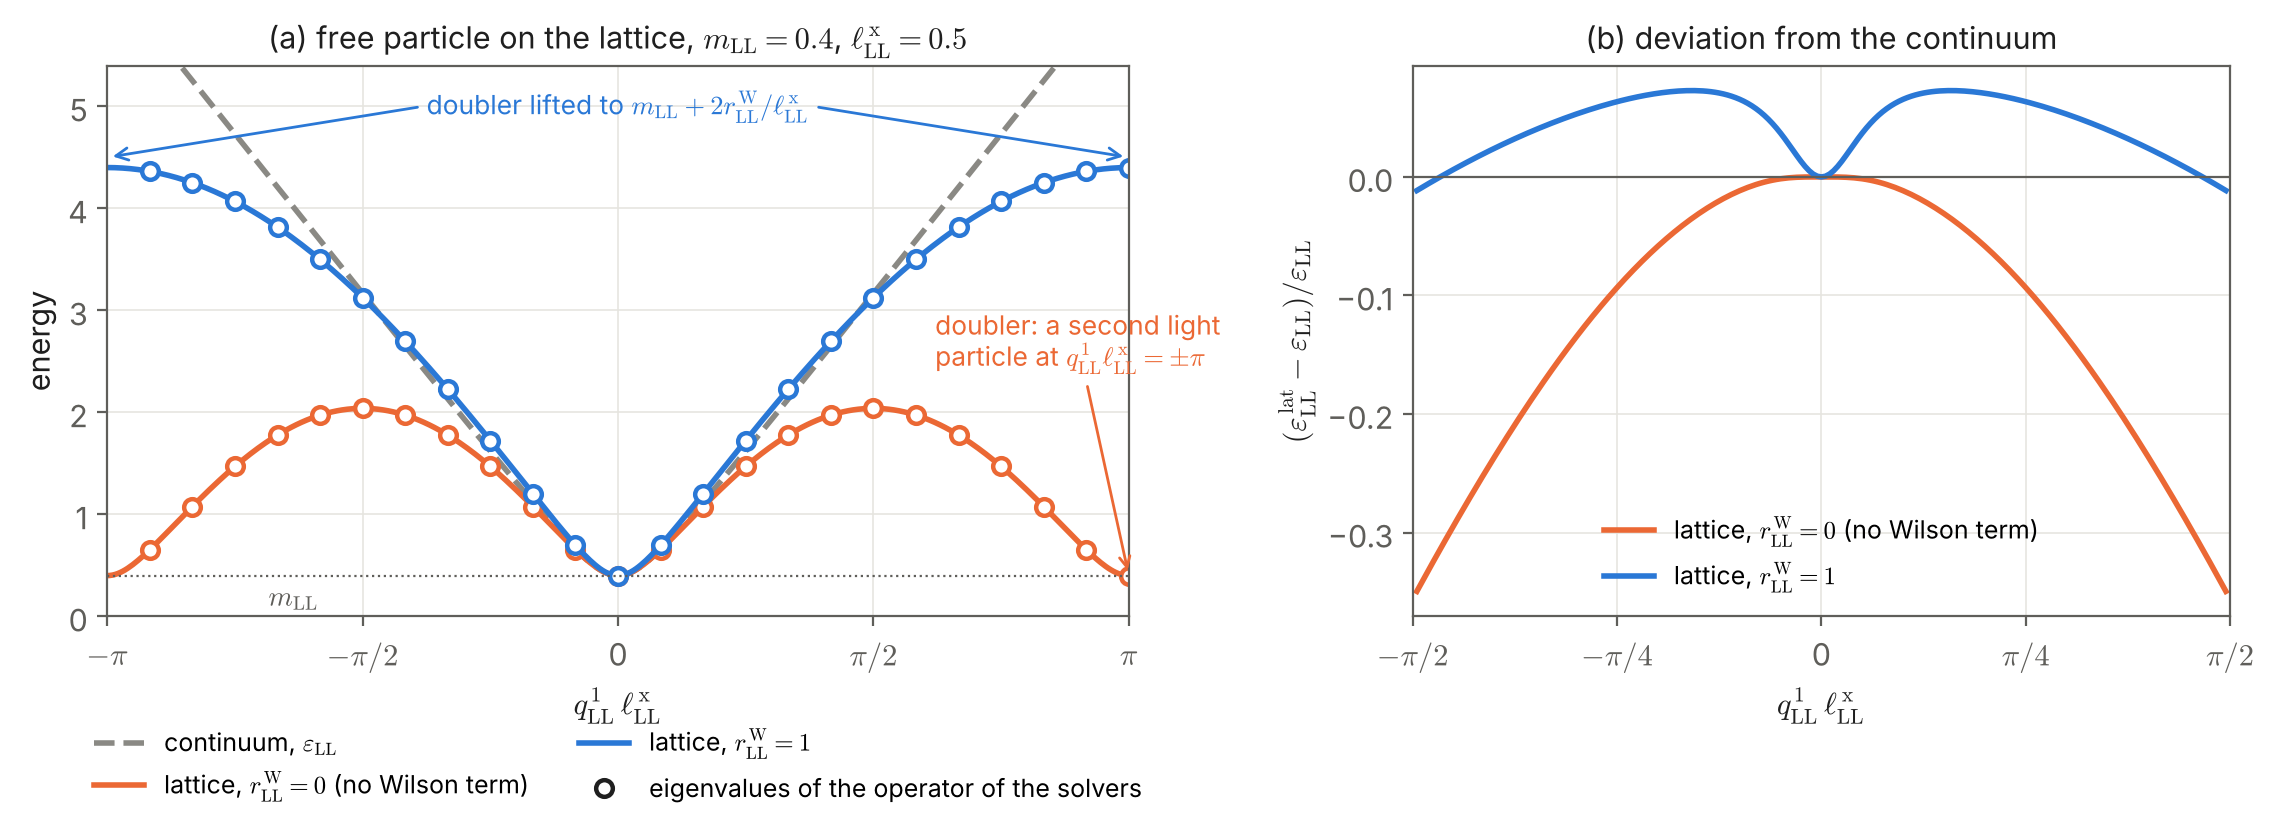
\includegraphics[width=1\textwidth,height=\textheight]{figures/fig_t2_lattice_dispersion.png}

\textbf{Figure 1.} The energy of a free particle on the lattice,
\(\varepsilon^{\rm lat}_{\rm LL}\) of (2.37), along the direction
\(x^1_{\rm LL}\) for \(m_{\rm LL}=0.4\) and
\(\ell^{\rm x}_{\rm LL}=0.5\). (a) Over the whole range of momenta, for
the Wilson coefficients \(r^{\rm W}_{\rm LL}=0\) (orange) and
\(r^{\rm W}_{\rm LL}=1\) (blue), with the continuum energy
\(\varepsilon_{\rm LL}\) (grey, dashed). The circles are the eigenvalues
of the lattice operator of the solvers on the plane waves of a periodic
chain of 24 sites, computed by the routine that the solvers use (check
GS-16); they lie on the curves. (b) The relative deviation from the
continuum,
\((\varepsilon^{\rm lat}_{\rm LL}-\varepsilon_{\rm LL})/\varepsilon_{\rm LL}\),
for the inner half of the momenta. Data:
\texttt{test2/data/t2\_dispersion\_curves.csv},
\texttt{test2/data/t2\_dispersion\_lattice.csv}.

\textbf{Time stepping.} The equations (2.31) on the lattice are a large
system of ordinary differential equations in the time \(x^0_{\rm LL}\),
\(i\partial_0(\psi^{\rm p}_{\rm LL},\psi^{\rm h}_{\rm LL})=\mathcal H^{\rm lat}_{\rm LL}(\psi^{\rm p}_{\rm LL},\psi^{\rm h}_{\rm LL})\).
They are integrated with the classical Runge-Kutta method of fourth
order (RK4) and the time step \(\ell^{\rm t}_{\rm LL}\). For an
eigencomponent with the energy \(E^{\rm qp}_{{\rm LL},n}\) (an
eigenvalue of \(\mathcal H^{\rm lat}_{\rm LL}\)), one step multiplies by
\(1-iE^{\rm qp}_{{\rm LL},n}\ell^{\rm t}_{\rm LL}-\tfrac12(E^{\rm qp}_{{\rm LL},n}\ell^{\rm t}_{\rm LL})^2+\tfrac{i}{6}(E^{\rm qp}_{{\rm LL},n}\ell^{\rm t}_{\rm LL})^3+\tfrac1{24}(E^{\rm qp}_{{\rm LL},n}\ell^{\rm t}_{\rm LL})^4\)
instead of \(\exp(-iE^{\rm qp}_{{\rm LL},n}\ell^{\rm t}_{\rm LL})\). Its
modulus does not exceed 1 for
\(\lvert E^{\rm qp}_{{\rm LL},n}\rvert\ell^{\rm t}_{\rm LL}\le2\sqrt2\)
(stability) and is smaller than 1 by about
\((E^{\rm qp}_{{\rm LL},n}\ell^{\rm t}_{\rm LL})^6/144\) per step
(Figure 2; check GS-13); the phase error per step is about
\((E^{\rm qp}_{{\rm LL},n}\ell^{\rm t}_{\rm LL})^5/120\). The energies
of the lattice operator are bounded by

\[B^{\rm H}_{\rm LL}=\sum_{j\ \text{active}}\frac{1+2r^{\rm W}_{\rm LL}}{\ell^{\rm x}_{\rm LL}}+m_{\rm LL}+\lvert\mu_{\rm LL}\rvert+\max_{\vec s_{\rm LL}}\lVert\mathsf A_{{\rm LL},0}\rVert+\max_{\vec s_{\rm LL}}\sum_\iota\lvert d^\iota_{\rm LL}\rvert\tag{2.38}\]

(the sum over the directions with more than one site;
\(\lVert\cdot\rVert\) the Frobenius norm of the \(2\times2\) isospin
block), so \(\ell^{\rm t}_{\rm LL}\le2.5/B^{\rm H}_{\rm LL}\) is always
stable; the solvers use this bound, and a smaller step where accuracy
for the high energies matters. The links and \(\mathsf A_{{\rm LL},0}\)
of time-dependent gauge fields are evaluated at the times of the four
stages of each step.

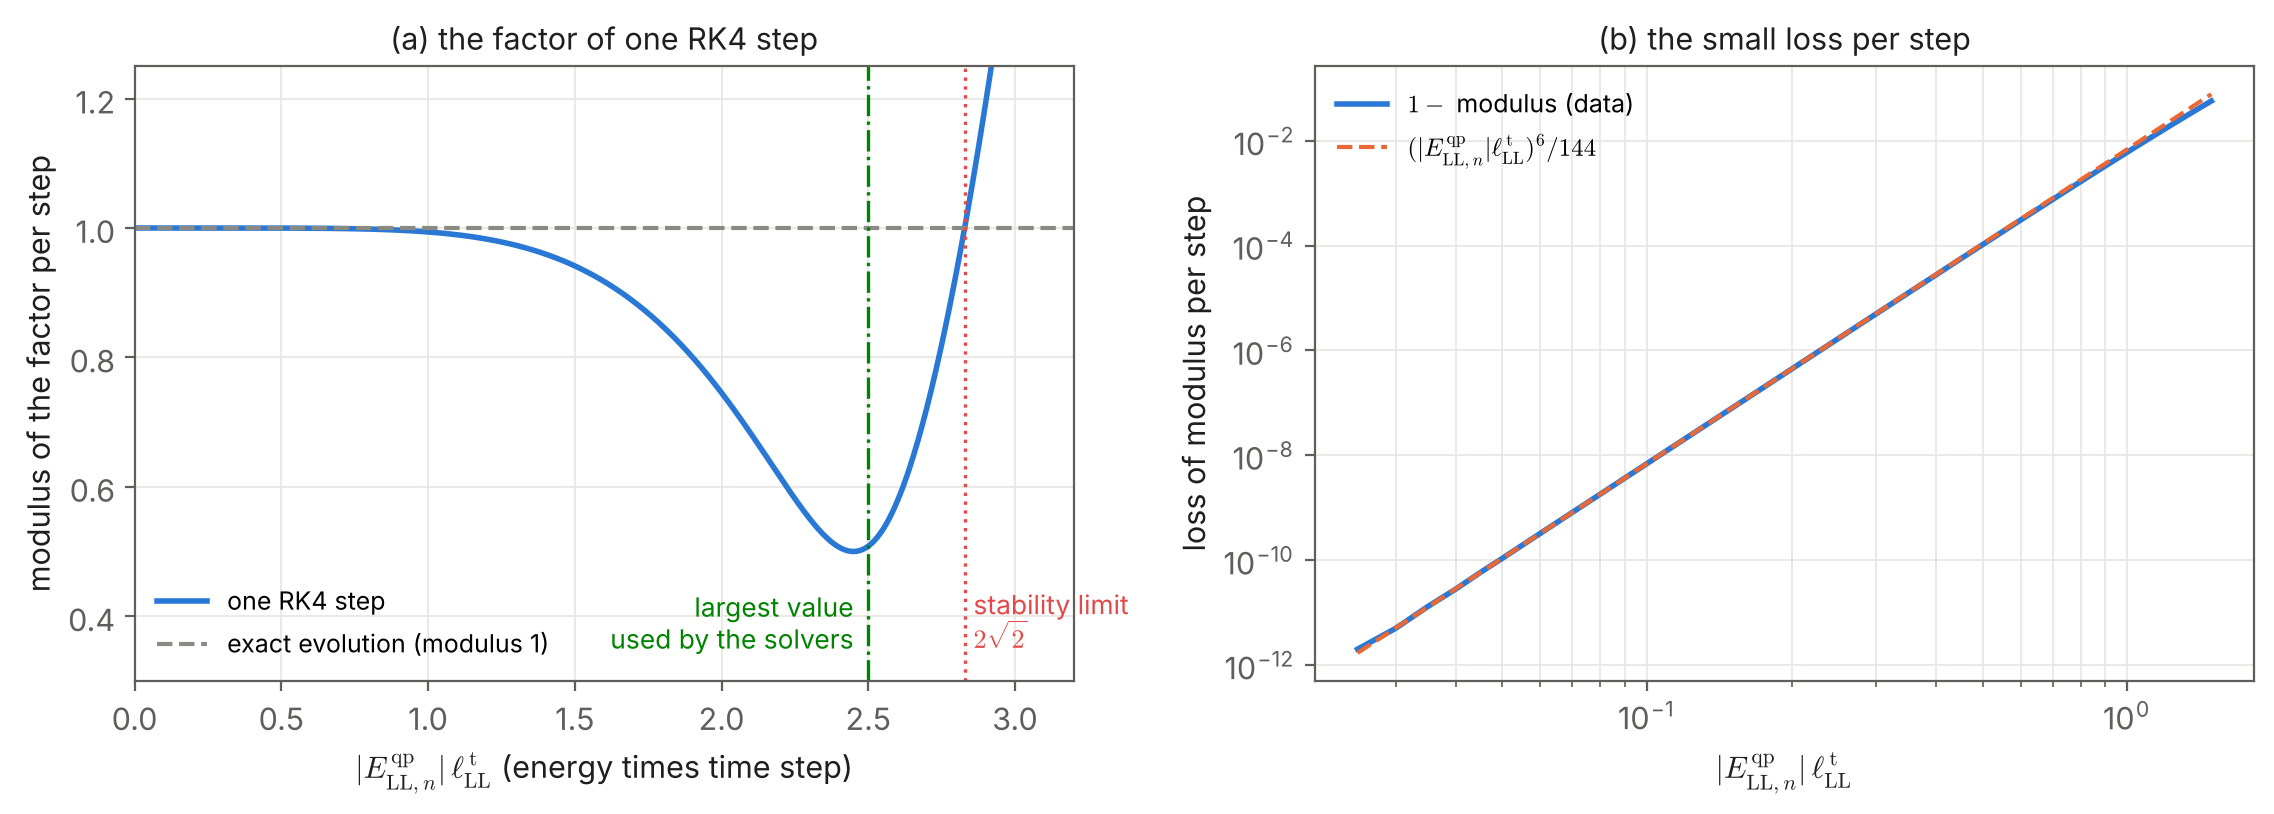
\includegraphics[width=1\textwidth,height=\textheight]{figures/fig_t2_rk4_stability.png}

\textbf{Figure 2.} (a) The modulus of the factor of one RK4 step for an
eigencomponent with the energy \(E^{\rm qp}_{{\rm LL},n}\), as a
function of
\(\lvert E^{\rm qp}_{{\rm LL},n}\rvert\ell^{\rm t}_{\rm LL}\), with the
exact value 1 (grey, dashed), the stability limit \(2\sqrt2\) (red) and
the largest value \(2.5\) that the solvers allow (green). (b) The loss
of modulus per step on logarithmic scales, with the asymptote
\((\lvert E^{\rm qp}_{{\rm LL},n}\rvert\ell^{\rm t}_{\rm LL})^6/144\)
(orange, dashed). Data: \texttt{test2/data/t2\_rk4\_stability.csv}.

\textbf{The stationary ground state.} For the self-consistent use the
initial modes are the eigenvectors of \(\mathcal H^{\rm lat}_{\rm LL}\)
with positive energy, normalized to
\(\sum_{\vec s_{\rm LL}}(\ell^{\rm x}_{\rm LL})^{n^{\rm act}_{\rm LL}}(\lvert\psi^{\rm p}_{\rm LL}\rvert^2+\lvert\psi^{\rm h}_{\rm LL}\rvert^2)=1\),
where \(n^{\rm act}_{\rm LL}\) is the number of directions with more
than one site (3 for a three-dimensional lattice; in problems of fewer
dimensions the densities are per unit length or area of the absent
directions, Section 4.3). They are computed by a Hermitian eigensolver
(in the Rust programs the one of the library \texttt{t2core}:
Householder reduction to a real tridiagonal matrix and the implicit QL
algorithm, check GS-11; in the Python program the routine \texttt{eigh}
of NumPy), and (2.32) is iterated until \(d^\iota_{\rm LL}\) no longer
changes (with the Anderson acceleration of Section 4.3). The
self-consistent evolution of all modes uses the implicit midpoint rule
instead of RK4, because it keeps the modes orthonormal and the fermion
number constant exactly (Section 4.3). This is practical for small
lattices (the matrix has
\(16\,n^{\rm x}_{\rm LL}n^{\rm y}_{\rm LL}n^{\rm z}_{\rm LL}\) rows),
which is the scale of the solvers of items {[}3{]} and {[}5{]}.

\textbf{What the user must specify} (the solvers of items {[}3{]} and
{[}5{]} ask for exactly these): the lattice (\(n^{\rm x}_{\rm LL}\),
\(n^{\rm y}_{\rm LL}\), \(n^{\rm z}_{\rm LL}\),
\(\ell^{\rm x}_{\rm LL}\), \(r^{\rm W}_{\rm LL}\)); the boundary
condition of each direction; the parameters \(m_{\rm LL}\),
\(\mu_{\rm LL}\), \(G_{\rm LL}\), \(g^{\rm v}_{\rm LL}\),
\(g^{\rm F}_{\rm LL}\); the gauge potentials as functions of position
(constant, given on every site, or the Landau gauge of a constant
magnetic field) and of time (a uniform pulse); the pair field
(prescribed or self-consistent); the initial modes (a wave packet, a
plane wave, an eigenmode, or values read from a file); the time step and
the duration; and what is written out.

\textbf{Diagnostics.} The norm of every mode (conserved by (2.31); RK4
loses about \((E^{\rm qp}_{{\rm LL},n}\ell^{\rm t}_{\rm LL})^6/144\) per
step), the orthogonality of the modes, the fermion-number density, the
pair field \(\lvert\vec d_{\rm LL}\rvert\), and, for time-independent
fields, the energy (the sum over the modes of the expectation value of
\(\mathcal H^{\rm lat}_{\rm LL}\)).

\hypertarget{discussion}{%
\subsection{2.12 Discussion}\label{discussion}}

\begin{itemize}
\tightlist
\item
  \textbf{What is specific to the super-loop.} Every ingredient comes
  from the super-loop: the manifold is its Hermitian bi-quaternions; the
  Dirac matrices are its frame multiplications (2.5), (2.13); the
  Lorentz gauge group is its group of unit bi-quaternions acting as
  Lord's change of representation (2.9); the field is made of its spinor
  charges (2.11), on which the gauge group acts by its automorphisms
  (2.14); the covariant derivative is built from its derivations
  \(D_{\rm LL}\) and \(D^{\rm v}_{\rm LL}\) (2.18); the isospin
  generators are
  \(T^\iota_{\rm LL}=i\,D^{\rm v}_{\rm LL}(\mathbf e_\iota/2)\); and the
  self-interaction is its spin-zero pair channel
  \(\mathsf K^\iota_{\rm LL}\). The non-associativity of the
  bi-octonions does not enter the equations of the \(3+1\) manifold: all
  products in (2.11) to (2.18) involve one spinor charge and
  bi-quaternions, for which the Cayley-Dickson rule is associative.
\item
  \textbf{The covariant derivative is in every field equation.} The
  spinor equation (2.25), its Hamiltonian form (2.26), the super-loop
  form (2.28), the mean-field equations (2.31) and their lattice form
  (2.35), (2.36) all contain the derivatives only through
  \(\nabla^{\rm LL}_p\) (or its lattice form, the links); the
  gauge-field equations (2.29) contain the covariant divergence.
\item
  \textbf{The Lorentz gauge field is pure gauge on this flat manifold}
  (Section 2.7). This is the content of Lord's observation in the flat
  case: the gauge freedom of the frame is real, but on Minkowski space
  it carries no field strength. A curved manifold would give
  \(\Gamma^{\rm LL}_p\) a curvature, and Lord's argument then leads to
  general relativity; that is beyond the \(3+1\) manifold of the
  super-loop.
\item
  \textbf{Limits of the formulation.} The mean-field approximation
  neglects the fluctuations of the pair field (they are the subject of
  items {[}8{]} to {[}11{]}); the internal gauge fields are external in
  the solvers; the lattice computation of the self-consistent ground
  state is limited to small lattices. Each of these is a choice of the
  numerical method, not of the field equations (2.25) and (2.29), which
  are exact.
\end{itemize}

\hypertarget{item-2-analysis-of-the-field-equations-and-analytic-solutions}{%
\section{3. Item {[}2{]}: analysis of the field equations, and analytic
solutions}\label{item-2-analysis-of-the-field-equations-and-analytic-solutions}}

\hypertarget{the-answer-in-brief-1}{%
\subsection{3.0 The answer in brief}\label{the-answer-in-brief-1}}

Item {[}2{]} asks for an analysis of the field equations of Section 2
and for analytic solutions of at least three simple cases. Section 3.1
analyzes the equations: which quantities they conserve, why the fermion
number is conserved only when the pair field is self-consistent, what
the gauge covariance implies for constant potentials, how plane waves
turn the equations into matrix equations, and what the square of the
covariant Dirac Hamiltonian is (it gives the Pauli equation of slow
spinor charges, with the gyromagnetic factor 2 for both kinds of
charge). Sections 3.2 to 3.5 then solve four cases exactly:

\begin{longtable}[]{@{}
  >{\raggedright\arraybackslash}p{(\columnwidth - 6\tabcolsep) * \real{0.0659}}
  >{\raggedright\arraybackslash}p{(\columnwidth - 6\tabcolsep) * \real{0.3297}}
  >{\raggedright\arraybackslash}p{(\columnwidth - 6\tabcolsep) * \real{0.5055}}
  >{\raggedright\arraybackslash}p{(\columnwidth - 6\tabcolsep) * \real{0.0989}}@{}}
\toprule\noalign{}
\begin{minipage}[b]{\linewidth}\raggedright
case
\end{minipage} & \begin{minipage}[b]{\linewidth}\raggedright
fields
\end{minipage} & \begin{minipage}[b]{\linewidth}\raggedright
analytic solution
\end{minipage} & \begin{minipage}[b]{\linewidth}\raggedright
checks
\end{minipage} \\
\midrule\noalign{}
\endhead
\bottomrule\noalign{}
\endlastfoot
A & constant gauge potentials, no pair field & plane waves whose
momentum is shifted by the space components of the potential and whose
energy is shifted by its time component (3.7); a constant isospin
potential turns the isospin (3.8) & AS-1, AS-2 \\
B & uniform pair field \(d^\iota_{\rm LL}=(0,0,\Delta_{\rm LL})\) (the
polar superfluid) & the Bogoliubov modes and their energies
\(\pm E^\pm_{\rm LL}\) (3.13), (3.14); the particle-hole oscillation of
an injected particle (3.16); the gap equation (2.33) in closed form
(3.17) and its weak-coupling limit (3.20); the uniform state as an exact
self-consistent solution on the lattice (3.21) & AS-3 to AS-6 \\
C & a domain wall (kink) of the pair field & bound states at exactly
\(\pm m_{\rm LL}\) (3.24); the square of the operator (3.25) and the
complete spectrum of the bound states (3.28); the bound states on the
lattice and the first-order effect of the Wilson term (3.29) & AS-7 to
AS-9 \\
D & constant magnetic fields & Landau levels (3.32) & AS-10 \\
\end{longtable}

Every analytic solution is checked twice by the program
\texttt{t2\_analytic} (folder \texttt{test2/rust}; checks AS-1 to AS-10,
report in Appendix A): against the continuum equations (2.31), and
against the lattice operator (2.36), which is the operator that the
solvers of items {[}3{]} and {[}5{]} integrate. The time-dependent
solutions are compared with the RK4 integration of the lattice
equations. These solutions are therefore also test problems with known
answers for the solvers. Figures 3 to 6 show them. All four cases are
computed in the canonical gauge \(\Gamma^{\rm LL}_p=0\) of Section 2.7;
the gauge transformation (2.10) carries each solution into any other
gauge.

\hypertarget{analysis-of-the-field-equations}{%
\subsection{3.1 Analysis of the field
equations}\label{analysis-of-the-field-equations}}

\textbf{The equations.} In the canonical gauge the mean-field equations
(2.31) are

\[i\partial_0\psi^{\rm p}_{\rm LL}=\big(h^\nabla_{\rm LL}-\mathsf A_{{\rm LL},0}-\mu_{\rm LL}\big)\psi^{\rm p}_{\rm LL}+\mathsf P_{\rm LL}\psi^{\rm h}_{\rm LL},\qquad i\partial_0\psi^{\rm h}_{\rm LL}=\mathsf P^\dagger_{\rm LL}\psi^{\rm p}_{\rm LL}-\big(h^\nabla_{\rm LL}-\mathsf A_{{\rm LL},0}-\mu_{\rm LL}\big)^*\psi^{\rm h}_{\rm LL},\tag{3.1}\]

with the covariant Dirac Hamiltonian
\(h^\nabla_{\rm LL}=-i\sum_j\alpha^j_{\rm LL}\nabla^{\rm LL}_j+\beta_{\rm LL}m_{\rm LL}\),
the covariant derivative
\(\nabla^{\rm LL}_j=\partial_j-i\mathsf A_{{\rm LL},j}\), the
\(2\times2\) isospin matrices of the potentials
\(\mathsf A_{{\rm LL},p}=g^{\rm v}_{\rm LL}\sum_\iota A^\iota_{{\rm LL},p}T^\iota_{\rm LL}+g^{\rm F}_{\rm LL}A^{\rm F}_{{\rm LL},p}\),
and the pairing block
\(\mathsf P_{\rm LL}=\sum_\iota d^\iota_{\rm LL}(\mathsf K^\iota_{\rm LL})^\dagger\).
The matrices
\(\alpha^j_{\rm LL}=\mathrm{diag}(-\sigma^{\rm LL}_j,\sigma^{\rm LL}_j)\)
and \(\beta_{\rm LL}=\gamma^0_{\rm LL}\) act on the Dirac index,
\(\mathsf A_{{\rm LL},p}\) on the isospin index. Two kinds of problems
are distinguished. If the gauge fields and the pair field are given
(prescribed), (3.1) is linear in each mode: sums of solutions are
solutions, and each mode can be studied by itself. If
\(d^\iota_{\rm LL}\) is computed from the modes by (2.32), the system is
nonlinear. Cases A, C and D below have prescribed fields; the uniform
pair field of case B is also an exact self-consistent solution (Section
3.3).

\textbf{Each mode keeps its norm.} Multiply the first equation of (3.1)
from the left by \((\psi^{\rm p}_{\rm LL})^\dagger\), the second by
\((\psi^{\rm h}_{\rm LL})^\dagger\), and add to each the complex
conjugate of the equation multiplied in the same way. The terms with
\(\beta_{\rm LL}m_{\rm LL}\), \(\mathsf A_{{\rm LL},0}\) and
\(\mu_{\rm LL}\) drop out, because these are Hermitian matrices; the
potentials in \(\nabla^{\rm LL}_j\) drop out for the same reason (they
act on the isospin index and commute with \(\alpha^j_{\rm LL}\)); the
remaining derivative terms combine into divergences. What remains is

\[\begin{aligned}\partial_0\lvert\psi^{\rm p}_{\rm LL}\rvert^2+\sum_j\partial_j\big((\psi^{\rm p}_{\rm LL})^\dagger\alpha^j_{\rm LL}\psi^{\rm p}_{\rm LL}\big)&=2\,\mathrm{Im}\big((\psi^{\rm p}_{\rm LL})^\dagger\mathsf P_{\rm LL}\psi^{\rm h}_{\rm LL}\big),\\\partial_0\lvert\psi^{\rm h}_{\rm LL}\rvert^2+\sum_j\partial_j\big((\psi^{\rm h}_{\rm LL})^\dagger(\alpha^j_{\rm LL})^*\psi^{\rm h}_{\rm LL}\big)&=-2\,\mathrm{Im}\big((\psi^{\rm p}_{\rm LL})^\dagger\mathsf P_{\rm LL}\psi^{\rm h}_{\rm LL}\big).\end{aligned}\tag{3.2}\]

Added, the right sides cancel: the density
\(\lvert\psi^{\rm p}_{\rm LL}\rvert^2+\lvert\psi^{\rm h}_{\rm LL}\rvert^2\)
of each mode obeys a continuity equation, and the norm
\(\int d^3\vec x_{\rm LL}(\lvert\psi^{\rm p}_{\rm LL}\rvert^2+\lvert\psi^{\rm h}_{\rm LL}\rvert^2)\)
of each mode is constant (for modes that vanish at infinity or are
periodic). This is the statement that \(\mathcal H^{\rm DB}_{\rm LL}\)
is Hermitian, written locally. Separately, the particle part and the
hole part of a mode are not conserved: the pair field converts the one
into the other (case B, (3.16)).

\textbf{The fermion number is conserved when, and only when, the pair
field is self-consistent.} The density of the fermion number in the
state is \(\sum_n\lvert\psi^{\rm h}_{{\rm LL},n}\rvert^2\) and its
current
\(\sum_n(\psi^{\rm h}_{{\rm LL},n})^\dagger(\alpha^j_{\rm LL})^*\psi^{\rm h}_{{\rm LL},n}\)
(Section 2.10; the sums run over the modes of the state). By the second
equation (3.2), summed over the modes, the source of the fermion number
is
\(-2\,\mathrm{Im}\sum_n(\psi^{\rm p}_{{\rm LL},n})^\dagger\mathsf P_{\rm LL}\psi^{\rm h}_{{\rm LL},n}\).
The pair matrices are antisymmetric (check GS-4), so
\((\mathsf K^\iota_{\rm LL})^\dagger=-(\mathsf K^\iota_{\rm LL})^*\) and
\((\psi^{\rm p}_{{\rm LL},n})^\dagger(\mathsf K^\iota_{\rm LL})^\dagger\psi^{\rm h}_{{\rm LL},n}=-\big((\psi^{\rm p}_{{\rm LL},n})^T\mathsf K^\iota_{\rm LL}(\psi^{\rm h}_{{\rm LL},n})^*\big)^*\).
If the pair field obeys (2.32), the sum over the modes of the bracket is
\(-2d^\iota_{\rm LL}/G_{\rm LL}\), and

\[\sum_n(\psi^{\rm p}_{{\rm LL},n})^\dagger\mathsf P_{\rm LL}\psi^{\rm h}_{{\rm LL},n}=\sum_\iota d^\iota_{\rm LL}\,\frac{2(d^\iota_{\rm LL})^*}{G_{\rm LL}}=\frac2{G_{\rm LL}}\sum_\iota\lvert d^\iota_{\rm LL}\rvert^2,\tag{3.3}\]

which is real: the source vanishes at every point. With a
self-consistent pair field the fermion number is exactly conserved, as
the invariance under the phase group \(U(1)^{\rm F}_{\rm LL}\) requires;
with a prescribed pair field it is not. The total fermion number is
therefore a check of the self-consistent solvers.

\textbf{Constant potentials are pure gauge.} The gauge transformation
(2.10) acts on the modes by
\(\psi^{\rm p}_{\rm LL}\mapsto\exp(i\theta^{\rm F}_{\rm LL})\mathsf U_{\rm LL}\psi^{\rm p}_{\rm LL}\)
and on the potentials by
\(A^{\rm F}_{{\rm LL},p}\mapsto A^{\rm F}_{{\rm LL},p}+\partial_p\theta^{\rm F}_{\rm LL}/g^{\rm F}_{\rm LL}\)
and
\(\mathsf a_{{\rm LL},p}\mapsto\mathsf U_{\rm LL}\mathsf a_{{\rm LL},p}\mathsf U^{-1}_{\rm LL}-(i/g^{\rm v}_{\rm LL})(\partial_p\mathsf U_{\rm LL})\mathsf U^{-1}_{\rm LL}\)
(check GS-5). Applied to zero potentials with
\(\theta^{\rm F}_{\rm LL}=g^{\rm F}_{\rm LL}\sum_pA^{\rm F}_{{\rm LL},p}x^p_{\rm LL}\)
and
\(\mathsf U_{\rm LL}=\exp\big(\tfrac i2g^{\rm v}_{\rm LL}\sum_pA^3_{{\rm LL},p}x^p_{\rm LL}\,\tau^{\rm LL}_3\big)\)
for constant numbers \(A^{\rm F}_{{\rm LL},p}\), \(A^3_{{\rm LL},p}\),
it gives exactly these constant potentials:
\(\partial_p\theta^{\rm F}_{\rm LL}/g^{\rm F}_{\rm LL}=A^{\rm F}_{{\rm LL},p}\)
and
\(-(i/g^{\rm v}_{\rm LL})(\partial_p\mathsf U_{\rm LL})\mathsf U^{-1}_{\rm LL}=\tfrac12A^3_{{\rm LL},p}\tau^{\rm LL}_3\).
Constant potentials of one isospin direction have zero field strength
(the commutator term of \(\mathsf F^\iota_{{\rm LL},pp'}\) needs two
different isospin directions). In infinite space, therefore, the
solutions with such potentials are the free solutions multiplied by
\(\exp(i\theta^{\rm F}_{\rm LL})\mathsf U_{\rm LL}\), and nothing
observable changes. On a periodic lattice of \(n^{\rm x}_{\rm LL}\)
sites, of the circumference \(n^{\rm x}_{\rm LL}\ell^{\rm x}_{\rm LL}\),
the gauge function must be periodic; this fails unless
\(\exp(i\mathsf A_{{\rm LL},1}n^{\rm x}_{\rm LL}\ell^{\rm x}_{\rm LL})\)
is the unit matrix. This matrix is the gauge-invariant product of the
link matrices around the ring (the holonomy, or Wilson loop): if it is
not the unit matrix, the ring encloses a magnetic flux that no gauge
transformation removes, and the energies of the allowed momenta are
shifted (the Aharonov-Bohm effect, case A).

\textbf{Plane waves.} If all fields are independent of the position
(constant potentials, a uniform pair field), (3.1) has the solutions
\(\exp(i\sum_jq^j_{\rm LL}x^j_{\rm LL}-iE^{\rm qp}_{{\rm LL},n}x^0_{\rm LL})\)
times a constant 16-component vector, which must be an eigenvector of
the \(16\times16\) matrix
\(\mathcal H^{\rm DB}_{\rm LL}(\vec q_{\rm LL})\) with the eigenvalue
\(E^{\rm qp}_{{\rm LL},n}\) (check GS-8). The field equations become
matrix algebra. On the lattice the same holds with
\(\sin(q^j_{\rm LL}\ell^{\rm x}_{\rm LL})/\ell^{\rm x}_{\rm LL}\) in
place of \(q^j_{\rm LL}\) and the Wilson term added to the mass, (2.37);
on a periodic lattice the momenta are the integer multiples of
\(2\pi/(n^{\rm x}_{\rm LL}\ell^{\rm x}_{\rm LL})\).

\textbf{The square of the covariant Dirac Hamiltonian.} The Dirac
matrices satisfy
\(\alpha^j_{\rm LL}\alpha^{j'}_{\rm LL}+\alpha^{j'}_{\rm LL}\alpha^j_{\rm LL}=2\)
for \(j=j'\) and \(0\) for \(j\ne j'\),
\(\alpha^j_{\rm LL}\beta_{\rm LL}+\beta_{\rm LL}\alpha^j_{\rm LL}=0\),
\(\beta_{\rm LL}^2=\mathsf 1_4\), and, for the three cyclic triples
\((j,j',j'')=(1,2,3),(2,3,1),(3,1,2)\),
\(\alpha^j_{\rm LL}\alpha^{j'}_{\rm LL}=-\gamma^j_{\rm LL}\gamma^{j'}_{\rm LL}=-2\,\mathsf s_{\rm LL}(J^{j''}_{\rm LL})\)
(check GS-2:
\(\mathsf s_{\rm LL}(J^{j''}_{\rm LL})=\gamma^j_{\rm LL}\gamma^{j'}_{\rm LL}/2=\mathrm{diag}(-i\sigma^{\rm LL}_{j''},-i\sigma^{\rm LL}_{j''})/2\)).
In the square of \(h^\nabla_{\rm LL}\) the terms with
\(\alpha^j_{\rm LL}\beta_{\rm LL}\) cancel, the terms with \(j=j'\) give
\(\sum_j(-i\nabla^{\rm LL}_j)^2\), and the terms with \(j\ne j'\)
combine into commutators,
\(-\sum_{\rm cyclic}\alpha^j_{\rm LL}\alpha^{j'}_{\rm LL}[\nabla^{\rm LL}_j,\nabla^{\rm LL}_{j'}]\).
With the commutator of two covariant derivatives,
\([\nabla^{\rm LL}_j,\nabla^{\rm LL}_{j'}]=-i\big(g^{\rm v}_{\rm LL}\sum_\iota\mathsf F^\iota_{{\rm LL},jj'}T^\iota_{\rm LL}+g^{\rm F}_{\rm LL}\mathsf F^{\rm F}_{{\rm LL},jj'}\big)\)
(check GS-6, canonical gauge), this is

\[(h^\nabla_{\rm LL})^2=m_{\rm LL}^2+\sum_j(-i\nabla^{\rm LL}_j)^2-2\sum_{(j,j',j'')\ \text{cyclic}}i\,\mathsf s_{\rm LL}(J^{j''}_{\rm LL})\Big(g^{\rm v}_{\rm LL}\sum_\iota\mathsf F^\iota_{{\rm LL},jj'}T^\iota_{\rm LL}+g^{\rm F}_{\rm LL}\mathsf F^{\rm F}_{{\rm LL},jj'}\Big),\tag{3.4}\]

where
\(i\,\mathsf s_{\rm LL}(J^{j''}_{\rm LL})=\tfrac12\mathrm{diag}(\sigma^{\rm LL}_{j''},\sigma^{\rm LL}_{j''})\)
is the spin of the spinor charge along \(x^{j''}_{\rm LL}\); the field
strengths with \((j,j')=(1,2)\), \((2,3)\), \((3,1)\) are the magnetic
fields along \(x^3_{\rm LL}\), \(x^1_{\rm LL}\), \(x^2_{\rm LL}\).
Equation (3.4) is exact. On the states of positive energy,
\(h^\nabla_{\rm LL}\) is the positive square root of (3.4); for slow
spinor charges in static magnetic fields (the last two terms of (3.4)
small compared with \(m_{\rm LL}^2\)) the expansion of the square root
gives

\[h^\nabla_{\rm LL}\approx m_{\rm LL}+\frac1{2m_{\rm LL}}\sum_j(-i\nabla^{\rm LL}_j)^2-\frac1{m_{\rm LL}}\sum_{(j,j',j'')\ \text{cyclic}}i\,\mathsf s_{\rm LL}(J^{j''}_{\rm LL})\Big(g^{\rm v}_{\rm LL}\sum_\iota\mathsf F^\iota_{{\rm LL},jj'}T^\iota_{\rm LL}+g^{\rm F}_{\rm LL}\mathsf F^{\rm F}_{{\rm LL},jj'}\Big):\tag{3.5}\]

the rest energy, the kinetic energy of the covariant momentum
\(-i\nabla^{\rm LL}_j\), and the energy of a magnetic moment, which is
the charge divided by \(2m_{\rm LL}\), times 2, times the spin. The
factor 2 (the gyromagnetic factor of Dirac particles) holds for the
phase charge \(g^{\rm F}_{\rm LL}\) and for the isospin charges
\(g^{\rm v}_{\rm LL}T^\iota_{\rm LL}\) alike. With the potential energy
\(-\mathsf A_{{\rm LL},0}\) added, (3.5) is the Pauli equation of the
spinor charges. Case D uses (3.4) without approximation.

\textbf{Particle-hole symmetry.} Every spectrum below is symmetric about
zero: with each mode of energy \(E^{\rm qp}_{{\rm LL},n}\) the exchanged
mode of Section 2.10 has the energy \(-E^{\rm qp}_{{\rm LL},n}\) (check
GS-8).

\hypertarget{case-a-free-spinor-charges-in-constant-gauge-potentials}{%
\subsection{3.2 Case A: free spinor charges in constant gauge
potentials}\label{case-a-free-spinor-charges-in-constant-gauge-potentials}}

\textbf{The fields.} No pair field (\(d^\iota_{\rm LL}=0\)). Constant
potentials of the phase group and of the third isospin direction,
\(A^{\rm F}_{{\rm LL},p}\) and \(A^3_{{\rm LL},p}\), with
\(A^1_{{\rm LL},p}=A^2_{{\rm LL},p}=0\). Then \(T^3_{\rm LL}\) is
diagonal and the isospin matrices of the potentials are

\[\mathsf A_{{\rm LL},p}=\begin{pmatrix}\mathsf A^\uparrow_{{\rm LL},p}&0\\0&\mathsf A^\downarrow_{{\rm LL},p}\end{pmatrix},\qquad\mathsf A^\uparrow_{{\rm LL},p}=g^{\rm F}_{\rm LL}A^{\rm F}_{{\rm LL},p}+\tfrac12g^{\rm v}_{\rm LL}A^3_{{\rm LL},p},\qquad\mathsf A^\downarrow_{{\rm LL},p}=g^{\rm F}_{\rm LL}A^{\rm F}_{{\rm LL},p}-\tfrac12g^{\rm v}_{\rm LL}A^3_{{\rm LL},p}.\tag{3.6}\]

\(\mathsf A^\uparrow_{{\rm LL},p}\) acts on the isospin-up components
(the charge \(Q_{\rm LL}=T^3_{\rm LL}=+\tfrac12\)),
\(\mathsf A^\downarrow_{{\rm LL},p}\) on the isospin-down components
(\(Q_{\rm LL}=-\tfrac12\)). The field strengths vanish.

\textbf{The solution.} Try a particle of isospin up,
\(\psi^{\rm p}_{\rm LL}=\exp\big(i\sum_jq^j_{\rm LL}x^j_{\rm LL}-iE^{\rm qp}_{{\rm LL},n}x^0_{\rm LL}\big)\chi^{\rm pw}_{\rm LL}\),
where \(\chi^{\rm pw}_{\rm LL}\) is a constant 4-component Dirac spinor
times the isospin vector \((1,0)^T\), and \(\psi^{\rm h}_{\rm LL}=0\).
The covariant derivative gives
\(\nabla^{\rm LL}_j\psi^{\rm p}_{\rm LL}=i(q^j_{\rm LL}-\mathsf A^\uparrow_{{\rm LL},j})\psi^{\rm p}_{\rm LL}\),
and (3.1) becomes the eigenvalue problem
\(E^{\rm qp}_{{\rm LL},n}\chi^{\rm pw}_{\rm LL}=\big(\sum_j\alpha^j_{\rm LL}(q^j_{\rm LL}-\mathsf A^\uparrow_{{\rm LL},j})+\beta_{\rm LL}m_{\rm LL}-\mathsf A^\uparrow_{{\rm LL},0}-\mu_{\rm LL}\big)\chi^{\rm pw}_{\rm LL}\).
By the anticommutation relations of Section 3.1 the matrix
\(\sum_j\alpha^j_{\rm LL}(q^j_{\rm LL}-\mathsf A^\uparrow_{{\rm LL},j})+\beta_{\rm LL}m_{\rm LL}\)
squares to
\(\sum_j(q^j_{\rm LL}-\mathsf A^\uparrow_{{\rm LL},j})^2+m_{\rm LL}^2\)
times the unit matrix, so its eigenvalues are the two square roots, each
twice. The hole (with \(\psi^{\rm p}_{\rm LL}=0\)) is treated in the
same way with the operator
\(-(h^\nabla_{\rm LL}-\mathsf A_{{\rm LL},0}-\mu_{\rm LL})^*\), in which
the charges have the opposite sign. The energies are

\[\begin{aligned}\text{particles: }E^{\rm qp}_{{\rm LL},n}&=\pm\Big(\sum_j(q^j_{\rm LL}-\mathsf A^\uparrow_{{\rm LL},j})^2+m_{\rm LL}^2\Big)^{1/2}-\mathsf A^\uparrow_{{\rm LL},0}-\mu_{\rm LL},\\\text{holes: }E^{\rm qp}_{{\rm LL},n}&=\mp\Big(\sum_j(q^j_{\rm LL}+\mathsf A^\uparrow_{{\rm LL},j})^2+m_{\rm LL}^2\Big)^{1/2}+\mathsf A^\uparrow_{{\rm LL},0}+\mu_{\rm LL},\end{aligned}\tag{3.7}\]

each twice, and the same with \(\mathsf A^\downarrow_{{\rm LL},p}\) for
isospin down. On the lattice the square roots are replaced by
\(\varepsilon^{\rm lat}_{\rm LL}\) of (2.37) at the shifted momenta.
This is exact on the lattice: the link
\(\mathsf U^{\rm link}_{{\rm LL},1}=\exp(-i\ell^{\rm x}_{\rm LL}\mathsf A_{{\rm LL},1})\)
multiplies the plane wave at the next site,
\(\exp(iq^1_{\rm LL}(x^1_{\rm LL}+\ell^{\rm x}_{\rm LL}))\), by
\(\exp(-i\ell^{\rm x}_{\rm LL}\mathsf A^\uparrow_{{\rm LL},1})\), which
shifts the momentum in the covariant difference (2.35) by exactly
\(\mathsf A^\uparrow_{{\rm LL},1}\).

\textbf{What it shows.} The space components of the potential shift the
momentum: the plane wave labelled by the momentum \(q^j_{\rm LL}\) (the
canonical momentum) moves with the kinetic momentum
\(q^j_{\rm LL}-\mathsf A^\uparrow_{{\rm LL},j}\), and the bottom of the
band lies at \(q^1_{\rm LL}=\mathsf A^\uparrow_{{\rm LL},1}\) (minimal
coupling). The time component shifts the energy, exactly as a change of
the chemical potential would:
\(\mathsf A^\uparrow_{{\rm LL},0}+\mu_{\rm LL}\) enters as a whole. In
infinite space both shifts are pure gauge (Section 3.1). On the ring of
check AS-1 (\(n^{\rm x}_{\rm LL}=32\), \(\ell^{\rm x}_{\rm LL}=0.5\),
circumference 16) the holonomy
\(\exp(i\cdot16\,\mathsf A^\uparrow_{{\rm LL},1})\) with
\(\mathsf A^\uparrow_{{\rm LL},1}=0.55\) is not 1, and the energies at
the allowed momenta are truly shifted. Figure 3(a) shows (3.7) for both
isospin components and the eigenvalues of the lattice operator of the
solvers on the plane waves of the ring; they agree to \(10^{-14}\)
(check AS-1).

\textbf{The isospin turns in a constant isospin potential.} Now let only
\(A^1_{{\rm LL},0}\) be non-zero (and constant):
\(\mathsf A_{{\rm LL},0}=\tfrac12g^{\rm v}_{\rm LL}A^1_{{\rm LL},0}\tau^{\rm LL}_1\).
This matrix acts on the isospin index and commutes with
\(h^\nabla_{\rm LL}\), so the evolution operator of the particle row
factorizes,
\(\exp\big(-i(h^\nabla_{\rm LL}-\mathsf A_{{\rm LL},0}-\mu_{\rm LL})x^0_{\rm LL}\big)=\exp\big(-i(h^\nabla_{\rm LL}-\mu_{\rm LL})x^0_{\rm LL}\big)\exp(i\mathsf A_{{\rm LL},0}x^0_{\rm LL})\),
and
\(\exp(i\mathsf A_{{\rm LL},0}x^0_{\rm LL})=\cos(\omega^{\rm pr}_{\rm LL}x^0_{\rm LL}/2)\,\sigma^{\rm LL}_0+i\sin(\omega^{\rm pr}_{\rm LL}x^0_{\rm LL}/2)\,\tau^{\rm LL}_1\)
with \(\omega^{\rm pr}_{\rm LL}=g^{\rm v}_{\rm LL}A^1_{{\rm LL},0}\)
(because \((\tau^{\rm LL}_1)^2=\sigma^{\rm LL}_0\)). A particle that
starts as a plane wave of positive energy \(\varepsilon_{\rm LL}\) with
isospin up,
\(\chi^{\rm pw}_{\rm LL}=(\text{Dirac spinor})\otimes(1,0)^T\),
therefore evolves as

\[\begin{aligned}\psi^{\rm p}_{\rm LL}(x_{\rm LL})&=\exp\Big(i\sum_jq^j_{\rm LL}x^j_{\rm LL}-i(\varepsilon_{\rm LL}-\mu_{\rm LL})x^0_{\rm LL}\Big)\,(\text{Dirac spinor})\otimes\begin{pmatrix}\cos(\omega^{\rm pr}_{\rm LL}x^0_{\rm LL}/2)\\i\sin(\omega^{\rm pr}_{\rm LL}x^0_{\rm LL}/2)\end{pmatrix},\\P^\uparrow_{\rm LL}(x^0_{\rm LL})&=\cos^2(\omega^{\rm pr}_{\rm LL}x^0_{\rm LL}/2).\end{aligned}\tag{3.8}\]

The isospin turns about the direction of the potential (here
\(\tau^{\rm LL}_1\)) with the angular frequency
\(\omega^{\rm pr}_{\rm LL}\), and the probability
\(P^\uparrow_{\rm LL}\) of isospin up oscillates. In the same way, for a
potential of any isospin direction,

\[\omega^{\rm pr}_{\rm LL}=g^{\rm v}_{\rm LL}\Big(\sum_\iota(A^\iota_{{\rm LL},0})^2\Big)^{1/2}.\tag{3.9}\]

\emph{Meaning.} This potential has zero field strength, and the rotation
(3.8) is exactly the gauge transformation
\(\mathsf U_{\rm LL}=\exp(i\mathsf A_{{\rm LL},0}x^0_{\rm LL})\) that
removes it: in the gauge in which \(\mathsf A_{{\rm LL},0}=0\), the
isospin of the same particle stays up. The isospin direction of a single
mode is therefore not gauge invariant; only its direction relative to
other isospin-carrying objects is (for example relative to a pair field
\(d^\iota_{\rm LL}\), which the gauge transformation turns as well). The
potential acts as an isospin chemical potential: the energies of the
isospin states along \(\tau^{\rm LL}_1\) are
\(\varepsilon_{\rm LL}-\mu_{\rm LL}\mp\omega^{\rm pr}_{\rm LL}/2\). For
the solvers this is a sharp test of the isospin structure of the
potential term: the RK4 integration of the lattice equations reproduces
(3.8) with the relative deviation \(9\times10^{-10}\), the size of the
RK4 phase error (Figure 3(b), check AS-2).

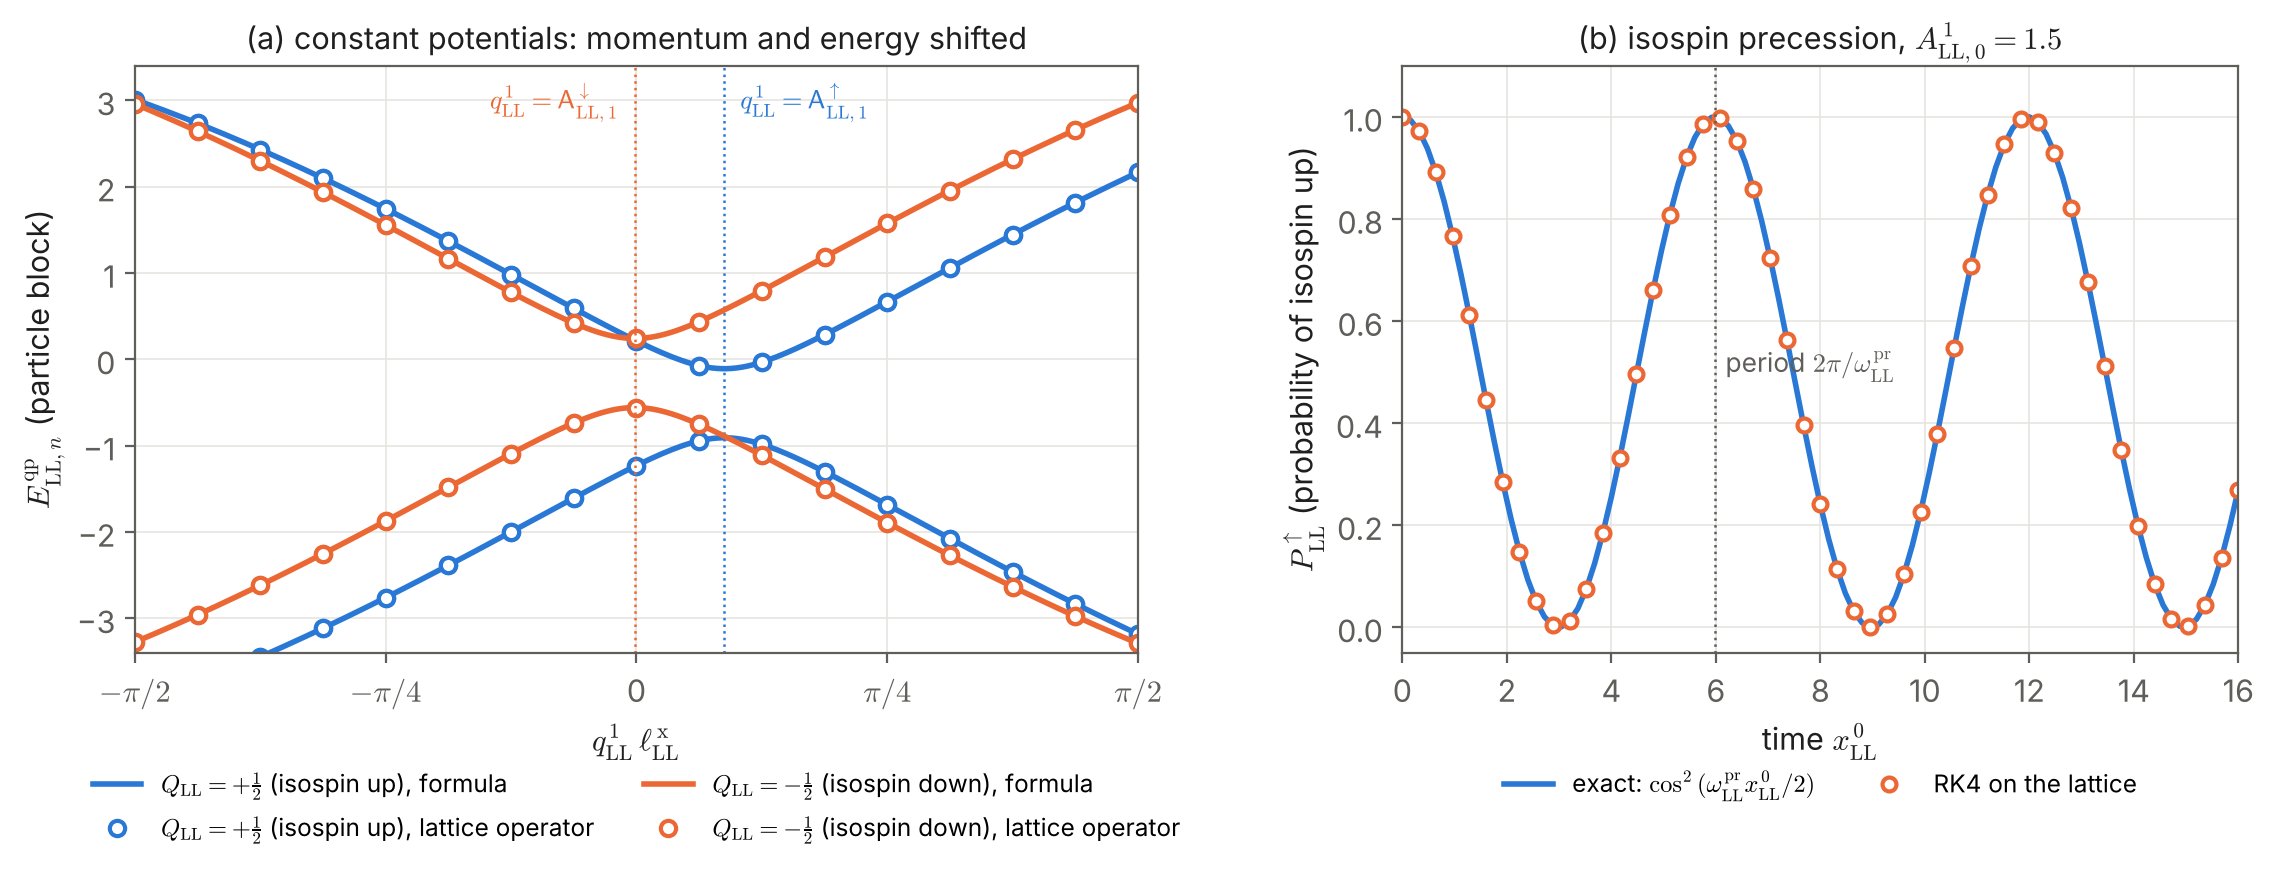
\includegraphics[width=1\textwidth,height=\textheight]{figures/fig_t2_case_A.png}

\textbf{Figure 3.} Case A. (a) The energies of the particle block for
plane waves in the constant potentials \(A^3_{{\rm LL},1}=0.8\),
\(A^{\rm F}_{{\rm LL},1}=0.6\), \(A^3_{{\rm LL},0}=0.5\),
\(A^{\rm F}_{{\rm LL},0}=0.3\) (\(g^{\rm v}_{\rm LL}=0.7\),
\(g^{\rm F}_{\rm LL}=0.45\), \(m_{\rm LL}=0.4\), \(\mu_{\rm LL}=0.2\),
\(\ell^{\rm x}_{\rm LL}=0.5\), \(r^{\rm W}_{\rm LL}=1\)): the curves are
(3.7) with \(\varepsilon^{\rm lat}_{\rm LL}\) for isospin up (blue) and
down (orange); the circles are the eigenvalues of the lattice operator
of the solvers on the plane waves of a ring of 32 sites; the dotted
lines mark the band bottoms at
\(q^1_{\rm LL}=\mathsf A^\uparrow_{{\rm LL},1}=0.55\) and
\(\mathsf A^\downarrow_{{\rm LL},1}=-0.01\). (b) The probability of
isospin up of a particle in the constant isospin potential
\(A^1_{{\rm LL},0}=1.5\): the exact solution (3.8) (line) and the RK4
integration of the lattice equations (circles, every second value
shown), with \(\ell^{\rm t}_{\rm LL}=0.004\). Data:
\texttt{test2/data/t2\_A\_dispersion\_curves.csv},
\texttt{t2\_A\_dispersion\_lattice.csv}, \texttt{t2\_A\_precession.csv}.

\hypertarget{case-b-the-uniform-polar-superfluid}{%
\subsection{3.3 Case B: the uniform polar
superfluid}\label{case-b-the-uniform-polar-superfluid}}

\textbf{The fields.} No gauge fields; a uniform pair field along the
third isospin direction, \(d^\iota_{\rm LL}=(0,0,\Delta_{\rm LL})\) with
a real \(\Delta_{\rm LL}>0\) (the polar state). Then
\(\mathsf P_{\rm LL}=\Delta_{\rm LL}(\mathsf K^3_{\rm LL})^\dagger\) and
\(\mathsf P^\dagger_{\rm LL}=\Delta_{\rm LL}\mathsf K^3_{\rm LL}\). The
pair matrix (Section 2.8) is
\(\mathsf K^3_{\rm LL}=C_{\rm LL}\gamma^{\rm ch}_{\rm LL}\otimes\mathsf E_{\rm LL}\tau^{\rm LL}_3\)
with
\(C_{\rm LL}\gamma^{\rm ch}_{\rm LL}=\mathrm{diag}(-\mathsf E_{\rm LL},-\mathsf E_{\rm LL})\)
and \(\mathsf E_{\rm LL}\tau^{\rm LL}_3=-\tau^{\rm LL}_1\), so

\[\mathsf K^3_{\rm LL}=\begin{pmatrix}0&1&0&0\\-1&0&0&0\\0&0&0&1\\0&0&-1&0\end{pmatrix}\otimes\tau^{\rm LL}_1,\qquad(\mathsf K^3_{\rm LL})^T=(\mathsf K^3_{\rm LL})^\dagger=-\mathsf K^3_{\rm LL},\qquad(\mathsf K^3_{\rm LL})^2=-\mathsf 1_8.\tag{3.10}\]

It is real and unitary.

\textbf{The key identity.} For the plane-wave Hamiltonian
\(\mathsf h_{\rm LL}(\vec q_{\rm LL})=\sum_j\alpha^j_{\rm LL}q^j_{\rm LL}+\beta_{\rm LL}m_{\rm LL}\),

\[\mathsf K^3_{\rm LL}\,\mathsf h_{\rm LL}(\vec q_{\rm LL})=\mathsf h_{\rm LL}(-\vec q_{\rm LL})^*\,\mathsf K^3_{\rm LL}.\tag{3.11}\]

\emph{Proof.} With
\(\alpha^j_{\rm LL}=\mathrm{diag}(-\sigma^{\rm LL}_j,\sigma^{\rm LL}_j)\),
the Dirac factor of \(\mathsf K^3_{\rm LL}\), which is
\(\mathrm{diag}(\mathsf E_{\rm LL},\mathsf E_{\rm LL})\), and the
relation
\(\mathsf E_{\rm LL}\sigma^{\rm LL}_j=-(\sigma^{\rm LL}_j)^*\mathsf E_{\rm LL}\)
(for \(j=1,3\) the Pauli matrix is real and anticommutes with
\(\mathsf E_{\rm LL}=i\sigma^{\rm LL}_2\); for \(j=2\) it commutes with
it and is imaginary), one finds
\(\mathsf K^3_{\rm LL}\alpha^j_{\rm LL}=-(\alpha^j_{\rm LL})^*\mathsf K^3_{\rm LL}\).
The matrix \(\beta_{\rm LL}\) is real and exchanges the two Weyl blocks,
whose Dirac factors are equal, so
\(\mathsf K^3_{\rm LL}\beta_{\rm LL}=\beta_{\rm LL}\mathsf K^3_{\rm LL}\).
Inserted in \(\mathsf h_{\rm LL}\), these give (3.11). It holds on the
lattice as well, with
\(\sin(q^j_{\rm LL}\ell^{\rm x}_{\rm LL})/\ell^{\rm x}_{\rm LL}\) (odd
in \(q^j_{\rm LL}\)) and the Wilson term (even). \(\square\)

\textbf{The Bogoliubov modes.} On plane waves,
\(\mathcal H^{\rm DB}_{\rm LL}(\vec q_{\rm LL})\) has the blocks
\(\mathsf h_{\rm LL}(\vec q_{\rm LL})-\mu_{\rm LL}\),
\(\Delta_{\rm LL}(\mathsf K^3_{\rm LL})^\dagger\),
\(\Delta_{\rm LL}\mathsf K^3_{\rm LL}\) and
\(-(\mathsf h_{\rm LL}(-\vec q_{\rm LL})^*-\mu_{\rm LL})\) (Section
2.10, check GS-8). Let \(\chi^{\rm pw}_{\rm LL}\) be a normalized
eigenvector of \(\mathsf h_{\rm LL}(\vec q_{\rm LL})\) with the
eigenvalue \(+\varepsilon_{\rm LL}\) or \(-\varepsilon_{\rm LL}\)
(\(\varepsilon_{\rm LL}=(q_{\rm LL}^2+m_{\rm LL}^2)^{1/2}\)). By (3.11),
\(\mathsf K^3_{\rm LL}\chi^{\rm pw}_{\rm LL}\) is an eigenvector of
\(\mathsf h_{\rm LL}(-\vec q_{\rm LL})^*\) with the same eigenvalue, and
since \((\mathsf K^3_{\rm LL})^\dagger\mathsf K^3_{\rm LL}=\mathsf 1_8\)
the operator maps the two vectors \((\chi^{\rm pw}_{\rm LL},0)\) and
\((0,\mathsf K^3_{\rm LL}\chi^{\rm pw}_{\rm LL})\) into their span, with
the matrix

\[\begin{pmatrix}\pm\varepsilon_{\rm LL}-\mu_{\rm LL}&\Delta_{\rm LL}\\\Delta_{\rm LL}&-(\pm\varepsilon_{\rm LL}-\mu_{\rm LL})\end{pmatrix}.\tag{3.12}\]

Its square is
\(\big((\pm\varepsilon_{\rm LL}-\mu_{\rm LL})^2+\Delta_{\rm LL}^2\big)\)
times the unit matrix; its eigenvalues are therefore

\[E^{\rm qp}_{{\rm LL},n}=\pm E^-_{\rm LL}\ \text{(from }+\varepsilon_{\rm LL}),\qquad E^{\rm qp}_{{\rm LL},n}=\pm E^+_{\rm LL}\ \text{(from }-\varepsilon_{\rm LL}),\qquad E^\pm_{\rm LL}=\big((\varepsilon_{\rm LL}\pm\mu_{\rm LL})^2+\Delta_{\rm LL}^2\big)^{1/2},\tag{3.13}\]

each four times (the eigenvalue \(+\varepsilon_{\rm LL}\) of the
\(8\times8\) matrix \(\mathsf h_{\rm LL}\) has four eigenvectors, as has
\(-\varepsilon_{\rm LL}\)), and the eigenvector of the positive
eigenvalue is

\[\big(\cos\vartheta^{\rm B}_{\rm LL}\,\chi^{\rm pw}_{\rm LL},\ \sin\vartheta^{\rm B}_{\rm LL}\,\mathsf K^3_{\rm LL}\chi^{\rm pw}_{\rm LL}\big),\qquad\cos^2\vartheta^{\rm B}_{\rm LL}=\tfrac12\Big(1+\frac{\pm\varepsilon_{\rm LL}-\mu_{\rm LL}}{E^\mp_{\rm LL}}\Big),\quad\sin^2\vartheta^{\rm B}_{\rm LL}=\tfrac12\Big(1-\frac{\pm\varepsilon_{\rm LL}-\mu_{\rm LL}}{E^\mp_{\rm LL}}\Big)\tag{3.14}\]

(insert it in (3.12): the first row gives
\(\tan\vartheta^{\rm B}_{\rm LL}=(E^\mp_{\rm LL}-(\pm\varepsilon_{\rm LL}-\mu_{\rm LL}))/\Delta_{\rm LL}\),
the second
\(\tan\vartheta^{\rm B}_{\rm LL}=\Delta_{\rm LL}/(E^\mp_{\rm LL}+(\pm\varepsilon_{\rm LL}-\mu_{\rm LL}))\),
and the two agree because
\((E^\mp_{\rm LL})^2-(\pm\varepsilon_{\rm LL}-\mu_{\rm LL})^2=\Delta_{\rm LL}^2\)).
These are the quasi-particles of the superfluid: a superposition of a
particle and a hole, with the weights
\(\cos^2\vartheta^{\rm B}_{\rm LL}\) and
\(\sin^2\vartheta^{\rm B}_{\rm LL}\). The branch \(E^-_{\rm LL}\) has
its minimum \(\Delta_{\rm LL}\) at the Fermi momentum
\(k^{\rm F}_{\rm LL}\), where \(\varepsilon_{\rm LL}=\mu_{\rm LL}\):
\(\Delta_{\rm LL}\) is the energy gap of the superfluid. The branch
\(E^+_{\rm LL}\) belongs to the states of negative energy (the
antiparticles) and is always above \(\mu_{\rm LL}+m_{\rm LL}\). Check
AS-3 verifies (3.11) to (3.14) for 50 random momenta, chemical
potentials and gaps, and the spectrum (3.13), with
\(\varepsilon^{\rm lat}_{\rm LL}\) in place of \(\varepsilon_{\rm LL}\),
for the lattice operator of the solvers on the plane waves of a ring
(Figure 4(a)).

\textbf{A particle injected into the superfluid oscillates into a hole.}
Start with the particle \((\chi^{\rm pw}_{\rm LL},0)\) of positive
energy \(\varepsilon_{\rm LL}\). Its evolution stays in the plane of
(3.12), where the matrix (3.12) with the upper sign squares to
\((E^-_{\rm LL})^2\) times the unit matrix; its exponential is therefore

\[\exp\Big(-ix^0_{\rm LL}\begin{pmatrix}\varepsilon_{\rm LL}-\mu_{\rm LL}&\Delta_{\rm LL}\\\Delta_{\rm LL}&\mu_{\rm LL}-\varepsilon_{\rm LL}\end{pmatrix}\Big)=\cos(E^-_{\rm LL}x^0_{\rm LL})\begin{pmatrix}1&0\\0&1\end{pmatrix}-\frac{i\sin(E^-_{\rm LL}x^0_{\rm LL})}{E^-_{\rm LL}}\begin{pmatrix}\varepsilon_{\rm LL}-\mu_{\rm LL}&\Delta_{\rm LL}\\\Delta_{\rm LL}&\mu_{\rm LL}-\varepsilon_{\rm LL}\end{pmatrix},\]

and

\[\psi^{\rm p}_{\rm LL}=\Big(\cos(E^-_{\rm LL}x^0_{\rm LL})-i\,\frac{\varepsilon_{\rm LL}-\mu_{\rm LL}}{E^-_{\rm LL}}\sin(E^-_{\rm LL}x^0_{\rm LL})\Big)\chi^{\rm pw}_{\rm LL},\qquad\psi^{\rm h}_{\rm LL}=-i\,\frac{\Delta_{\rm LL}}{E^-_{\rm LL}}\sin(E^-_{\rm LL}x^0_{\rm LL})\,\mathsf K^3_{\rm LL}\chi^{\rm pw}_{\rm LL}\tag{3.15}\]

(both times the plane wave). The probability of the hole is

\[P^{\rm h}_{\rm LL}(x^0_{\rm LL})=\Big(\frac{\Delta_{\rm LL}}{E^-_{\rm LL}}\Big)^2\sin^2(E^-_{\rm LL}x^0_{\rm LL}).\tag{3.16}\]

A bare particle is not a stationary state of the superfluid: the pair
field converts it into a hole and back, with the angular frequency
\(2E^-_{\rm LL}\) and the largest hole probability
\((\Delta_{\rm LL}/E^-_{\rm LL})^2\), which is 1 at the Fermi surface
and small far from it (the Rabi oscillation of a two-state system). This
is the non-conservation of the particle content of a mode found in
(3.2). In the self-consistent state the fermion number is nevertheless
conserved, (3.3). Figure 4(b) and check AS-4: the RK4 integration of the
lattice equations agrees with (3.15) to \(5\times10^{-10}\), the
predicted size of the RK4 phase error.

\textbf{The gap equation in closed form.} For massless spinor charges
(\(m_{\rm LL}=0\), \(\varepsilon_{\rm LL}=q_{\rm LL}\)) the integral of
(2.33) can be done. With
\(d^3q_{\rm LL}/(2\pi)^3=q_{\rm LL}^2\,dq_{\rm LL}/(2\pi^2)\) for an
integrand that depends only on \(q_{\rm LL}\), one needs antiderivatives
of \(q_{\rm LL}^2/E^\pm_{\rm LL}\). They are

\[\frac{d}{dq_{\rm LL}}\Big[\tfrac12(q_{\rm LL}\mp3\mu_{\rm LL})E^\pm_{\rm LL}+(\mu_{\rm LL}^2-\tfrac12\Delta_{\rm LL}^2)\,\mathrm{arsinh}\frac{q_{\rm LL}\pm\mu_{\rm LL}}{\Delta_{\rm LL}}\Big]=\frac{q_{\rm LL}^2}{E^\pm_{\rm LL}},\]

as one verifies by differentiating: the derivative of the bracket,
multiplied by \(E^\pm_{\rm LL}\), is
\(\tfrac12(E^\pm_{\rm LL})^2+\tfrac12(q_{\rm LL}\mp3\mu_{\rm LL})(q_{\rm LL}\pm\mu_{\rm LL})+\mu_{\rm LL}^2-\tfrac12\Delta_{\rm LL}^2=q_{\rm LL}^2\).
At \(q_{\rm LL}=0\) the two brackets cancel each other
(\(E^+_{\rm LL}=E^-_{\rm LL}\) there, and \(\mathrm{arsinh}\) is odd),
so

\[\begin{aligned}\frac1{G_{\rm LL}}=\frac1{4\pi^2}\Big[&(\Lambda_{\rm LL}-3\mu_{\rm LL})E^+_{\rm LL}(\Lambda_{\rm LL})+(\Lambda_{\rm LL}+3\mu_{\rm LL})E^-_{\rm LL}(\Lambda_{\rm LL})\\&+(2\mu_{\rm LL}^2-\Delta_{\rm LL}^2)\Big(\mathrm{arsinh}\frac{\Lambda_{\rm LL}+\mu_{\rm LL}}{\Delta_{\rm LL}}+\mathrm{arsinh}\frac{\Lambda_{\rm LL}-\mu_{\rm LL}}{\Delta_{\rm LL}}\Big)\Big],\end{aligned}\tag{3.17}\]

with
\(E^\pm_{\rm LL}(\Lambda_{\rm LL})=((\Lambda_{\rm LL}\pm\mu_{\rm LL})^2+\Delta_{\rm LL}^2)^{1/2}\).
At \(\mu_{\rm LL}=0\),

\[\frac1{G_{\rm LL}}=\frac1{2\pi^2}\Big[\Lambda_{\rm LL}(\Lambda_{\rm LL}^2+\Delta_{\rm LL}^2)^{1/2}-\Delta_{\rm LL}^2\,\mathrm{arsinh}\frac{\Lambda_{\rm LL}}{\Delta_{\rm LL}}\Big],\qquad G^{\rm crit}_{\rm LL}=\frac{2\pi^2}{\Lambda_{\rm LL}^2}.\tag{3.18}\]

The right side of (3.18) decreases from \(\Lambda_{\rm LL}^2/(2\pi^2)\)
as \(\Delta_{\rm LL}\) grows (the integrand of (2.33) decreases with
\(\Delta_{\rm LL}\)), so at \(\mu_{\rm LL}=0\) a gap exists only for
\(G_{\rm LL}>G^{\rm crit}_{\rm LL}\): below the critical coupling the
vacuum stays normal, above it the vacuum itself condenses. Near the
critical coupling, the expansions
\(\Lambda_{\rm LL}(\Lambda_{\rm LL}^2+\Delta_{\rm LL}^2)^{1/2}\approx\Lambda_{\rm LL}^2+\tfrac12\Delta_{\rm LL}^2\)
and
\(\mathrm{arsinh}(\Lambda_{\rm LL}/\Delta_{\rm LL})\approx\ln(2\Lambda_{\rm LL}/\Delta_{\rm LL})\)
give

\[\Delta_{\rm LL}^2\Big(\ln\frac{2\Lambda_{\rm LL}}{\Delta_{\rm LL}}-\frac12\Big)\approx2\pi^2\Big(\frac1{G^{\rm crit}_{\rm LL}}-\frac1{G_{\rm LL}}\Big):\tag{3.19}\]

the gap grows continuously from zero. For \(\mu_{\rm LL}>0\) the
situation is different: as \(\Delta_{\rm LL}\to0\) the arsinh terms of
(3.17) grow like \(\ln(1/\Delta_{\rm LL})\) with the coefficient
\(2\mu_{\rm LL}^2\) (the Fermi surface), so a solution exists for every
attractive coupling. With
\(E^\pm_{\rm LL}(\Lambda_{\rm LL})\to\Lambda_{\rm LL}\pm\mu_{\rm LL}\)
and
\(\mathrm{arsinh}((\Lambda_{\rm LL}\pm\mu_{\rm LL})/\Delta_{\rm LL})\to\ln(2(\Lambda_{\rm LL}\pm\mu_{\rm LL})/\Delta_{\rm LL})\),
(3.17) becomes
\(1/G_{\rm LL}=(\Lambda_{\rm LL}^2-3\mu_{\rm LL}^2+\mu_{\rm LL}^2\ln(4(\Lambda_{\rm LL}^2-\mu_{\rm LL}^2)/\Delta_{\rm LL}^2))/(2\pi^2)\),
whose solution is the weak-coupling (BCS) gap

\[\begin{aligned}\Delta_{\rm LL}&=2(\Lambda_{\rm LL}^2-\mu_{\rm LL}^2)^{1/2}\exp(-\tfrac32)\exp\Big(-\frac{\pi^2}{\mu_{\rm LL}^2}\Big(\frac1{G_{\rm LL}}-\frac1{G^{\rm crit}_{\rm LL}}\Big)\Big)\\&=2(\Lambda_{\rm LL}^2-\mu_{\rm LL}^2)^{1/2}\exp(-\tfrac32)\exp\Big(-\frac1{2\nu^{\rm F}_{\rm LL}}\Big(\frac1{G_{\rm LL}}-\frac1{G^{\rm crit}_{\rm LL}}\Big)\Big),\end{aligned}\tag{3.20}\]

with the density of states
\(\nu^{\rm F}_{\rm LL}=\mu_{\rm LL}^2/(2\pi^2)\) of massless charges at
the Fermi surface (\(k^{\rm F}_{\rm LL}=\mu_{\rm LL}\)): exponentially
small, as in the theory of Bardeen, Cooper and Schrieffer. The neglected
terms of (3.17) are of the order
\(\Delta_{\rm LL}^2\ln(\Lambda_{\rm LL}/\Delta_{\rm LL})\) (from the
factor \(2\mu_{\rm LL}^2-\Delta_{\rm LL}^2\)); carried through the
solution, they make the relative error of (3.20) equal to
\(-(\Delta_{\rm LL}^2/(2\mu_{\rm LL}^2))\ln(\Lambda_{\rm LL}/\Delta_{\rm LL})\)
to leading order. Check AS-5 verifies (3.17) against numerical
quadrature (to \(2\times10^{-15}\)), \(G^{\rm crit}_{\rm LL}\), the
solutions of (3.17) by bisection, and (3.20) together with its error
term; Figure 4(c) shows \(\Delta_{\rm LL}\) as a function of
\(G_{\rm LL}\) for three chemical potentials.

\textbf{The uniform state is an exact self-consistent solution on the
lattice.} On a periodic chain of \(n^{\rm x}_{\rm LL}\) sites (one
active direction), the eigenvectors of the lattice operator are unit
vectors; the mode functions of the normalization of (2.32) are these
components divided by \((\ell^{\rm x}_{\rm LL})^{1/2}\). Summed over the
positive-energy modes, the pair expectation of (2.32) at each site is
\(-2\Delta_{\rm LL}(n^{\rm x}_{\rm LL}\ell^{\rm x}_{\rm LL})^{-1}\sum_{q^1_{\rm LL}}(1/E^+_{\rm LL}+1/E^-_{\rm LL})\)
for \(\iota=3\) and 0 for \(\iota=1,2\) (the lattice form of check GS-9;
the sum runs over the \(n^{\rm x}_{\rm LL}\) allowed momenta, with
\(\varepsilon^{\rm lat}_{\rm LL}\) in \(E^\pm_{\rm LL}\)). The
self-consistency condition (2.32) therefore returns the same pair field
\(d^\iota_{\rm LL}=(0,0,\Delta_{\rm LL})\) on every site exactly when

\[\frac1{G_{\rm LL}}=\frac1{n^{\rm x}_{\rm LL}\ell^{\rm x}_{\rm LL}}\sum_{q^1_{\rm LL}}\Big(\frac1{E^+_{\rm LL}}+\frac1{E^-_{\rm LL}}\Big),\tag{3.21}\]

the gap equation of the lattice chain (the integral
\(\int dq^1_{\rm LL}/(2\pi)\) of a one-dimensional problem replaced by
the sum over the allowed momenta divided by the circumference). Check
AS-6 computes the pair expectation with the routine of the solvers from
the 128 positive-energy eigenvectors of a chain of 16 sites
(\(\mu_{\rm LL}=0.6\), \(\Delta_{\rm LL}=0.3\)) and finds (3.21) and the
fixed point to \(10^{-15}\): a known fixed point for the self-consistent
solvers of items {[}3{]} and {[}5{]}.

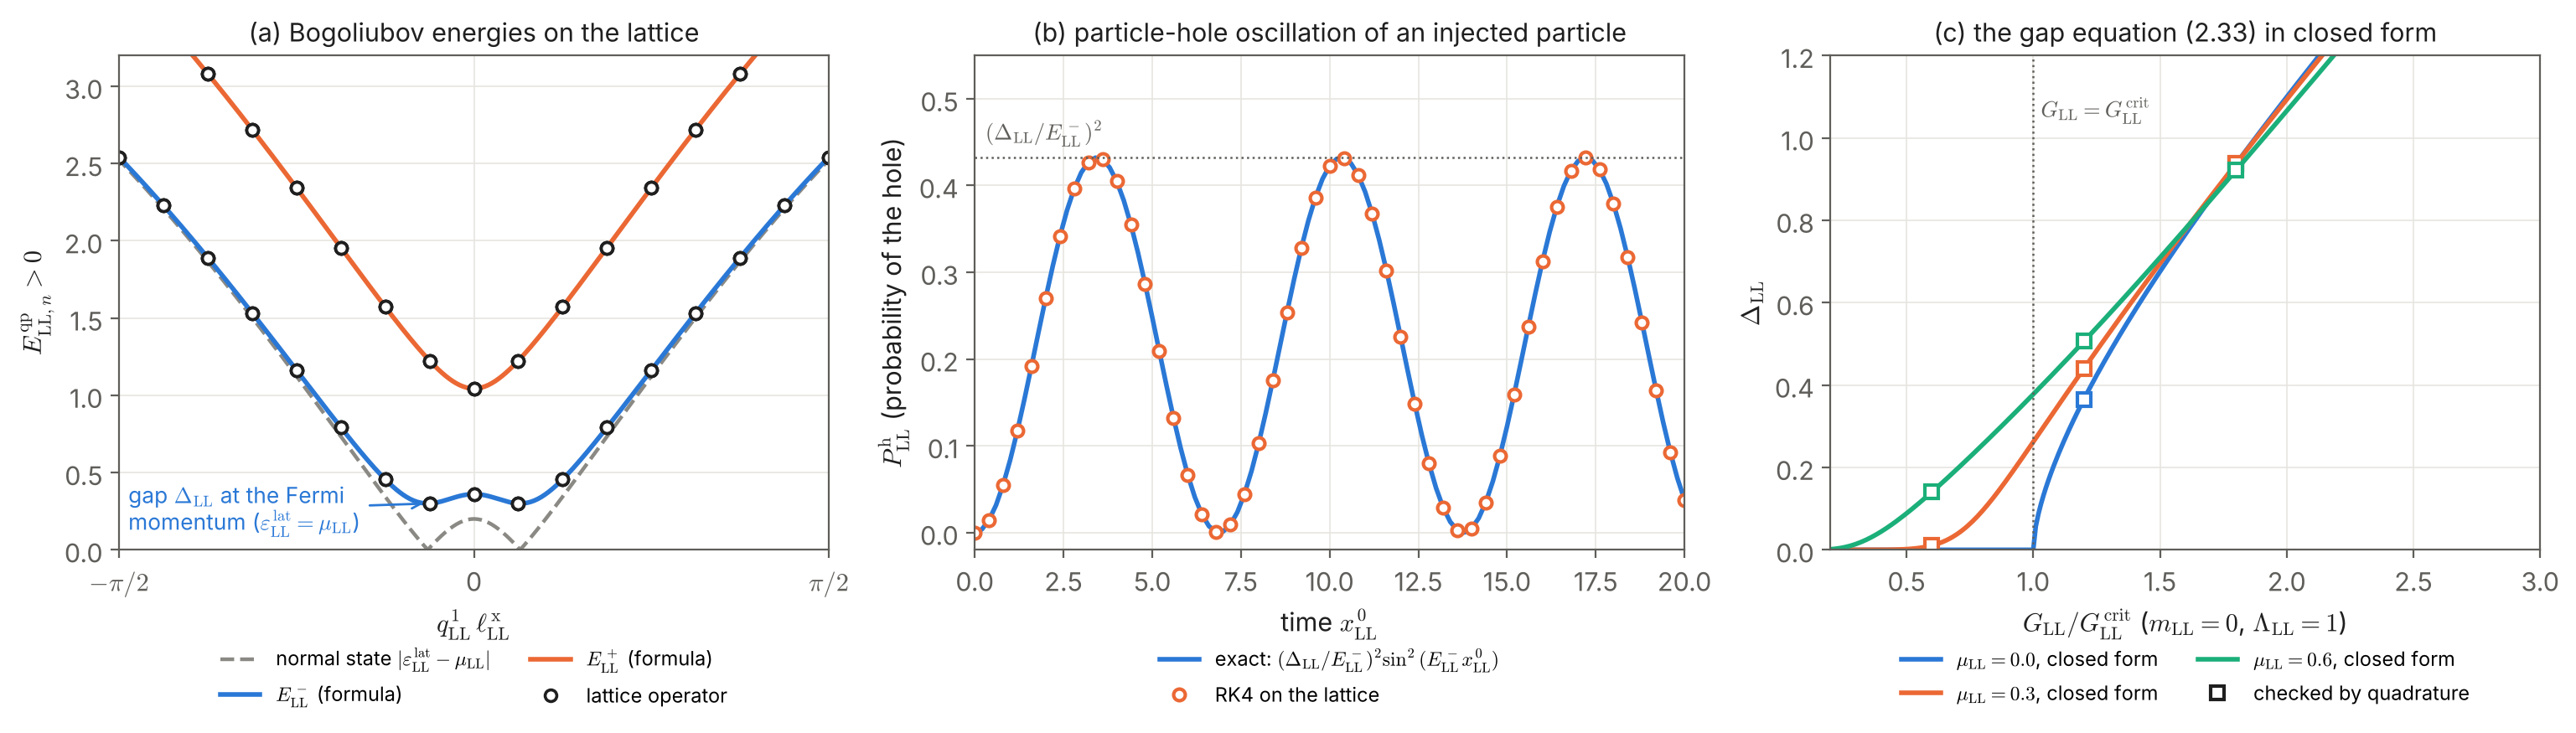
\includegraphics[width=1\textwidth,height=\textheight]{figures/fig_t2_case_B.png}

\textbf{Figure 4.} Case B, the uniform polar superfluid. (a) The
positive energies on the lattice (\(m_{\rm LL}=0.4\),
\(\mu_{\rm LL}=0.6\), \(\Delta_{\rm LL}=0.3\),
\(\ell^{\rm x}_{\rm LL}=0.5\), \(r^{\rm W}_{\rm LL}=1\)):
\(E^-_{\rm LL}\) (blue) and \(E^+_{\rm LL}\) (orange) from (3.13) with
\(\varepsilon^{\rm lat}_{\rm LL}\), the normal-state energy
\(\lvert\varepsilon^{\rm lat}_{\rm LL}-\mu_{\rm LL}\rvert\) (grey,
dashed), and the eigenvalues of the lattice operator of the solvers on
the plane waves of a ring of 32 sites (circles); the gap
\(\Delta_{\rm LL}\) opens at the Fermi momentum. (b) The probability of
the hole of a particle injected at the momentum
\(2\pi/(16\ell^{\rm x}_{\rm LL})\): (3.16) (line) and the RK4
integration of the lattice equations (circles, every second value),
\(\ell^{\rm t}_{\rm LL}=0.02\). (c) The gap as a function of the
coupling for massless charges (\(\Lambda_{\rm LL}=1\)) at
\(\mu_{\rm LL}=0\), \(0.3\) and \(0.6\): the solutions of the closed
form (3.17) (lines) and their check by numerical quadrature (squares).
At \(\mu_{\rm LL}=0\) the gap appears at \(G^{\rm crit}_{\rm LL}\); at
\(\mu_{\rm LL}>0\) it is non-zero for every coupling, exponentially
small at weak coupling (3.20). Data:
\texttt{test2/data/t2\_B\_bogoliubov\_curves.csv},
\texttt{t2\_B\_bogoliubov\_lattice.csv}, \texttt{t2\_B\_rabi.csv},
\texttt{t2\_B\_gap.csv}.

\hypertarget{case-c-a-domain-wall-of-the-pair-field}{%
\subsection{3.4 Case C: a domain wall of the pair
field}\label{case-c-a-domain-wall-of-the-pair-field}}

\textbf{The fields.} No gauge fields, \(\mu_{\rm LL}=0\), and a real
pair field along the third isospin direction that depends on
\(x^1_{\rm LL}\) and changes sign:

\[d^\iota_{\rm LL}=(0,0,\Delta_{\rm LL}(x^1_{\rm LL})),\qquad\Delta_{\rm LL}(x^1_{\rm LL})=\Delta^\infty_{\rm LL}\tanh(x^1_{\rm LL}/\ell^{\rm K}_{\rm LL}).\tag{3.22}\]

Two superfluid domains with opposite signs of the order parameter (a
phase difference \(\pi\)) meet at a wall of the width
\(\ell^{\rm K}_{\rm LL}\) (a kink). The fields do not depend on
\(x^2_{\rm LL}\), \(x^3_{\rm LL}\), and the modes are taken as plane
waves \(\exp(i(q^2_{\rm LL}x^2_{\rm LL}+q^3_{\rm LL}x^3_{\rm LL}))\)
along the wall; first \(q^2_{\rm LL}=q^3_{\rm LL}=0\).

\textbf{Four matrix facts.} With (3.10) and
\(\alpha^1_{\rm LL}=\mathrm{diag}(-\sigma^{\rm LL}_1,\sigma^{\rm LL}_1)\):

\[\big((\mathsf K^3_{\rm LL})^\dagger\big)^2=-\mathsf 1_8,\qquad\alpha^1_{\rm LL}(\mathsf K^3_{\rm LL})^\dagger\alpha^1_{\rm LL}=-(\mathsf K^3_{\rm LL})^\dagger,\qquad\beta_{\rm LL}(\mathsf K^3_{\rm LL})^\dagger\alpha^1_{\rm LL}=-(\mathsf K^3_{\rm LL})^\dagger\alpha^1_{\rm LL}\beta_{\rm LL},\qquad\alpha^1_{\rm LL},\ \beta_{\rm LL}\ \text{real}.\tag{3.23}\]

The second follows from
\(\sigma^{\rm LL}_1\mathsf E_{\rm LL}\sigma^{\rm LL}_1=-\mathsf E_{\rm LL}\),
the third from the second and
\(\alpha^1_{\rm LL}\beta_{\rm LL}=-\beta_{\rm LL}\alpha^1_{\rm LL}\),
\(\beta_{\rm LL}(\mathsf K^3_{\rm LL})^\dagger=(\mathsf K^3_{\rm LL})^\dagger\beta_{\rm LL}\).

\textbf{The bound states.} Let \(\varphi^{\rm K}_{\rm LL}\) solve
\(d\varphi^{\rm K}_{\rm LL}/dx^1_{\rm LL}=-\Delta_{\rm LL}\varphi^{\rm K}_{\rm LL}\),
that is
\(\varphi^{\rm K}_{\rm LL}(x^1_{\rm LL})=\cosh(x^1_{\rm LL}/\ell^{\rm K}_{\rm LL})^{-\Delta^\infty_{\rm LL}\ell^{\rm K}_{\rm LL}}\)
for the kink (3.22), and let \(\chi^{\rm K}_{\rm LL}\) be a constant
8-component spinor with
\(\beta_{\rm LL}\chi^{\rm K}_{\rm LL}=\pm\chi^{\rm K}_{\rm LL}\). Then

\[\psi^{\rm p}_{\rm LL}=\varphi^{\rm K}_{\rm LL}\chi^{\rm K}_{\rm LL},\qquad\psi^{\rm h}_{\rm LL}=i(\mathsf K^3_{\rm LL})^\dagger\alpha^1_{\rm LL}\varphi^{\rm K}_{\rm LL}\chi^{\rm K}_{\rm LL},\qquad E^{\rm qp}_{{\rm LL},n}=\pm m_{\rm LL}\tag{3.24}\]

is a stationary solution of (3.1). \emph{Proof.} Particle row:
\(-i\alpha^1_{\rm LL}\partial_1\psi^{\rm p}_{\rm LL}+\beta_{\rm LL}m_{\rm LL}\psi^{\rm p}_{\rm LL}+\Delta_{\rm LL}(\mathsf K^3_{\rm LL})^\dagger\psi^{\rm h}_{\rm LL} =i\Delta_{\rm LL}\varphi^{\rm K}_{\rm LL}\alpha^1_{\rm LL}\chi^{\rm K}_{\rm LL}\pm m_{\rm LL}\varphi^{\rm K}_{\rm LL}\chi^{\rm K}_{\rm LL}+i\Delta_{\rm LL}\varphi^{\rm K}_{\rm LL}\big((\mathsf K^3_{\rm LL})^\dagger\big)^2\alpha^1_{\rm LL}\chi^{\rm K}_{\rm LL}=\pm m_{\rm LL}\psi^{\rm p}_{\rm LL}\)
by the first fact. Hole row (with
\(\mathsf P^\dagger_{\rm LL}=\Delta_{\rm LL}\mathsf K^3_{\rm LL}=-\Delta_{\rm LL}(\mathsf K^3_{\rm LL})^\dagger\)
and the real matrices):
\(\Delta_{\rm LL}\mathsf K^3_{\rm LL}\psi^{\rm p}_{\rm LL}-(i\alpha^1_{\rm LL}\partial_1+\beta_{\rm LL}m_{\rm LL})\psi^{\rm h}_{\rm LL} =-\Delta_{\rm LL}\varphi^{\rm K}_{\rm LL}(\mathsf K^3_{\rm LL})^\dagger\chi^{\rm K}_{\rm LL}-\Delta_{\rm LL}\varphi^{\rm K}_{\rm LL}\alpha^1_{\rm LL}(\mathsf K^3_{\rm LL})^\dagger\alpha^1_{\rm LL}\chi^{\rm K}_{\rm LL}-im_{\rm LL}\varphi^{\rm K}_{\rm LL}\beta_{\rm LL}(\mathsf K^3_{\rm LL})^\dagger\alpha^1_{\rm LL}\chi^{\rm K}_{\rm LL}\);
the first two terms cancel by the second fact, and the third is
\(im_{\rm LL}\varphi^{\rm K}_{\rm LL}(\mathsf K^3_{\rm LL})^\dagger\alpha^1_{\rm LL}\beta_{\rm LL}\chi^{\rm K}_{\rm LL}=\pm m_{\rm LL}\psi^{\rm h}_{\rm LL}\)
by the third. \(\square\)

The profile decays like
\(\exp(-\Delta^\infty_{\rm LL}\lvert x^1_{\rm LL}\rvert)\) on both
sides, because \(\Delta_{\rm LL}\) has opposite signs on the two sides;
the state is bound to the wall. The eigenspaces \(\beta_{\rm LL}=+1\)
and \(\beta_{\rm LL}=-1\) of the 8-component spinors are
four-dimensional each, so every wall carries four bound states at
\(+m_{\rm LL}\) and four at \(-m_{\rm LL}\) (for massless charges, eight
zero modes). Their energy does not depend on the shape of the profile,
only on the change of sign; this is the mechanism of Jackiw and Rebbi,
here for the pair field of the spinor charges (and the relativistic
counterpart of the bound states of a superconductor with a phase jump
\(\pi\)). For an antikink,
\(\Delta_{\rm LL}=-\Delta^\infty_{\rm LL}\tanh(x^1_{\rm LL}/\ell^{\rm K}_{\rm LL})\),
the bound states are
\(\psi^{\rm p}_{\rm LL}=\varphi^{\rm K}_{\rm LL}\chi^{\rm K}_{\rm LL}\),
\(\psi^{\rm h}_{\rm LL}=-i(\mathsf K^3_{\rm LL})^\dagger\alpha^1_{\rm LL}\varphi^{\rm K}_{\rm LL}\chi^{\rm K}_{\rm LL}\)
with the same profile and the same energies, by the same steps with
\(\Delta_{\rm LL}\) replaced by \(-\Delta_{\rm LL}\). Check AS-7
verifies (3.23) and (3.24) at 50 random points with random spinors.

\textbf{The square of the operator, and all bound states.} With the
plane wave
\(\exp(i(q^2_{\rm LL}x^2_{\rm LL}+q^3_{\rm LL}x^3_{\rm LL}))\) along the
wall, the particle block of \(\mathcal H^{\rm DB}_{\rm LL}\) is the
operator
\(-i\alpha^1_{\rm LL}\partial_1+\alpha^2_{\rm LL}q^2_{\rm LL}+\alpha^3_{\rm LL}q^3_{\rm LL}+\beta_{\rm LL}m_{\rm LL}\)
and the hole block is
\(-(i(\alpha^1_{\rm LL})^*\partial_1-(\alpha^2_{\rm LL})^*q^2_{\rm LL}-(\alpha^3_{\rm LL})^*q^3_{\rm LL}+\beta_{\rm LL}m_{\rm LL})\).
By the relation
\(\alpha^j_{\rm LL}(\mathsf K^3_{\rm LL})^\dagger=-(\mathsf K^3_{\rm LL})^\dagger(\alpha^j_{\rm LL})^*\)
(all \(j\); it is (3.11) in another form) the particle block times
\((\mathsf K^3_{\rm LL})^\dagger\) equals
\((\mathsf K^3_{\rm LL})^\dagger\) times the hole operator without its
minus sign, so in the off-diagonal blocks of
\((\mathcal H^{\rm DB}_{\rm LL})^2\) everything cancels except the
derivative of \(\Delta_{\rm LL}\), which comes from \(\partial_1\)
acting on the factor \(\Delta_{\rm LL}\). The diagonal blocks are the
squares of the particle and hole operators plus
\(\Delta_{\rm LL}^2(\mathsf K^3_{\rm LL})^\dagger\mathsf K^3_{\rm LL}=\Delta_{\rm LL}^2\mathsf 1_8\).
The result is

\[(\mathcal H^{\rm DB}_{\rm LL})^2=-\frac{d^2}{d(x^1_{\rm LL})^2}+(q^2_{\rm LL})^2+(q^3_{\rm LL})^2+m_{\rm LL}^2+\Delta_{\rm LL}^2+\frac{d\Delta_{\rm LL}}{dx^1_{\rm LL}}\,\mathsf Q^{\rm K}_{\rm LL},\qquad\mathsf Q^{\rm K}_{\rm LL}=\begin{pmatrix}0&-i\alpha^1_{\rm LL}(\mathsf K^3_{\rm LL})^\dagger\\-i\alpha^1_{\rm LL}\mathsf K^3_{\rm LL}&0\end{pmatrix},\tag{3.25}\]

where the scalar terms multiply the \(16\times16\) unit matrix. The
constant matrix \(\mathsf Q^{\rm K}_{\rm LL}\) is Hermitian, its square
is the unit matrix, and its trace is 0: it has the eigenvalue \(-1\) on
an eight-dimensional subspace and \(+1\) on another. On these subspaces
(3.25) is \(m_{\rm LL}^2+(q^2_{\rm LL})^2+(q^3_{\rm LL})^2\) plus one of
the two scalar operators

\[\begin{aligned}\Big(-\frac{d}{dx^1_{\rm LL}}+\Delta_{\rm LL}\Big)\Big(\frac{d}{dx^1_{\rm LL}}+\Delta_{\rm LL}\Big)&=-\frac{d^2}{d(x^1_{\rm LL})^2}+\Delta_{\rm LL}^2-\frac{d\Delta_{\rm LL}}{dx^1_{\rm LL}}\qquad(\mathsf Q^{\rm K}_{\rm LL}=-1),\\\Big(\frac{d}{dx^1_{\rm LL}}+\Delta_{\rm LL}\Big)\Big(-\frac{d}{dx^1_{\rm LL}}+\Delta_{\rm LL}\Big)&=-\frac{d^2}{d(x^1_{\rm LL})^2}+\Delta_{\rm LL}^2+\frac{d\Delta_{\rm LL}}{dx^1_{\rm LL}}\qquad(\mathsf Q^{\rm K}_{\rm LL}=+1).\end{aligned}\tag{3.26}\]

The two operators are products of the same first-order operator and its
adjoint in the two orders. Such products have the same non-zero
eigenvalues (if one of them maps a function to a multiple of itself,
applying the first-order factor gives an eigenfunction of the other with
the same eigenvalue). They differ only in the zero eigenvalue:
\((d/dx^1_{\rm LL}+\Delta_{\rm LL})\varphi^{\rm K}_{\rm LL}=0\) with the
normalizable profile \(\varphi^{\rm K}_{\rm LL}\), while the solutions
of the first-order equation with \(-d/dx^1_{\rm LL}+\Delta_{\rm LL}\) in
place of \(d/dx^1_{\rm LL}+\Delta_{\rm LL}\) are the multiples of
\(1/\varphi^{\rm K}_{\rm LL}\), which grow on both sides. So the sector
\(\mathsf Q^{\rm K}_{\rm LL}=-1\) has exactly one bound state more than
the sector \(\mathsf Q^{\rm K}_{\rm LL}=+1\): the state (3.24), with
\((E^{\rm qp}_{{\rm LL},n})^2=m_{\rm LL}^2+(q^2_{\rm LL})^2+(q^3_{\rm LL})^2\).
For any profile with a sign change this pairing fixes the one unpaired
level (an index theorem); its energy

\[E^{\rm qp}_{{\rm LL},n}=\pm\big(m_{\rm LL}^2+(q^2_{\rm LL})^2+(q^3_{\rm LL})^2\big)^{1/2}\tag{3.27}\]

is that of a free Dirac particle of the mass \(m_{\rm LL}\) moving in
the two dimensions of the wall: the wall carries a \((2+1)\)-dimensional
spinor field.

For the kink (3.22),
\(\Delta_{\rm LL}^2\mp d\Delta_{\rm LL}/dx^1_{\rm LL}=(\Delta^\infty_{\rm LL})^2-\Delta^\infty_{\rm LL}(\Delta^\infty_{\rm LL}\pm1/\ell^{\rm K}_{\rm LL})\cosh(x^1_{\rm LL}/\ell^{\rm K}_{\rm LL})^{-2}\)
(use \(\tanh^2=1-\cosh^{-2}\) and
\(d\tanh(x^1_{\rm LL}/\ell^{\rm K}_{\rm LL})/dx^1_{\rm LL}=\cosh(x^1_{\rm LL}/\ell^{\rm K}_{\rm LL})^{-2}/\ell^{\rm K}_{\rm LL}\)):
so the operator of the sector \(\mathsf Q^{\rm K}_{\rm LL}=-1\) is
\((\Delta^\infty_{\rm LL})^2\) plus the well
\(-d^2/d(x^1_{\rm LL})^2-\Delta^\infty_{\rm LL}(\Delta^\infty_{\rm LL}+1/\ell^{\rm K}_{\rm LL})\cosh(x^1_{\rm LL}/\ell^{\rm K}_{\rm LL})^{-2}\)
(a well of the Pöschl-Teller form, with the parameter
\(\Delta^\infty_{\rm LL}\)), and the operator of the sector \(+1\) is
\((\Delta^\infty_{\rm LL})^2\) plus the same kind of well with the
parameter \(\Delta^\infty_{\rm LL}-1/\ell^{\rm K}_{\rm LL}\), because
\((\Delta^\infty_{\rm LL}-1/\ell^{\rm K}_{\rm LL})(\Delta^\infty_{\rm LL}-1/\ell^{\rm K}_{\rm LL}+1/\ell^{\rm K}_{\rm LL})=\Delta^\infty_{\rm LL}(\Delta^\infty_{\rm LL}-1/\ell^{\rm K}_{\rm LL})\).
By the pairing argument above, the well with the parameter
\(\Delta^\infty_{\rm LL}\) has one bound state more than the well with
the parameter \(\Delta^\infty_{\rm LL}-1/\ell^{\rm K}_{\rm LL}\): the
state
\(\cosh(x^1_{\rm LL}/\ell^{\rm K}_{\rm LL})^{-\Delta^\infty_{\rm LL}\ell^{\rm K}_{\rm LL}}\),
with the eigenvalue \(-(\Delta^\infty_{\rm LL})^2\) of the well; all its
other bound states are those of the well with the smaller parameter.
Applying this repeatedly, as long as the parameter stays positive, gives
the eigenvalues
\(-(\Delta^\infty_{\rm LL}-k^{\rm K}_{\rm LL}/\ell^{\rm K}_{\rm LL})^2\)
of the well with the parameter \(\Delta^\infty_{\rm LL}\), for the
integers
\(0\le k^{\rm K}_{\rm LL}<\Delta^\infty_{\rm LL}\ell^{\rm K}_{\rm LL}\),
and those with
\(1\le k^{\rm K}_{\rm LL}<\Delta^\infty_{\rm LL}\ell^{\rm K}_{\rm LL}\)
for the sector \(+1\). Adding
\((\Delta^\infty_{\rm LL})^2+m_{\rm LL}^2+(q^2_{\rm LL})^2+(q^3_{\rm LL})^2\),
the bound states of the wall are

\[E^{\rm qp}_{{\rm LL},n}=\pm\Big(m_{\rm LL}^2+(q^2_{\rm LL})^2+(q^3_{\rm LL})^2+\frac{2k^{\rm K}_{\rm LL}\Delta^\infty_{\rm LL}}{\ell^{\rm K}_{\rm LL}}-\frac{(k^{\rm K}_{\rm LL})^2}{(\ell^{\rm K}_{\rm LL})^2}\Big)^{1/2},\qquad k^{\rm K}_{\rm LL}=0,1,2,\dots,\ k^{\rm K}_{\rm LL}<\Delta^\infty_{\rm LL}\ell^{\rm K}_{\rm LL},\tag{3.28}\]

four times each sign for \(k^{\rm K}_{\rm LL}=0\) (the sector
\(\mathsf Q^{\rm K}_{\rm LL}=-1\) only) and eight times each sign for
\(k^{\rm K}_{\rm LL}\ge1\) (both sectors); the continuum begins at
\(m_{\rm LL}^2+(q^2_{\rm LL})^2+(q^3_{\rm LL})^2+(\Delta^\infty_{\rm LL})^2\).
In particular, for \(\Delta^\infty_{\rm LL}\ell^{\rm K}_{\rm LL}\le1\)
the states (3.24) are the only bound states. Check AS-8 verifies (3.25)
by applying the operator twice to a Gaussian times a random 16-component
vector (with exact derivatives, for 50 random kinks, points and
momenta), the properties of \(\mathsf Q^{\rm K}_{\rm LL}\), and the
bound states of the two scalar operators (3.26) by finite differences
for \(\Delta^\infty_{\rm LL}\ell^{\rm K}_{\rm LL}=1\) and \(2.5\) (one
and zero, and three and two bound states).

\textbf{On the lattice: sixteen bound states, and the first-order effect
of the Wilson term.} A periodic lattice needs a second wall; the checks
use a ring of length 24 with a kink at \(x^1_{\rm LL}=6\) and an
antikink at \(x^1_{\rm LL}=18\),
\(\Delta_{\rm LL}=\tanh(x^1_{\rm LL}-6)\tanh(18-x^1_{\rm LL})\)
(\(\Delta^\infty_{\rm LL}=\ell^{\rm K}_{\rm LL}=1\), so by (3.28) only
the states (3.24) are bound), \(m_{\rm LL}=0.4\),
\(r^{\rm W}_{\rm LL}=1\). On 60 sites (\(\ell^{\rm x}_{\rm LL}=0.4\))
the lattice operator has exactly 16 eigenvalues inside the gap of the
continuum, eight near \(+m_{\rm LL}\) and eight near \(-m_{\rm LL}\)
(four per wall and sign), and their density sits on the two walls with
the profile \((\varphi^{\rm K}_{\rm LL})^2\) (Figure 5(a) to (c)). They
lie slightly above \(m_{\rm LL}\) in magnitude, by the Wilson term. To
see by how much, insert the analytic state (3.24) on the lattice, with
the spinor \(\chi^{\rm K}_{\rm LL}\) whose components 1 and 5 are
\(1/\sqrt2\) and whose other components are zero
(\(\beta_{\rm LL}\chi^{\rm K}_{\rm LL}=\chi^{\rm K}_{\rm LL}\), because
\(\beta_{\rm LL}\) exchanges the Dirac components 1 and 3, which are the
components 1 and 5 of the field), and compute its Rayleigh quotient
\(E^{\rm R}_{\rm LL}\). In
\((\mathcal H^{\rm lat}_{\rm LL}-m_{\rm LL})\) applied to the state, the
mass terms cancel as in the proof of (3.24); the terms with
\(\alpha^1_{\rm LL}\) and the pair field contribute nothing to the
Rayleigh quotient, because
\((\chi^{\rm K}_{\rm LL})^\dagger\alpha^1_{\rm LL}\chi^{\rm K}_{\rm LL}=0\)
for an eigenvector of \(\beta_{\rm LL}\) (which anticommutes with
\(\alpha^1_{\rm LL}\)); the Wilson terms of the particle and of the hole
part add. With a summation by parts on the ring,

\[\begin{aligned}E^{\rm R}_{\rm LL}&=m_{\rm LL}+\frac{r^{\rm W}_{\rm LL}}{2\ell^{\rm x}_{\rm LL}}\,\frac{\sum_{s^1_{\rm LL}}\big(\varphi^{\rm K}_{\rm LL}((s^1_{\rm LL}+1)\ell^{\rm x}_{\rm LL})-\varphi^{\rm K}_{\rm LL}(s^1_{\rm LL}\ell^{\rm x}_{\rm LL})\big)^2}{\sum_{s^1_{\rm LL}}\varphi^{\rm K}_{\rm LL}(s^1_{\rm LL}\ell^{\rm x}_{\rm LL})^2}\\&\longrightarrow\ m_{\rm LL}+\frac{r^{\rm W}_{\rm LL}\ell^{\rm x}_{\rm LL}}2\,\frac{\int(d\varphi^{\rm K}_{\rm LL}/dx^1_{\rm LL})^2dx^1_{\rm LL}}{\int(\varphi^{\rm K}_{\rm LL})^2dx^1_{\rm LL}}=m_{\rm LL}+\frac{r^{\rm W}_{\rm LL}\ell^{\rm x}_{\rm LL}}6\end{aligned}\tag{3.29}\]

(the sums run over the sites of the ring; the last step uses
\(\varphi^{\rm K}_{\rm LL}=1/\cosh(x^1_{\rm LL})\), for which
\(\int\cosh(x^1_{\rm LL})^{-2}dx^1_{\rm LL}=2\) and
\(\int\cosh(x^1_{\rm LL})^{-2}\tanh(x^1_{\rm LL})^2dx^1_{\rm LL}=2/3\)).
The Wilson term shifts the bound states at first order in the lattice
spacing, by \(r^{\rm W}_{\rm LL}\ell^{\rm x}_{\rm LL}/6\); this is the
price for removing the doublers (Section 2.11). Check AS-9 verifies the
lattice formula (3.29) exactly (to \(4\times10^{-15}\)) for
\(\ell^{\rm x}_{\rm LL}=0.4,0.2,0.1,0.05\), the convergence of
\((E^{\rm R}_{\rm LL}-m_{\rm LL})/(r^{\rm W}_{\rm LL}\ell^{\rm x}_{\rm LL})\)
to \(1/6\) (0.16662 at \(\ell^{\rm x}_{\rm LL}=0.05\), with an error
that falls by a factor 4 per halving), and the agreement of the
eigenvalues and densities of the dense spectrum with the analytic state
within the second-order bounds of perturbation theory. These bounds say:
an eigenvalue lies within the square of the relative residual of a trial
state, divided by the distance of its Rayleigh quotient from the rest of
the spectrum, of that Rayleigh quotient (Kato and Temple); and the
eigenvector differs from the trial state by at most the relative
residual divided by that distance (Davis and Kahan). Here the relative
residual is 0.118 and the distance 0.614; the eigenvalues differ from
\(E^{\rm R}_{\rm LL}=0.4654\) by at most 0.003 (bound 0.023), and the
densities agree to \(1.1\times10^{-3}\) in the Bhattacharyya coefficient
(bound \(1.8\times10^{-2}\)).

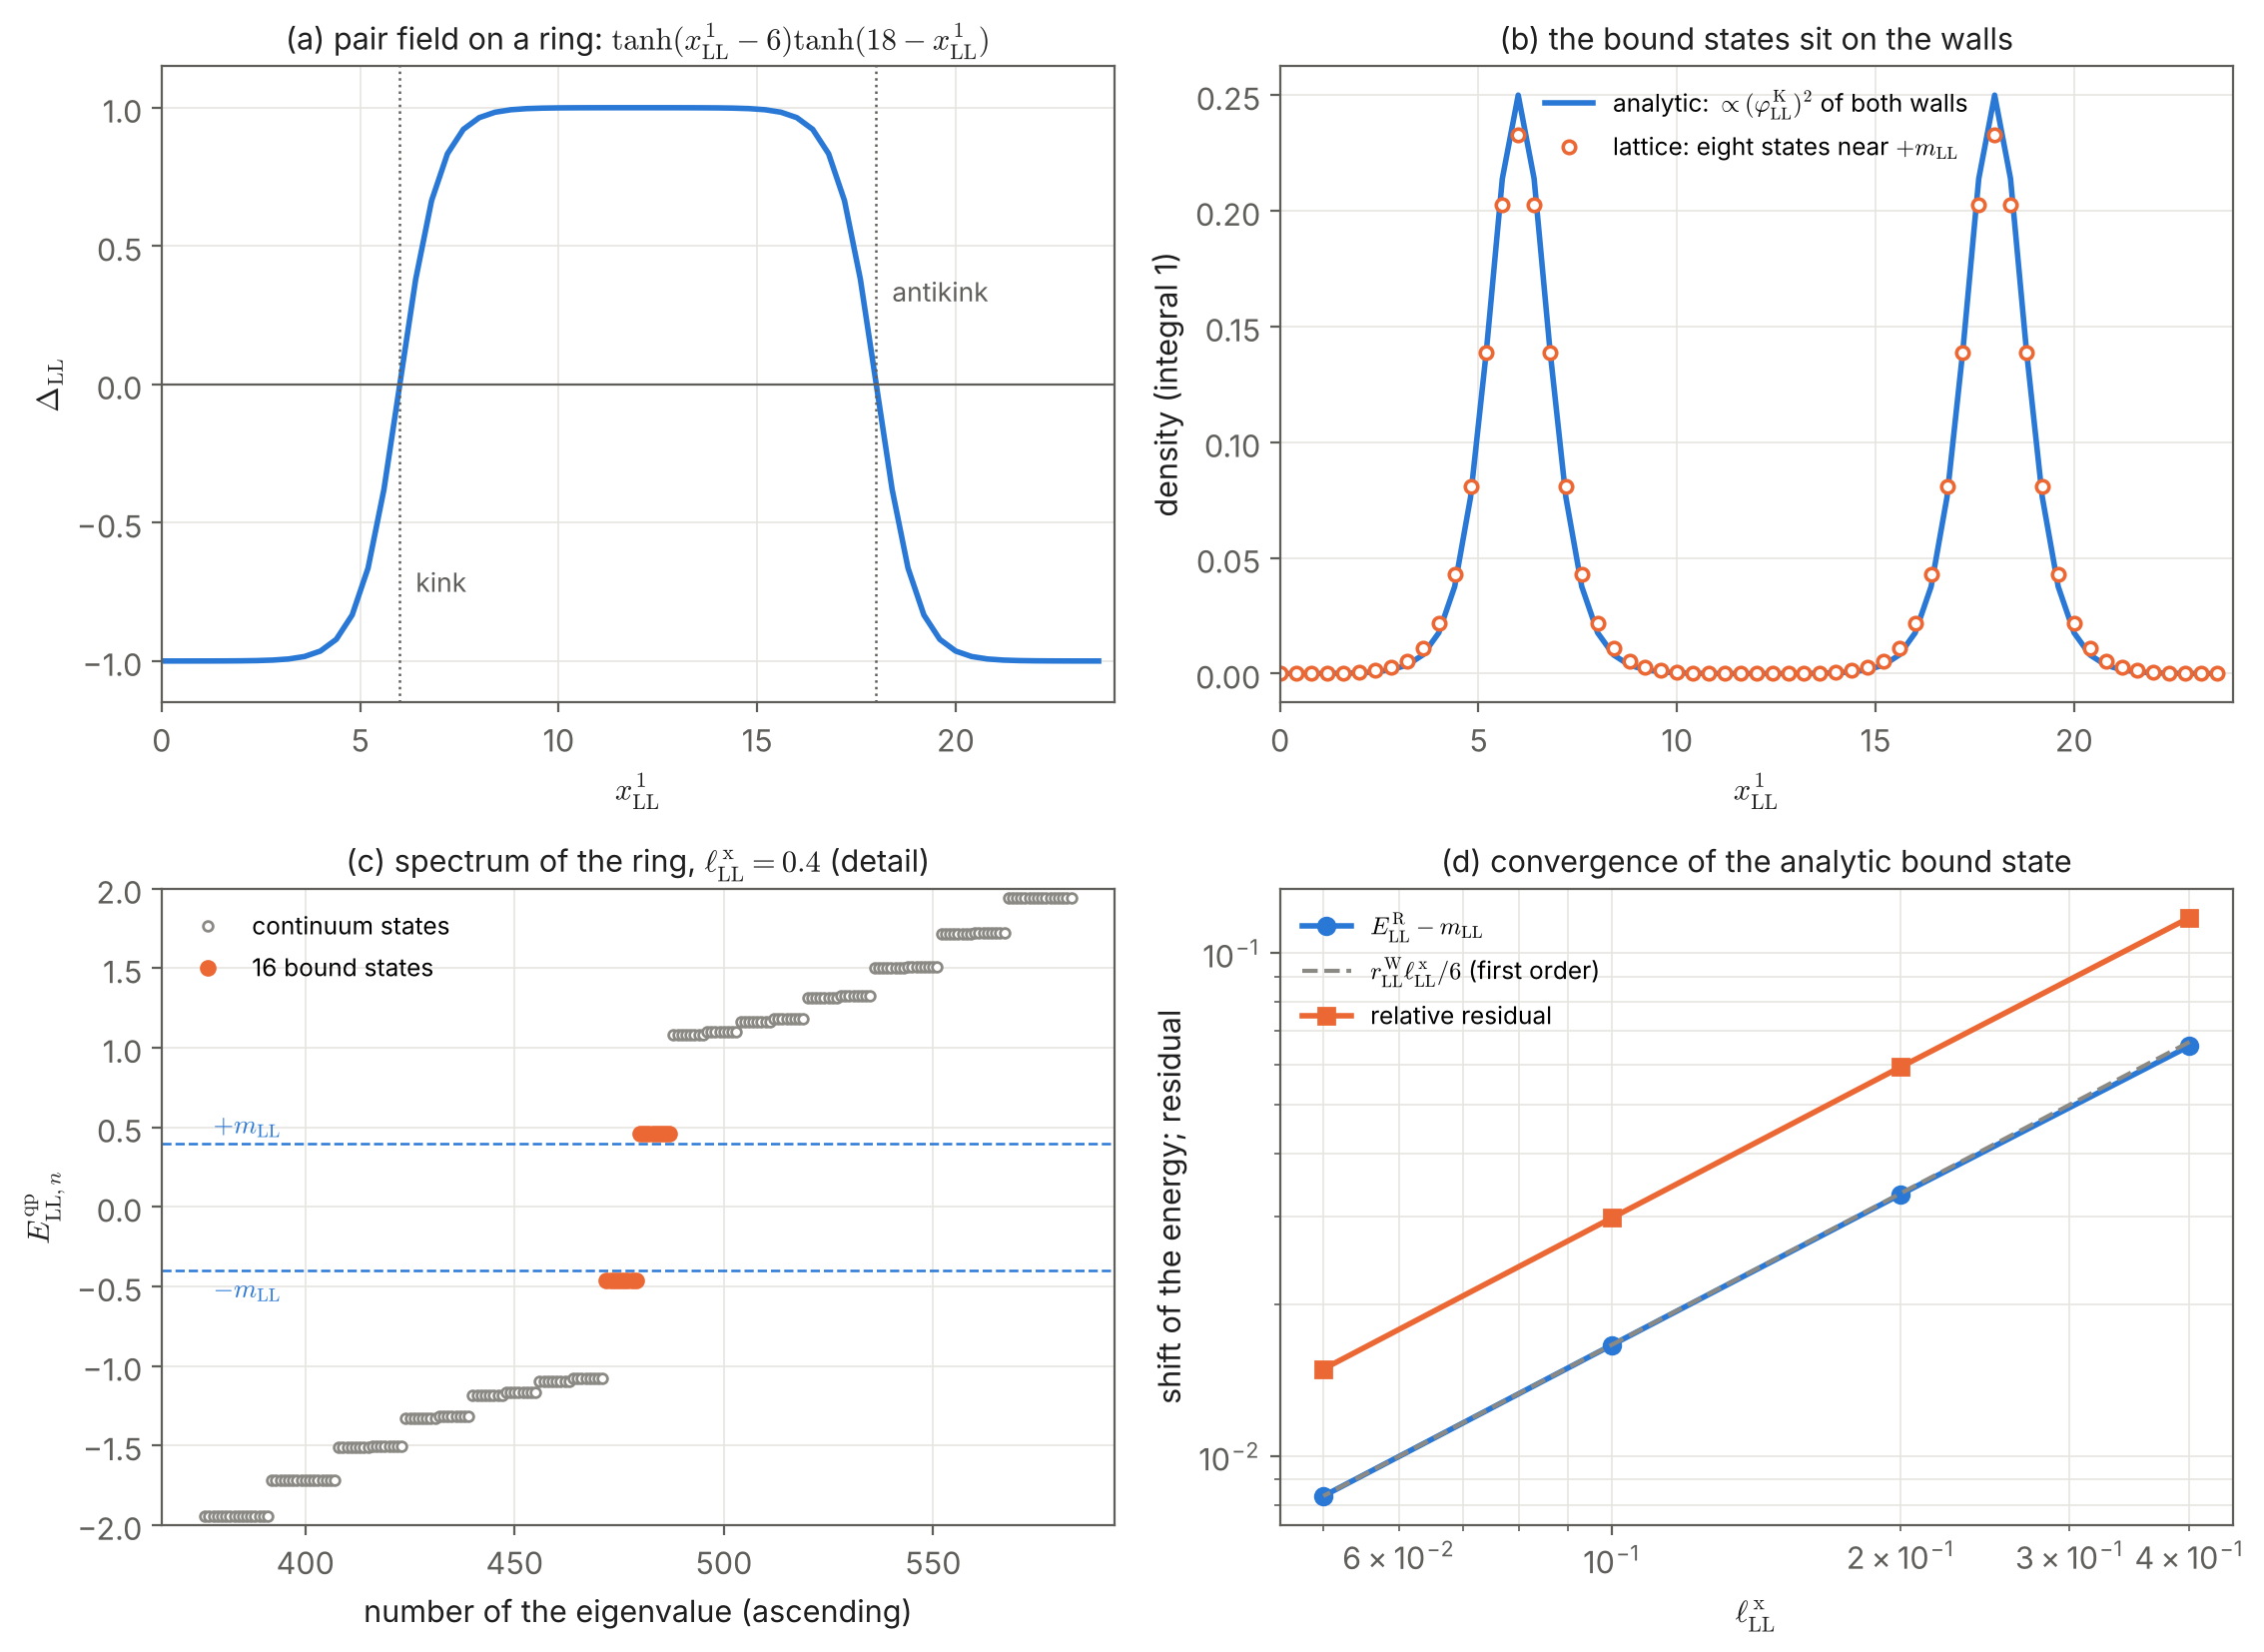
\includegraphics[width=1\textwidth,height=\textheight]{figures/fig_t2_case_C.png}

\textbf{Figure 5.} Case C, a domain wall of the pair field, on a ring of
length 24 with a kink at \(x^1_{\rm LL}=6\) and an antikink at
\(x^1_{\rm LL}=18\) (\(m_{\rm LL}=0.4\), \(\mu_{\rm LL}=0\),
\(r^{\rm W}_{\rm LL}=1\)). (a) The pair field. (b) The summed density of
the eight eigenvectors of the lattice operator with energies near
\(+m_{\rm LL}\) (\(\ell^{\rm x}_{\rm LL}=0.4\), circles) and the
analytic density, proportional to \((\varphi^{\rm K}_{\rm LL})^2\) of
the two walls (line), both normalized to the integral 1. (c) The
spectrum of the ring near zero energy: the 16 bound states (orange) lie
inside the gap of the continuum states (grey), near \(\pm m_{\rm LL}\)
(dashed). (d) The convergence of the analytic bound state: the shift
\(E^{\rm R}_{\rm LL}-m_{\rm LL}\) of its Rayleigh quotient (blue)
follows \(r^{\rm W}_{\rm LL}\ell^{\rm x}_{\rm LL}/6\) (grey, dashed),
and its residual (orange) falls in proportion to
\(\ell^{\rm x}_{\rm LL}\). Data:
\texttt{test2/data/t2\_C\_kink\_profile.csv},
\texttt{t2\_C\_kink\_spectrum.csv},
\texttt{t2\_C\_kink\_convergence.csv}.

\hypertarget{case-d-landau-levels-in-constant-magnetic-fields}{%
\subsection{3.5 Case D: Landau levels in constant magnetic
fields}\label{case-d-landau-levels-in-constant-magnetic-fields}}

\textbf{The fields.} No pair field, \(\mu_{\rm LL}=0\), and constant
magnetic fields along \(x^3_{\rm LL}\) of the phase group and of the
third isospin direction, \(\mathsf F^{\rm F}_{{\rm LL},12}\) and
\(\mathsf F^3_{{\rm LL},12}\), in the Landau gauge
\(A^{\rm F}_{{\rm LL},2}=\mathsf F^{\rm F}_{{\rm LL},12}x^1_{\rm LL}\),
\(A^3_{{\rm LL},2}=\mathsf F^3_{{\rm LL},12}x^1_{\rm LL}\) (all other
potentials zero; then \(\partial_1A^{\rm F}_{{\rm LL},2}\) and
\(\partial_1A^3_{{\rm LL},2}\) are the fields, and the commutator term
of \(\mathsf F^3_{{\rm LL},12}\) vanishes because
\(A^\iota_{{\rm LL},1}=0\)). On the isospin-up component the potential
is \(\mathsf A^\uparrow_{{\rm LL},2}=B^\uparrow_{\rm LL}x^1_{\rm LL}\),
on the isospin-down component \(B^\downarrow_{\rm LL}x^1_{\rm LL}\),
with

\[B^\uparrow_{\rm LL}=g^{\rm F}_{\rm LL}\mathsf F^{\rm F}_{{\rm LL},12}+\tfrac12g^{\rm v}_{\rm LL}\mathsf F^3_{{\rm LL},12},\qquad B^\downarrow_{\rm LL}=g^{\rm F}_{\rm LL}\mathsf F^{\rm F}_{{\rm LL},12}-\tfrac12g^{\rm v}_{\rm LL}\mathsf F^3_{{\rm LL},12}:\tag{3.30}\]

the two isospin components feel different magnetic fields.

\textbf{The solution.} By (3.4), on the isospin-up component and on
\(\exp(i(q^2_{\rm LL}x^2_{\rm LL}+q^3_{\rm LL}x^3_{\rm LL}))\) times a
function of \(x^1_{\rm LL}\),

\[(h^\nabla_{\rm LL})^2=m_{\rm LL}^2+(q^3_{\rm LL})^2+\Big(-\frac{d^2}{d(x^1_{\rm LL})^2}+(B^\uparrow_{\rm LL})^2\big(x^1_{\rm LL}-q^2_{\rm LL}/B^\uparrow_{\rm LL}\big)^2\Big)-2B^\uparrow_{\rm LL}\,i\,\mathsf s_{\rm LL}(J^3_{\rm LL}).\tag{3.31}\]

The bracket is a harmonic oscillator centred at
\(x^1_{\rm LL}=q^2_{\rm LL}/B^\uparrow_{\rm LL}\), with the eigenvalues
\(\lvert B^\uparrow_{\rm LL}\rvert\) times \(1,3,5,\dots\); the spin
\(i\,\mathsf s_{\rm LL}(J^3_{\rm LL})\) has the eigenvalues
\(\pm\tfrac12\) and commutes with the bracket. The sum of the oscillator
energy and the spin energy \(\mp B^\uparrow_{\rm LL}\) is
\(2n^{\rm L}_{\rm LL}\lvert B^\uparrow_{\rm LL}\rvert\), where the level
\(n^{\rm L}_{\rm LL}=0\) arises only from the lowest oscillator state
with the spin parallel to \(B^\uparrow_{\rm LL}\), and each level
\(n^{\rm L}_{\rm LL}\ge1\) from two combinations (the oscillator state
number \(n^{\rm L}_{\rm LL}\) with the parallel spin and
\(n^{\rm L}_{\rm LL}-1\) with the antiparallel spin). So

\[E^{\rm qp}_{{\rm LL},n}=\pm\big(m_{\rm LL}^2+(q^3_{\rm LL})^2+2n^{\rm L}_{\rm LL}\lvert B^\uparrow_{\rm LL}\rvert\big)^{1/2},\qquad n^{\rm L}_{\rm LL}=0,1,2,\dots,\tag{3.32}\]

for each \(q^2_{\rm LL}\) (the position of the centre: the levels are
degenerate, with \(\lvert B^\uparrow_{\rm LL}\rvert/(2\pi)\) states per
unit area of the plane \(x^1_{\rm LL}\), \(x^2_{\rm LL}\)), and the same
with \(B^\downarrow_{\rm LL}\) for isospin down. At \(q^3_{\rm LL}=0\)
the level \(n^{\rm L}_{\rm LL}=0\) has the energies \(+m_{\rm LL}\) and
\(-m_{\rm LL}\) once each, and every level \(n^{\rm L}_{\rm LL}\ge1\)
has each of its two energies twice. The level \(n^{\rm L}_{\rm LL}=0\)
does not depend on the field: the spin energy cancels the zero-point
energy of the oscillator exactly, because the gyromagnetic factor is 2
(3.5). For slow charges (3.32) gives
\(m_{\rm LL}+(q^3_{\rm LL})^2/(2m_{\rm LL})+n^{\rm L}_{\rm LL}\lvert B^\uparrow_{\rm LL}\rvert/m_{\rm LL}\),
equally spaced levels with the cyclotron frequency
\(\lvert B^\uparrow_{\rm LL}\rvert/m_{\rm LL}\). Check AS-10
diagonalizes \(h^\nabla_{\rm LL}\) at \(q^2_{\rm LL}=q^3_{\rm LL}=0\) in
a basis of 120 oscillator states for both isospin components
(\(\mathsf F^{\rm F}_{{\rm LL},12}=1.2\),
\(\mathsf F^3_{{\rm LL},12}=1.0\), so \(B^\uparrow_{\rm LL}=0.89\) and
\(B^\downarrow_{\rm LL}=0.19\)) and finds (3.32) with these
multiplicities to \(10^{-14}\) for \(n^{\rm L}_{\rm LL}=0\) to 10. (The
exact eigenstates of the level \(n^{\rm L}_{\rm LL}\) contain the
oscillator states \(n^{\rm L}_{\rm LL}-1\) and \(n^{\rm L}_{\rm LL}\)
only, so the truncated basis represents them exactly; the truncation
creates spurious states on the highest oscillator states, which the
check recognizes by their weight there and discards.)

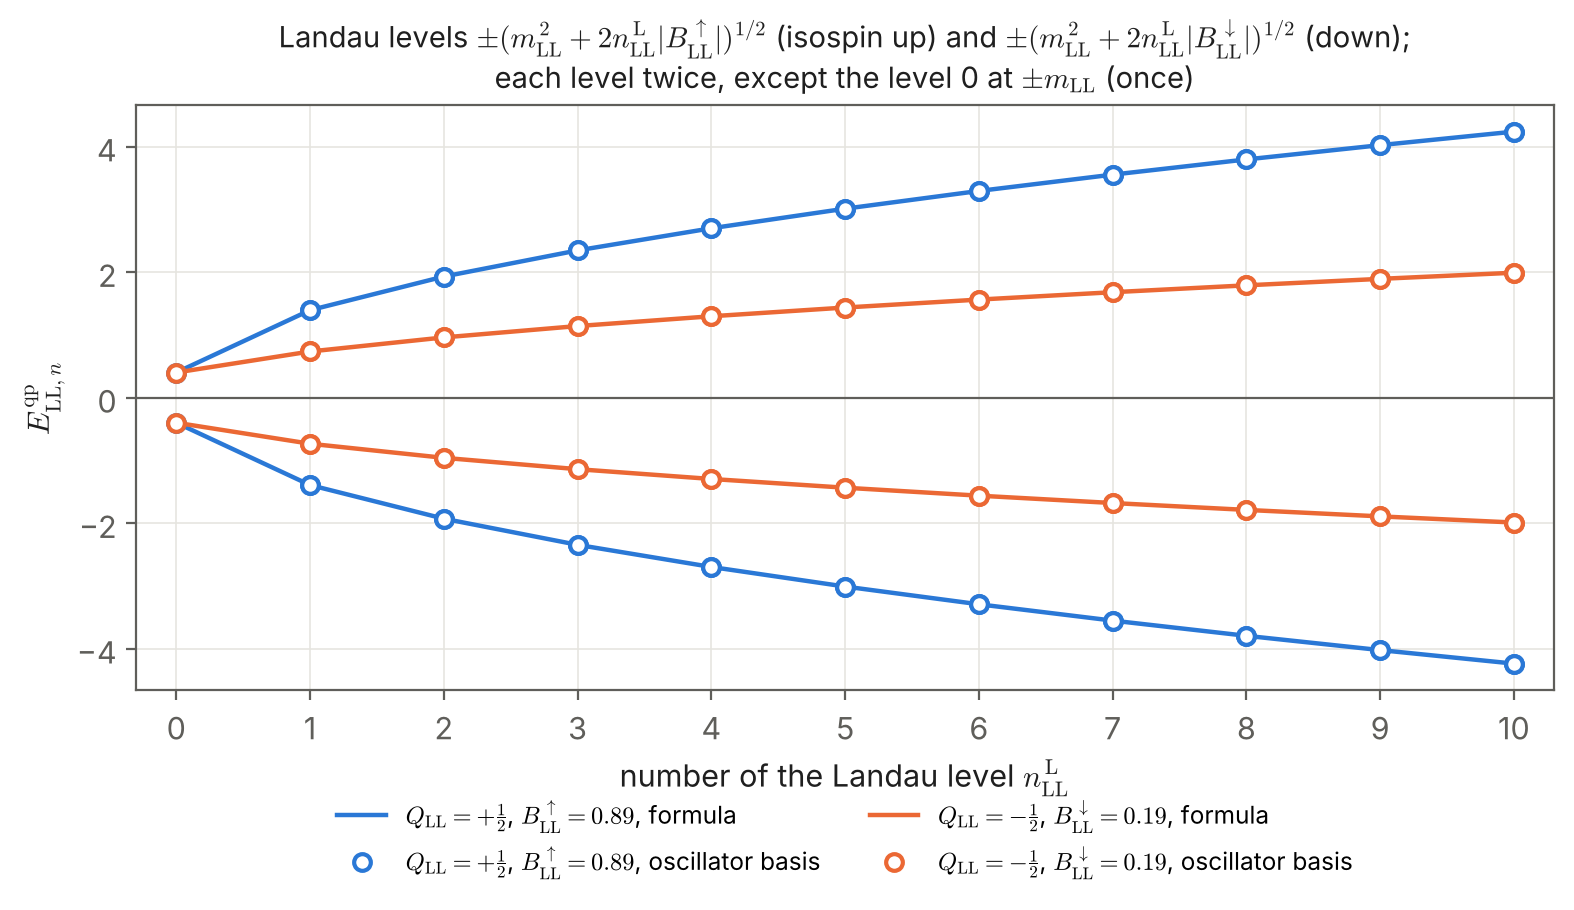
\includegraphics[width=0.8\textwidth,height=\textheight]{figures/fig_t2_case_D.png}

\textbf{Figure 6.} Case D, the Landau levels (3.32) at
\(q^3_{\rm LL}=0\) for isospin up (\(B^\uparrow_{\rm LL}=0.89\), blue)
and down (\(B^\downarrow_{\rm LL}=0.19\), orange), \(m_{\rm LL}=0.4\):
the formula (lines) and the eigenvalues of the oscillator-basis
diagonalization (circles; each level \(n^{\rm L}_{\rm LL}\ge1\) is a
pair of coinciding eigenvalues). Data:
\texttt{test2/data/t2\_D\_landau.csv}.

\hypertarget{discussion-1}{%
\subsection{3.6 Discussion}\label{discussion-1}}

\begin{itemize}
\tightlist
\item
  \textbf{What each case tests.} Case A tests the covariant derivative:
  the space potentials enter as a shift of the momentum, the time
  potential as a shift of the energy, the isospin potential as a
  rotation, all exactly as minimal coupling requires. Case B tests the
  pair field and the self-consistency: the Bogoliubov spectrum, the
  particle-hole conversion, the gap equation, and an exact fixed point
  of the lattice mean-field equations. Case C tests a non-uniform pair
  field and the lattice discretization: the bound states are fixed by
  the topology of the wall, and the lattice reproduces them up to the
  Wilson shift \(r^{\rm W}_{\rm LL}\ell^{\rm x}_{\rm LL}/6\). Case D
  tests the field strengths: the magnetic moment of the spinor charges
  has the gyromagnetic factor 2 for both the phase and the isospin
  charges.
\item
  \textbf{What is gauge invariant.} The spectra are (including their
  shifts by holonomies on a ring), as are the field strengths and
  \(\lvert d^\iota_{\rm LL}\rvert\). The isospin direction of a single
  mode and the phase of the pair field are not: the precession (3.8)
  disappears in another gauge.
\item
  \textbf{Test problems for the solvers of items {[}3{]} and {[}5{]}.}
  The time-dependent solutions (3.8) and (3.15) test the RK4 time
  stepping with gauge potentials and with a pair field; (3.21) is a
  fixed point of the self-consistent iteration; the bound states (3.24),
  (3.29) test non-uniform pair fields; the fermion number (3.3) is
  conserved in every self-consistent evolution.
\item
  \textbf{Limits.} The cases are uniform or depend on one coordinate.
  General fields, several walls at short distance, time-dependent gauge
  fields and the self-consistent dynamics of the pair field need the
  numerical solution of items {[}3{]} to {[}6{]}.
\end{itemize}

\hypertarget{item-3-a-python-program-that-solves-the-field-equations}{%
\section{4. Item {[}3{]}: a Python program that solves the field
equations}\label{item-3-a-python-program-that-solves-the-field-equations}}

\hypertarget{the-answer-in-brief-2}{%
\subsection{4.0 The answer in brief}\label{the-answer-in-brief-2}}

\begin{enumerate}
\def\labelenumi{\arabic{enumi}.}
\tightlist
\item
  \textbf{The program.} \texttt{test2/python/t2\_solve.py} (Python 3
  with NumPy and SciPy, about 1750 commented lines) solves the
  mean-field field equations (2.31), (2.32) of the self-interacting
  spinor field on the lattice of Section 2.11, with the gauge-covariant
  central difference (2.35) (the link matrices (2.34)), the Wilson term,
  constant or site-dependent gauge potentials, constant magnetic fields,
  a pulse of a gauge field in time, and a prescribed or self-consistent
  pair field. Its lattice operator is the operator (2.36) of Section
  2.11, built as a sparse matrix; a self-test compares it with an
  independent site-by-site implementation.
\item
  \textbf{Guidance and input.} Started without arguments, the program
  explains how to define the initial and the boundary conditions, offers
  ready examples, and asks for the name of an input file. The input file
  is a plain text file of lines \texttt{key\ =\ value}; every key is
  listed in Section 4.2 (the table is written by the program itself).
  The program checks every value and stops with a precise message if a
  key is unknown, misspelt, given twice, or out of range.
\item
  \textbf{Four tasks.} \texttt{evolve} (the time evolution of one mode
  in prescribed fields, by RK4), \texttt{spectrum} (all eigenvalues and
  the bound states), \texttt{ground\_state} (the self-consistent pair
  field, by Anderson-accelerated iteration) and \texttt{quench} (the
  self-consistent evolution of all modes after a change of the coupling,
  by the implicit midpoint rule, which conserves the orthonormality of
  the modes and the fermion number exactly).
\item
  \textbf{Seven examples} (folder \texttt{test2/examples}), each with a
  known answer: a free wave packet (it moves with the group velocity of
  (2.37)); a packet in a magnetic field (a bounded orbit); a particle
  hitting a superfluid region (Andreev reflection into a hole); the
  bound states of a kink and an antikink (Section 3.4); the
  self-consistent uniform superfluid (the gap equation (3.21)); a
  self-consistent kink; and a quench of the coupling (the amplitude mode
  of the pair field, the analogue of the Higgs boson). All checks of the
  program (4 in the self-test, 3 to 5 per example) and all 10
  independent checks EX-1 to EX-7 of the program
  \texttt{t2\_examples\_check.py} pass. The numerical results are
  plotted by the program of item {[}4{]} (Section 5).
\end{enumerate}

\hypertarget{how-to-use-the-program}{%
\subsection{4.1 How to use the program}\label{how-to-use-the-program}}

\textbf{Requirements.} Python 3.8 or later with NumPy and SciPy
(\texttt{python3\ -m\ pip\ install\ numpy\ scipy}). The program runs
from any folder; the commands below are given from the folder
Revision\_SuperLoop of the repository.

\textbf{Step by step.}

\begin{verbatim}
# 1. read the guide: what is solved, how the initial and boundary conditions are defined, and every key
python3 test2/python/t2_solve.py --guide
# 2. list the examples, and write one of them as a commented input file to start from
python3 test2/python/t2_solve.py --examples
python3 test2/python/t2_solve.py --example andreev my_problem.t2in
# 3. edit my_problem.t2in with any text editor, then solve it
python3 test2/python/t2_solve.py my_problem.t2in
# 4. or start the program without arguments: it prints a short guide and asks for the name of the input file
python3 test2/python/t2_solve.py
# 5. optional: check the lattice operator of the program (self-test)
python3 test2/python/t2_solve.py --selftest
\end{verbatim}

In the dialogue of step 4 the program answers \texttt{?} with the
complete guide, \texttt{examples} with the list of examples,
\texttt{example\ NAME} by writing that example as \texttt{NAME.t2in},
and a file name by solving that file; \texttt{q} ends it. The output
files are named after the input file (\texttt{my\_problem\_summary.txt}
and so on) and are written into the folder of the input file, unless the
key \texttt{output} or the option \texttt{-\/-out\ BASE} (for example
\texttt{-\/-out\ results/run1}) names another base.

\textbf{How to define the boundary conditions.} The key \texttt{sites}
gives the numbers of sites \(n^{\rm x}_{\rm LL}\),
\(n^{\rm y}_{\rm LL}\), \(n^{\rm z}_{\rm LL}\) along \(x^1_{\rm LL}\),
\(x^2_{\rm LL}\), \(x^3_{\rm LL}\), and \texttt{spacing} the spacing
\(\ell^{\rm x}_{\rm LL}\); the coordinates \(x^j_{\rm LL}\) of the sites
are the multiples of \(\ell^{\rm x}_{\rm LL}\) from 0 to
\(\ell^{\rm x}_{\rm LL}\) times the number of sites of that direction
minus 1. A direction with one site is absent: the fields do not depend
on that coordinate (one- and two-dimensional problems). The key
\texttt{boundary} gives three words, one per direction:
\texttt{periodic} (the last site is the neighbour of the first; the
lattice is a ring or a torus, and a constant potential acts through its
holonomy) or \texttt{wall} (the field vanishes beyond the last site: a
hard wall, the Dirichlet condition of Section 2.11).

\textbf{How to define the initial conditions.} For the task
\texttt{evolve} the key \texttt{initial} chooses the initial mode:
\texttt{packet} (a Gaussian wave packet, defined by
\texttt{packet\_center}, \texttt{packet\_width},
\texttt{packet\_momentum}, \texttt{packet\_branch},
\texttt{packet\_spin}, \texttt{packet\_isospin} and
\texttt{packet\_part}; Section 4.3), \texttt{eigenmode} (an eigenvector
of the lattice operator, chosen by its number in the ascending list) or
\texttt{file} (all
\(16\,n^{\rm x}_{\rm LL}n^{\rm y}_{\rm LL}n^{\rm z}_{\rm LL}\) complex
components from a file, one line \texttt{re\ im} each, in the order of
the components of Section 2.11). For \texttt{ground\_state} and
\texttt{quench} the initial condition is the initial guess of the pair
field, given by the key \texttt{pair}; the quench starts from the
converged ground state.

\textbf{How to define the fields.} Constant potentials with
\texttt{potential\_0} to \texttt{potential\_3} (each four numbers
\(A^1_{{\rm LL},p}\), \(A^2_{{\rm LL},p}\), \(A^3_{{\rm LL},p}\),
\(A^{\rm F}_{{\rm LL},p}\)); potentials that depend on the site from a
file (\texttt{gauge\_file}: one line per site with 16 numbers, the four
potentials of \(p=0,1,2,3\) in this order); constant magnetic fields
along \(x^3_{\rm LL}\) with \texttt{magnetic}
(\(\mathsf F^{\rm F}_{{\rm LL},12}\) and \(\mathsf F^3_{{\rm LL},12}\),
in the Landau gauge of Section 3.5, centred on the lattice); and a
uniform pulse in time of the four potentials of one index \(p\)
(\texttt{pulse\_direction}, \texttt{pulse\_potential},
\texttt{pulse\_time}). All contributions are added, and the links (2.34)
of a site use the potentials at that site. The pair field is chosen by
\texttt{pair}: \texttt{none}, \texttt{uniform}, \texttt{kink},
\texttt{kink\_antikink}, \texttt{step}, \texttt{random} or
\texttt{file}, with its isospin direction, amplitude, phase, width and
the positions of its walls (Section 4.2).

\hypertarget{the-input-file}{%
\subsection{4.2 The input file}\label{the-input-file}}

The file is plain text. Each line holds one entry
\texttt{key\ =\ value}; the character \texttt{\#} starts a comment;
empty lines are ignored; the order of the keys is free. The first entry
must be \texttt{format\ =\ t2in\ 1}. A key that the program does not
know is an error (with a suggestion of the key that was probably meant),
so that a misspelt key cannot be ignored silently. A key that is not
given takes its default. The table lists every key; it is written by the
program from the very table that it uses to read the file
(\texttt{python3\ test2/python/t2\_solve.py\ -\/-keys-md\ FILE}), so
that it cannot differ from the program.

\begin{longtable}[]{@{}
  >{\raggedright\arraybackslash}p{(\columnwidth - 6\tabcolsep) * \real{0.2131}}
  >{\raggedright\arraybackslash}p{(\columnwidth - 6\tabcolsep) * \real{0.1311}}
  >{\raggedright\arraybackslash}p{(\columnwidth - 6\tabcolsep) * \real{0.1311}}
  >{\raggedright\arraybackslash}p{(\columnwidth - 6\tabcolsep) * \real{0.5246}}@{}}
\toprule\noalign{}
\begin{minipage}[b]{\linewidth}\raggedright
key
\end{minipage} & \begin{minipage}[b]{\linewidth}\raggedright
value
\end{minipage} & \begin{minipage}[b]{\linewidth}\raggedright
default
\end{minipage} & \begin{minipage}[b]{\linewidth}\raggedright
meaning
\end{minipage} \\
\midrule\noalign{}
\endhead
\bottomrule\noalign{}
\endlastfoot
\texttt{format} & text & required & the format of the file; must be
`t2in 1' \\
\texttt{title} & text & (see text) & a free title of the problem \\
\texttt{task} & one of: evolve, spectrum, ground\_state, quench &
required & what to solve (see the guide) \\
\texttt{output} & text & (see text) & the base name of the output files,
relative to the folder of the input file (default: the name of the input
file without its extension) \\
\texttt{sites} & three integers & required & the numbers of lattice
sites n\_x n\_y n\_z along x\^{}1, x\^{}2, x\^{}3; 1 means that the
fields do not depend on that coordinate \\
\texttt{spacing} & positive number & required & the lattice spacing dx
(the same in all directions) \\
\texttt{boundary} & three words, each: periodic, wall & periodic
periodic periodic & the boundary condition of each direction: periodic
(a ring) or wall (the field vanishes beyond the last site: Dirichlet) \\
\texttt{wilson} & number \textgreater= 0 & 1.0 & the coefficient r\_W of
the Wilson term (removes the doublers; 1 is standard) \\
\texttt{mass} & number & 0.4 & the mass m of the spinor charges \\
\texttt{mu} & number & 0.0 & the chemical potential mu \\
\texttt{g\_v} & number & 0.7 & the isospin coupling g\_v \\
\texttt{g\_F} & number & 0.45 & the coupling g\_F of the phase group \\
\texttt{potential\_0} & four numbers & 0 0 0 0 & the constant potentials
A\^{}1\_0 A\^{}2\_0 A\^{}3\_0 A\^{}F\_0 (time direction) \\
\texttt{potential\_1} & four numbers & 0 0 0 0 & the constant potentials
A\^{}1\_1 A\^{}2\_1 A\^{}3\_1 A\^{}F\_1 (direction x\^{}1) \\
\texttt{potential\_2} & four numbers & 0 0 0 0 & the constant potentials
A\^{}1\_2 A\^{}2\_2 A\^{}3\_2 A\^{}F\_2 (direction x\^{}2) \\
\texttt{potential\_3} & four numbers & 0 0 0 0 & the constant potentials
A\^{}1\_3 A\^{}2\_3 A\^{}3\_3 A\^{}F\_3 (direction x\^{}3) \\
\texttt{magnetic} & two numbers & 0 0 & constant magnetic fields along
x\^{}3: F\^{}F\_12 (phase group) and F\^{}3\_12 (third isospin
direction), in the Landau gauge A\_2 = F (x\^{}1 - centre); needs n\_x
\textgreater{} 1, n\_y \textgreater{} 1 and a wall in direction 1 \\
\texttt{gauge\_file} & text & (see text) & a file with potentials that
depend on the site (added to the constant ones): one line per site, in
the order of the sites, with 16 numbers A\^{}1\_p A\^{}2\_p A\^{}3\_p
A\^{}F\_p for p = 0, 1, 2, 3 \\
\texttt{pulse\_direction} & 0, 1, 2 or 3 & 1 & the index p (0, 1, 2 or
3) of the potential A\_p that carries the pulse \\
\texttt{pulse\_potential} & four numbers & 0 0 0 0 & the amplitudes
A\^{}1 A\^{}2 A\^{}3 A\^{}F of a uniform pulse of the potential A\_p
(all zero: no pulse) \\
\texttt{pulse\_time} & three numbers & 5 1 0 & the centre t\_c, the
duration t\_w and the angular frequency w\_p of the pulse: A\_p(x\^{}0)
= amplitudes exp(-(x\^{}0 - t\_c)\^{}2/(2 t\_w\^{}2)) cos(w\_p (x\^{}0 -
t\_c)) \\
\texttt{pair} & one of: none, uniform, kink, kink\_antikink, step,
random, file & none & the profile of the pair field d\^{}iota:
prescribed (evolve, spectrum) or the initial guess (ground\_state,
quench) \\
\texttt{pair\_direction} & 1, 2 or 3 & 3 & the isospin direction iota of
the pair field (1, 2 or 3) \\
\texttt{pair\_amplitude} & number & 0.0 & the gap Delta (uniform, step)
or Delta\_inf (kinks) \\
\texttt{pair\_phase} & number & 0.0 & the phase of the pair field, in
radians \\
\texttt{pair\_width} & positive number & 1.0 & the width ell\_K of a
kink or of a step \\
\texttt{pair\_position} & numbers & (see text) & the positions along
x\^{}1 of the walls (kink: one value, default the centre;
kink\_antikink: two values, default 1/4 and 3/4 of the length; step: one
value, default the centre) \\
\texttt{pair\_seed} & integer & 1 & the seed of the random pair field
(pair = random) \\
\texttt{pair\_file} & text & (see text) & a file with the pair field
(pair = file): one line per site, in the order of the sites, with d1\_re
d1\_im d2\_re d2\_im d3\_re d3\_im \\
\texttt{time\_step} & positive number & required for evolve, quench &
the time step dt (evolve, quench) \\
\texttt{steps} & positive integer & required for evolve, quench & the
number of time steps (evolve, quench) \\
\texttt{output\_every} & positive integer & 0 & write the fields on the
sites every this many steps (0: about 50 outputs); the time series is
written at every step \\
\texttt{initial} & one of: packet, eigenmode, file & packet & the
initial mode of the task evolve \\
\texttt{packet\_center} & three numbers & (see text) & the centre of the
Gaussian packet (x\^{}1 x\^{}2 x\^{}3; default the centre of the
lattice) \\
\texttt{packet\_width} & positive number & 2.0 & the width of the packet
(standard deviation of the density) \\
\texttt{packet\_momentum} & three numbers & 0 0 0 & the momentum q of
the packet \\
\texttt{packet\_branch} & one of: positive, negative & positive & the
sign of the energy +-eps\_lat(q) of the free lattice operator (without
mu) of the packet \\
\texttt{packet\_spin} & one of: up, down & up & the spin along x\^{}3 of
the reference spinor \\
\texttt{packet\_isospin} & one of: up, down & up & the isospin
component \\
\texttt{packet\_part} & one of: particle, hole & particle & particle
part or hole part of the mode \\
\texttt{eigenmode\_index} & integer & 0 & the number (ascending, from 0)
of the eigenvector used as initial mode (initial = eigenmode) \\
\texttt{initial\_file} & text & (see text) & a file with the initial
mode (initial = file): 16 x (number of sites) lines `re im' in the order
of the components \\
\texttt{spectrum\_window} & two numbers & -1 1 & the energy window of
the eigenvectors whose densities are written (spectrum) \\
\texttt{spectrum\_max\_states} & positive integer & 32 & at most this
many eigenvectors of the window are written (spectrum), summed over each
group of degenerate eigenvalues \\
\texttt{coupling} & positive number & required for ground\_state, quench
& the coupling G of the self-consistency condition (ground\_state,
quench) \\
\texttt{pair\_constraint} & one of: none, line & none & line: the
self-consistent iteration keeps the pair field a real multiple of exp(i
pair\_phase) along pair\_direction (for walls of the pair field, which
are unstable without it) \\
\texttt{mixing} & number in (0, 1{]} & 0.5 & the damping factor beta of
the Anderson iteration (ground\_state, quench) \\
\texttt{tolerance} & positive number & 1e-10 & the iteration stops when
the largest change of d\^{}iota is below this \\
\texttt{max\_iterations} & positive integer & 400 & the largest number
of iterations \\
\texttt{quench\_coupling} & positive number & required for quench & the
coupling after x\^{}0 = 0 (quench) \\
\end{longtable}

In the table, \texttt{dx} is \(\ell^{\rm x}_{\rm LL}\), \texttt{dt} is
\(\ell^{\rm t}_{\rm LL}\), \texttt{r\_W} is \(r^{\rm W}_{\rm LL}\),
\texttt{m} is \(m_{\rm LL}\), \texttt{mu} is \(\mu_{\rm LL}\),
\texttt{g\_v} and \texttt{g\_F} are \(g^{\rm v}_{\rm LL}\) and
\(g^{\rm F}_{\rm LL}\), \texttt{G} is \(G_{\rm LL}\), \texttt{Delta} and
\texttt{Delta\_inf} are \(\Delta_{\rm LL}\) and
\(\Delta^\infty_{\rm LL}\), \texttt{ell\_K} is
\(\ell^{\rm K}_{\rm LL}\), \texttt{d\^{}iota} is \(d^\iota_{\rm LL}\),
\texttt{A\^{}1\_p} to \texttt{A\^{}F\_p} are \(A^1_{{\rm LL},p}\) to
\(A^{\rm F}_{{\rm LL},p}\), \texttt{F\^{}F\_12} and \texttt{F\^{}3\_12}
are \(\mathsf F^{\rm F}_{{\rm LL},12}\) and
\(\mathsf F^3_{{\rm LL},12}\), \texttt{eps\_lat(q)} is
\(\varepsilon^{\rm lat}_{\rm LL}(\vec q_{\rm LL})\), \texttt{Hbound} is
\(B^{\rm H}_{\rm LL}\), and \texttt{x\^{}0}, \texttt{x\^{}1} are
\(x^0_{\rm LL}\), \(x^1_{\rm LL}\). The pulse adds to the potential of
the direction \texttt{pulse\_direction} the four amplitudes of
\texttt{pulse\_potential} times the factor
\texttt{exp(-(x\^{}0\ -\ t\_c)\^{}2/(2\ t\_w\^{}2))\ cos(w\_p\ (x\^{}0\ -\ t\_c))},
where \texttt{t\_c}, \texttt{t\_w}, \texttt{w\_p} are the three numbers
of \texttt{pulse\_time} (the centre, the duration and the angular
frequency of the pulse), uniformly on all sites.

\hypertarget{what-the-program-computes}{%
\subsection{4.3 What the program
computes}\label{what-the-program-computes}}

\textbf{The lattice operator.} The program builds
\(\mathcal H^{\rm lat}_{\rm LL}\) of (2.36) as a sparse matrix from
\(8\times8\) blocks: on each site the block
\((m_{\rm LL}+r^{\rm W}_{\rm LL}n^{\rm act}_{\rm LL}/\ell^{\rm x}_{\rm LL})\beta_{\rm LL}\otimes\sigma^{\rm LL}_0-\mathsf 1_4\otimes(\mathsf A_{{\rm LL},0}+\mu_{\rm LL}\sigma^{\rm LL}_0)\)
(the mass, the diagonal part of the Wilson term, the potential and the
chemical potential), where \(n^{\rm act}_{\rm LL}\) is the number of
active directions (the directions with more than one site); for each
active direction \(j\) the block
\((-i\alpha^j_{\rm LL}-r^{\rm W}_{\rm LL}\beta_{\rm LL})/(2\ell^{\rm x}_{\rm LL})\otimes\mathsf U^{\rm link}_{{\rm LL},j}(\vec s_{\rm LL})\)
from the site \(\vec s_{\rm LL}\) to its forward neighbour and the block
\((i\alpha^j_{\rm LL}-r^{\rm W}_{\rm LL}\beta_{\rm LL})/(2\ell^{\rm x}_{\rm LL})\otimes\mathsf U^{\rm link}_{{\rm LL},j}(\vec s_{\rm LL}-\vec\delta^j_{\rm LL})^\dagger\)
to its backward neighbour (a missing neighbour at a wall gives no
block). These blocks act on the particle components; the hole components
receive the complex conjugate blocks with the opposite sign, and the
pair field the blocks
\(\mathsf P_{\rm LL}=\sum_\iota d^\iota_{\rm LL}(\mathsf K^\iota_{\rm LL})^\dagger\)
and \(\mathsf P^\dagger_{\rm LL}\) on each site. This is (2.36) term by
term. The self-test applies the matrix to five random vectors on a
lattice of \(3\times4\times2\) sites with random links, potentials and
pair field, periodic and wall directions, and compares with a direct
site-by-site evaluation of (2.36): the largest difference is
\(7\times10^{-15}\). It also checks that the matrix is Hermitian, that
the closed form (2.34) of the links equals the exponential of the
generator computed by the general matrix exponential of SciPy (to
\(2\times10^{-16}\)), and that the 256 eigenvalues of a ring of 16 sites
in constant potentials are the energies of case A, check AS-1 (to
\(1.4\times10^{-14}\)).

\textbf{The normalization in fewer than three dimensions.} A problem
with \(n^{\rm act}_{\rm LL}\) active directions describes fields that do
not depend on the other coordinates; the densities are then per unit
length (or area) of the absent directions. The eigenvectors of the
program are unit vectors; the mode functions of (2.32) are these divided
by \((\ell^{\rm x}_{\rm LL})^{n^{\rm act}_{\rm LL}/2}\), so that
\(\sum_{\vec s_{\rm LL}}(\ell^{\rm x}_{\rm LL})^{n^{\rm act}_{\rm LL}}(\lvert\psi^{\rm p}_{\rm LL}\rvert^2+\lvert\psi^{\rm h}_{\rm LL}\rvert^2)=1\),
and the self-consistency condition reads

\[d^\iota_{\rm LL}(\vec s_{\rm LL})=-\frac{G_{\rm LL}}{2(\ell^{\rm x}_{\rm LL})^{n^{\rm act}_{\rm LL}}}\sum_n\psi^{\rm p}_{{\rm LL},n}(\vec s_{\rm LL})^T\,\mathsf K^\iota_{\rm LL}\,\psi^{\rm h}_{{\rm LL},n}(\vec s_{\rm LL})^*\tag{4.1}\]

with the unit vectors on the right (the sum over the modes of the
state). For \(n^{\rm act}_{\rm LL}=3\) this is (2.32); for one active
direction it is the condition that leads to the gap equation (3.21) of a
chain, whose coupling \(G_{\rm LL}\) has the dimension of a length.

\textbf{Task \texttt{evolve}.} One mode is advanced with the Runge-Kutta
method of fourth order of Section 2.11. If a pulse is given, the links
and \(\mathsf A_{{\rm LL},0}\) are recomputed at the times of the stages
(the start, the middle and the end of each step). The program requires
\(\ell^{\rm t}_{\rm LL}B^{\rm H}_{\rm LL}\le2.5\) (with (2.38)) and
checks after the run that the norm of the mode changed by less than the
number of steps times
\((\ell^{\rm t}_{\rm LL}B^{\rm H}_{\rm LL})^6/144\) (the bound of the
loss per step of Section 2.11), and, for time-independent fields, that
the energy \(\langle\mathcal H^{\rm lat}_{\rm LL}\rangle\) of the mode
is conserved within that bound times \(B^{\rm H}_{\rm LL}\).

\textbf{The wave packet.} The initial packet of
\texttt{initial\ =\ packet} is

\[\begin{pmatrix}\psi^{\rm p}_{\rm LL}(\vec s_{\rm LL})\\\psi^{\rm h}_{\rm LL}(\vec s_{\rm LL})\end{pmatrix}\propto\exp\Big(-\sum_j\frac{(x^j_{\rm LL}-x^{{\rm c},j}_{\rm LL})^2}{4(w^{\rm pk}_{\rm LL})^2}+i\sum_jq^{{\rm pk},j}_{\rm LL}(x^j_{\rm LL}-x^{{\rm c},j}_{\rm LL})\Big)\begin{pmatrix}\chi^{\rm pk}_{\rm LL}\\0\end{pmatrix}\tag{4.2}\]

for a particle (and with the two parts exchanged for a hole), the sums
over the active directions, with the distance to the centre
\(\vec x^{\rm c}_{\rm LL}\) taken across the boundary of a periodic
direction where that is shorter, normalized to 1. The width
\(w^{\rm pk}_{\rm LL}\) is the standard deviation of the density, and
\(\vec q^{\rm pk}_{\rm LL}\) the central momentum. The spinor
\(\chi^{\rm pk}_{\rm LL}\) is the projection
\(\mathsf Z^+_{\rm LL}(\vec q^{\rm pk}_{\rm LL})\) (for the branch
\(s^{\rm br}_{\rm LL}=+1\)) or
\(\mathsf Z^-_{\rm LL}(\vec q^{\rm pk}_{\rm LL})\) (for
\(s^{\rm br}_{\rm LL}=-1\)) of a reference Dirac spinor with spin up
(components \((1,0,1,0)/\sqrt2\)) or down (\((0,1,0,1)/\sqrt2\)) along
\(x^3_{\rm LL}\), normalized, times the chosen isospin component. The
projectors

\[\begin{aligned}\mathsf Z^\pm_{\rm LL}(\vec q_{\rm LL})&=\tfrac12\Big(\mathsf 1_4\pm\frac{\mathsf h^{\rm lat}_{\rm LL}(\vec q_{\rm LL})}{\varepsilon^{\rm lat}_{\rm LL}(\vec q_{\rm LL})}\Big),\\\mathsf h^{\rm lat}_{\rm LL}(\vec q_{\rm LL})&=\sum_j\alpha^j_{\rm LL}\frac{\sin(q^j_{\rm LL}\ell^{\rm x}_{\rm LL})}{\ell^{\rm x}_{\rm LL}}+\beta_{\rm LL}\Big(m_{\rm LL}+\frac{r^{\rm W}_{\rm LL}}{\ell^{\rm x}_{\rm LL}}\sum_j\big(1-\cos(q^j_{\rm LL}\ell^{\rm x}_{\rm LL})\big)\Big),\end{aligned}\tag{4.3}\]

project on the eigenvalues \(\pm\varepsilon^{\rm lat}_{\rm LL}\) of the
free lattice operator on plane waves, because
\(\mathsf h^{\rm lat}_{\rm LL}(\vec q_{\rm LL})^2=\varepsilon^{\rm lat}_{\rm LL}(\vec q_{\rm LL})^2\mathsf 1_4\)
(the \(\alpha^j_{\rm LL}\) and \(\beta_{\rm LL}\) anticommute and square
to \(\mathsf 1_4\); this is (2.37)). For the hole part
\(\mathsf h^{\rm lat}_{\rm LL}(\vec q_{\rm LL})\) is replaced by
\(-\mathsf h^{\rm lat}_{\rm LL}(-\vec q_{\rm LL})^*\), the hole block of
(2.36) on plane waves. A packet built only with the spinor at the
central momentum still contains a small admixture of the other branch at
the other momenta of the packet, and the interference of the two
branches makes its centre oscillate (Zitterbewegung; with the example of
Section 4.4 the oscillation changes the apparent velocity by 0.2 per
cent). Therefore, when every active direction is periodic, the program
transforms (4.2) to the allowed momenta of the lattice by the discrete
Fourier transform, applies the projector of the chosen branch,
\(\mathsf Z^+_{\rm LL}(\vec q_{\rm LL})\) or
\(\mathsf Z^-_{\rm LL}(\vec q_{\rm LL})\), at every momentum
\(\vec q_{\rm LL}\), and transforms back: the packet then contains the
chosen branch only, and its centre moves exactly uniformly in the
absence of fields. With a wall the plane waves are not the modes, and
the program keeps (4.2) as it is.

\textbf{Task \texttt{spectrum}.} The matrix is diagonalized completely
(NumPy's routine \texttt{eigh}, which calls the Hermitian eigensolver of
LAPACK); the program checks the particle-hole symmetry of the spectrum
(Section 2.10) and writes the densities of the eigenvectors in an energy
window. The dense diagonalization limits the size to
\(16\,n^{\rm x}_{\rm LL}n^{\rm y}_{\rm LL}n^{\rm z}_{\rm LL}\le6000\).

\textbf{Task \texttt{ground\_state}: the self-consistent iteration.} Let
\(\mathcal M^{\rm sc}_{\rm LL}\) be the map that takes a pair field to
the right side of (4.1), evaluated with the positive-energy eigenvectors
of \(\mathcal H^{\rm lat}_{\rm LL}\) for that pair field. The
self-consistent ground state is a fixed point of
\(\mathcal M^{\rm sc}_{\rm LL}\). Simple iteration with linear mixing
converges slowly when the map is close to marginal: the uniform example
of Section 4.4 needs 117 iterations. The program uses the Anderson
method instead. The iterate \(y^{\rm A}_{\rm LL}(n^{\rm it}_{\rm LL})\)
is the real vector of the real and imaginary parts of all
\(d^\iota_{\rm LL}\) on all sites (\(n^{\rm it}_{\rm LL}\) counts the
iterations), its residual is
\(r^{\rm A}_{\rm LL}(n^{\rm it}_{\rm LL})=\mathcal M^{\rm sc}_{\rm LL}(y^{\rm A}_{\rm LL}(n^{\rm it}_{\rm LL}))-y^{\rm A}_{\rm LL}(n^{\rm it}_{\rm LL})\),
and \(Y^{\rm A}_{\rm LL}\), \(R^{\rm A}_{\rm LL}\) are the matrices
whose columns are the differences of the last (up to seven) successive
iterates and residuals. The next iterate is

\[y^{\rm A}_{\rm LL}(n^{\rm it}_{\rm LL}+1)=y^{\rm A}_{\rm LL}(n^{\rm it}_{\rm LL})+a^{\rm A}_{\rm LL}\,r^{\rm A}_{\rm LL}(n^{\rm it}_{\rm LL})-\big(Y^{\rm A}_{\rm LL}+a^{\rm A}_{\rm LL}R^{\rm A}_{\rm LL}\big)c^{\rm A}_{\rm LL},\qquad c^{\rm A}_{\rm LL}=\mathrm{argmin}\,\big\lVert r^{\rm A}_{\rm LL}(n^{\rm it}_{\rm LL})-R^{\rm A}_{\rm LL}c^{\rm A}_{\rm LL}\big\rVert,\tag{4.4}\]

with the damping factor \(a^{\rm A}_{\rm LL}\) (the key
\texttt{mixing}). The minimizing coefficients \(c^{\rm A}_{\rm LL}\)
solve the normal equations
\((R^{\rm A}_{\rm LL})^TR^{\rm A}_{\rm LL}c^{\rm A}_{\rm LL}=(R^{\rm A}_{\rm LL})^Tr^{\rm A}_{\rm LL}(n^{\rm it}_{\rm LL})\),
with \(10^{-12}\) times the trace of the matrix added to its diagonal
against rounding. The combination
\(y^{\rm A}_{\rm LL}-Y^{\rm A}_{\rm LL}c^{\rm A}_{\rm LL}\) is the point
of the span of the recent iterates whose linearly predicted residual is
smallest; (4.4) is a secant (quasi-Newton) method, and it converges in
12 iterations where the linear mixing needs 117. The iteration stops
when the largest component of the residual is below \texttt{tolerance};
the program then checks the full condition (4.1) once more, for all
three isospin components and their real and imaginary parts, and
computes the energy per site

\[\frac1{n^{\rm x}_{\rm LL}n^{\rm y}_{\rm LL}n^{\rm z}_{\rm LL}}\Big(-\frac12\sum_{E^{\rm qp}_{{\rm LL},n}>0}E^{\rm qp}_{{\rm LL},n}+\frac{(\ell^{\rm x}_{\rm LL})^{n^{\rm act}_{\rm LL}}}{G_{\rm LL}}\sum_{\vec s_{\rm LL}}\sum_\iota\lvert d^\iota_{\rm LL}\rvert^2\Big)\tag{4.5}\]

minus the same quantity of the normal state (all
\(d^\iota_{\rm LL}=0\)).

\textbf{A wall of the pair field is unstable, and the constraint
\texttt{pair\_constraint\ =\ line}.} A kink of a real pair field along
one isospin direction is a stationary point of the iteration: for
\(d^\iota_{\rm LL}=(0,0,\Delta_{\rm LL}(x^1_{\rm LL}))\) with real
\(\Delta_{\rm LL}\), the program finds that the right side of (4.1) has
vanishing components \(\iota=1,2\) and a real component 3 (to
\(5\times10^{-16}\) and \(3\times10^{-15}\)). The reason for the first:
such a state is invariant under the isospin rotations about the third
axis, which rotate the components 1 and 2 into each other, so their
expectation values vanish. But the stationary point is unstable. Started
from a kink, the iteration without the constraint (linear mixing, 400
iterations in a test run) drifts away from it: the rounding errors grow,
\(\lvert\vec d_{\rm LL}\rvert\) becomes nearly constant (about 0.599
away from the walls, also at the centre, where the kink had its zero),
and the component 3 changes sign smoothly because the pair field rotates
out of the third isospin direction and back. The order parameter of the
polar state can turn continuously from \(+\Delta_{\rm LL}\) to
\(-\Delta_{\rm LL}\) through complex values or through the other isospin
directions, so the sign change does not need a zero of
\(\lvert\vec d_{\rm LL}\rvert\), and a zero costs condensation energy.
(The space of polar order parameters, \(\exp(i\theta^{\rm F}_{\rm LL})\)
times a unit isospin vector, is connected; a kink, which joins
\(+\Delta_{\rm LL}\) to \(-\Delta_{\rm LL}\) through zero, is not
protected by topology.) The kink of Section 3.4 is therefore stable only
where the pair field is held real along one isospin direction, for
example by an external field that fixes its phase and direction. The
option \texttt{pair\_constraint\ =\ line} imposes exactly this: after
each application of \(\mathcal M^{\rm sc}_{\rm LL}\) only the real
multiple of \(\exp(i\,\text{pair\_phase})\) along
\texttt{pair\_direction} is kept. Because the map leaves this set
invariant (as just shown), a fixed point found with the constraint is a
fixed point of the full map; the program verifies this by the full check
of (4.1).

\textbf{Task \texttt{quench}: the self-consistent evolution.} All
positive-energy modes of the ground state at the coupling \(G_{\rm LL}\)
form the columns of the matrix \(\mathsf W^{\rm m}_{\rm LL}\), and at
\(x^0_{\rm LL}=0\) the coupling is changed to \(G'_{\rm LL}\). The pair
field follows from the modes by (4.1) with \(G'_{\rm LL}\) at every
moment, so the evolution
\(i\partial_0\mathsf W^{\rm m}_{\rm LL}=\mathcal H^{\rm lat}_{\rm LL}[\mathsf W^{\rm m}_{\rm LL}]\mathsf W^{\rm m}_{\rm LL}\)
is non-linear (the brackets indicate the dependence of the operator on
the modes through the pair field). The program integrates it with the
\textbf{implicit midpoint rule}

\[\mathsf W^{\rm m}_{\rm LL}(x^0_{\rm LL}+\ell^{\rm t}_{\rm LL})=\mathsf W^{\rm m}_{\rm LL}(x^0_{\rm LL})-i\ell^{\rm t}_{\rm LL}\,\mathcal H^{\rm lat}_{\rm LL}[\bar{\mathsf W}^{\rm m}_{\rm LL}]\,\bar{\mathsf W}^{\rm m}_{\rm LL},\qquad\bar{\mathsf W}^{\rm m}_{\rm LL}=\tfrac12\big(\mathsf W^{\rm m}_{\rm LL}(x^0_{\rm LL})+\mathsf W^{\rm m}_{\rm LL}(x^0_{\rm LL}+\ell^{\rm t}_{\rm LL})\big),\tag{4.6}\]

with the gauge fields at the middle of the step. Two exact properties
make it the right method:

\begin{itemize}
\tightlist
\item
  \emph{The modes stay orthonormal (the Pauli principle).} Write
  \(\mathsf W_0\), \(\mathsf W_1\) for the matrices of the modes at the
  start and at the end of a step and
  \(\bar{\mathsf W}^{\rm m}_{\rm LL}=(\mathsf W_0+\mathsf W_1)/2\) (here
  the subscripts 0 and 1 only distinguish the two times). The algebraic
  identity
  \(\mathsf W_1^\dagger\mathsf W_1-\mathsf W_0^\dagger\mathsf W_0=(\bar{\mathsf W}^{\rm m}_{\rm LL})^\dagger(\mathsf W_1-\mathsf W_0)+(\mathsf W_1-\mathsf W_0)^\dagger\bar{\mathsf W}^{\rm m}_{\rm LL}\)
  and (4.6) give
  \(-i\ell^{\rm t}_{\rm LL}(\bar{\mathsf W}^{\rm m}_{\rm LL})^\dagger\mathcal H^{\rm lat}_{\rm LL}\bar{\mathsf W}^{\rm m}_{\rm LL}+i\ell^{\rm t}_{\rm LL}(\bar{\mathsf W}^{\rm m}_{\rm LL})^\dagger\mathcal H^{\rm lat}_{\rm LL}\bar{\mathsf W}^{\rm m}_{\rm LL}=0\),
  because \(\mathcal H^{\rm lat}_{\rm LL}\) is Hermitian, whatever pair
  field it contains. So \(\mathsf W^\dagger\mathsf W\) is the same at
  the end as at the start of every step.
\item
  \emph{The fermion number is constant.} Let \(N^{\rm F}_{\rm LL}\) be
  the sum over the modes and the sites of
  \(\lvert\psi^{\rm h}_{\rm LL}\rvert^2\) (the fermion number (2.32)
  counts the hole components). By the same identity restricted to the
  hole components, its change in one step is \(2\ell^{\rm t}_{\rm LL}\)
  times the imaginary part of the sum over the modes and sites of the
  hole part of the midpoint modes (the columns of
  \(\bar{\mathsf W}^{\rm m}_{\rm LL}\)), conjugated and transposed,
  times the hole row of (2.36) applied to the midpoint modes. The
  diagonal block contributes a real number (it is Hermitian), and the
  pair term contributes the complex conjugate of
  \(\sum_n(\psi^{\rm p}_{{\rm LL},n})^\dagger\mathsf P_{\rm LL}\psi^{\rm h}_{{\rm LL},n}\),
  evaluated with the midpoint modes. With the pair field computed from
  the same midpoint modes by (4.1), this sum is
  \((2(\ell^{\rm x}_{\rm LL})^{n^{\rm act}_{\rm LL}}/G'_{\rm LL})\sum_\iota\lvert d^\iota_{\rm LL}\rvert^2\)
  on each site, real, as in (3.3) (the antisymmetry of
  \(\mathsf K^\iota_{\rm LL}\) turns it into
  \(-\sum_\iota d^\iota_{\rm LL}\) times the complex conjugate of the
  pair expectation). Hence \(N^{\rm F}_{\rm LL}\) does not change at
  all.
\end{itemize}

The explicit RK4 does not have these properties: it would change both by
about \((E^{\rm qp}_{{\rm LL},n}\ell^{\rm t}_{\rm LL})^6/144\) per step
for the modes of the highest energies, in the example about \(10^{-4}\)
over the run. The rule (4.6) is implicit: the program solves it by the
fixed-point iteration that inserts the latest estimate of
\(\mathsf W^{\rm m}_{\rm LL}(x^0_{\rm LL}+\ell^{\rm t}_{\rm LL})\) into
the right side, starting from the explicit Euler step. One pass changes
the error by a factor of about
\(\ell^{\rm t}_{\rm LL}B^{\rm H}_{\rm LL}/2\), so the program requires
\(\ell^{\rm t}_{\rm LL}B^{\rm H}_{\rm LL}\le1\) (with
\(B^{\rm H}_{\rm LL}\) evaluated with the pair field enlarged by one
half) and iterates until the largest change is below \(10^{-14}\).
Orthonormality and \(N^{\rm F}_{\rm LL}\) are then conserved to the
rounding errors. The mean-field energy
\(E^{\rm MF}_{\rm LL}=\sum_n\langle\mathcal H^{\rm lat}_{\rm LL}\rangle_{\mathsf P_{\rm LL}=0}+(2(\ell^{\rm x}_{\rm LL})^{n^{\rm act}_{\rm LL}}/G'_{\rm LL})\sum_{\vec s_{\rm LL}}\sum_\iota\lvert d^\iota_{\rm LL}\rvert^2\)
(the sum over the modes of the expectation values of the operator
without the pair field, plus the condensation term) is the conserved
energy of the exact evolution in time-independent fields. The rule (4.6)
conserves it only to second order in \(\ell^{\rm t}_{\rm LL}\), without
drift, because it is a symplectic method; the program reports its
largest change.

\textbf{The output files.} For an input file \texttt{NAME.t2in} the
program writes \texttt{NAME\_summary.txt} (the problem, the checks with
PASS or FAIL, and the results), \texttt{NAME\_series.csv} (quantities
against the time, written at every step, or against the iteration),
\texttt{NAME\_fields.csv} (fields on the sites at the output times, or
the densities of selected eigenvectors), and for some tasks
\texttt{NAME\_spectrum.csv} and \texttt{NAME\_iterations.csv}. Every
data file states its content in a line \texttt{\#\ content:} and its
parameters in lines \texttt{\#\ name:\ value}; the columns are listed in
Appendix A.3. The program ends with the exit status 0 if every check
passes.

\hypertarget{the-seven-examples-and-what-they-show}{%
\subsection{4.4 The seven examples and what they
show}\label{the-seven-examples-and-what-they-show}}

The examples are in \texttt{test2/examples} (written by
\texttt{-\/-example\ NAME}); their outputs, with the prefix
\texttt{t2\_py\_}, are in \texttt{test2/data}. All use
\(g^{\rm v}_{\rm LL}=0.7\), \(g^{\rm F}_{\rm LL}=0.45\) and
\(r^{\rm W}_{\rm LL}=1\). The program
\texttt{test2/python/t2\_examples\_check.py} compares each solution with
a prediction that the solver does not compute itself (checks EX-1 to
EX-7; the report is printed in Appendix A). The figures of all examples
are drawn by the program of item {[}4{]} (Section 5).

\begin{longtable}[]{@{}
  >{\raggedright\arraybackslash}p{(\columnwidth - 8\tabcolsep) * \real{0.1351}}
  >{\raggedright\arraybackslash}p{(\columnwidth - 8\tabcolsep) * \real{0.1351}}
  >{\raggedright\arraybackslash}p{(\columnwidth - 8\tabcolsep) * \real{0.1351}}
  >{\raggedright\arraybackslash}p{(\columnwidth - 8\tabcolsep) * \real{0.3514}}
  >{\raggedright\arraybackslash}p{(\columnwidth - 8\tabcolsep) * \real{0.2432}}@{}}
\toprule\noalign{}
\begin{minipage}[b]{\linewidth}\raggedright
example
\end{minipage} & \begin{minipage}[b]{\linewidth}\raggedright
task, lattice
\end{minipage} & \begin{minipage}[b]{\linewidth}\raggedright
fields
\end{minipage} & \begin{minipage}[b]{\linewidth}\raggedright
what is predicted
\end{minipage} & \begin{minipage}[b]{\linewidth}\raggedright
result
\end{minipage} \\
\midrule\noalign{}
\endhead
\bottomrule\noalign{}
\endlastfoot
\texttt{packet\_free} & evolve, ring of 128 sites,
\(\ell^{\rm x}_{\rm LL}=0.5\) & none; \(m_{\rm LL}=0.4\) & the centre
moves uniformly with the group velocity of (2.37), averaged over the
momenta of the packet & velocity 0.964138 against 0.964059 (EX-1) \\
\texttt{cyclotron} & evolve, \(40\times40\) sites, walls &
\(\mathsf F^{\rm F}_{{\rm LL},12}=0.4\) & a bounded orbit made of the
Landau levels (3.32) & orbit within the lattice, energy conserved
(EX-2) \\
\texttt{andreev} & evolve, 240 sites, walls & step of the pair field,
\(\Delta_{\rm LL}=0.6\), \(\mu_{\rm LL}=1\) & total reflection below the
gap, mostly as a hole & hole probability 0.978 (EX-3) \\
\texttt{kink\_spectrum} & spectrum, ring of 60 sites,
\(\ell^{\rm x}_{\rm LL}=0.4\) & kink and antikink,
\(\Delta^\infty_{\rm LL}=\ell^{\rm K}_{\rm LL}=1\) & 16 bound states at
\(\pm E^{\rm R}_{\rm LL}\) of (3.29) & \(\pm0.46232\) against
\(\pm0.46544\), within the bound 0.023 (EX-4) \\
\texttt{ground\_state} & ground\_state, ring of 32 sites &
\(m_{\rm LL}=0.4\), \(\mu_{\rm LL}=0.6\), \(G_{\rm LL}=0.46\) & the root
of the gap equation (3.21) & \(\Delta_{\rm LL}=0.4042817351\) to
\(3\times10^{-13}\) (EX-5) \\
\texttt{kink\_ground\_state} & ground\_state, 40 sites, walls &
\(m_{\rm LL}=\mu_{\rm LL}=0\), \(G_{\rm LL}=0.48\), constrained & the
Wilson shift of the bound states & 0.03404 against 0.03321 (EX-6) \\
\texttt{quench} & quench, ring of 24 sites &
\(m_{\rm LL}=\mu_{\rm LL}=0\), \(G_{\rm LL}=0.45\to0.455\) & the
frequency of the amplitude mode, (4.11) & 1.18449 against 1.18991
(EX-7) \\
\end{longtable}

\textbf{\texttt{packet\_free} (EX-1).} The packet (4.2) with
\(\vec q^{\rm pk}_{\rm LL}=(0.8,0,0)\), \(w^{\rm pk}_{\rm LL}=3\),
contains the positive branch only. Its centre must move with the mean
group velocity
\(\bar v^{\rm g}_{\rm LL}=\sum_{q^1_{\rm LL}}\exp\big(-2(w^{\rm pk}_{\rm LL})^2(q^1_{\rm LL}-q^{{\rm pk},1}_{\rm LL})^2\big)v^{\rm g}_{\rm LL}(q^1_{\rm LL})\big/\sum_{q^1_{\rm LL}}\exp\big(-2(w^{\rm pk}_{\rm LL})^2(q^1_{\rm LL}-q^{{\rm pk},1}_{\rm LL})^2\big)\)
(the squared modulus of the Fourier transform of the envelope of (4.2)
is the Gaussian weight), with the group velocity

\[v^{\rm g}_{\rm LL}(q^1_{\rm LL})=\frac{d\varepsilon^{\rm lat}_{\rm LL}}{dq^1_{\rm LL}}=\frac1{\varepsilon^{\rm lat}_{\rm LL}}\Big(\frac{\sin(q^1_{\rm LL}\ell^{\rm x}_{\rm LL})\cos(q^1_{\rm LL}\ell^{\rm x}_{\rm LL})}{\ell^{\rm x}_{\rm LL}}+r^{\rm W}_{\rm LL}\sin(q^1_{\rm LL}\ell^{\rm x}_{\rm LL})\Big(m_{\rm LL}+\frac{r^{\rm W}_{\rm LL}}{\ell^{\rm x}_{\rm LL}}\big(1-\cos(q^1_{\rm LL}\ell^{\rm x}_{\rm LL})\big)\Big)\Big)\tag{4.7}\]

(the derivative of (2.37)), the sums over the 128 allowed momenta. The
fitted velocity 0.964138 agrees with 0.964059 to \(8\times10^{-5}\); the
remaining difference comes from the small variation of the spinor of the
packet across its momenta, which the Gaussian weight ignores. The
solver's own check, with the exact weights of the projected packet,
agrees to \(4\times10^{-7}\). The group velocity at the central momentum
alone, 0.97555, would be wrong by 1.2 per cent: a packet moves with the
average over its momenta.

\textbf{\texttt{cyclotron} (EX-2).} In the field
\(\mathsf F^{\rm F}_{{\rm LL},12}=0.4\) the isospin-up component feels
\(B^\uparrow_{\rm LL}=g^{\rm F}_{\rm LL}\mathsf F^{\rm F}_{{\rm LL},12}=0.18\)
(3.30). The magnetic length
\(\ell^{\rm B}_{\rm LL}=\lvert B^\uparrow_{\rm LL}\rvert^{-1/2}=2.36\)
is larger than the width 1.5 of the packet, and its energy 0.807
corresponds to the Landau index
\(((0.807)^2-m_{\rm LL}^2)/(2B^\uparrow_{\rm LL})=1.36\): the packet is
a superposition of the lowest Landau levels
\(n^{\rm L}_{\rm LL}=0,1,2,3\) of (3.32) (energies 0.400, 0.721, 0.938,
1.114), not a classical particle. Its centre therefore does not run on a
circle of the classical radius but oscillates with the differences of
these energies (\(2\pi\) divided by the differences of neighbouring
levels gives the periods 19.6, 29.0 and 35.8; the centre returns closest
to its start after 31.1). What the example shows exactly: the orbit is
bounded by the field (the centre stays more than 2 away from the walls),
and the norm and the energy are conserved to \(3\times10^{-7}\) and
\(4\times10^{-7}\), the RK4 errors. The quantitative test of the
magnetic field remains check AS-10 of Section 3.5.

\textbf{\texttt{andreev} (EX-3).} The pair field rises from 0 to
\(\Delta_{\rm LL}=0.6\) around \(x^1_{\rm LL}=60\) (a step of width 1);
at \(\mu_{\rm LL}=1\) a particle of momentum 0.917 has the energy
\(\varepsilon^{\rm lat}_{\rm LL}-\mu_{\rm LL}=0.0736\), deep inside the
gap. It cannot enter the superfluid as a quasi-particle (there are no
states inside the gap); in the superfluid region the pair field converts
it into a hole, which runs back (the reflection is a retro-reflection:
the hole of energy \(-\varepsilon^{\rm lat}_{\rm LL}+\mu_{\rm LL}\) near
the Fermi momentum has the opposite group velocity). The run shows
exactly this: the centre turns at \(x^1_{\rm LL}=57.5\), a coherence
length \(1/\Delta_{\rm LL}\) before the interface, returns with the
velocity \(-0.86\), and leaves the hole probability
\(P^{\rm h}_{\rm LL}=0.978\); the remaining 0.022 is normal reflection
as a particle, which is not small because
\(\Delta_{\rm LL}/\mu_{\rm LL}=0.6\) is not small. Less than \(10^{-5}\)
is left inside the superfluid (the part of the packet with energies
above the gap, more than four standard deviations of its energy
distribution away). This is the Andreev reflection of the spinor
charges, the process by which a current of single charges is converted
into a current of pairs.

\textbf{\texttt{kink\_spectrum} (EX-4).} The configuration of Section
3.4: exactly 16 eigenvalues lie inside the gap, eight at \(+0.46232\)
and eight at \(-0.46232\), against the Rayleigh quotient
\(E^{\rm R}_{\rm LL}=0.465441\) of (3.29) on this lattice; the
difference 0.0031 lies within the Kato-Temple bound 0.023 of check AS-9.

\textbf{\texttt{ground\_state} (EX-5).} With \(m_{\rm LL}=0.4\),
\(\mu_{\rm LL}=0.6\), \(G_{\rm LL}=0.46\) on a ring of 32 sites, the
Anderson iteration converges in 12 iterations to a uniform polar pair
field \(\lvert\vec d_{\rm LL}\rvert=0.4042817351\), which is the root of
the gap equation (3.21) found by bisection in the checking program, to
\(3\times10^{-13}\); the smallest quasi-particle energy is the minimum
of \(E^-_{\rm LL}\) over the allowed momenta, to \(4\times10^{-13}\).

\textbf{\texttt{kink\_ground\_state} (EX-6).} Massless charges at
\(\mu_{\rm LL}=0\) between two walls, with the constraint
\texttt{pair\_constraint\ =\ line}: the iteration converges in 29
iterations to a kink of \(d^3_{\rm LL}\) through zero at the centre. In
the continuum the mean-field equations of massless charges at
\(\mu_{\rm LL}=0\) have the same structure as the Gross-Neveu model (the
squared operator (3.25) with \(m_{\rm LL}=0\)), whose self-consistent
kink is \(\Delta_{\rm LL}\tanh(\Delta_{\rm LL}x^1_{\rm LL})\) with the
uniform gap \(\Delta_{\rm LL}\) (Dashen, Hasslacher and Neveu). The
computed profile is close to it but steeper by up to 0.054 in the inner
half: the Wilson term, of first order in \(\ell^{\rm x}_{\rm LL}\),
breaks the structure at \(\ell^{\rm x}_{\rm LL}\Delta_{\rm LL}=0.3\),
and near the walls the pair field rises to 0.75. The bound states are a
sharper test. By (3.24) the kink carries four bound states at each sign,
at zero energy for massless charges; on the lattice the Wilson term
shifts them, by (3.29) with \(m_{\rm LL}=0\), to the Rayleigh quotient
\((r^{\rm W}_{\rm LL}/(2\ell^{\rm x}_{\rm LL}))\sum_{\vec s_{\rm LL}}\big(\varphi^{\rm K}_{\rm LL}(\vec s_{\rm LL}+\vec\delta^1_{\rm LL})-\varphi^{\rm K}_{\rm LL}(\vec s_{\rm LL})\big)^2\big/\sum_{\vec s_{\rm LL}}\varphi^{\rm K}_{\rm LL}(\vec s_{\rm LL})^2\),
where \(\varphi^{\rm K}_{\rm LL}\) solves
\(d\varphi^{\rm K}_{\rm LL}/dx^1_{\rm LL}=-\Delta_{\rm LL}(x^1_{\rm LL})\varphi^{\rm K}_{\rm LL}\)
for the computed profile (integrated by the trapezoidal rule; the sums
run over the sites, with the neighbour missing at the last site). The
program finds the eight bound states at \(\pm0.03404\) against the
predicted 0.03321, a difference of 2.5 per cent, as expected from the
next order (relative size
\(r^{\rm W}_{\rm LL}\ell^{\rm x}_{\rm LL}\Delta_{\rm LL}=0.3\), squared
0.09; the allowed difference is 25 per cent).

\textbf{\texttt{quench} (EX-7): the amplitude mode.} The ground state of
a ring of 24 sites (\(m_{\rm LL}=\mu_{\rm LL}=0\)) at
\(G_{\rm LL}=0.45\) has \(\Delta_{\rm LL}=0.484762\). At
\(x^0_{\rm LL}=0\) the coupling becomes \(G'_{\rm LL}=0.455\); the modes
have not changed yet, so (4.1) multiplies the pair field by
\(G'_{\rm LL}/G_{\rm LL}\), to 0.490148. Then the pair field oscillates
between 0.4902 and 0.5093 about the mean
\(\bar\Delta_{\rm LL}=0.500877\), while \(N^{\rm F}_{\rm LL}=96\) stays
constant (the largest change is \(2\times10^{-11}\)) and the modes stay
orthonormal to \(1.2\times10^{-12}\). The prediction of the frequency
follows from the linearized self-consistent equations. At
\(m_{\rm LL}=\mu_{\rm LL}=0\) the uniform evolution never leaves the
planes of (3.12): for each allowed momentum and each branch
\(s^{\rm br}_{\rm LL}\varepsilon^{\rm lat}_{\rm LL}\)
(\(s^{\rm br}_{\rm LL}=\pm1\)), each of the four degenerate modes has
the particle part \(u^{\rm Bl}_{\rm LL}\chi^{\rm pw}_{\rm LL}\) and the
hole part
\(v^{\rm Bl}_{\rm LL}\mathsf K^3_{\rm LL}\chi^{\rm pw}_{\rm LL}\) (times
the plane wave), with two complex coefficients that obey
\(i\partial_0(u^{\rm Bl}_{\rm LL},v^{\rm Bl}_{\rm LL})^T=(h^{\rm Bl}_{{\rm LL},1}\sigma^{\rm LL}_1+h^{\rm Bl}_{{\rm LL},2}\sigma^{\rm LL}_2+h^{\rm Bl}_{{\rm LL},3}\sigma^{\rm LL}_3)(u^{\rm Bl}_{\rm LL},v^{\rm Bl}_{\rm LL})^T\),
where, by (3.12) with a complex pair field,

\[\vec h^{\rm Bl}_{\rm LL}=\big(\mathrm{Re}\,d^3_{\rm LL},\,-\mathrm{Im}\,d^3_{\rm LL},\,s^{\rm br}_{\rm LL}\varepsilon^{\rm lat}_{\rm LL}\big).\tag{4.8}\]

The Bloch vector \(\vec b^{\rm Bl}_{\rm LL}\), whose components are the
expectation values of \(\sigma^{\rm LL}_1\), \(\sigma^{\rm LL}_2\),
\(\sigma^{\rm LL}_3\) in the state
\((u^{\rm Bl}_{\rm LL},v^{\rm Bl}_{\rm LL})\), then precesses,
\(\partial_0\vec b^{\rm Bl}_{\rm LL}=2\vec h^{\rm Bl}_{\rm LL}\times\vec b^{\rm Bl}_{\rm LL}\)
(the derivative of the expectation value of a Pauli matrix is \(i\)
times the expectation value of its commutator with the matrix of the
equation, and
\([\sigma^{\rm LL}_1,\sigma^{\rm LL}_2]=2i\sigma^{\rm LL}_3\) with its
cyclic permutations). The contribution of the mode to the pair
expectation of (4.1) is \(u^{\rm Bl}_{\rm LL}(v^{\rm Bl}_{\rm LL})^*\)
times
\((\chi^{\rm pw}_{\rm LL})^T\mathsf K^3_{\rm LL}(\mathsf K^3_{\rm LL})^*(\chi^{\rm pw}_{\rm LL})^*=-1\)
(by (3.10)), divided by \(n^{\rm x}_{\rm LL}\) (the plane wave has the
weight \(1/n^{\rm x}_{\rm LL}\) on each site), and
\(u^{\rm Bl}_{\rm LL}(v^{\rm Bl}_{\rm LL})^*=(b^{\rm Bl}_{{\rm LL},1}-i\,b^{\rm Bl}_{{\rm LL},2})/2\).
With the four degenerate modes, (4.1) becomes

\[d^3_{\rm LL}=\frac{G'_{\rm LL}}{n^{\rm x}_{\rm LL}\ell^{\rm x}_{\rm LL}}\sum_{q^1_{\rm LL}}\sum_{s^{\rm br}_{\rm LL}=\pm1}\big(b^{\rm Bl}_{{\rm LL},1}-i\,b^{\rm Bl}_{{\rm LL},2}\big),\tag{4.9}\]

and in the ground state
\(\vec b^{\rm Bl}_{\rm LL}=\vec h^{\rm Bl}_{\rm LL}/E^\pm_{\rm LL}\)
(the positive-energy eigenvector, with
\(E^+_{\rm LL}=E^-_{\rm LL}=((\varepsilon^{\rm lat}_{\rm LL})^2+\Delta_{\rm LL}^2)^{1/2}\)
at \(\mu_{\rm LL}=0\)), so that (4.9) is the gap equation (3.21). Now
let the gap be
\(\Delta_{\rm LL}+\Delta^{\rm fl}_{\rm LL}(x^0_{\rm LL})\) with a small
real deviation (the amplitude channel; the phase channel decouples
because the spectrum is symmetric under
\(s^{\rm br}_{\rm LL}\to-s^{\rm br}_{\rm LL}\)), and the Bloch vector
\(\vec h^{\rm Bl}_{\rm LL}/E^\pm_{\rm LL}+\vec b^{\rm fl}_{\rm LL}(x^0_{\rm LL})\).
To first order, with the time dependence
\(\exp(-i\omega^{\rm H}_{\rm LL}x^0_{\rm LL})\) of all deviations, the
three components of the precession equation give

\[b^{\rm fl}_{{\rm LL},1}=-\frac{2i\,s^{\rm br}_{\rm LL}\varepsilon^{\rm lat}_{\rm LL}}{\omega^{\rm H}_{\rm LL}}\,b^{\rm fl}_{{\rm LL},2},\qquad b^{\rm fl}_{{\rm LL},3}=\frac{2i\Delta_{\rm LL}}{\omega^{\rm H}_{\rm LL}}\,b^{\rm fl}_{{\rm LL},2},\qquad b^{\rm fl}_{{\rm LL},2}=\frac{2i\,\omega^{\rm H}_{\rm LL}s^{\rm br}_{\rm LL}\varepsilon^{\rm lat}_{\rm LL}\Delta^{\rm fl}_{\rm LL}}{E^\pm_{\rm LL}\big(4(E^\pm_{\rm LL})^2-(\omega^{\rm H}_{\rm LL})^2\big)},\tag{4.10}\]

hence
\(b^{\rm fl}_{{\rm LL},1}=4(\varepsilon^{\rm lat}_{\rm LL})^2\Delta^{\rm fl}_{\rm LL}/\big(E^\pm_{\rm LL}(4(E^\pm_{\rm LL})^2-(\omega^{\rm H}_{\rm LL})^2)\big)\).
(The first and third follow from the first and third components of the
equation, which do not contain \(\Delta^{\rm fl}_{\rm LL}\); the second
component contains the term
\(-2\Delta^{\rm fl}_{\rm LL}s^{\rm br}_{\rm LL}\varepsilon^{\rm lat}_{\rm LL}/E^\pm_{\rm LL}\)
from the change of \(\vec h^{\rm Bl}_{\rm LL}\), and inserting the first
two gives the third relation.) Inserting \(b^{\rm fl}_{{\rm LL},1}\)
into the linearized (4.9) and subtracting the gap equation (3.21), the
momenta with \(\varepsilon^{\rm lat}_{\rm LL}=0\) (here
\(q^1_{\rm LL}=0\), where \(E^\pm_{\rm LL}=\Delta_{\rm LL}\)) drop out
of the first and contribute \(2/\Delta_{\rm LL}\) to the second; the
result is

\[\Big(\frac{(\omega^{\rm H}_{\rm LL})^2}4-\Delta_{\rm LL}^2\Big)\sum_{q^1_{\rm LL}\neq0}\frac1{E^\pm_{\rm LL}\big((E^\pm_{\rm LL})^2-(\omega^{\rm H}_{\rm LL})^2/4\big)}=\frac1{\Delta_{\rm LL}}.\tag{4.11}\]

Its left side is zero at \(\omega^{\rm H}_{\rm LL}=2\Delta_{\rm LL}\)
and tends to \(+\infty\) as \(\omega^{\rm H}_{\rm LL}\) approaches twice
the smallest \(E^\pm_{\rm LL}\) with \(q^1_{\rm LL}\neq0\) from below,
so (4.11) has exactly one root between these two values: the amplitude
mode, the oscillation of \(\lvert\vec d_{\rm LL}\rvert\) (in an infinite
system the root moves to \(2\Delta_{\rm LL}\), the edge of the continuum
of pair breaking). With \(\Delta_{\rm LL}=\bar\Delta_{\rm LL}\), (4.11)
gives 1.18991; the least-squares fit of a sinusoid to the computed
\(\lvert\vec d_{\rm LL}\rvert\) gives 1.18449, a difference of 0.46 per
cent (the allowed difference is 1 per cent; the terms of second order in
the amplitude, relative \((0.0096/0.50)^2\), and the weaker modes at the
other roots of the full linear problem make up the difference). This is
the amplitude (Higgs) mode of the superfluid of the spinor charges; item
{[}11{]} obtains its mass from the effective theory of the pair field.

\hypertarget{discussion-2}{%
\subsection{4.5 Discussion}\label{discussion-2}}

\begin{itemize}
\tightlist
\item
  \textbf{What the program does and does not do.} It solves the
  mean-field equations exactly as formulated in Section 2.11, with the
  gauge-covariant lattice derivative in every equation, for any lattice
  that fits in memory (the tasks \texttt{evolve} use sparse matrices:
  the \(40\times40\) example has 25600 complex unknowns and runs in 2
  seconds); the self-consistent tasks diagonalize dense matrices and are
  limited to about 375 sites. The gauge fields are external
  (prescribed); their own field equations (2.29) are not solved.
\item
  \textbf{Why the checks are trustworthy.} Every example has an answer
  that the program does not compute: a dispersion formula, a gap
  equation solved by a different method, the analytic bound states of
  Section 3.4, a perturbative formula for the Wilson shift, and the
  linearized self-consistent equations. Conservation laws are checked in
  every run, and their tolerances come from the error formulas of the
  methods, not from experience.
\item
  \textbf{A finding.} The free self-consistent iteration shows that a
  wall of the pair field is unstable; Section 3.4 holds for a pair field
  that is held real along one isospin direction, and the option
  \texttt{pair\_constraint\ =\ line} reproduces that situation. This is
  a property of the polar superfluid of the spinor charges, not of the
  numerical method.
\item
  \textbf{The Rust program of item {[}5{]}} solves the same input files
  and writes the same output files; the two are compared number by
  number (Section 6).
\end{itemize}

\hypertarget{item-4-a-python-program-that-plots-the-numerical-solutions}{%
\section{5. Item {[}4{]}: a Python program that plots the numerical
solutions}\label{item-4-a-python-program-that-plots-the-numerical-solutions}}

\hypertarget{the-answer-in-brief-3}{%
\subsection{5.0 The answer in brief}\label{the-answer-in-brief-3}}

The program \texttt{test2/python/t2\_plot.py} (Python 3 with NumPy and
Matplotlib, about 550 commented lines) draws the solution of any input
file solved by the Python solver of item {[}3{]} or by the Rust solver
of item {[}5{]} (they write the same files). It asks for the base name
of a solution (or takes it from the command line), reads the task from
the data files, and draws one figure with the panels that fit the task,
as .pdf and .png. For the seven examples of Section 4.4 it also draws
the predictions of the checks EX-1 to EX-7 (dashed or dotted lines), so
that every figure shows the computed solution next to what it is
compared with. Figures 7 to 13 are its output for the seven examples.

\hypertarget{how-to-use-the-program-1}{%
\subsection{5.1 How to use the program}\label{how-to-use-the-program-1}}

\begin{verbatim}
# draw one solution: the files test2/data/t2_py_andreev_* give test2/data/t2_py_andreev_plot.pdf and .png
python3 test2/python/t2_plot.py test2/data/t2_py_andreev
# choose the name of the figure
python3 test2/python/t2_plot.py test2/data/t2_py_andreev --out my_figures/andreev
# without the predictions of the examples, or with a window on the screen as well
python3 test2/python/t2_plot.py test2/data/t2_py_andreev --no-predictions
python3 test2/python/t2_plot.py test2/data/t2_py_andreev --show
# without arguments the program lists the solutions in the current folder and asks for a base name
python3 test2/python/t2_plot.py
\end{verbatim}

The base name is the name of the output files without the endings
\texttt{\_summary.txt}, \texttt{\_series.csv}, \texttt{\_fields.csv},
\texttt{\_spectrum.csv} and \texttt{\_iterations.csv} (a name with one
of these endings is accepted as well). For a problem of one's own, the
usual sequence is: write an input file (Section 4.1), solve it with
\texttt{t2\_solve.py}, and draw it with \texttt{t2\_plot.py} with the
same base name. The program needs only the data files; it never runs the
solver.

\hypertarget{what-the-figures-show}{%
\subsection{5.2 What the figures show}\label{what-the-figures-show}}

The panels depend on the task of the solution (the line
\texttt{\#\ task:} of its data files):

\begin{itemize}
\tightlist
\item
  \textbf{\texttt{evolve}, one active direction} (four panels): (a) the
  density of the mode, the sum of the squared moduli of its 16
  components on each site, as a colour map over the position
  \(x^1_{\rm LL}\) and the time \(x^0_{\rm LL}\), with the path of its
  centre (orange) and the position of a step or wall of the pair field
  (red, dotted); (b) the densities of the particle part (solid) and of
  the hole part (dashed) at four times, from light to dark; (c) the
  probabilities \(P^{\rm h}_{\rm LL}\) of the hole part and
  \(P^\uparrow_{\rm LL}\) of the particle part with isospin up; (d) the
  changes of the norm and of the energy
  \(\langle\mathcal H^{\rm lat}_{\rm LL}\rangle\) since the start, on a
  logarithmic scale, which show the size of the errors of the time
  stepping.
\item
  \textbf{\texttt{evolve}, two active directions} (six panels): (a) to
  (d) the density at four times as colour maps over the plane
  \(x^1_{\rm LL}\), \(x^2_{\rm LL}\), with the path of the centre up to
  that time; (e) the whole path; (f) the conservation of the norm and of
  the energy.
\item
  \textbf{\texttt{spectrum}} (two panels): (a) all eigenvalues in
  ascending order, the energy window shaded and the eigenvalues in it
  marked; (b) the pair field and the summed density of the eigenvectors
  of positive energy in the window, normalized to the integral 1.
\item
  \textbf{\texttt{ground\_state}} (three panels): (a) the initial guess
  and the self-consistent pair field (the modulus
  \(\lvert\vec d_{\rm LL}\rvert\), and for walls of the pair field also
  the component \(\mathrm{Re}\,d^3_{\rm LL}\)); (b) the largest
  component of the residual against the number of the Anderson iteration
  (logarithmic); (c) the eigenvalues near zero in the self-consistent
  field.
\item
  \textbf{\texttt{quench}} (three panels): (a) the mean of
  \(\lvert\vec d_{\rm LL}\rvert\) over the sites against the time, with
  its mean after the quench; (b) the changes of \(N^{\rm F}_{\rm LL}\),
  of the orthonormality of the modes and of \(E^{\rm MF}_{\rm LL}\)
  (relative) since the start (logarithmic; a change that is exactly zero
  is drawn at \(10^{-17}\)); (c) the pair field on the sites at four
  times.
\end{itemize}

The design follows four rules: one colour per quantity, the same in
every figure (blue for the main computed quantity, orange for the
second, aqua for the third, grey for reference values, black dashed
lines for predictions); colour maps of one hue from white (zero) to dark
blue (the largest value), so that the density can be read from the
lightness alone; a logarithmic scale wherever errors are shown, because
their size, not their shape, is the information; and a legend in every
panel with more than one curve, placed where it covers no data.

\hypertarget{the-figures-of-the-seven-examples}{%
\subsection{5.3 The figures of the seven
examples}\label{the-figures-of-the-seven-examples}}

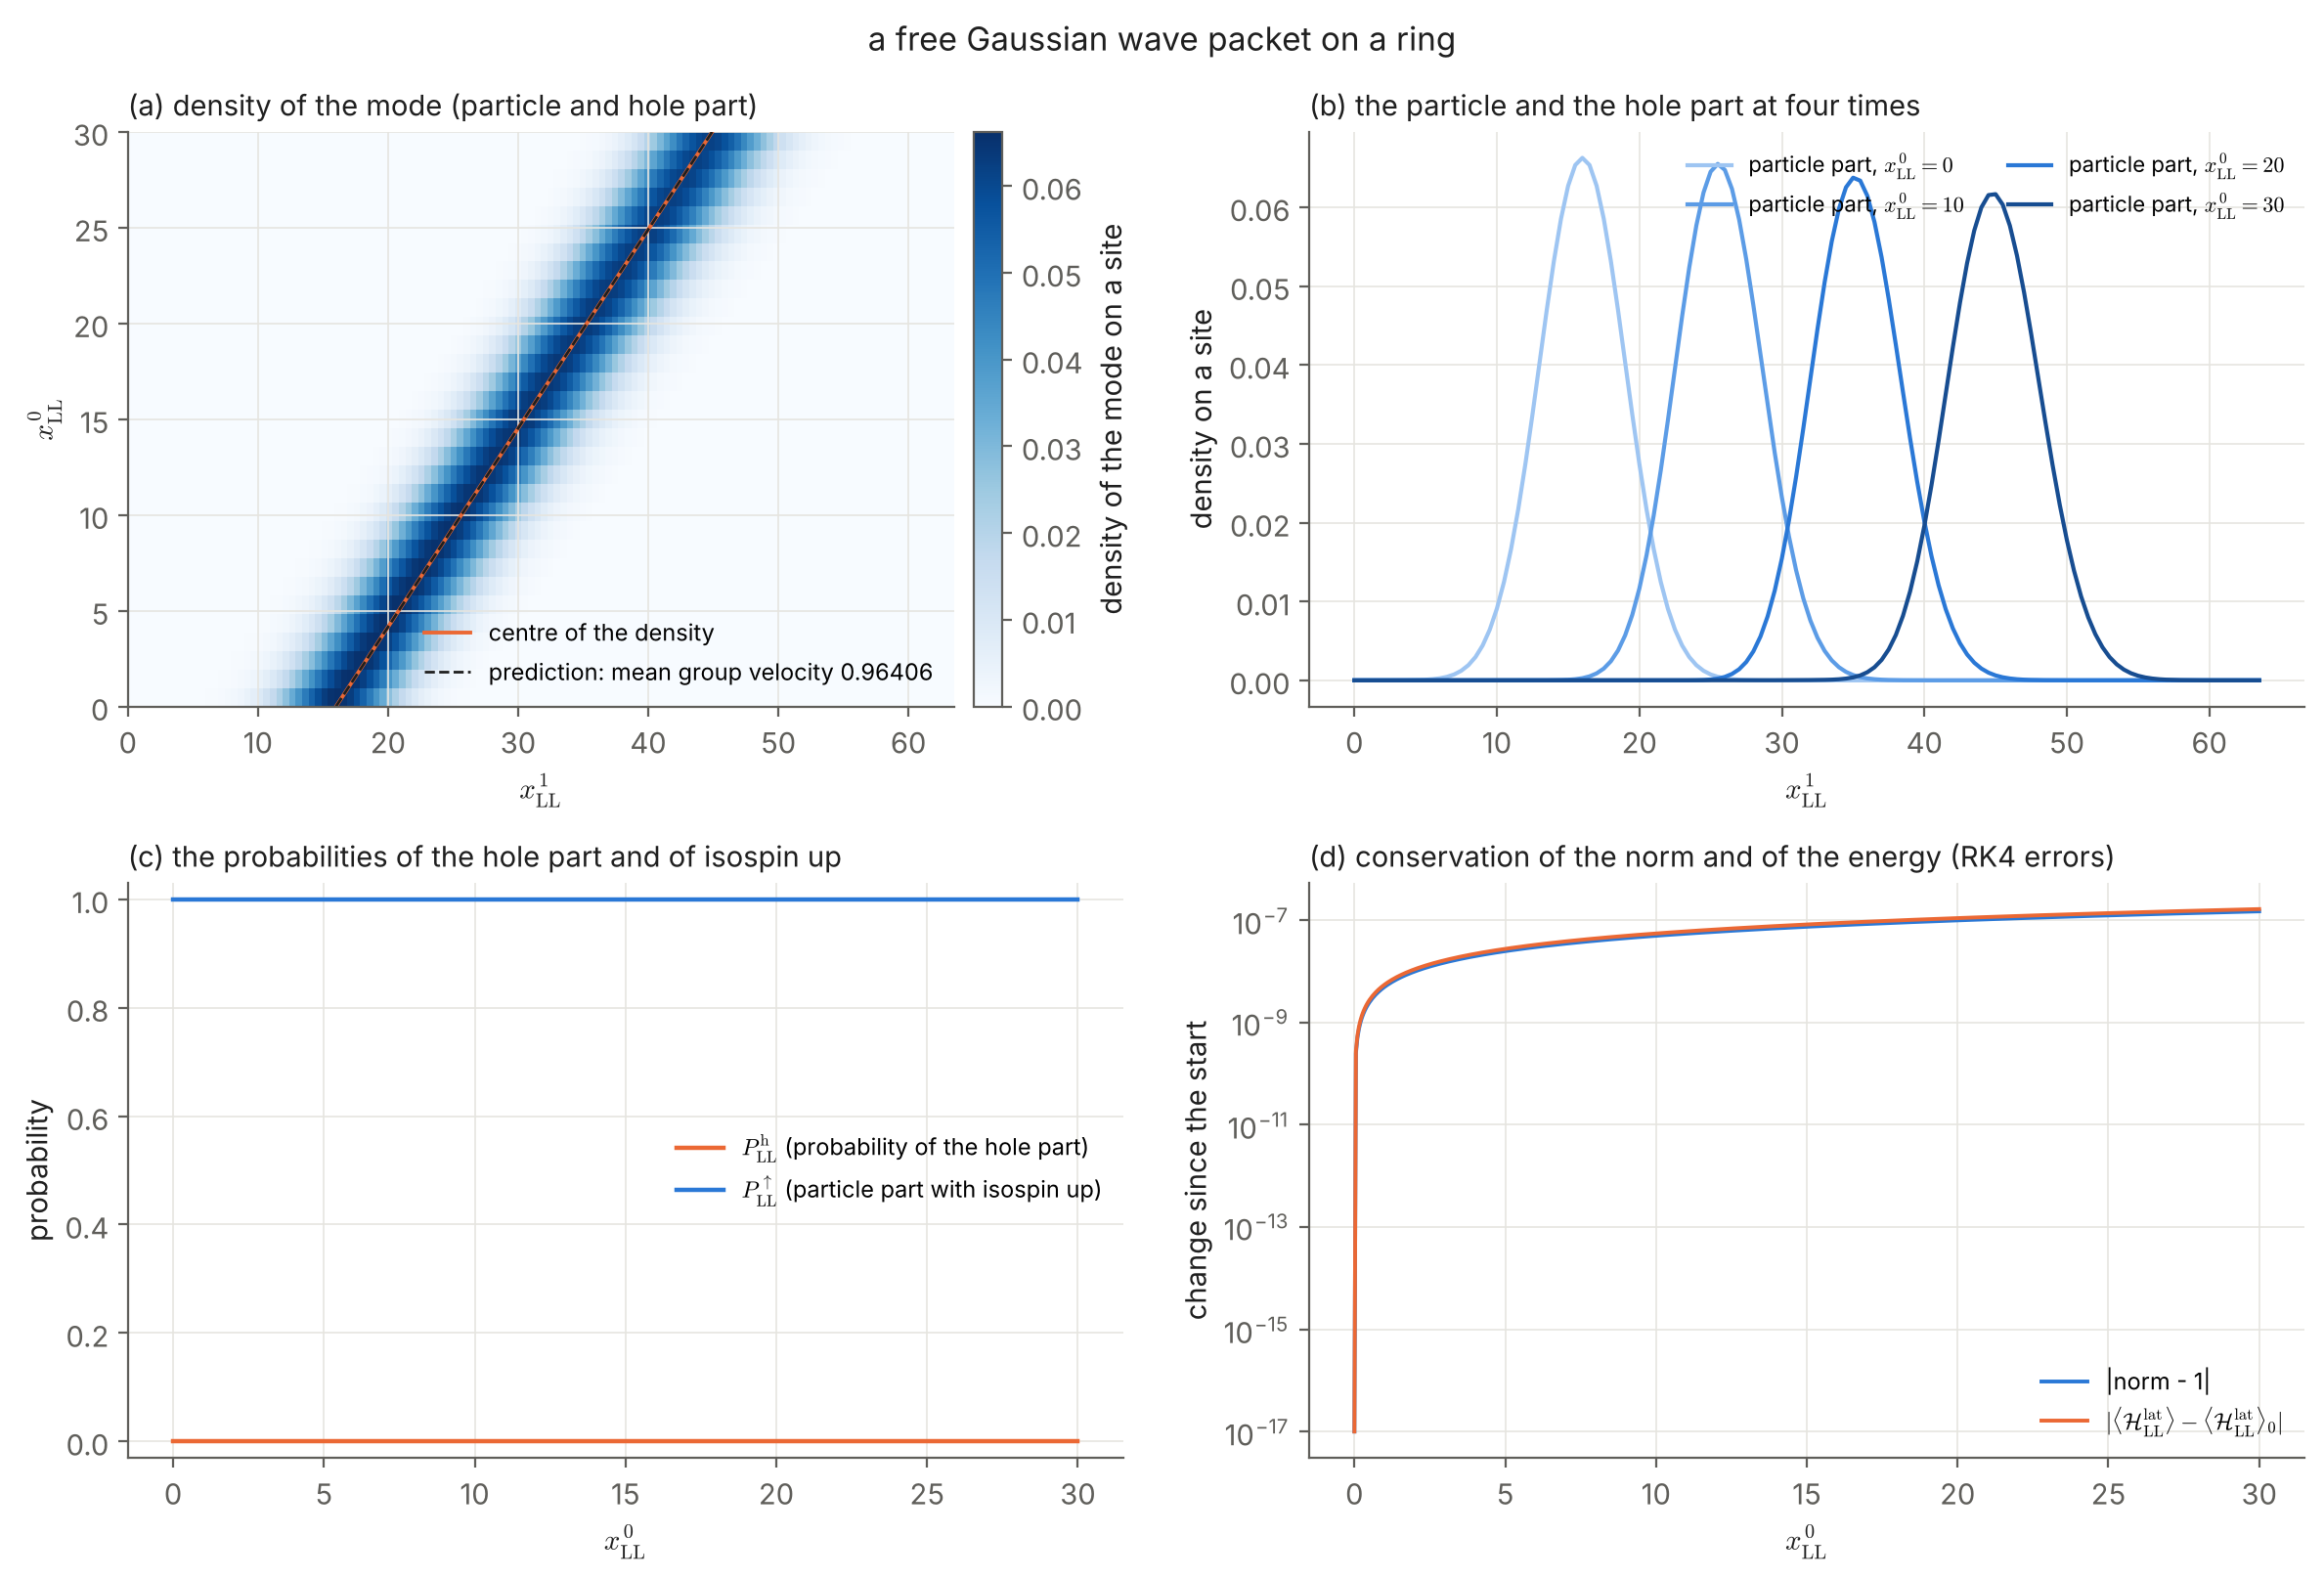
\includegraphics[width=1\textwidth,height=\textheight]{figures/fig_t2_py_packet_free.png}

\textbf{Figure 7.} The free wave packet (example \texttt{packet\_free},
check EX-1). (a) The packet moves through the ring without changing its
shape much; its centre (orange) lies on the dashed line of the predicted
mean group velocity 0.96406, the average of (4.7) over the momenta of
the packet; the two lines cannot be told apart (the difference is
\(8\times10^{-5}\) of the velocity). (b) The density at four times: the
packet broadens slowly by dispersion. (c) It stays a particle with
isospin up (\(P^{\rm h}_{\rm LL}=0\), \(P^\uparrow_{\rm LL}=1\)):
without fields nothing turns it. (d) The norm and the energy change by
less than \(2\times10^{-7}\), the size of the RK4 error for the energies
of the packet. Data: \texttt{test2/data/t2\_py\_packet\_free\_*}.

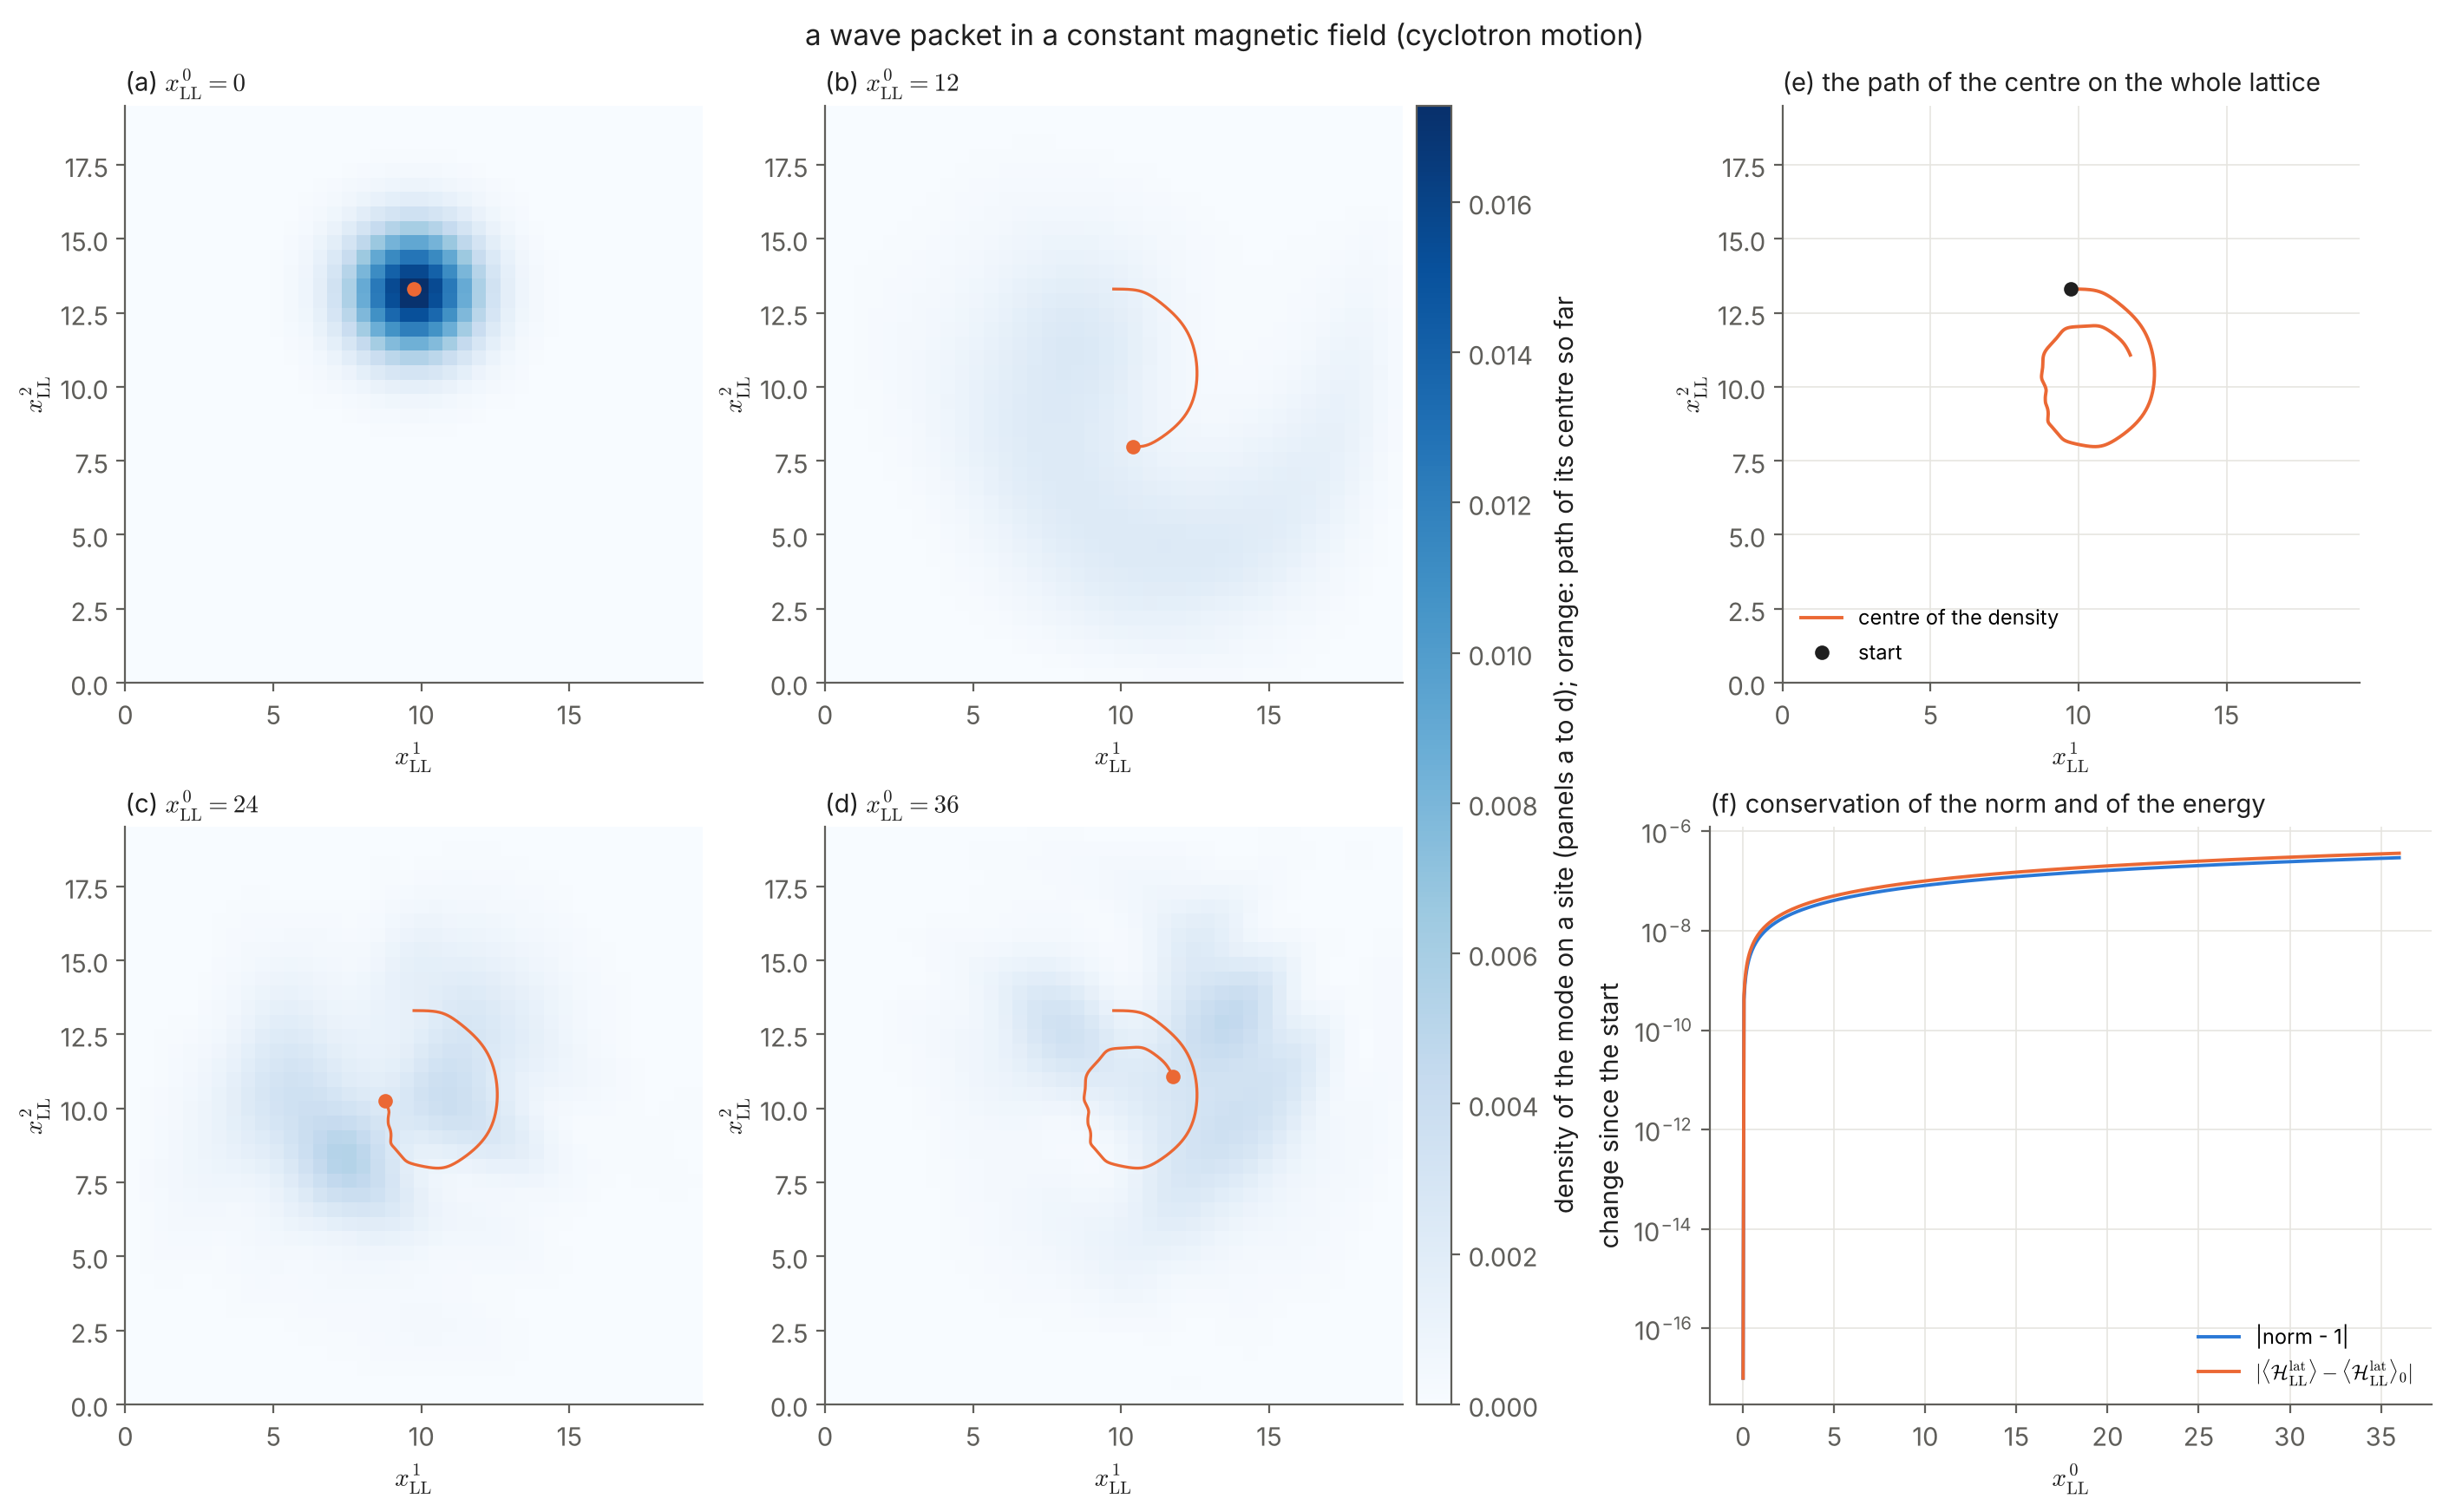
\includegraphics[width=1\textwidth,height=\textheight]{figures/fig_t2_py_cyclotron.png}

\textbf{Figure 8.} The packet in the magnetic field
\(\mathsf F^{\rm F}_{{\rm LL},12}=0.4\) (example \texttt{cyclotron},
check EX-2). (a) to (d) The density at four times and the path of the
centre so far: the packet turns, spreads around a ring, and part of it
comes back; it is a superposition of the Landau levels 0 to 3 of (3.32),
whose energy differences set the turning (Section 4.4). (e) The path of
the centre: bounded, far from the walls. (f) The norm and the energy are
conserved to \(4\times10^{-7}\). Data:
\texttt{test2/data/t2\_py\_cyclotron\_*}.

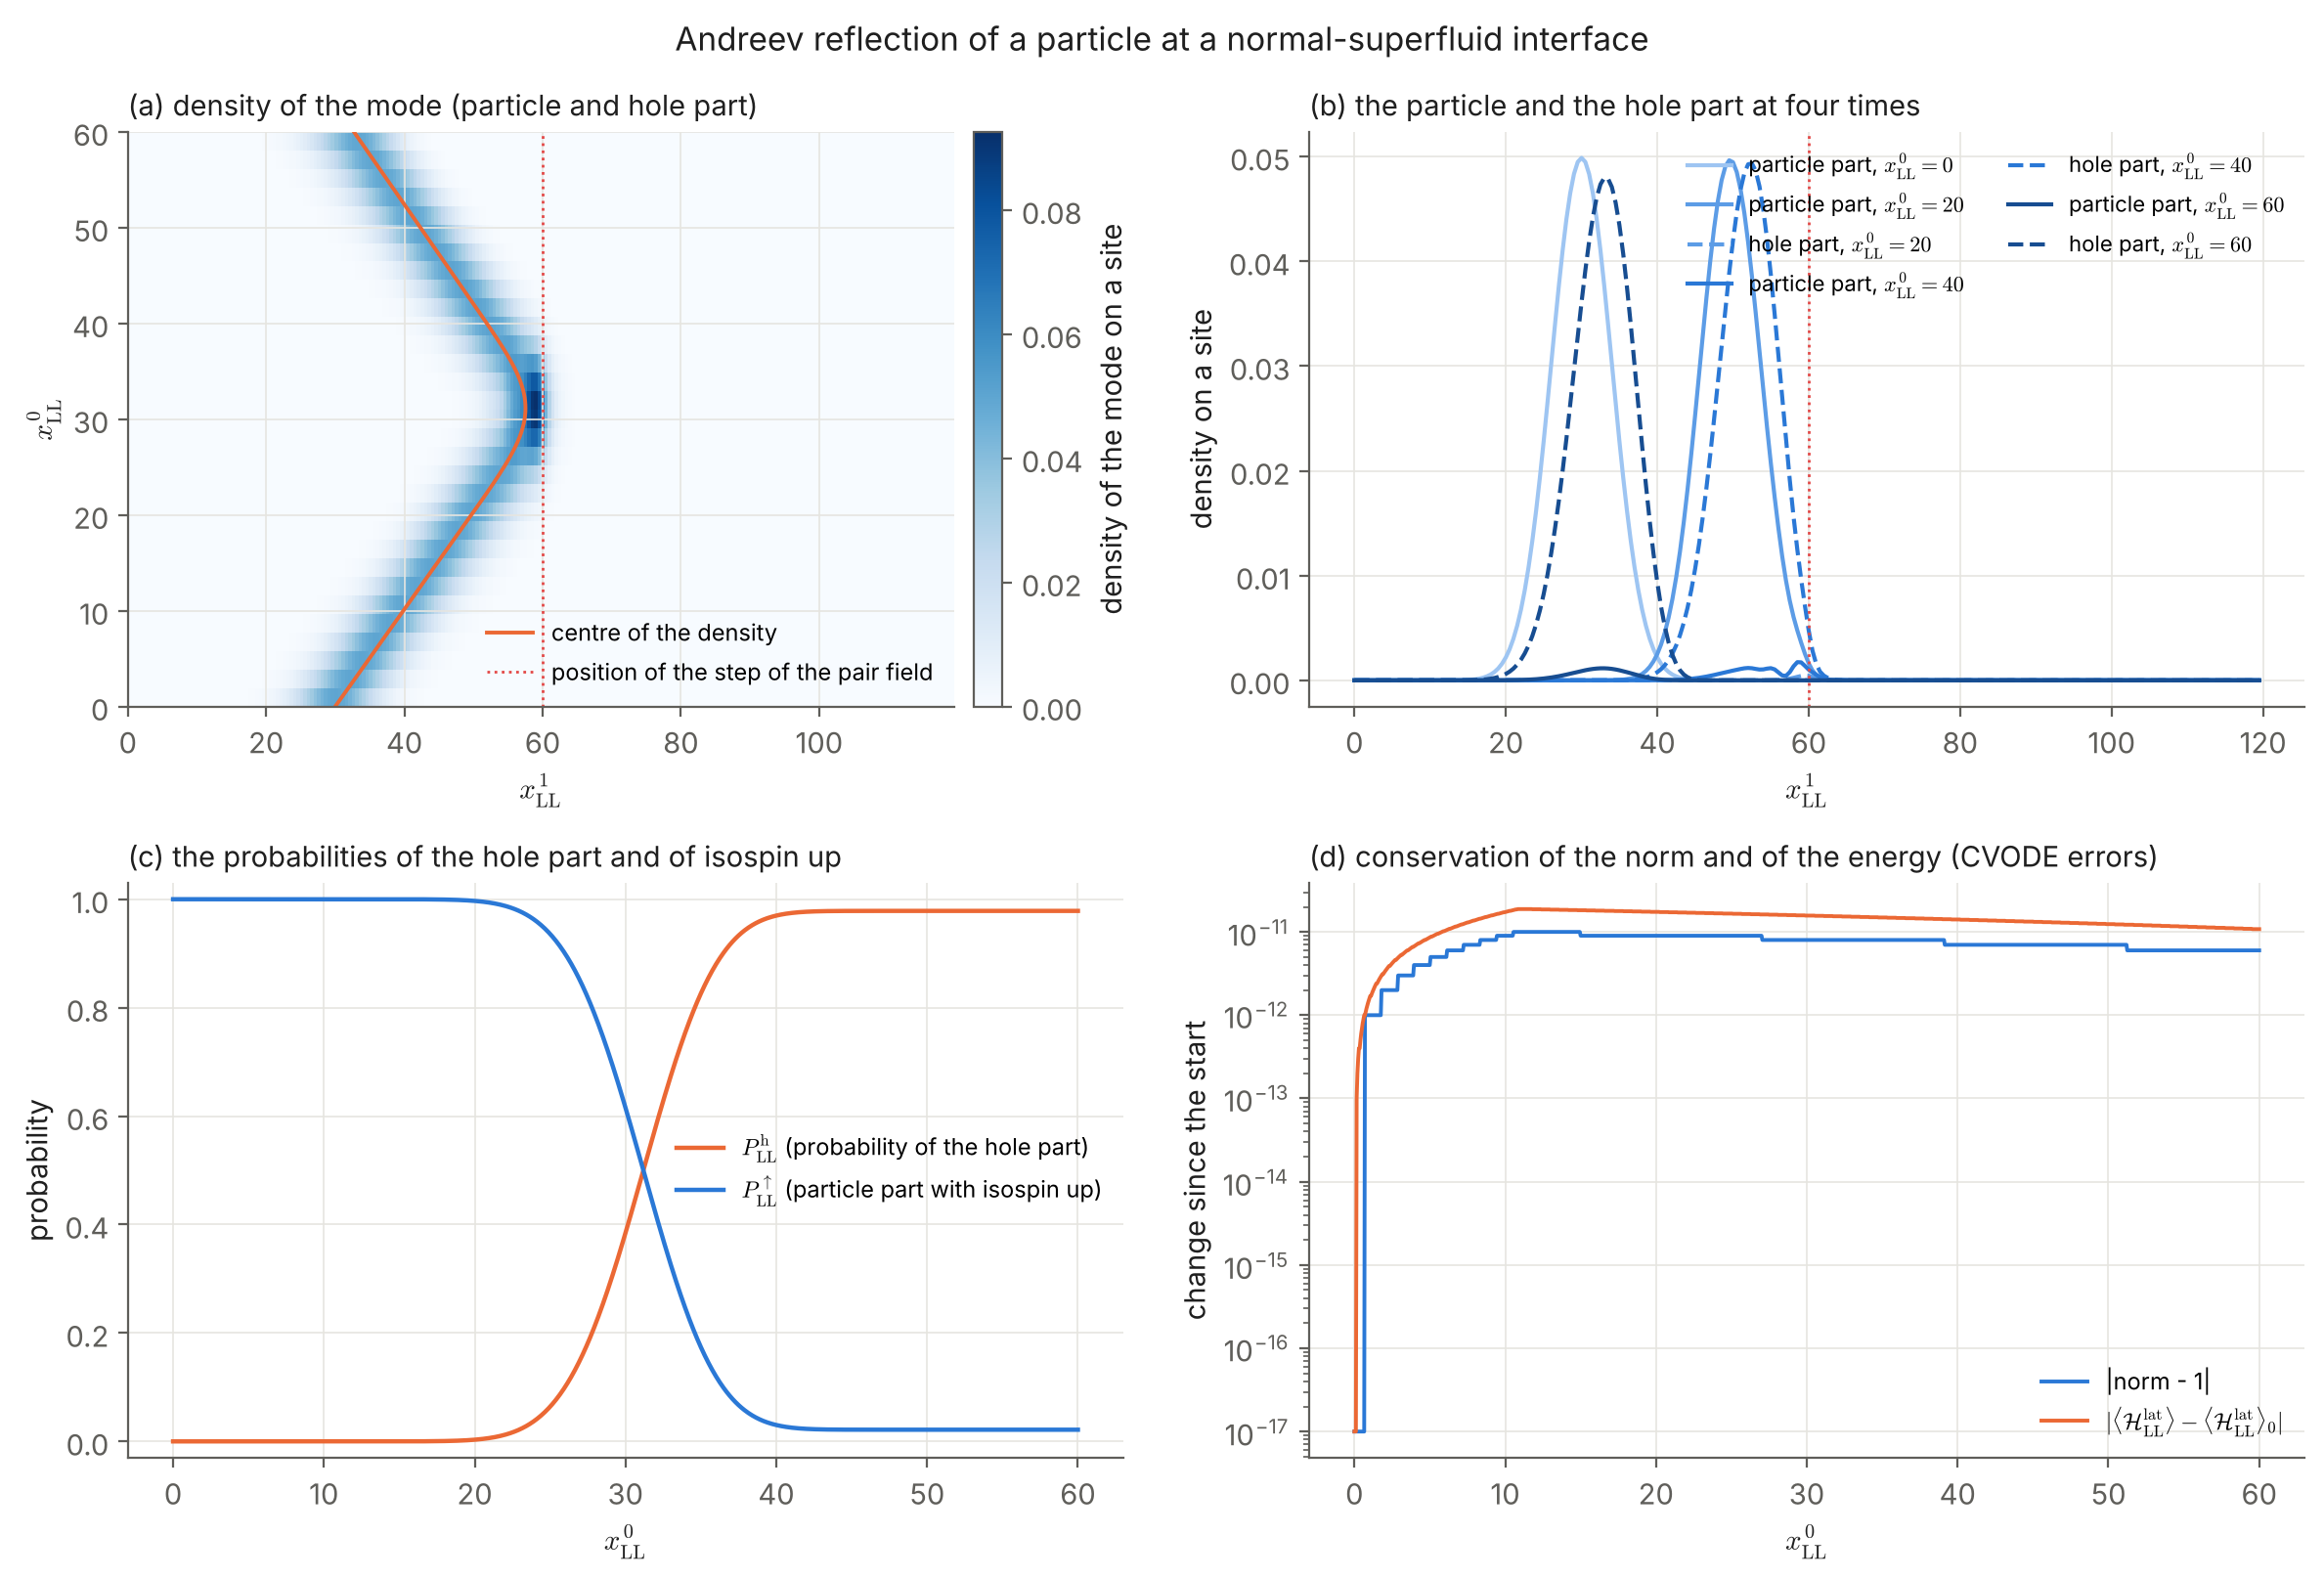
\includegraphics[width=1\textwidth,height=\textheight]{figures/fig_t2_py_andreev.png}

\textbf{Figure 9.} Andreev reflection (example \texttt{andreev}, check
EX-3). (a) A particle of energy 0.074, inside the gap 0.6 of the
superfluid region to the right of the dotted line, runs to the right,
turns before the interface and runs back. (b) At the times 20 and 40 the
incoming particle part (solid) and the outgoing hole part (dashed); at
60 only the hole part is left, with a small reflected particle part. (c)
The conversion: \(P^{\rm h}_{\rm LL}\) rises from 0 to 0.978 while the
packet is at the interface, and the particle part with isospin up falls
to 0.022. (d) The errors of the time stepping stay below
\(3\times10^{-9}\). Data: \texttt{test2/data/t2\_py\_andreev\_*}.

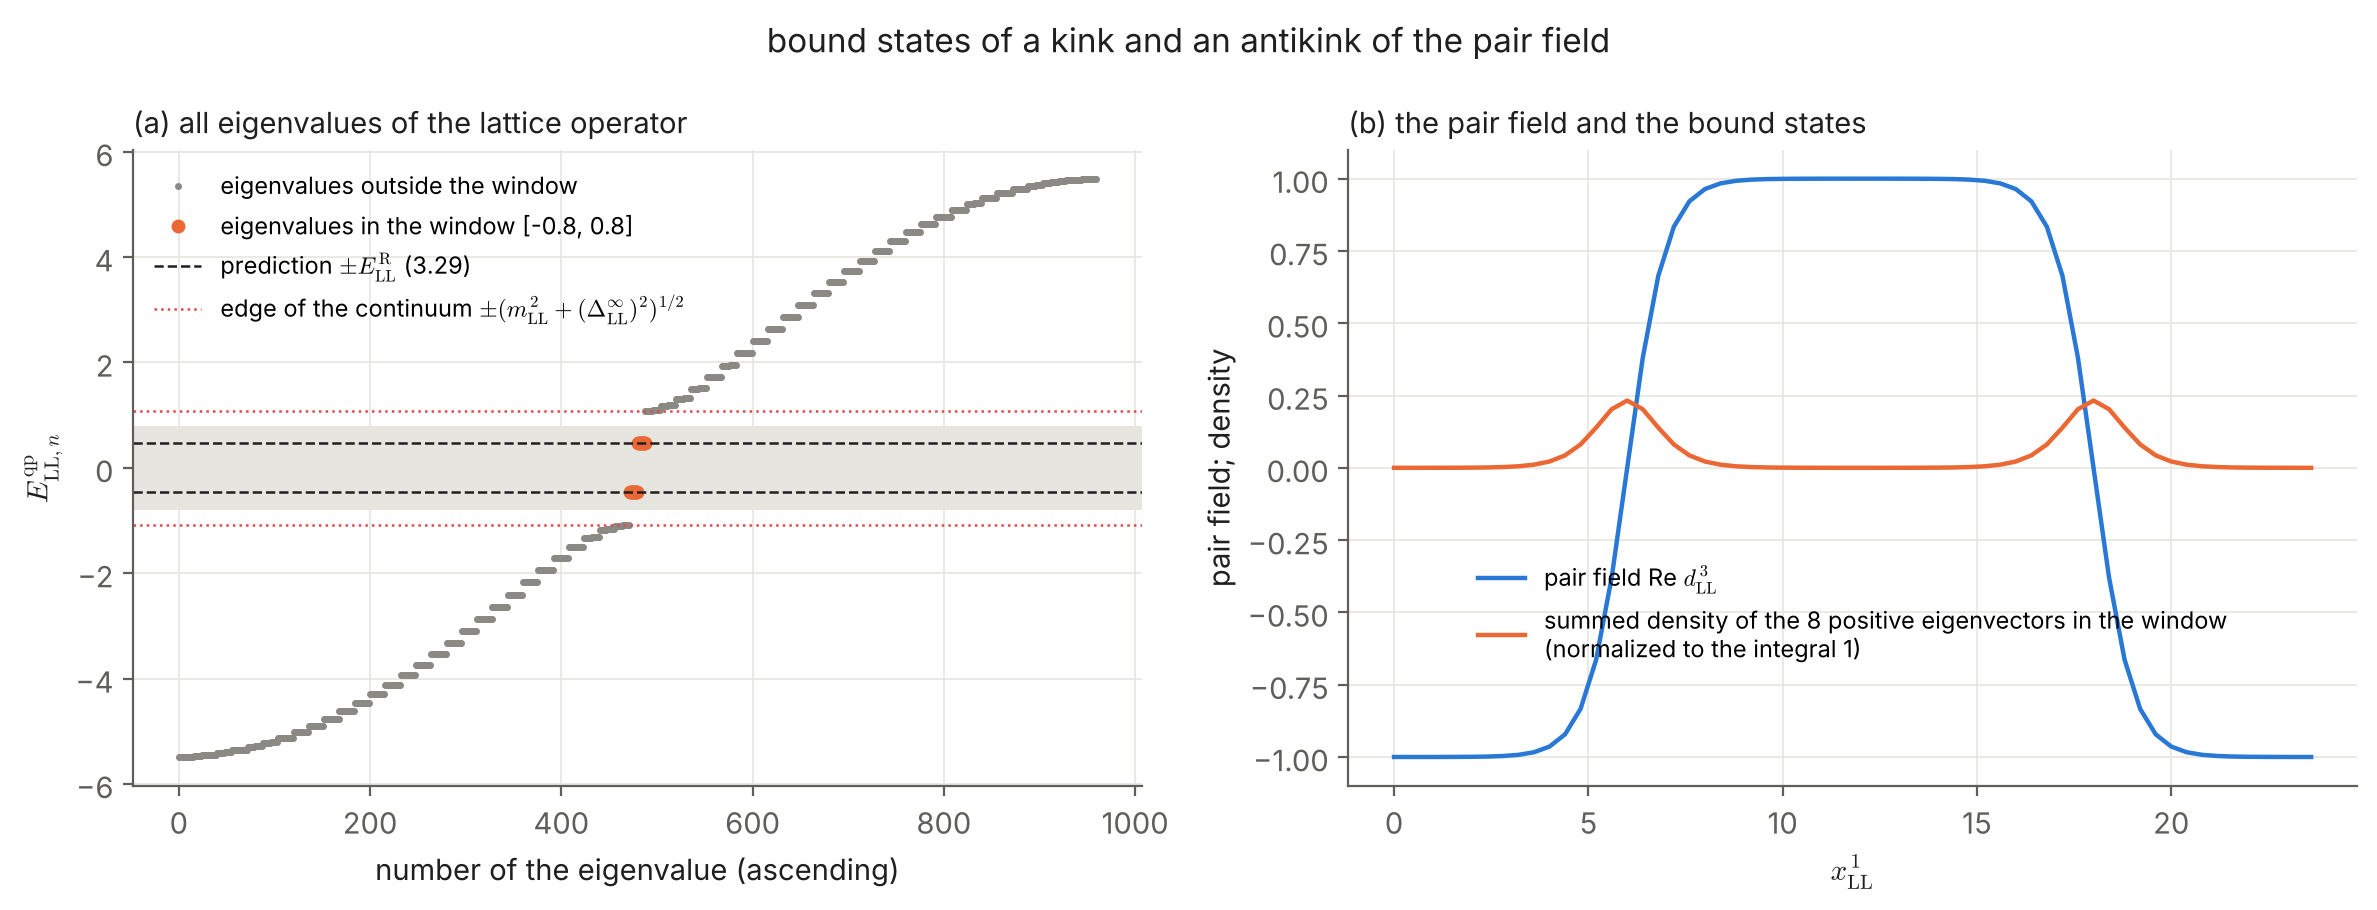
\includegraphics[width=1\textwidth,height=\textheight]{figures/fig_t2_py_kink_spectrum.png}

\textbf{Figure 10.} The kink and the antikink of the pair field on a
ring (example \texttt{kink\_spectrum}, check EX-4). (a) All 960
eigenvalues; inside the gap of the continuum (dotted,
\(\pm(m_{\rm LL}^2+(\Delta^\infty_{\rm LL})^2)^{1/2}\)) lie exactly 16,
on the predicted energies \(\pm E^{\rm R}_{\rm LL}\) of (3.29) (dashed)
within the bound of perturbation theory. (b) The pair field and the
summed density of the eight bound states of positive energy: they sit on
the two walls. Data: \texttt{test2/data/t2\_py\_kink\_spectrum\_*}.

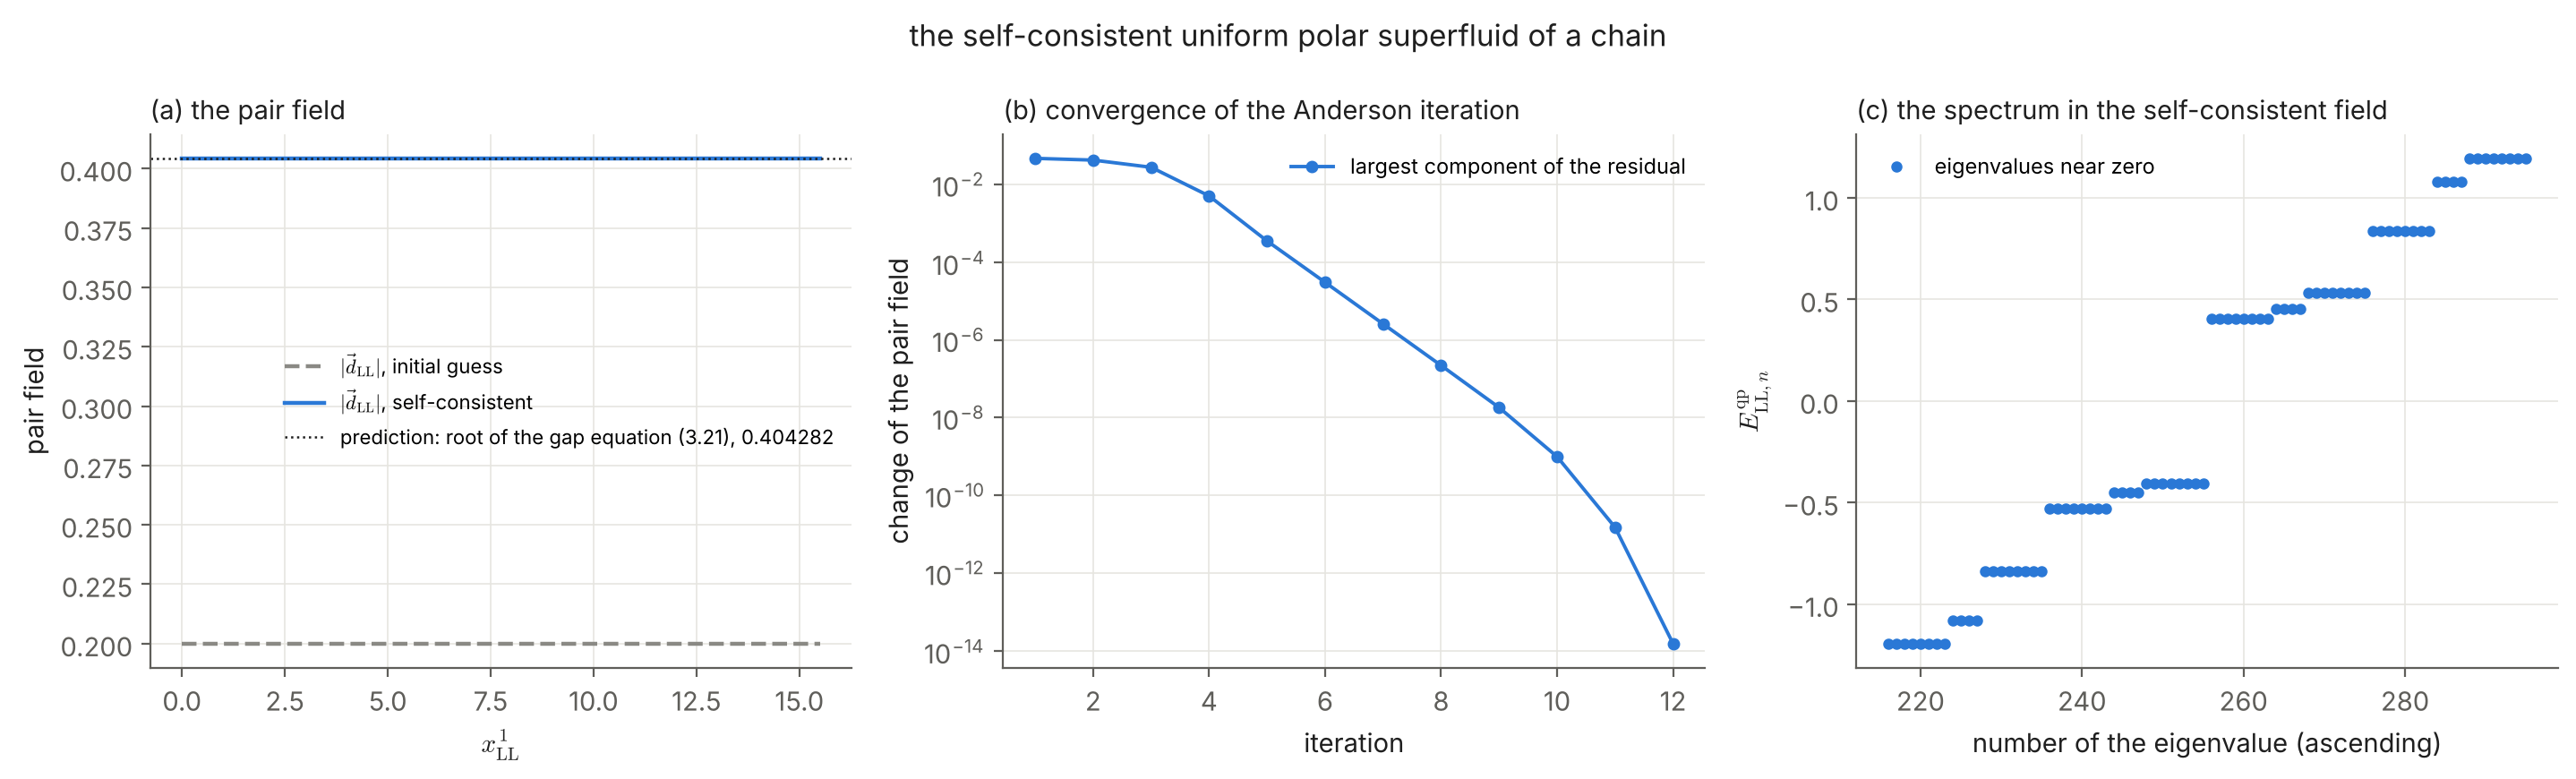
\includegraphics[width=1\textwidth,height=\textheight]{figures/fig_t2_py_ground_state.png}

\textbf{Figure 11.} The self-consistent uniform superfluid (example
\texttt{ground\_state}, check EX-5). (a) From the guess 0.2 (grey,
dashed) the iteration reaches the uniform
\(\lvert\vec d_{\rm LL}\rvert\) (blue) on the root of the lattice gap
equation (3.21) (dotted). (b) The Anderson iteration converges in 12
steps to \(10^{-14}\). (c) The eigenvalues near zero: the gap opens
around zero energy. Data: \texttt{test2/data/t2\_py\_ground\_state\_*}.

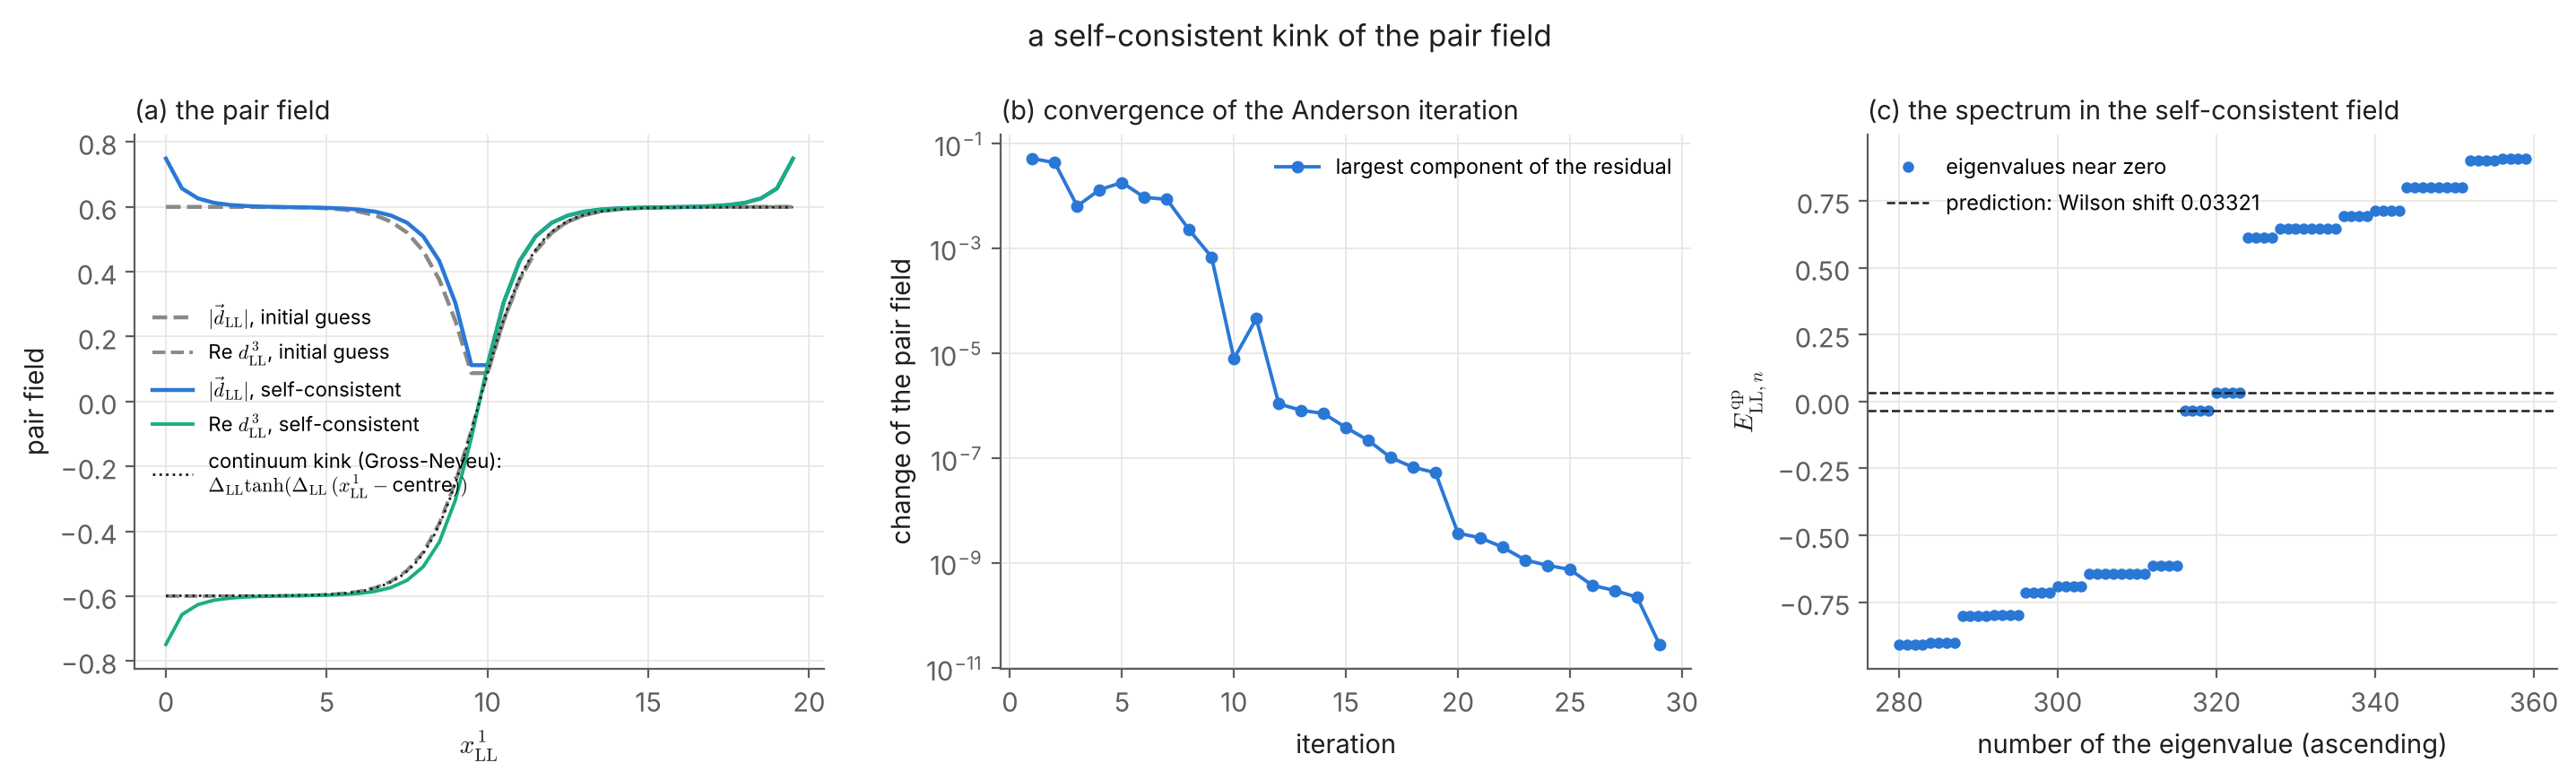
\includegraphics[width=1\textwidth,height=\textheight]{figures/fig_t2_py_kink_ground_state.png}

\textbf{Figure 12.} The self-consistent kink between two walls (example
\texttt{kink\_ground\_state}, check EX-6). (a) The guess (grey, dashed),
the self-consistent \(\mathrm{Re}\,d^3_{\rm LL}\) (aqua) and
\(\lvert\vec d_{\rm LL}\rvert\) (blue), and the continuum kink of the
Gross-Neveu model with the uniform gap of the same coupling (dotted):
the lattice kink is slightly steeper (the Wilson term), and the pair
field rises near the hard walls. (b) The convergence of the constrained
Anderson iteration. (c) The eight bound states, four at each sign, at
the energies \(\pm0.034\), next to the predicted first-order Wilson
shift (dashed); the continuum begins at 0.61. Data:
\texttt{test2/data/t2\_py\_kink\_ground\_state\_*}.

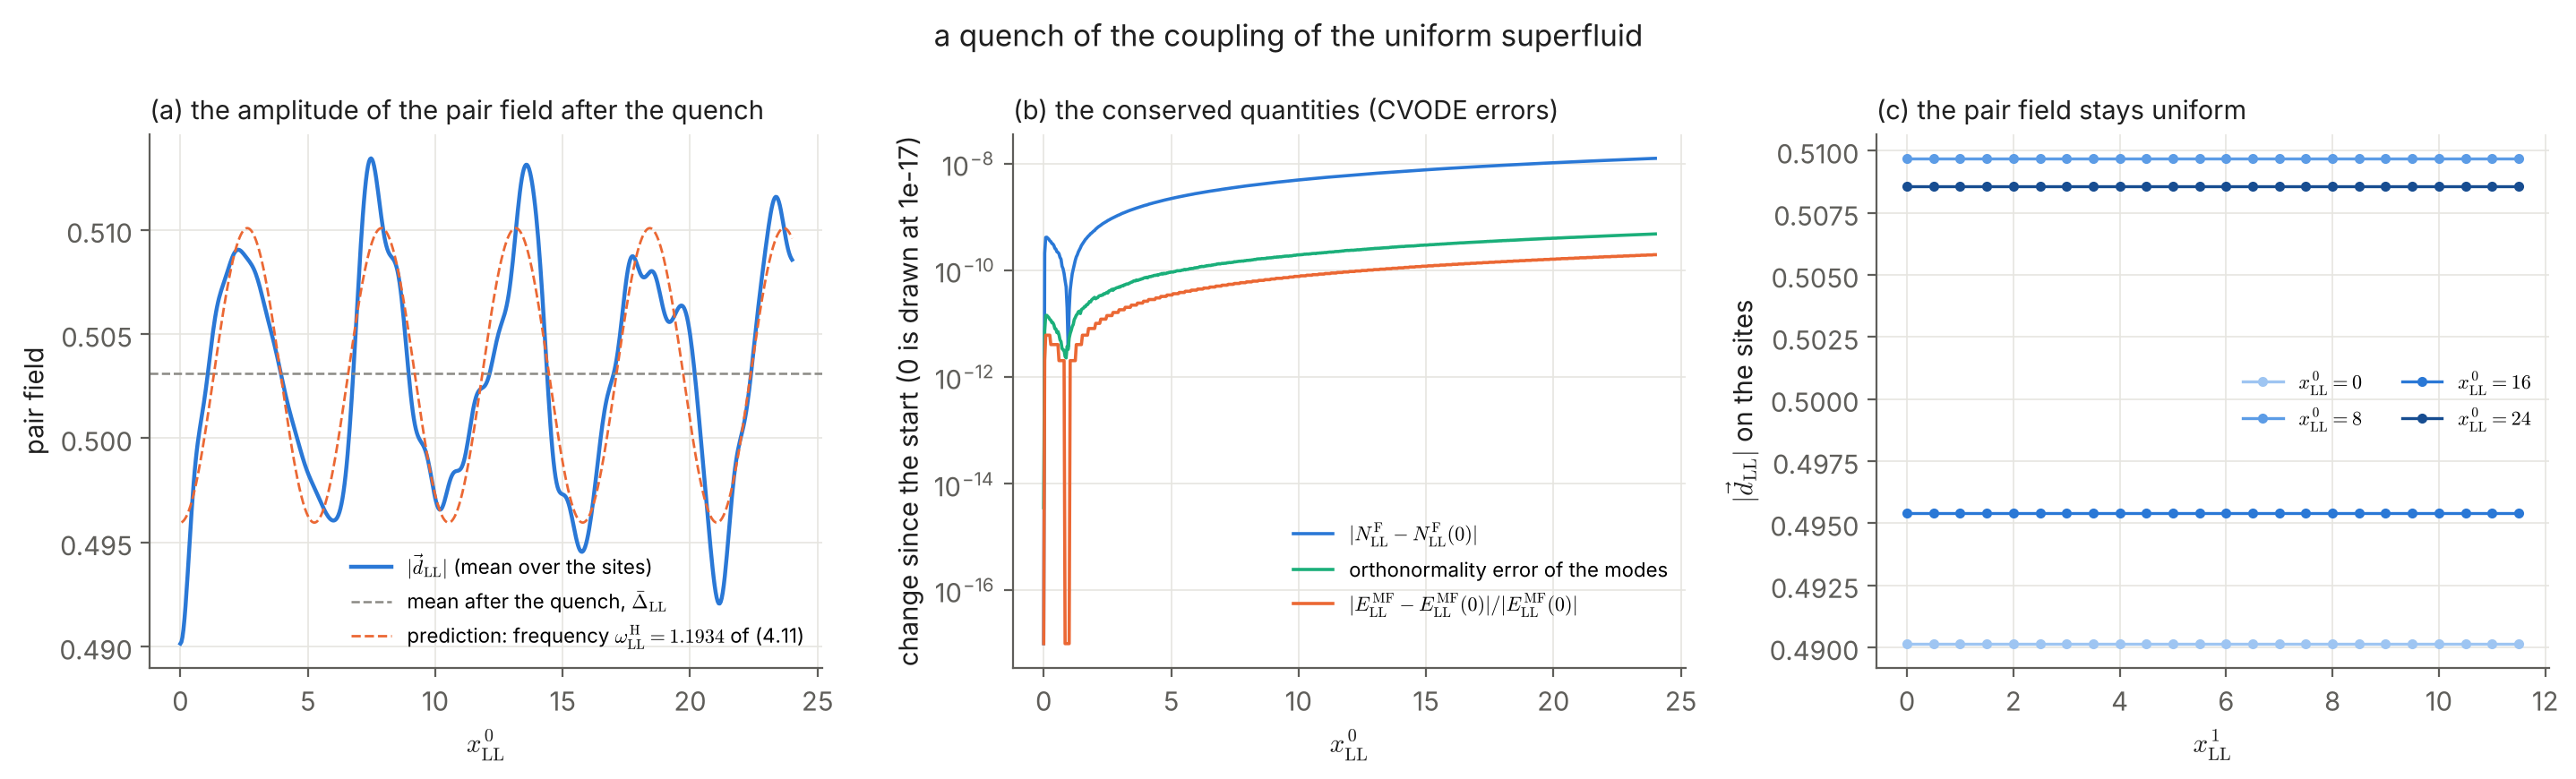
\includegraphics[width=1\textwidth,height=\textheight]{figures/fig_t2_py_quench.png}

\textbf{Figure 13.} The quench of the coupling from 0.45 to 0.455
(example \texttt{quench}, check EX-7). (a) The amplitude of the pair
field jumps at \(x^0_{\rm LL}=0\) (by the factor
\(G'_{\rm LL}/G_{\rm LL}\)) and then oscillates about its mean (grey);
the dashed curve is a sinusoid with the predicted frequency
\(\omega^{\rm H}_{\rm LL}\) of (4.11) (amplitude and phase fitted): the
dominant oscillation follows it, and weaker modes at other frequencies
are visible as well. (b) The fermion number changes by at most
\(2.4\times10^{-11}\) and the orthonormality of the modes by
\(1.2\times10^{-12}\) (rounding errors), while \(E^{\rm MF}_{\rm LL}\)
varies by a few parts in \(10^{6}\) without drift (the second-order
error of the midpoint rule). (c) The pair field stays uniform on all 24
sites. Data: \texttt{test2/data/t2\_py\_quench\_*}.

\hypertarget{discussion-3}{%
\subsection{5.4 Discussion}\label{discussion-3}}

\begin{itemize}
\tightlist
\item
  \textbf{What the plots prove.} Each figure puts the computed solution
  next to an independent prediction drawn from a different formula: the
  mean group velocity, the energies of the bound states, the root of the
  gap equation, the continuum kink and the Wilson shift, the frequency
  of the amplitude mode. Agreement is visible at a glance, and the
  numbers are in the reports of Appendix A.
\item
  \textbf{What the plots show beyond the checks.} The time scale of the
  Andreev conversion (the packet stays near the interface for a time of
  order \(1/\Delta_{\rm LL}\)), the spreading of the packet in the
  magnetic field into its Landau levels, the rise of the pair field near
  hard walls, and the weaker modes in the quench, which the
  single-frequency check does not test.
\item
  \textbf{Limits.} The program draws one solution at a time and chooses
  its panels by the task. For three active directions it draws the
  density summed over \(x^3_{\rm LL}\) in the plane of the first two
  coordinates (the full fields are in the data files); the profiles of
  the self-consistent pair field are drawn along \(x^1_{\rm LL}\).
\end{itemize}

\hypertarget{item-5-a-rust-program-that-solves-the-field-equations}{%
\section{6. Item {[}5{]}: a Rust program that solves the field
equations}\label{item-5-a-rust-program-that-solves-the-field-equations}}

\hypertarget{the-answer-in-brief-4}{%
\subsection{6.0 The answer in brief}\label{the-answer-in-brief-4}}

The program \texttt{t2\_solve} is the member \texttt{t2solve} of the
Cargo workspace \texttt{test2/rust} (pure Rust: the standard library and
the library \texttt{t2core} of the workspace, no downloaded crate; about
2700 commented lines in three files). It is built with
\texttt{cargo\ build\ -\/-release} and does everything the Python solver
of item {[}3{]} does, in the same way: it guides the user (a short guide
at the start, the complete guide with \texttt{-\/-guide}, seven examples
written on request), asks for the name of the input file, reads the same
input files (format \texttt{t2in\ 1}, the 50 keys of Section 4.2, with
the same checks and the same error messages), solves the four tasks with
the same methods (RK4 for \texttt{evolve}, the dense eigensolver for
\texttt{spectrum}, Anderson acceleration for \texttt{ground\_state}, the
implicit midpoint rule for \texttt{quench}), checks every run in the
same way, and writes the same output files with the same columns. Its
self-test compares its sparse lattice operator with the operator
\texttt{Lattice::apply} of \texttt{t2core}, which was written
independently for items {[}1{]} and {[}2{]} (5 checks). For the seven
examples, the Rust and the Python solutions agree number by number: the
solutions, spectra and time series to \(10^{-9}\), which is rounding
(check EX-8), and the checks EX-1 to EX-7 pass for the Rust solutions as
well (11 checks in all).

\hypertarget{installing-rust-and-building-the-program}{%
\subsection{6.1 Installing Rust and building the
program}\label{installing-rust-and-building-the-program}}

\textbf{Step 1: install the Rust toolchain} (once per computer). On
macOS or Linux, in a terminal:

\begin{verbatim}
curl --proto '=https' --tlsv1.2 -sSf https://sh.rustup.rs | sh
# answer 1 (the default installation), then open a new terminal window, or type:
source "$HOME/.cargo/env"
# check: both commands print a version number
rustc --version
cargo --version
\end{verbatim}

On Windows the installer \texttt{rustup-init.exe} from the web page of
the Rust project does the same; the commands below are then typed in
PowerShell (with \texttt{\textbackslash{}} in the paths, and
\texttt{t2\_solve.exe} for the program).

\textbf{Step 2: build.} From the folder Revision\_SuperLoop of the
repository:

\begin{verbatim}
cd test2/rust
cargo build --release
\end{verbatim}

Cargo compiles the library \texttt{t2core} and the three programs of the
workspace (\texttt{t2\_fields}, \texttt{t2\_analytic},
\texttt{t2\_solve}) with full optimization; the first build takes about
a minute, later builds only recompile what changed. No network access is
needed, because the workspace uses no external crate. The program is
then the file \texttt{test2/rust/target/release/t2\_solve}.

\textbf{Step 3: check the build} (from the folder Revision\_SuperLoop):

\begin{verbatim}
./test2/rust/target/release/t2_solve --selftest
\end{verbatim}

It prints five lines \texttt{{[}PASS{]}\ ...} and
\texttt{self-test:\ ALL\ PASS} (with the folder \texttt{test2/examples}
as a further argument it also compares its examples with the input files
of that folder).

\hypertarget{using-the-program}{%
\subsection{6.2 Using the program}\label{using-the-program}}

The commands are those of the Python solver, with
\texttt{./test2/rust/target/release/t2\_solve} in place of
\texttt{python3\ test2/python/t2\_solve.py} (all from the folder
Revision\_SuperLoop):

\begin{verbatim}
# the complete guide: what is solved, the boundary and initial conditions, every key
./test2/rust/target/release/t2_solve --guide
# the examples, and one of them written as an input file to start from
./test2/rust/target/release/t2_solve --examples
./test2/rust/target/release/t2_solve --example andreev my_problem.t2in
# solve an input file (the output files are named after it, in its folder)
./test2/rust/target/release/t2_solve my_problem.t2in
# the same with another name for the output files
./test2/rust/target/release/t2_solve my_problem.t2in --out results/run1
# without arguments: a short guide, then the question for the name of the input file
./test2/rust/target/release/t2_solve
# plot a solution with the Python plotter of item [4]
python3 test2/python/t2_plot.py my_problem
\end{verbatim}

In the dialogue the program answers \texttt{?} with the complete guide,
\texttt{examples} with the list of examples, \texttt{example\ NAME} by
writing the example as \texttt{NAME.t2in}, and a file name by solving
that file; \texttt{q} (or an empty line) ends it. An input file written
for one solver runs unchanged with the other, and both write the files
\texttt{NAME\_summary.txt}, \texttt{NAME\_series.csv},
\texttt{NAME\_fields.csv} and, for some tasks,
\texttt{NAME\_spectrum.csv} and \texttt{NAME\_iterations.csv} (Sections
4.3 and A.3). The exit status is 0 when every check of the run passes, 1
when a check fails, and 2 when the input is wrong.

\textbf{What the messages mean, and what to do.}

\begin{longtable}[]{@{}
  >{\raggedright\arraybackslash}p{(\columnwidth - 4\tabcolsep) * \real{0.2857}}
  >{\raggedright\arraybackslash}p{(\columnwidth - 4\tabcolsep) * \real{0.3571}}
  >{\raggedright\arraybackslash}p{(\columnwidth - 4\tabcolsep) * \real{0.3571}}@{}}
\toprule\noalign{}
\begin{minipage}[b]{\linewidth}\raggedright
message
\end{minipage} & \begin{minipage}[b]{\linewidth}\raggedright
meaning
\end{minipage} & \begin{minipage}[b]{\linewidth}\raggedright
what to do
\end{minipage} \\
\midrule\noalign{}
\endhead
\bottomrule\noalign{}
\endlastfoot
\texttt{unknown\ key\ \textquotesingle{}pair\_widht\textquotesingle{}\ (did\ you\ mean\ pair\_width?)}
& a misspelt key & correct the name \\
\texttt{the\ task\ \textquotesingle{}quench\textquotesingle{}\ needs\ the\ key\ \textquotesingle{}quench\_coupling\textquotesingle{}}
& a key that the task requires is missing & add it (Section 4.2) \\
\texttt{dt\ Hbound\ =\ 3.1\ exceeds\ 2.5:\ choose\ time\_step\ below\ 0.4}
& the time step is too long for RK4 to be stable & use a smaller
\texttt{time\_step} \\
\texttt{dt\ Hbound\ =\ 1.3\ exceeds\ 1:\ ...} (quench) & the fixed-point
iteration of the implicit midpoint rule would not converge & use a
smaller \texttt{time\_step} \\
\texttt{...\ must\ not\ exceed\ 6000} & the dense diagonalization of
\texttt{spectrum}, \texttt{ground\_state} and \texttt{quench} is limited
to 375 sites & use fewer sites \\
\texttt{a\ magnetic\ field\ needs\ \textquotesingle{}wall\textquotesingle{}\ in\ direction\ 1}
& the Landau gauge grows along \(x^1_{\rm LL}\) & make direction 1 a
wall \\
\texttt{{[}FAIL{]}\ the\ self-consistent\ ...\ converged} & the
iteration did not reach \texttt{tolerance} & raise
\texttt{max\_iterations}, lower \texttt{mixing}, or start from a better
\texttt{pair} \\
\end{longtable}

\hypertarget{how-the-program-is-built}{%
\subsection{6.3 How the program is
built}\label{how-the-program-is-built}}

Three source files in \texttt{test2/rust/t2solve/src}:

\begin{itemize}
\tightlist
\item
  \texttt{input.rs}: the table of the 50 keys (name, kind, default,
  meaning), the keys that each task requires, and the seven examples,
  all copied from the Python solver (the self-test checks that the
  examples written by both programs are identical), the reading and
  checking of an input file, and the guide;
\item
  \texttt{ops.rs}: the lattice and the coordinates of the sites; the
  gauge potentials of each site (constant, from the gauge file, the
  Landau gauge, the pulse) and from them the link matrices (2.34) and
  the potential matrices, with the closed forms \texttt{link} and
  \texttt{potential} of \texttt{t2core}; the pair field of the key
  \texttt{pair} (the random field with the generator SplitMix64 of
  \texttt{t2core}, which the Python solver reproduces exactly); the
  sparse lattice operator (2.36) in compressed rows, assembled from the
  same \(8\times8\) blocks as in Section 4.3 (blocks between the same
  pair of sites are added); the pair expectation of (4.1); the wave
  packet (4.2) with the projection on its branch through the discrete
  Fourier transform along each periodic direction; the exact mean
  velocity of a free packet; the centre of a density; the root of the
  gap equation (3.21); the frequency fit; and a small linear solver for
  the Anderson step;
\item
  \texttt{main.rs}: the four tasks, the summary and the data files, the
  self-test, the dialogue and the command line.
\end{itemize}

The methods are those of Section 4.3, step by step: RK4 with the stages
at the times \(x^0_{\rm LL}\), \(x^0_{\rm LL}+\ell^{\rm t}_{\rm LL}/2\)
and \(x^0_{\rm LL}+\ell^{\rm t}_{\rm LL}\); the Anderson iteration (4.4)
with the memory 6, the normal equations with the regularization
\(10^{-12}\) times their trace, and Gaussian elimination with partial
pivoting; the implicit midpoint rule (4.6) with the explicit Euler start
and the stopping change \(10^{-14}\). The dense eigenproblems are solved
by the eigensolver of \texttt{t2core} (Householder reduction and the
implicit QL algorithm, check GS-11 of item {[}1{]}). Two things
necessarily differ from the Python solver, and neither changes a result:

\begin{itemize}
\tightlist
\item
  \emph{The eigenvectors inside a degenerate eigenspace.} Two
  eigensolvers choose different bases of an eigenspace of a repeated
  eigenvalue (for example the four bound states of each wall at the same
  energy). Every quantity that the solvers compute from eigenvectors is
  independent of that choice: the pair expectation of (4.1) and the
  fermion number are sums over all occupied modes (unchanged by a
  unitary mixing of them), the self-consistent evolution (4.6) acts on
  each mode separately and computes the pair field from the sum, and the
  task \texttt{spectrum} writes the densities summed over each group of
  degenerate eigenvalues. (The only exception is
  \texttt{initial\ =\ eigenmode} with a degenerate eigenvalue, whose
  initial mode depends on the eigensolver; the guide says so.)
\item
  \emph{The arithmetic.} The sums are formed in a different order, so
  the last digits differ by rounding; in the time stepping and in the
  iterations these differences are carried along but not amplified much.
\end{itemize}

\hypertarget{the-results-and-the-comparison-with-the-python-solver}{%
\subsection{6.4 The results, and the comparison with the Python
solver}\label{the-results-and-the-comparison-with-the-python-solver}}

The program solves the seven examples of Section 4.4; all checks of its
runs pass, and the program \texttt{t2\_examples\_check.py}, applied to
its outputs (prefix \texttt{t2\_rs\_} in \texttt{test2/data}), confirms
EX-1 to EX-7 with the same numbers as for the Python solutions (Appendix
A.2d). The check \textbf{EX-8} compares the 18 output files of the two
solvers column by column:

\begin{longtable}[]{@{}
  >{\raggedright\arraybackslash}p{(\columnwidth - 4\tabcolsep) * \real{0.4286}}
  >{\raggedright\arraybackslash}p{(\columnwidth - 4\tabcolsep) * \real{0.1429}}
  >{\raggedright\arraybackslash}p{(\columnwidth - 4\tabcolsep) * \real{0.4286}}@{}}
\toprule\noalign{}
\begin{minipage}[b]{\linewidth}\raggedright
quantities
\end{minipage} & \begin{minipage}[b]{\linewidth}\raggedright
largest difference
\end{minipage} & \begin{minipage}[b]{\linewidth}\raggedright
origin
\end{minipage} \\
\midrule\noalign{}
\endhead
\bottomrule\noalign{}
\endlastfoot
densities, pair fields, spectra (all examples) & \(10^{-14}\) or less &
rounding in the operator and the eigensolvers \\
time series of \texttt{evolve} (norm, energy, probabilities, centre) &
\(10^{-11}\) & rounding, carried through 600 to 1200 RK4 steps \\
time series of \texttt{quench} (\(\lvert\vec d_{\rm LL}\rvert\),
\(N^{\rm F}_{\rm LL}\), \(E^{\rm MF}_{\rm LL}\), orthonormality) &
\(10^{-9}\) (in \(E^{\rm MF}_{\rm LL}\approx491\), relative
\(2\times10^{-12}\)) & rounding, carried through 600 steps of (4.6) \\
histories of the Anderson iteration & \(2\times10^{-7}\) (the same
numbers of iterations) & rounding, amplified by the least-squares step
near convergence \\
\end{longtable}

The allowed differences are \(10^{-7}\) for the solutions and
\(10^{-5}\) for the iteration histories: the intermediate iterates of
the Anderson method depend on rounding through its least-squares step,
whose matrix becomes nearly singular when the residuals become small,
but the fixed point, which is what the iteration computes, agrees to
\(10^{-15}\) (the self-consistent pair fields of the files
\texttt{\_fields.csv}). The two programs were written independently in
the sense that matters: the Rust program assembles the operator from the
formulas of (2.36) and is checked against \texttt{Lattice::apply} of
\texttt{t2core}, while the Python program assembles it in NumPy and is
checked against its own site-by-site loop; their agreement to
\(10^{-14}\) on the same problems tests both.

Computing times on one processor core (the computer that built this
document), in seconds:

\begin{longtable}[]{@{}lll@{}}
\toprule\noalign{}
example & Python & Rust \\
\midrule\noalign{}
\endhead
\bottomrule\noalign{}
\endlastfoot
\texttt{packet\_free} & 0.10 & 0.06 \\
\texttt{andreev} & 0.33 & 0.27 \\
\texttt{cyclotron} & 1.6 & 1.4 \\
\texttt{kink\_spectrum} & 0.9 & 2.7 \\
\texttt{ground\_state} & 1.7 & 5.0 \\
\texttt{kink\_ground\_state} & 7.4 & 24 \\
\texttt{quench} (time stepping) & 50 & 25 \\
\end{longtable}

The Rust program is faster where the work is its own loops (the time
stepping), and slower for the dense eigenproblems, where NumPy calls the
optimized LAPACK library; the eigensolver of \texttt{t2core} is a plain
implementation of the textbook method.

\hypertarget{discussion-4}{%
\subsection{6.5 Discussion}\label{discussion-4}}

\begin{itemize}
\tightlist
\item
  \textbf{Why a second solver.} Two programs in two languages, with two
  eigensolvers and two independent checks of the lattice operator, that
  agree to rounding on every example, make an error in the formulation
  or in the code very unlikely: an error would have to be made in the
  same way twice.
\item
  \textbf{What the Rust program adds.} It runs without Python and
  without any library outside the repository, and it is the faster of
  the two for long time evolutions.
\item
  \textbf{Limits.} The same as those of the Python solver (Section 4.5):
  external gauge fields, and the dense diagonalization of the
  self-consistent tasks (here also its speed).
\end{itemize}

\hypertarget{appendix-a.-provenance-programs-commands-reports-data-figures}{%
\section{Appendix A. Provenance: programs, commands, reports, data,
figures}\label{appendix-a.-provenance-programs-commands-reports-data-figures}}

\hypertarget{a.1-how-to-reproduce-everything}{%
\subsection{A.1 How to reproduce
everything}\label{a.1-how-to-reproduce-everything}}

From the folder Revision\_SuperLoop of the repository:

\begin{verbatim}
# 1. the checks GS-1 to GS-16 of item [1], the explicit matrices and equations, the data of Figures 1 and 2
cd test2/rust && cargo build --release && ./target/release/t2_fields && cd ../..
# 2. the checks AS-1 to AS-10 of item [2] (the analytic solutions) and the data of Figures 3 to 6
cd test2/rust && cargo build --release && ./target/release/t2_analytic && cd ../..
# 3. Figures 1 to 6 (test2/figures/fig_t2_*.pdf and .png)
python3 test2/python/make_t2_figures.py
# 4. item [3]: the self-test of the Python solver, the seven examples, the table of the keys, the checks EX-1 to EX-7
python3 test2/python/t2_solve.py --selftest test2/data/t2_py_selftest_checks.txt
for e in packet_free cyclotron andreev kink_spectrum ground_state kink_ground_state quench; do
  python3 test2/python/t2_solve.py test2/examples/$e.t2in --out test2/data/t2_py_$e; done
python3 test2/python/t2_solve.py --keys-md test2/data/t2_py_fragments.md
python3 test2/python/t2_examples_check.py test2/data/t2_py
# 5. item [4]: Figures 7 to 13, the plots of the seven solutions (test2/figures/fig_t2_py_*.pdf and .png)
for e in packet_free cyclotron andreev kink_spectrum ground_state kink_ground_state quench; do
  python3 test2/python/t2_plot.py test2/data/t2_py_$e --out test2/figures/fig_t2_py_$e; done
# 6. item [5]: the Rust solver (build, self-test, the seven examples) and the comparison with the Python solutions (EX-8)
cd test2/rust && cargo build --release && cd ../..
./test2/rust/target/release/t2_solve --selftest test2/data/t2_rs_selftest_checks.txt test2/examples
for e in packet_free cyclotron andreev kink_spectrum ground_state kink_ground_state quench; do
  ./test2/rust/target/release/t2_solve test2/examples/$e.t2in --out test2/data/t2_rs_$e; done
python3 test2/python/t2_examples_check.py test2/data/t2_rs test2/data/t2_py
# 7. everything of the folder Revision_SuperLoop, all checks and all documents, with one verdict ("ALL PASS")
bash code/scripts/check_all.sh
\end{verbatim}

The program \texttt{t2\_fields} runs in about 20 seconds,
\texttt{t2\_analytic} in about 5 seconds, the seven examples of item
{[}3{]} together in about 70 seconds (the quench 50 seconds), the Rust
solver of item {[}5{]} in about 60 seconds, all on one processor core.

Requirements: a Rust toolchain (edition 2021); Python 3 with NumPy,
SciPy and Matplotlib; for the documents pandoc (2.11 or later), XeLaTeX
and latexmk, the DejaVu fonts and the Latin Modern Math font. The Rust
programs of the folder test2 use no external crate.

\hypertarget{a.2-the-programs-of-items-1-and-2}{%
\subsection{A.2 The programs of items {[}1{]} and
{[}2{]}}\label{a.2-the-programs-of-items-1-and-2}}

The Cargo workspace \texttt{test2/rust} has four members (the fourth,
\texttt{t2solve}, is the solver of item {[}5{]}, Appendix A.2d):

\begin{itemize}
\tightlist
\item
  \texttt{t2core} (library): complex numbers and matrices, the Hermitian
  eigensolver, the super-loop operators as matrices (\texttt{model.rs}:
  \(M_{\rm LL}\), the frame, the Dirac matrices, \(\mathsf S_{\rm LL}\),
  \(\mathsf s_{\rm LL}\), \(T^\iota_{\rm LL}\),
  \(\mathsf K^\iota_{\rm LL}\), \(\mathsf P_{\rm LL}\),
  \(\psi'_{\rm LL}\), the Cayley-Dickson product), the lattice operator
  (\texttt{lattice.rs}) and exact symbolic linear forms for printing
  formulas (\texttt{sym.rs});
\item
  \texttt{t2fields} (program \texttt{t2\_fields}): the checks GS-1 to
  GS-16, the explicit matrices and component equations of Section 2
  (written into \texttt{test2/data/t2\_fragments.md}, from which this
  document takes them), and the data of Figures 1 and 2;
\item
  \texttt{t2analytic} (program \texttt{t2\_analytic}): the checks AS-1
  to AS-10 of the analytic solutions of Section 3 and the data of
  Figures 3 to 6. It applies the lattice operator of \texttt{t2core}
  (\texttt{lattice.rs}), the routine that the solvers use, to the
  analytic solutions, so that every analytic solution is also a test of
  that code. For item {[}2{]} the library received the RK4 step of the
  lattice equations (\texttt{Lattice::rk4\_step}), the matrix of the
  free lattice operator on a plane wave (\texttt{h\_lat\_plane}), and a
  faster form of the Hermitian eigensolver (the same method; check GS-11
  still passes).
\end{itemize}

Together they have 7135 lines of commented Rust in 12 files. Arithmetic:
double precision; each check names its tolerance; random numbers from a
fixed seed, so that every run gives the same output.

The report, verbatim (\texttt{test2/data/t2\_fields\_checks.txt}). It
writes the symbols with their plain-text names from the table of
Appendix C, for example: \texttt{gamma\_LL\^{}p},
\texttt{alpha\_LL\^{}j}, \texttt{beta\_LL}, \texttt{gamma\_ch},
\texttt{C\_LL}, \texttt{eps2} for the Dirac matrices and
\(\mathsf E_{\rm LL}\); \texttt{f\_p}, \texttt{gL}, \texttt{gLt},
\texttt{gLbar}, \texttt{gL\^{}dag} for \(\mathbf f_p\), \(\mathbf g\),
\(\tilde{\mathbf g}\), \(\bar{\mathbf g}\), \(\mathbf g^\dagger\);
\texttt{Sspin\_LL}, \texttt{sgen\_LL}, \texttt{Lmat} for
\(\mathsf S_{\rm LL}\), \(\mathsf s_{\rm LL}\), \(\mathsf L_{\rm LL}\);
\texttt{Av\_LL}, \texttt{AF\_LL}, \texttt{atau\_LL}, \texttt{tA},
\texttt{uLw}, \texttt{omega\_LL}, \texttt{varpi\_LL} for the gauge
fields; \texttt{Acal}, \texttt{Gamma\_LL}, \texttt{nabla\_LL},
\texttt{Dbq\_LL} for \(\mathsf A_{{\rm LL},p}\), \(\Gamma^{\rm LL}_p\),
\(\nabla^{\rm LL}_p\), \(\mathbf D_{\rm LL}\); \texttt{Fv\_LL},
\texttt{FF\_LL}, \texttt{Rc\_LL} for the field strengths and the
curvature; \texttt{Ucal}, \texttt{U\_LL}, \texttt{Rv}, \texttt{thF} for
the gauge transformations; \texttt{bSp}, \texttt{bSm},
\texttt{psi\textquotesingle{}\_LL} for the spinor charges of (2.11);
\texttt{Kch\_iota}, \texttt{Ppair}, \texttt{dvec}, \texttt{d\_iota},
\texttt{Pi\_iota(x)} for the pairing; \texttt{psi\_p}, \texttt{psi\_h},
\texttt{H\_DB}, \texttt{Xph}, \texttt{Gsite}, \texttt{H\_lat},
\texttt{Ulink\_j}, \texttt{eps\_lat}, \texttt{Hbound}, \texttt{dx},
\texttt{dt}, \texttt{r\_W} for the mean-field and lattice equations.

\begin{verbatim}
Revision_SuperLoop, folder test2, program `t2_fields`: the gauge-covariant field equations of the self-interacting spinor field Psi_LL on R^(1,3)_LL (Test 2, item 1)
16 of 16 checks passed

[PASS] GS-1  the Dirac matrices are built from the frame of R^(1,3)_LL: gamma_LL^p = [[0, M_LL(f_p)], [M_LL(conj f_p), 0]] with the canonical frame f_0 = e0, f_j = i e_j (M_LL(f_p) = sigma_p; M_LL(conj f_0) = sigma_0, M_LL(conj f_j) = -sigma_j); they satisfy {gamma_LL^p, gamma_LL^p'} = 2 diag(1,-1,-1,-1)[p][p'] times the 4 x 4 unit matrix; gamma_ch = i gamma_LL^0 gamma_LL^1 gamma_LL^2 gamma_LL^3 = diag(-1,-1,1,1), C_LL = i gamma_LL^2 gamma_LL^0 = diag(eps2, -eps2), alpha_LL^j = gamma_LL^0 gamma_LL^j = diag(-sigma_j, sigma_j), and eps2 = i sigma_2 = M_LL(-e2) (tolerance 1e-12)  -- largest deviation of the Clifford relations 0.0e0
[PASS] GS-2  the Lorentz generators of the super-loop act on the Dirac spinor as sgen_LL(uL) = diag(-M_LL(uL)^dag, M_LL(uL)): sgen_LL(J_LL^j) = diag(-i sigma_j/2, -i sigma_j/2) = gamma_LL^j' gamma_LL^j''/2 ((j, j', j'') cyclic) and sgen_LL(K_LL^j) = diag(-sigma_j/2, sigma_j/2) = gamma_LL^0 gamma_LL^j/2 (the lower block carries the spinor charges); they satisfy the 27 relations of so(3,1), and [gamma_LL^p, sgen_LL(uL)] = sum_p' V_LL(uL)[p][p'] gamma_LL^p' for the six generators (24 relations: the Dirac matrices intertwine the spinor action with the vector action of the super-loop; tolerance 1e-12)  -- 27 commutation relations, 24 intertwining relations
[PASS] GS-3  the gauge group SL(2,C) as a change of representation: for 200 random unit bi-quaternions gL (random M_LL(gL) in SL(2,C) as in Z-3) the spinor matrix Sspin_LL(gL) = diag((M_LL(gL)^dag)^-1, M_LL(gL)) satisfies Sspin_LL(gL)^-1 gamma_LL^p Sspin_LL(gL) = sum_p' Lmat(gL)[p][p'] gamma_LL^p' (the Dirac equation is Lorentz covariant), and for random Hermitian frames f_p: Sspin_LL(gL) gamma_LL^p[f] Sspin_LL(gL)^-1 = gamma_LL^p[gLt f gLt^dag] with the unit bi-quaternion gLt = (gL^dag)^-1, M_LL(gLt) = (M_LL(gL)^dag)^-1 (Lord's change of representation: the frame matrices M_LL(f_p) change with M_LL(gLt), the upper block of the spinor with M_LL(gLt) and the lower block with (M_LL(gLt)^dag)^-1 = M_LL(gL)); tolerance 1e-10  -- largest deviations 5.8e-14 and 6.6e-14
[PASS] GS-4  isospin T_LL^iota = (4 x 4 unit matrix) (x) tau_iota/2 obeys [T_LL^iota, T_LL^iota'] = i sum_iota'' eps3 T_LL^iota'' and commutes with the Lorentz generators; Q_LL = T_LL^3; the pair matrices Kch_iota = (C_LL gamma_ch) (x) (eps2 tau_iota) are antisymmetric, Lorentz invariant (Sspin^T Kch_iota Sspin = Kch_iota for Sspin = Sspin_LL(gL) (x) (2 x 2 unit matrix), 100 random gL), an isospin vector ((1 (x) U_LL)^T Kch_iota (1 (x) U_LL) = sum_iota' Rv(U_LL)[iota][iota'] Kch_iota' with the rotation Rv(U_LL) of U_LL tau U_LL^dag, 100 random U_LL in SU(2)) and carry the fermion number 2; for a c-number (commuting) spinor, Psi_LL^T Kch_iota Psi_LL = 0 identically (100 random spinors): the pairing self-interaction has no classical (c-number) limit (tolerance 1e-10)  -- largest deviation 5.2e-15; largest |Psi^T Kch_iota Psi| of a c-number spinor 3.0e-16
[PASS] GS-5  gauge covariance of the covariant derivative nabla_LL_p = d_p + Gamma_LL_p - i Acal_p, Acal_p = g_v Av_LL^iota_p T_LL^iota + g_F AF_LL_p (Gamma_LL_p = sgen_LL(uLw_p) (x) (2 x 2 unit matrix) with the Lorentz connection uLw_p = sum_j (omega_LL^j_p J_LL^j + varpi_LL^j_p K_LL^j), an element of l_LL for each p): for fields linear in the coordinates, a spinor of three plane waves and a gauge transformation Ucal(x) = exp(i thF(x)) Sspin_LL(gL(x)) (x) U_LL(x) with an x-dependent unit bi-quaternion gL(x), U_LL(x) in SU(2) and phase thF(x), the transformed fields AF_LL' = AF_LL + (d thF)/g_F, atau_LL' = U_LL atau_LL U_LL^-1 - (i/g_v) (d U_LL) U_LL^-1 for the 2 x 2 matrix atau_LL_p = sum_iota Av_LL^iota_p tau_iota/2 (Hermitian again), Gamma_LL' = Sspin_LL(gL) Gamma_LL Sspin_LL(gL)^-1 - (d Sspin_LL(gL)) Sspin_LL(gL)^-1 give nabla_LL_p' (Ucal Psi_LL) = Ucal nabla_LL_p Psi_LL at 20 random points for p = 0..3 (derivatives of the gauge functions by central differences with the step 1e-5; relative tolerance 1e-7)  -- largest relative deviation 1.4e-10
[PASS] GS-6  the commutator of two covariant derivatives is the curvature of the gauge group: [nabla_LL_p, nabla_LL_p'] Psi_LL = (Rc_LL_pp' - i g_v Fv_LL^iota_pp' T_LL^iota - i g_F FF_LL_pp') Psi_LL with Rc_LL_pp' = d_p Gamma_LL_p' - d_p' Gamma_LL_p + [Gamma_LL_p, Gamma_LL_p'], Fv_LL^iota_pp' = d_p Av_LL^iota_p' - d_p' Av_LL^iota_p + g_v sum eps3 Av_LL^iota'_p Av_LL^iota''_p', FF_LL_pp' = d_p AF_LL_p' - d_p' AF_LL_p (fields linear in the coordinates; 20 random points, all 12 ordered pairs p != p'; the outer derivative by central differences with the step 1e-4; relative tolerance 1e-6)  -- largest relative deviation 2.1e-9
[PASS] GS-7  the super-loop form of the Dirac operator: gamma_LL^p nabla_LL_p has the Weyl blocks M_LL(Dbq_LL) = sum_p (M_LL(f_p) (x) (2 x 2 unit matrix)) nabla_LL_p (acting on the lower block, the spinor charges) and M_LL(conj Dbq_LL) = sum_p (M_LL(conj f_p) (x) (2 x 2 unit matrix)) nabla_LL_p (acting on the upper block), and no diagonal blocks; (gamma_LL^p nabla_LL_p)^2 = diag(1,-1,-1,-1)[p][p'] nabla_LL_p nabla_LL_p' + (1/4) [gamma_LL^p, gamma_LL^p'] [nabla_LL_p, nabla_LL_p']; for a free plane wave M_LL(Dbq_LL) M_LL(conj Dbq_LL) = -N_LL(k) sigma_0 (50 random momenta and constant non-abelian gauge fields; tolerance 1e-12)  -- largest deviation 1.6e-15
[PASS] GS-8  the Dirac-Bogoliubov-de Gennes operator H_DB on a plane wave exp(i q.x) with constant gauge fields, H_DB(q) = [[h(q - Acal) - Acal_0 - mu, Ppair], [Ppair^dag, -(h(-q - Acal) - Acal_0 - mu)^*]] (h(k) = sum_j alpha_LL^j k_j + beta_LL m for a matrix-valued k_j, here k_j = q_j - Acal_j and k_j = -q_j - Acal_j, Acal_j = g_v Av_LL^iota_j T_LL^iota + g_F AF_LL_j, Acal_0 likewise, Ppair = sum_iota d_iota Kch_iota^dag), is Hermitian and particle-hole symmetric, Xph conj(H_DB(q)) Xph = -H_DB(-q) with Xph the exchange of the particle and hole blocks (50 random momenta, gauge fields and order parameters); for the polar order parameter dvec = (0, 0, Delta) without gauge fields its spectrum is +-E^(+-) (E^(+-) = ((eps +- mu)^2 + Delta^2)^(1/2)), each four times (30 random momenta; m = 0.4, mu = 0.3; tolerance 1e-10)  -- largest deviations 0.0e0 and 6.7e-15
[PASS] GS-9  the self-consistency of the mean field: for the polar order parameter dvec = (0, 0, Delta) the sum over the eight positive-energy eigenvectors (psi_p, psi_h) of H_DB(q) (without gauge fields H_DB(q) = H_BdG(q)) of psi_p^T Kch_3 conj(psi_h) equals -2 Delta (1/E^+ + 1/E^-) at every momentum (30 random momenta); hence d_iota = -(G/2) <Psi_LL^T Kch_iota Psi_LL>, with the expectation value the sum over the positive modes integrated with d^3q/(2 pi)^3, is the gap equation 1/G = int d^3q/(2 pi)^3 (1/E^+ + 1/E^-) of the manuscript: the mode-sum form of the mean-field equations used by the solvers has the right normalization (tolerance 1e-10)  -- largest deviation 1.7e-15
[PASS] GS-10  the lattice Dirac-Bogoliubov-de Gennes operator H_lat (covariant central differences with the links Ulink_j = exp(-i dx (g_v Av_LL^iota_j tau_iota/2 + g_F AF_LL_j)), Wilson term r_W, Dirichlet or periodic boundaries): on a 3 x 2 x 4 lattice (dx = 0.7, r_W = 1, periodic in x and z, Dirichlet in y) with random links, potentials and order parameters it is Hermitian, particle-hole symmetric (Xph conj(H_lat) Xph = -H_lat), and exactly gauge covariant: H_lat[Ulink', Acal_0', dvec'] = Gsite H_lat[Ulink, Acal_0, dvec] Gsite^dag for random site transformations Gsite = diag(exp(i thF) U_LL, conj(exp(i thF) U_LL)) with Ulink_j(site) -> Gsite(site) Ulink_j(site) Gsite(site + delta_j)^dag, Acal_0 -> Gsite Acal_0 Gsite^dag, dvec -> exp(2 i thF) Rv(U_LL) dvec; on a free periodic one-dimensional lattice (12 sites, dx = 0.5) the spectrum is +-eps_lat(q), eps_lat^2 = sum_j sin^2(q_j dx)/dx^2 + (m + (r_W/dx) sum_j (1 - cos q_j dx))^2, each eight times; the Wilson term lifts the doubler at q = pi/dx to m + 2 r_W/dx; the spectral radius of H_lat stays below the bound Hbound used for the time step, Hbound = (number of active directions) (1 + 2 r_W)/dx + m + |mu| + max ||Acal_0|| + max sum_iota |d_iota| (tolerance 1e-10)  -- Hermiticity 0.0e0, particle-hole 0.0e0, gauge covariance 1.8e-13, dispersion 1.4e-14; spectral radius 8.4349 <= bound 17.5474
[PASS] GS-11  the Hermitian eigensolver of t2core (Householder reduction to a real tridiagonal matrix and the implicit QL algorithm), used by the solvers for the self-consistent ground state: for random Hermitian matrices of the dimensions 7, 64 and 200 the eigenvectors are orthonormal and reproduce the matrix, V diag(E) V^dag = H (relative tolerance 1e-11)  -- largest relative residual 6.0e-14
[PASS] GS-12  the printed formulas agree with the matrices that they describe: the explicit entries of Ppair (symbolic d_iota), of the blocks of sgen_LL(uLw_p) and of the 8 x 8 matrix Gamma_LL_p (symbolic omega_LL^j_p, varpi_LL^j_p), the expansions of the covariant derivatives (nabla_LL_j psi_p)_k, (nabla*_LL_j psi_h)_k and (nabla_LL_j Psi_LL)_k with the spin connection and the gauge potentials, the sixteen component equations of the Dirac-Bogoliubov-de Gennes system (with Gamma_LL_0 and Acal_0), the three pair operators Pi_iota(x) and the eight component equations of the exact operator equation; each is evaluated for numbers assigned to its symbols (a plane wave exp(i q.x) with constant fields for the first ones; independent random numbers for the components, the conjugate components and the pair operators of the exact equation) and compared with the 8 x 8 and 16 x 16 matrix computation (tolerance 1e-12)  -- largest deviations 0.0e0, 4.0e-16, 3.4e-16, 0.0e0, 5.0e-16
[PASS] GS-13  time stepping: one step of the classical Runge-Kutta method (RK4) multiplies the component of an eigenvector with the energy E by 1 - i x - x^2/2 + i x^3/6 + x^4/24 with x = E dt; its modulus is at most 1 for |x| <= 2 sqrt(2) and exceeds 1 beyond (x = 2.9); with the bound Hbound of GS-10 the time step dt <= 2.5/Hbound is therefore stable, and the modulus decreases per step by about x^6/144 (its square is 1 - x^6/72 + x^8/576; at x = 0.1 the decrease is 6.9e-9)  -- modulus at x = 2.5: 0.508186; at 2.9: 1.193063; loss at x = 0.1: 6.9e-9
[PASS] GS-14  the super-loop form of the Dirac isodoublet and of its field equations; psi'_LL(y) = eps2^-1 M_LL(y)^T is the Weyl isodoublet of a spinor charge y e4 (rows: Weyl index, columns: isospin): (a) M_LL(x) psi'_LL(y) = psi'_LL(y conj x) for all bi-quaternions x and y, and the bi-octonion product (the Cayley-Dickson rule of the folder) gives (y e4) x = (y conj x) e4 = R_x (y e4): a 2 x 2 frame matrix acting on a Weyl isodoublet is the right multiplication of the spinor charge by a bi-quaternion (50 random pairs); (b) writing Psi_LL = Psi(bSm, bSp) with the upper block psi'_LL(bSm) and the lower block psi'_LL(bSp) of two spinor charges bSm e4 and bSp e4, the Dirac matrices of a Hermitian frame act as gamma_LL^p[f] Psi(bSm, bSp) = Psi(bSp conj f_p, bSm f_p) (the canonical frame and 19 random Hermitian frames); (c) the gauge transformation exp(i thF) Sspin_LL(gL) (x) M_LL(vI) maps Psi(bSm, bSp) to exp(i thF) Psi(vI bSm gL^dag, vI bSp gLbar): on bSp e4 it is the automorphism varphi of the super-loop, on bSm e4 its complex conjugate, and gLt = (gL^dag)^-1 is the complex conjugate gL^* of gL (50 random gL in SL(2,C), unit real quaternions vI and phases thF); (d) the covariant derivative is nabla_LL_p Psi(bSm, bSp) = Psi(nabla_p bSm, nabla_p bSp) with nabla_p (bSp e4) = d_p (bSp e4) + D_LL(uLw_p)(bSp e4) + g_v Dv_LL(tA_p)(bSp e4) - i g_F AF_LL_p bSp e4 (tA_p = sum_iota Av_LL^iota_p e_iota/2), and the same for bSm with the complex conjugate uLw_p^* in place of uLw_p: the gauge fields act through the derivations of B_LL (30 random points with random spinor charges, derivatives and fields); (e) hence gamma_LL^p nabla_LL_p Psi(bSm, bSp) = Psi(sum_p (nabla_p bSp) conj f_p, sum_p (nabla_p bSm) f_p): the Dirac operator is the right multiplication by the frame, sum_p R_(f_p) nabla_p on bSp e4 and sum_p R_(conj f_p) nabla_p on bSm e4 (canonical frame; tolerance 1e-12)  -- largest deviations 3.2e-16, 4.1e-16, 3.1e-15, 8.8e-16, 2.1e-15
[PASS] GS-15  the Lorentz connection is fixed by the frame: for an x-dependent Lorentz transformation gL(x) with M_LL(gL(x)) = exp(sum_p x_LL^p M_LL(uL_p) + M_LL(uL)) (five random Lorentz generators), the frame f_p[x] = gLt(x) f_p gLt(x)^dag, whose Dirac matrices are gamma_LL^p'[f] = Sspin_LL(gL) gamma_LL^p' Sspin_LL(gL)^-1 (GS-3), and the connection Gamma_LL_p = -(d_p Sspin_LL(gL)) Sspin_LL(gL)^-1, the gauge transform of the canonical gauge (canonical frame, Gamma_LL_p = 0), satisfy at 20 random points: Gamma_LL_p = sgen_LL(uL) for an element uL of l_LL (block diagonal, upper block = -(lower block)^dag, lower block traceless), the Dirac matrices are covariantly constant, d_p gamma_LL^p'[f] + [Gamma_LL_p, gamma_LL^p'[f]] = 0, and the curvature Rc_LL_pp' vanishes (derivatives by central differences with the step 1e-4; tolerance 1e-6); the 24 commutators [sgen_LL(J_LL^j), gamma_LL^p'] and [sgen_LL(K_LL^j), gamma_LL^p'] have the rank 6 over the real numbers (the smallest eigenvalue of their Gram matrix exceeds 1e-6), so that covariant constancy determines the connection uniquely from the frame: on the flat manifold the Lorentz connection is not an independent field, and in the canonical frame it is zero  -- largest deviations 1.0e-9, 3.6e-8, 8.0e-9; smallest Gram eigenvalue 8.000
[PASS] GS-16  the lattice operator of the solvers on plane waves: on a periodic chain of 24 sites along x_LL^1 (dx = 0.5, m = 0.4, mu = 0, no gauge fields, no pairing) the operator H_lat, applied by the routine of the solvers to exp(i q x_LL^1) times any of the 16 unit vectors, gives again a plane wave of the same momentum, and the 16 x 16 matrix of these images has the eigenvalues -eps_lat(q) (eightfold) and +eps_lat(q) (eightfold) at all 24 allowed momenta q = 2 pi k/(24 dx), for the Wilson coefficients r_W = 0 and r_W = 1 (tolerance 1e-12); these are the points of Figure 1, whose curves are the formula eps_lat  -- largest deviation 1.4e-14
\end{verbatim}

The report of item {[}2{]}, verbatim
(\texttt{test2/data/t2\_analytic\_checks.txt}). Besides the names above
it uses: \texttt{Acal\_up\_p}, \texttt{Acal\_down\_p} (with \texttt{p} =
0 or 1) for \(\mathsf A^\uparrow_{{\rm LL},p}\),
\(\mathsf A^\downarrow_{{\rm LL},p}\); \texttt{Av\_LL\^{}3\_1},
\texttt{AF\_LL\_1}, \texttt{Av\_LL\^{}1\_0} for \(A^3_{{\rm LL},1}\),
\(A^{\rm F}_{{\rm LL},1}\), \(A^1_{{\rm LL},0}\); \texttt{FF\_LL\_12},
\texttt{Fv\_LL\^{}3\_12} for \(\mathsf F^{\rm F}_{{\rm LL},12}\),
\(\mathsf F^3_{{\rm LL},12}\); \texttt{Q\_LL} for the charge
\(Q_{\rm LL}=T^3_{\rm LL}\) of an isospin component;
\texttt{x\_LL\^{}0}, \texttt{x\_LL\^{}1} for \(x^0_{\rm LL}\),
\(x^1_{\rm LL}\); \texttt{h(q)} for
\(\mathsf h_{\rm LL}(\vec q_{\rm LL})\); \texttt{Kch\_3} for
\(\mathsf K^3_{\rm LL}\); \texttt{E\^{}+}, \texttt{E\^{}-} for
\(E^\pm_{\rm LL}\); \texttt{omega\_pr}, \texttt{P\_up}, \texttt{P\_hole}
for \(\omega^{\rm pr}_{\rm LL}\), \(P^\uparrow_{\rm LL}\),
\(P^{\rm h}_{\rm LL}\); \texttt{chi\_pw}, \texttt{theta\_B} for
\(\chi^{\rm pw}_{\rm LL}\), \(\vartheta^{\rm B}_{\rm LL}\);
\texttt{Delta\_inf}, \texttt{ell\_K}, \texttt{phi\_K}, \texttt{chi\_K},
\texttt{k\_K}, \texttt{Qmat\_K} for \(\Delta^\infty_{\rm LL}\),
\(\ell^{\rm K}_{\rm LL}\), \(\varphi^{\rm K}_{\rm LL}\),
\(\chi^{\rm K}_{\rm LL}\), \(k^{\rm K}_{\rm LL}\),
\(\mathsf Q^{\rm K}_{\rm LL}\); \texttt{E\_R} for
\(E^{\rm R}_{\rm LL}\); \texttt{B\_up}, \texttt{B\_down}, \texttt{n\_L}
for \(B^\uparrow_{\rm LL}\), \(B^\downarrow_{\rm LL}\),
\(n^{\rm L}_{\rm LL}\); \texttt{G}, \texttt{G\_crit}, \texttt{Lambda}
for \(G_{\rm LL}\), \(G^{\rm crit}_{\rm LL}\), \(\Lambda_{\rm LL}\); and
\texttt{p\_1}, \texttt{p\_2}, \texttt{p\_3} for the momentum operators
\(-i\partial_1\), \(-i\partial_2\), \(-i\partial_3\).

\begin{verbatim}
Revision_SuperLoop, folder test2, program `t2_analytic`: analytic solutions of the gauge-covariant field equations of the spinor field Psi_LL on R^(1,3)_LL, checked against their lattice form (Test 2, item 2)
10 of 10 checks passed

[PASS] AS-1  free spinor charges in constant gauge potentials (case A): on a periodic chain of 32 sites along x_LL^1 (dx = 0.5, r_W = 1, m = 0.4, mu = 0.2, g_v = 0.7, g_F = 0.45) with the constant potentials Av_LL^3_1 = 0.8 and AF_LL_1 = 0.6 (in the links) and Av_LL^3_0 = 0.5 and AF_LL_0 = 0.3 (in the potential matrix), and no pair field, the 16 eigenvalues of the lattice operator on the plane wave of each allowed momentum q are, for each isospin component (Q_LL = +1/2 with Acal_up_p = g_F AF_LL_p + g_v Av_LL^3_p/2, Q_LL = -1/2 with Acal_down_p = g_F AF_LL_p - g_v Av_LL^3_p/2), +-eps_lat(q - Acal_1) - Acal_0 - mu (particles) and -(+-eps_lat(q + Acal_1) - Acal_0 - mu) (holes), each twice: the potential of the space direction shifts the momentum (minimal coupling q -> q - Acal_1) and the potential of the time direction shifts the energy; the particle block does not mix the two isospin components, and its restriction to each component has the eigenvalues +-eps_lat(q - Acal_1) - Acal_0 - mu (tolerance 1e-12)  -- largest deviation 9.8e-15; Acal_up_1 = 0.5500, Acal_down_1 = -0.0100, Acal_up_0 = 0.3100, Acal_down_0 = -0.0400
[PASS] AS-2  isospin precession in a constant isospin potential (case A): in the potential Av_LL^1_0 = 1.5 (along tau_1, no other field) the positive-energy lattice plane wave chi_pw (x) (isospin up) evolves as exp(-i (eps_lat - mu) x_LL^0) chi_pw (x) (cos(omega_pr x_LL^0/2), i sin(omega_pr x_LL^0/2)) with omega_pr = g_v Av_LL^1_0, so that P_up = cos^2(omega_pr x_LL^0/2); the RK4 integration of the lattice equations (periodic chain of 16 sites, dx = 0.5, r_W = 1, m = 0.4, mu = 0.2, momentum 2 pi 2/(16 dx), dt = 0.004, 4000 steps) agrees with this exact solution at every 40th step (relative deviation of the whole state, tolerance 1e-8; the expected size, the summed RK4 phase error N (E dt)^5/120 for the largest energy E, is stated)  -- largest relative deviation 8.7e-10 (expected about 1.2e-9); omega_pr = 1.0500, eps_lat = 1.723884
[PASS] AS-3  the Bogoliubov modes of the uniform polar superfluid dvec = (0, 0, Delta) (case B): Kch_3 h(q) = conj(h(-q)) Kch_3, so that for an eigenvector chi_pw of h(q) with the energy +eps or -eps the hole vector Kch_3 chi_pw is an eigenvector of conj(h(-q)) with the same energy; Ppair = Delta Kch_3^dag couples (chi_pw, 0) only to (0, Kch_3 chi_pw), and (cos theta_B chi_pw, sin theta_B Kch_3 chi_pw) with cos^2 theta_B = (1 + (+-eps - mu)/E)/2, sin^2 theta_B = (1 - (+-eps - mu)/E)/2, E = ((+-eps - mu)^2 + Delta^2)^(1/2), is an eigenvector of H_BdG(q) with the energy E, which is E^- for the positive branch +eps and E^+ for the negative branch -eps (50 random momenta, chemical potentials and gaps, m = 0.4; tolerance 1e-12); on the lattice (periodic chain of 32 sites, dx = 0.5, r_W = 1, m = 0.4, mu = 0.6, Delta = 0.3) the 16 eigenvalues of the lattice operator on the plane wave of each allowed momentum are +-E^- and +-E^+ with eps_lat in place of eps, each four times (tolerance 1e-12)  -- largest deviations 6.7e-15 (continuum), 1.2e-14 (lattice)
[PASS] AS-4  the particle-hole (Rabi) oscillation of a particle injected into the uniform polar superfluid (case B): on a periodic chain of 16 sites (dx = 0.5, r_W = 1, m = 0.4, mu = 0.6) with the pair field dvec = (0, 0, 0.3), the positive-energy lattice plane wave chi_pw of isospin up at the momentum 2 pi/(16 dx) evolves as (cos(E^- x_LL^0) - i ((eps_lat - mu)/E^-) sin(E^- x_LL^0)) (chi_pw, 0) - i (Delta/E^-) sin(E^- x_LL^0) (0, Kch_3 chi_pw), with E^- = ((eps_lat - mu)^2 + Delta^2)^(1/2): the probability of the hole is P_hole = (Delta/E^-)^2 sin^2(E^- x_LL^0); the RK4 integration of the lattice equations (dt = 0.02, 1000 steps) agrees with this exact solution at every 10th step (relative deviation of the whole state, tolerance 1e-8; the expected size N (E dt)^5/120 is stated)  -- largest relative deviation 5.3e-10 (expected about 5.3e-10); eps_lat = 0.943799, E^- = 0.456287, largest P_hole = (Delta/E^-)^2 = 0.432281
[PASS] AS-5  the gap equation (2.33) in closed form for massless spinor charges (case B): int_(q<Lambda) d^3q/(2 pi)^3 (1/E^+ + 1/E^-) with E^(+-) = ((q +- mu)^2 + Delta^2)^(1/2) equals (1/(4 pi^2)) [(Lambda - 3 mu) E^+(Lambda) + (Lambda + 3 mu) E^-(Lambda) + (2 mu^2 - Delta^2) (asinh((Lambda + mu)/Delta) + asinh((Lambda - mu)/Delta))] for six pairs (mu, Delta) (relative deviation from composite Gauss-Legendre quadrature with 32 nodes per panel, tolerance 1e-10); its limit Delta -> 0 at mu = 0 is Lambda^2/(2 pi^2), so that G_crit = 2 pi^2/Lambda^2 (tolerance 1e-8); the gaps Delta(G) found from the closed form by bisection satisfy G int(...) = 1 with the integral computed by quadrature (12 couplings, tolerance 1e-9); and for mu > 0 and weak coupling (G < G_crit) the gap approaches the BCS form Delta = 2 (Lambda^2 - mu^2)^(1/2) exp(-3/2) exp(-(pi^2/mu^2) (1/G - 1/G_crit)), the relative deviation being smaller than twice the size (Delta^2/(2 mu^2)) ln(1/Delta) of the leading correction (mu = 0.3, G/G_crit = 0.3, 0.4, 0.5); Lambda = 1  -- largest deviations 1.8e-15, 0.0e0, 2.2e-15; Delta at G = 1.5 G_crit, mu = 0: 0.675339; weak coupling at mu = 0.3, G/G_crit = 0.3, 0.4, 0.5: Delta = 9.985e-7 (-7.6e-11, scale 7.7e-11), 1.023e-4 (-5.3e-7, scale 5.3e-7), 1.646e-3 (-9.5e-5, scale 9.6e-5)
[PASS] AS-6  the uniform polar state is an exact self-consistent solution of the lattice mean-field equations (case B): on a periodic chain of 16 sites (dx = 0.5, r_W = 1, m = 0.4, mu = 0.6) with dvec = (0, 0, 0.3), the sum over the 128 positive-energy eigenvectors w of the lattice operator (unit vectors) of w_p^T Kch_iota conj(w_h), computed at every site by the routine of the solvers, is 0 for iota = 1, 2 and -2 Delta (1/16) sum_q (1/E^+ + 1/E^-) (eps_lat in place of eps, the 16 allowed momenta) for iota = 3 (tolerance 1e-12); with Pi_iota = dx^(-1) times this sum (the continuum normalization of a chain) and the coupling G given by the lattice gap equation 1/G = (1/(16 dx)) sum_q (1/E^+ + 1/E^-), the self-consistency condition d_iota = -(G/2) Pi_iota gives back dvec = (0, 0, Delta) on every site (tolerance 1e-12): a fixed point that the self-consistent solvers must reproduce  -- 128 positive modes; largest deviations 2.6e-15 (mode sum), 1.1e-15 (new dvec); G = 0.432159
[PASS] AS-7  the bound states of a domain wall (kink) of the pair field (case C), in the continuum: the 8 x 8 matrices (Dirac (x) isospin) satisfy (Kch_3^dag)^2 = -1, (Kch_3^dag)^dag = -Kch_3^dag, alpha_LL^1 Kch_3^dag alpha_LL^1 = -Kch_3^dag and beta_LL Kch_3^dag alpha_LL^1 = -Kch_3^dag alpha_LL^1 beta_LL, and alpha_LL^1 and beta_LL are real (tolerance 1e-13); for the kink dvec = (0, 0, Delta(x_LL^1)) with Delta(x_LL^1) = Delta_inf tanh(x_LL^1/ell_K) (Delta_inf = 1, ell_K = 1) and mu = 0, the mode psi_p = phi_K chi_K, psi_h = i Kch_3^dag alpha_LL^1 phi_K chi_K with phi_K = cosh(x_LL^1/ell_K)^(-Delta_inf ell_K) (so that d phi_K/d x_LL^1 = -Delta phi_K) and a constant chi_K with beta_LL chi_K = +chi_K or -chi_K satisfies the sixteen component equations with the energy +m or -m at 50 random points (m = 0.4, random chi_K; tolerance 1e-12)  -- deviations of the identities 0.0e0, of the equations 8.3e-17
[PASS] AS-8  the square of the operator and the complete spectrum of the bound states of a wall (case C): with mu = 0, no gauge fields, dvec = (0, 0, Delta(x_LL^1)) real and the plane wave exp(i (q^2 x_LL^2 + q^3 x_LL^3)) along the wall, H_DB^2 = (-d^2/d(x_LL^1)^2 + (q^2)^2 + (q^3)^2 + m^2 + Delta^2) 1_16 + (d Delta/d x_LL^1) Qmat_K with the constant matrix Qmat_K = [[0, -i alpha_LL^1 Kch_3^dag], [-i alpha_LL^1 Kch_3, 0]], which is Hermitian, squares to the unit matrix and has the trace 0 (tolerance 1e-13), because alpha_LL^j Kch_3^dag = -Kch_3^dag conj(alpha_LL^j) for j = 1, 2, 3 (tolerance 1e-13); the identity is checked by applying H_DB twice to a Gaussian times a random 16-component vector, with exact derivatives, for 50 random kinks Delta = Delta_inf tanh(x_LL^1/ell_K), points and momenta (m = 0.4; tolerance 1e-11); the bound states of the two scalar operators -d^2/d(x_LL^1)^2 + Delta^2 - d Delta/d x_LL^1 (the eigenvalue -1 of Qmat_K) and -d^2/d(x_LL^1)^2 + Delta^2 + d Delta/d x_LL^1 (the eigenvalue +1) are those of Poeschl-Teller wells, Delta_inf^2 - (Delta_inf - k_K/ell_K)^2 for the integers k_K with 0 <= k_K < Delta_inf ell_K (eigenvalue -1) and 1 <= k_K < Delta_inf ell_K (eigenvalue +1): finite differences with 4000 and 8001 points on (-20, 20), extrapolated, give exactly these bound states, and no others below the threshold Delta_inf^2, for Delta_inf ell_K = 1 and 2.5 (ell_K = 1; tolerance 1e-6); hence the bound states of the wall have the energies +-(m^2 + (q^2)^2 + (q^3)^2 + 2 k_K Delta_inf/ell_K - k_K^2/ell_K^2)^(1/2)  -- deviations: Qmat_K 0.0e0, relation 0.0e0, square 9.9e-16, bound states 9.2e-9; Delta_inf ell_K = 1, Qmat_K = -1: 1 bound states; Delta_inf ell_K = 1, Qmat_K = +1: 0 bound states; Delta_inf ell_K = 2.5, Qmat_K = -1: 3 bound states; Delta_inf ell_K = 2.5, Qmat_K = +1: 2 bound states
[PASS] AS-9  the bound states of the domain wall on the lattice (case C): on a ring of length 24 (60 sites, dx = 0.4, r_W = 1, m = 0.4, mu = 0) with the kink-antikink profile Delta(x_LL^1) = tanh(x_LL^1 - 6) tanh(18 - x_LL^1), the lattice operator has exactly 16 eigenvalues inside 0.8 times the continuum threshold (m^2 + Delta_inf^2)^(1/2), eight positive and eight negative (four per wall and sign); with the relative residual r of the analytic bound state at dx = 0.4 and the distance delta from its Rayleigh quotient E_R to the nearest eigenvalue outside the cluster of the eight positive bound states, these eigenvalues lie within r^2/delta of +-E_R (the Kato-Temple bound), and the summed density of the eight states near +m agrees with the analytic density of the bound states of the two walls to second order, 1 - (Bhattacharyya coefficient of the two normalized densities) < (1/2) (r/delta)^2 (the Davis-Kahan bound); for the analytic bound state of the kink (chi_K with the components 1 and 5 equal to 1/sqrt 2 and the others zero, beta_LL chi_K = chi_K) on rings with dx = 0.4, 0.2, 0.1, 0.05 the Rayleigh quotient E_R equals the exact lattice formula m + (r_W/(2 dx)) sum (phi_K(s+1) - phi_K(s))^2 / sum phi_K(s)^2 (tolerance 1e-12), (E_R - m)/(r_W dx) tends to 1/6 (within 1 per cent at dx = 0.05, the difference decreasing by a factor between 3.5 and 4.5 at each halving of dx: the Wilson term shifts the bound state at first order in dx, by r_W dx/6, with a correction of order dx^3), and the relative residual decreases at least by the factor 0.6 at each halving of dx  -- 16 bound states (8 positive); largest | |E| - E_R | = 0.00312 (bound r^2/delta = 0.02260, delta = 0.6139); 1 - Bhattacharyya coefficient = 1.12e-3 (bound 1.84e-2); E_R = 0.465443, 0.433178, 0.416647, 0.408331; (E_R - m)/dx = 0.16361, 0.16589, 0.16647, 0.16662; residuals 1.18e-1, 5.94e-2, 2.98e-2, 1.49e-2; deviation from the lattice formula 3.8e-15
[PASS] AS-10  Landau levels (case D): for one isospin component (Q_LL = +1/2 or -1/2) in the constant magnetic fields FF_LL_12 = 1.2 of U(1)_F and Fv_LL^3_12 = 1.0 of the third isospin direction (Landau gauge AF_LL_2 = FF_LL_12 x_LL^1, Av_LL^3_2 = Fv_LL^3_12 x_LL^1; g_v = 0.7, g_F = 0.45), the component feels the magnetic field B_up = g_F FF_LL_12 + g_v Fv_LL^3_12/2 or B_down = g_F FF_LL_12 - g_v Fv_LL^3_12/2; the Dirac Hamiltonian alpha_LL^1 p_1 + alpha_LL^2 (p_2 - B_up x_LL^1) + beta_LL m at p_2 = p_3 = 0 (and the same with B_down), with the momentum operators p_j = -i d_j, diagonalized in a basis of 120 oscillator states of the frequency |B_up| (or |B_down|) (the states with a weight above 1e-8 on the ten highest oscillator states are artefacts of the truncation and are discarded), has the energies +m and -m once each and +-(m^2 + 2 n_L |B_up|)^(1/2) (or with |B_down|) twice each for n_L = 1 to 10, and no other energy below the level 10 (m = 0.4; tolerance 1e-10)  -- largest deviation 1.2e-14; B_up = 0.890, B_down = 0.190; 84 discarded truncation states
\end{verbatim}

\hypertarget{a.2b-the-program-of-item-3}{%
\subsection{A.2b The program of item
{[}3{]}}\label{a.2b-the-program-of-item-3}}

\texttt{test2/python/t2\_solve.py} (the solver, Section 4) and
\texttt{test2/python/t2\_examples\_check.py} (the checks EX-1 to EX-7 of
the examples, and the comparison of two sets of outputs used in item
{[}5{]}); the seven input files \texttt{test2/examples/*.t2in}. Python 3
with NumPy and SciPy; double precision; the only random numbers (in the
self-test) come from a fixed seed, so that every run gives the same
output.

The reports use, besides the names listed in A.2: \texttt{N\_F} and
\texttt{E\_MF} for \(N^{\rm F}_{\rm LL}\) and \(E^{\rm MF}_{\rm LL}\);
\texttt{D} (in ``active directions D'') for \(n^{\rm act}_{\rm LL}\);
\texttt{G} for \(G_{\rm LL}\) (and the coupling after a quench for
\(G'_{\rm LL}\)); \texttt{m}, \texttt{mu}, \texttt{g\_v}, \texttt{g\_F}
for \(m_{\rm LL}\), \(\mu_{\rm LL}\), \(g^{\rm v}_{\rm LL}\),
\(g^{\rm F}_{\rm LL}\); \texttt{d\^{}iota} and
\texttt{\textbar{}d\textbar{}} for \(d^\iota_{\rm LL}\) and
\(\lvert\vec d_{\rm LL}\rvert\); \texttt{Pi} for the pair expectation of
(4.1); \texttt{W} for \(\mathsf W^{\rm m}_{\rm LL}\); \texttt{E\_GS} for
the energy per site (4.5) measured from the normal state; \texttt{E\_R}
for \(E^{\rm R}_{\rm LL}\); \texttt{B\_up} for \(B^\uparrow_{\rm LL}\);
\texttt{xi} for the coherence length \(1/\Delta_{\rm LL}\) (in units in
which the velocity at the Fermi surface is about 1); \texttt{Delta\_0}
for the uniform gap \(\Delta_{\rm LL}\) of the periodic chain;
\texttt{w} for \(\omega^{\rm H}_{\rm LL}\); and \texttt{q}, \texttt{k}
for momenta \(q^1_{\rm LL}\). In the lines \texttt{gauge\ fields:} the
four lists are the constant potentials
\((A^1_{{\rm LL},p},A^2_{{\rm LL},p},A^3_{{\rm LL},p},A^{\rm F}_{{\rm LL},p})\)
for \(p=0,1,2,3\).

The self-test, verbatim
(\texttt{test2/data/t2\_py\_selftest\_checks.txt}):

\begin{verbatim}
Revision_SuperLoop, folder test2, program `t2_solve.py` (Test 2, item 3): the self-test of the lattice operator of the Python solver
4 of 4 checks passed
self-test of t2_solve.py
[PASS] the sparse lattice operator equals the site-by-site implementation (3 x 4 x 2 sites, random links, potentials and pair field, periodic and wall directions): largest deviation 7.2e-15
[PASS] it is Hermitian: largest deviation 0.0e+00
[PASS] the closed form of the links equals the matrix exponential exp(-i dx (g_v a.tau/2 + g_F b)) (20 random potentials): largest deviation 2.2e-16
[PASS] plane waves in constant potentials: the 256 eigenvalues of a ring of 16 sites are the energies of check AS-1 (largest deviation 1.4e-14)
self-test: ALL PASS
\end{verbatim}

The summary of the example \texttt{packet\_free}, verbatim
(\texttt{test2/data/t2\_py\_packet\_free\_summary.txt}):

\begin{verbatim}
Revision_SuperLoop, folder test2, program `t2_solve.py` (Test 2, item 3): a free Gaussian wave packet on a ring
4 of 4 checks passed
input file: packet_free.t2in
task: evolve
lattice: sites 128 1 1, dx = 0.5, boundary periodic periodic periodic, r_W = 1, active directions D = 1, number of sites 128, dimension of H_lat 2048
parameters: m = 0.4, mu = 0, g_v = 0.7, g_F = 0.45
pair field: none, direction 3, amplitude 0, phase 0, width 1, positions []
gauge fields: potentials [[0.0, 0.0, 0.0, 0.0], [0.0, 0.0, 0.0, 0.0], [0.0, 0.0, 0.0, 0.0], [0.0, 0.0, 0.0, 0.0]], magnetic [0.0, 0.0], gauge file none, pulse none
time stepping: RK4, dt = 0.05, steps = 600, output every 20 steps, Hbound = 6.4, dt Hbound = 0.32 (RK4 is stable below 2.83; required <= 2.5)
initial mode: Gaussian packet, centre [16.0, 0.0, 0.0], width 3, momentum [0.8, 0.0, 0.0], branch positive, spin up, isospin up, particle; eps_lat(q) = 0.9580263345
results: energy <w|H_lat|w> at x^0 = 0: 0.960712721889; final norm 0.999999850169; final P_hole = 0; final P_up = 1; final centre of the density (44.9241, 0, 0); computing time 0.10 s
output files: t2_py_packet_free_summary.txt, t2_py_packet_free_series.csv, t2_py_packet_free_fields.csv
checks:
[PASS] the lattice operator H_lat is Hermitian (largest deviation 0.0e+00)
[PASS] the norm of the mode is conserved: largest change 1.50e-07 (the bound of the RK4 loss, steps (Hbound dt)^6/144, is 4.5e-03)
[PASS] the energy <w|H_lat|w> = 0.9607127219 is conserved (static fields): largest change 1.66e-07 (bound 2.9e-02)
[PASS] the free packet moves with its mean group velocity: expected ['0.96413786', '0.00000000', '0.00000000'] (the group velocity at the central momentum is ['0.97555149', '0.00000000', '0.00000000']), measured ['0.96413827', '0.00000000', '0.00000000']; deviation 4.11e-07 (allowed: 1e-5 of the velocity)
\end{verbatim}

The summary of the example \texttt{cyclotron}, verbatim
(\texttt{test2/data/t2\_py\_cyclotron\_summary.txt}):

\begin{verbatim}
Revision_SuperLoop, folder test2, program `t2_solve.py` (Test 2, item 3): a wave packet in a constant magnetic field (cyclotron motion)
3 of 3 checks passed
input file: cyclotron.t2in
task: evolve
lattice: sites 40 40 1, dx = 0.5, boundary wall wall periodic, r_W = 1, active directions D = 2, number of sites 1600, dimension of H_lat 25600
parameters: m = 0.4, mu = 0, g_v = 0.7, g_F = 0.45
pair field: none, direction 3, amplitude 0, phase 0, width 1, positions []
gauge fields: potentials [[0.0, 0.0, 0.0, 0.0], [0.0, 0.0, 0.0, 0.0], [0.0, 0.0, 0.0, 0.0], [0.0, 0.0, 0.0, 0.0]], magnetic [0.4, 0.0], gauge file none, pulse none
time stepping: RK4, dt = 0.05, steps = 720, output every 80 steps, Hbound = 12.4, dt Hbound = 0.62 (RK4 is stable below 2.83; required <= 2.5)
initial mode: Gaussian packet, centre [9.75, 13.3, 0.0], width 1.5, momentum [0.6, 0.0, 0.0], branch positive, spin up, isospin up, particle; eps_lat(q) = 0.7673133026
results: energy <w|H_lat|w> at x^0 = 0: 0.806852665402; final norm 0.999999705447; final P_hole = 0; final P_up = 1; final centre of the density (11.7485, 11.0718, 0); computing time 1.56 s
output files: t2_py_cyclotron_summary.txt, t2_py_cyclotron_series.csv, t2_py_cyclotron_fields.csv
checks:
[PASS] the lattice operator H_lat is Hermitian (largest deviation 0.0e+00)
[PASS] the norm of the mode is conserved: largest change 2.95e-07 (the bound of the RK4 loss, steps (Hbound dt)^6/144, is 2.8e-01)
[PASS] the energy <w|H_lat|w> = 0.8068526654 is conserved (static fields): largest change 3.62e-07 (bound 3.5e+00)
\end{verbatim}

The summary of the example \texttt{andreev}, verbatim
(\texttt{test2/data/t2\_py\_andreev\_summary.txt}):

\begin{verbatim}
Revision_SuperLoop, folder test2, program `t2_solve.py` (Test 2, item 3): Andreev reflection of a particle at a normal-superfluid interface
3 of 3 checks passed
input file: andreev.t2in
task: evolve
lattice: sites 240 1 1, dx = 0.5, boundary wall periodic periodic, r_W = 1, active directions D = 1, number of sites 240, dimension of H_lat 3840
parameters: m = 0.4, mu = 1, g_v = 0.7, g_F = 0.45
pair field: step, direction 3, amplitude 0.6, phase 0, width 1, positions [60.0]
gauge fields: potentials [[0.0, 0.0, 0.0, 0.0], [0.0, 0.0, 0.0, 0.0], [0.0, 0.0, 0.0, 0.0], [0.0, 0.0, 0.0, 0.0]], magnetic [0.0, 0.0], gauge file none, pulse none
time stepping: RK4, dt = 0.05, steps = 1200, output every 40 steps, Hbound = 8, dt Hbound = 0.4 (RK4 is stable below 2.83; required <= 2.5)
initial mode: Gaussian packet, centre [30.0, 0.0, 0.0], width 4, momentum [0.917, 0.0, 0.0], branch positive, spin up, isospin up, particle; eps_lat(q) = 1.073085668
results: energy <w|H_lat|w> at x^0 = 0: 0.073638881768; final norm 0.999999998539; final P_hole = 0.978457; final P_up = 0.0215426; final centre of the density (32.6924, 0, 0); computing time 0.34 s
output files: t2_py_andreev_summary.txt, t2_py_andreev_series.csv, t2_py_andreev_fields.csv
checks:
[PASS] the lattice operator H_lat is Hermitian (largest deviation 0.0e+00)
[PASS] the norm of the mode is conserved: largest change 1.46e-09 (the bound of the RK4 loss, steps (Hbound dt)^6/144, is 3.4e-02)
[PASS] the energy <w|H_lat|w> = 0.07363888177 is conserved (static fields): largest change 2.80e-09 (bound 2.7e-01)
\end{verbatim}

The summary of the example \texttt{kink\_spectrum}, verbatim
(\texttt{test2/data/t2\_py\_kink\_spectrum\_summary.txt}):

\begin{verbatim}
Revision_SuperLoop, folder test2, program `t2_solve.py` (Test 2, item 3): bound states of a kink and an antikink of the pair field
2 of 2 checks passed
input file: kink_spectrum.t2in
task: spectrum
lattice: sites 60 1 1, dx = 0.4, boundary periodic periodic periodic, r_W = 1, active directions D = 1, number of sites 60, dimension of H_lat 960
parameters: m = 0.4, mu = 0, g_v = 0.7, g_F = 0.45
pair field: kink_antikink, direction 3, amplitude 1, phase 0, width 1, positions [6.0, 18.0]
gauge fields: potentials [[0.0, 0.0, 0.0, 0.0], [0.0, 0.0, 0.0, 0.0], [0.0, 0.0, 0.0, 0.0], [0.0, 0.0, 0.0, 0.0]], magnetic [0.0, 0.0], gauge file none, pulse none
results: 960 eigenvalues from -5.489974972 to 5.489974972; 16 eigenvalues in the window [-0.8, 0.8]: -0.4623236563 -0.4623236563 -0.4623236563 -0.4623236563 -0.4623236563 -0.4623236563 -0.4623236563 -0.4623236563 0.4623236563 0.4623236563 0.4623236563 0.4623236563 0.4623236563 0.4623236563 0.4623236563 0.4623236563; computing time 0.88 s
output files: t2_py_kink_spectrum_summary.txt, t2_py_kink_spectrum_series.csv, t2_py_kink_spectrum_fields.csv, t2_py_kink_spectrum_spectrum.csv
checks:
[PASS] the lattice operator H_lat is Hermitian (largest deviation 0.0e+00)
[PASS] the spectrum is symmetric about zero (particle-hole symmetry; largest |E_n + E_(N-1-n)| = 3.6e-14)
\end{verbatim}

The summary of the example \texttt{ground\_state}, verbatim
(\texttt{test2/data/t2\_py\_ground\_state\_summary.txt}):

\begin{verbatim}
Revision_SuperLoop, folder test2, program `t2_solve.py` (Test 2, item 3): the self-consistent uniform polar superfluid of a chain
5 of 5 checks passed
input file: ground_state.t2in
task: ground_state
lattice: sites 32 1 1, dx = 0.5, boundary periodic periodic periodic, r_W = 1, active directions D = 1, number of sites 32, dimension of H_lat 512
parameters: m = 0.4, mu = 0.6, g_v = 0.7, g_F = 0.45
pair field: uniform, direction 3, amplitude 0.2, phase 0, width 1, positions []
gauge fields: potentials [[0.0, 0.0, 0.0, 0.0], [0.0, 0.0, 0.0, 0.0], [0.0, 0.0, 0.0, 0.0], [0.0, 0.0, 0.0, 0.0]], magnetic [0.0, 0.0], gauge file none, pulse none
self-consistency: G = 0.46, initial pair field 'uniform' (direction 3, amplitude 0.2)
ground state at G = 0.46: E_GS per site (measured from the normal state) = -0.0342224808033; number of eigenvalues with |E_qp| < 1e-9: 0; computing time 1.75 s
results: |d| from 0.4042817351 to 0.4042817351, mean 0.4042817351; lowest positive E_qp = 0.4044936525
output files: t2_py_ground_state_summary.txt, t2_py_ground_state_series.csv, t2_py_ground_state_fields.csv, t2_py_ground_state_spectrum.csv, t2_py_ground_state_iterations.csv
checks:
[PASS] the lattice operator H_lat is Hermitian (largest deviation 0.0e+00)
[PASS] the self-consistent (Anderson) iteration converged: 12 iterations, last change of d^iota 1.53e-14 (tolerance 1e-11, damping 0.6)
[PASS] the result satisfies the full self-consistency condition d = -(G/2) Pi/dx^D (all three isospin components, real and imaginary parts): largest residual 1.10e-14
[PASS] the spectrum is symmetric about zero (particle-hole symmetry; largest deviation 4.9e-15)
[PASS] the converged pair field is uniform and equals the root 0.40428173511 of the lattice gap equation (3.21), 1/G = (1/(n_x dx)) sum_q (1/E^+ + 1/E^-) (largest deviation 3.5e-14)
\end{verbatim}

The summary of the example \texttt{kink\_ground\_state}, verbatim
(\texttt{test2/data/t2\_py\_kink\_ground\_state\_summary.txt}):

\begin{verbatim}
Revision_SuperLoop, folder test2, program `t2_solve.py` (Test 2, item 3): a self-consistent kink of the pair field
4 of 4 checks passed
input file: kink_ground_state.t2in
task: ground_state
lattice: sites 40 1 1, dx = 0.5, boundary wall periodic periodic, r_W = 1, active directions D = 1, number of sites 40, dimension of H_lat 640
parameters: m = 0, mu = 0, g_v = 0.7, g_F = 0.45
pair field: kink, direction 3, amplitude 0.6, phase 0, width 1.7, positions []
gauge fields: potentials [[0.0, 0.0, 0.0, 0.0], [0.0, 0.0, 0.0, 0.0], [0.0, 0.0, 0.0, 0.0], [0.0, 0.0, 0.0, 0.0]], magnetic [0.0, 0.0], gauge file none, pulse none
self-consistency: G = 0.48, initial pair field 'kink' (direction 3, amplitude 0.6)
ground state at G = 0.48: E_GS per site (measured from the normal state) = -0.0430721678874; number of eigenvalues with |E_qp| < 1e-9: 0; computing time 7.37 s
results: |d| from 0.1119642986 to 0.7489855539, mean 0.5552027876; lowest positive E_qp = 0.0340394461
output files: t2_py_kink_ground_state_summary.txt, t2_py_kink_ground_state_series.csv, t2_py_kink_ground_state_fields.csv, t2_py_kink_ground_state_spectrum.csv, t2_py_kink_ground_state_iterations.csv
checks:
[PASS] the lattice operator H_lat is Hermitian (largest deviation 0.0e+00)
[PASS] the self-consistent (Anderson) iteration converged: 29 iterations, last change of d^iota 2.80e-11 (tolerance 1e-10, damping 0.5, constrained to the line of pair_direction)
[PASS] the result satisfies the full self-consistency condition d = -(G/2) Pi/dx^D (all three isospin components, real and imaginary parts): largest residual 1.58e-11
[PASS] the spectrum is symmetric about zero (particle-hole symmetry; largest deviation 1.3e-14)
\end{verbatim}

The summary of the example \texttt{quench}, verbatim
(\texttt{test2/data/t2\_py\_quench\_summary.txt}):

\begin{verbatim}
Revision_SuperLoop, folder test2, program `t2_solve.py` (Test 2, item 3): a quench of the coupling of the uniform superfluid
5 of 5 checks passed
input file: quench.t2in
task: quench
lattice: sites 24 1 1, dx = 0.5, boundary periodic periodic periodic, r_W = 1, active directions D = 1, number of sites 24, dimension of H_lat 384
parameters: m = 0, mu = 0, g_v = 0.7, g_F = 0.45
pair field: uniform, direction 3, amplitude 0.5, phase 0, width 1, positions []
gauge fields: potentials [[0.0, 0.0, 0.0, 0.0], [0.0, 0.0, 0.0, 0.0], [0.0, 0.0, 0.0, 0.0], [0.0, 0.0, 0.0, 0.0]], magnetic [0.0, 0.0], gauge file none, pulse none
quench: the ground state at G = 0.45 is evolved with G = 0.455 after x^0 = 0
ground state at G = 0.45: E_GS per site (measured from the normal state) = -0.0519384107906; number of eigenvalues with |E_qp| < 1e-9: 0; computing time 0.37 s
time stepping: implicit midpoint rule, dt = 0.04, steps = 600, output every 25 steps, 192 modes; Hbound (with the pair field allowed to grow by one half) = 6.72714, dt Hbound = 0.2691 (required <= 1)
the fixed-point iteration of the implicit midpoint rule needed at most 12 and on average 12.00 passes per step (stopping when the largest change is below 1e-14)
the conserved mean-field functional E_MF = 490.857953373 changes by at most 1.921e-03 (the implicit midpoint rule keeps it to second order in dt, without drift)
results: |d| at x^0 = 0: 0.4901479109; mean of |d| over the run after the quench 0.5008765642; smallest and largest |d| after the quench 0.4902123304 and 0.5093358906; computing time 49.75 s
the amplitude of the pair field oscillates with the angular frequency 1.184485 (least-squares fit of a + b cos(w x^0) + c sin(w x^0) to |d| for x^0 > 0, w scanned from 0.2 to 6 in steps of 0.001 and refined by a parabola; fitted amplitude 0.00586681); twice the mean of |d| after the quench is 1.001753
output files: t2_py_quench_summary.txt, t2_py_quench_series.csv, t2_py_quench_fields.csv, t2_py_quench_spectrum.csv, t2_py_quench_iterations.csv
checks:
[PASS] the lattice operator H_lat is Hermitian (largest deviation 0.0e+00)
[PASS] the self-consistent (Anderson) iteration converged: 8 iterations, last change of d^iota 1.62e-14 (tolerance 1e-12, damping 0.6)
[PASS] the result satisfies the full self-consistency condition d = -(G/2) Pi/dx^D (all three isospin components, real and imaginary parts): largest residual 1.14e-14
[PASS] the fermion number N_F = 96 is conserved by the self-consistent evolution: largest change 2.41e-11
[PASS] the modes stay orthonormal (the Pauli principle): largest |W^dag W - 1| = 1.18e-12
\end{verbatim}

The checks EX-1 to EX-7 of the examples, verbatim
(\texttt{test2/data/t2\_py\_examples\_checks.txt}):

\begin{verbatim}
Revision_SuperLoop, folder test2, program `t2_examples_check.py` (Test 2, items 3 and 5): checks of the solutions of the seven examples by the Python solver against independent predictions
10 of 10 checks passed
EX-1 packet_free: fitted velocity 0.96413792; group velocity of (2.37) averaged over the Gaussian distribution of momenta 0.96405883; at the central momentum 0.97555149; largest deviation of the centre from the straight line 1.34e-05
EX-2 cyclotron: B_up = 0.1800, magnetic length 2.3570, energy 0.806853, mean Landau index (E^2 - m^2)/(2 B_up) = 1.364; Landau levels (3.32) ['0.4000', '0.7211', '0.9381', '1.1136', '1.2649', '1.4000']; the centre returns closest to its start at x^0 = 31.10 (distance 1.280); the spacings 2 pi/(E_(n+1) - E_n) of the neighbouring levels are ['19.57', '28.96', '35.81']; the centre stays within x^1 in [8.75, 12.56], x^2 in [7.98, 13.30]
EX-3 andreev: energy of the packet 0.073639, gap 0.600; the centre turns at x^0 = 31.15 (x^1 = 57.520) and then moves with -0.8606; final hole probability (Andreev reflection) 0.978457, particle probability (normal reflection) 0.021543; probability beyond x_s + 4 xi at the end 6.83e-06
EX-4 kink_spectrum: 16 eigenvalues with |E| < 0.9 (m^2 + Delta_inf^2)^(1/2) = 0.9693: -0.46232 -0.46232 -0.46232 -0.46232 -0.46232 -0.46232 -0.46232 -0.46232 0.46232 0.46232 0.46232 0.46232 0.46232 0.46232 0.46232 0.46232; the Rayleigh quotient (3.29) of the analytic bound state on this lattice is E_R = 0.465441
EX-5 ground_state: |d| = 0.404281735110 on all sites (spread 0.0e+00); root of (3.21) 0.404281735110; smallest quasi-particle energy 0.4044936525, predicted min_q E^-(q) = 0.4044936525
EX-6 kink_ground_state: the 12 smallest |E| are 0.03404 0.03404 0.03404 0.03404 0.03404 0.03404 0.03404 0.03404 0.61324 0.61324 0.61324 0.61324; the first-order Wilson shift of (3.29) for the computed profile is 0.033215; the uniform gap of the periodic chain at the same G is Delta_0 = 0.598960; largest deviation of the profile from Delta_0 tanh(Delta_0 (x - x_c)) in the inner half 0.0538
EX-7 quench: Delta before 0.484762 (root of (3.21) at G = 0.45), Delta of the ground state at the new coupling 0.503114; |d| jumps to 0.490148 at x^0 = 0 (the factor G'/G) and oscillates about the mean 0.500877 with the amplitude 0.00587 and the fitted angular frequency 1.18449; amplitude mode of the linearized equations at the mean: 1.18991 (between 2 Delta = 1.00175 and 2 E_1 = 1.44703)
checks:
[PASS] EX-1 the free packet moves uniformly with the averaged group velocity of the lattice dispersion (2.37): relative deviation 8.2e-05 (allowed 1e-3: the spinor of the packet varies slightly across its momenta)
[PASS] EX-2 norm and energy of the packet in the magnetic field are conserved (largest changes 2.9e-07, 3.6e-07)
[PASS] EX-2 the orbit is bounded by the magnetic field and stays away from the walls (more than 2 from each wall)
[PASS] EX-3 below the gap (|E| = 0.0736 < 0.60) the packet is reflected: it moves back (velocity -0.8606), and only 6.8e-06 of it is found inside the superfluid region (allowed 1e-4: the components of the packet with energies above the gap, more than four standard deviations of its energy distribution away, pass the interface)
[PASS] EX-3 the reflection is mainly Andreev reflection: the reflected packet is a hole with probability 0.9785
[PASS] EX-4 exactly 16 bound states (8 at positive, 8 at negative energy), within 0.0031 of +-E_R (the Kato-Temple bound 0.023 of check AS-9)
[PASS] EX-5 the self-consistent pair field is the root of the lattice gap equation (3.21) (deviation 2.6e-13), and the gap of the spectrum is min_q E^-(q) (deviation 4.0e-13)
[PASS] EX-6 the self-consistent kink carries 8 bound states (four at each sign, as (3.28) gives for one wall) at the energy 0.03404, within 2.5 per cent of the first-order Wilson shift 0.03321 (the next order is of relative size r_W dx Delta_0 = 0.30; allowed 25 per cent)
[PASS] EX-7 the pair field oscillates with the frequency of the amplitude (Higgs) mode of the linearized equations: relative deviation 4.56e-03 (allowed 1e-2: terms of second order in the amplitude and the weaker modes)
[PASS] EX-7 the fermion number is constant along the whole evolution (largest change 2.4e-11)
\end{verbatim}

\hypertarget{a.2c-the-program-of-item-4}{%
\subsection{A.2c The program of item
{[}4{]}}\label{a.2c-the-program-of-item-4}}

\texttt{test2/python/t2\_plot.py} reads the data files of a solution and
draws one figure (Section 5); for the seven examples it imports
\texttt{t2\_examples\_check.py} for the predictions (the mean group
velocity of EX-1, the Rayleigh quotient of EX-4, the root of the gap
equation of EX-5, the continuum kink and the Wilson shift of EX-6, and
the frequency of (4.11) of EX-7). It writes no report: its output is
Figures 7 to 13.

\hypertarget{a.2d-the-program-of-item-5}{%
\subsection{A.2d The program of item
{[}5{]}}\label{a.2d-the-program-of-item-5}}

The member \texttt{t2solve} of the Cargo workspace \texttt{test2/rust}
(\texttt{Cargo.toml}; \texttt{src/input.rs}, \texttt{src/ops.rs},
\texttt{src/main.rs}), binary \texttt{t2\_solve}; it uses only the
standard library and \texttt{t2core}. Its reports use the plain names of
A.2 and A.2b. The self-test, verbatim
(\texttt{test2/data/t2\_rs\_selftest\_checks.txt}):

\begin{verbatim}
Revision_SuperLoop, folder test2, program `t2_solve` (Test 2, item 5): the self-test of the lattice operator of the Rust solver
5 of 5 checks passed
self-test of t2_solve
[PASS] the sparse lattice operator equals the site-by-site operator Lattice::apply of t2core (3 x 4 x 2 sites, random links, potentials and pair field, periodic and wall directions): largest deviation 3.0e-15
[PASS] it is Hermitian: largest deviation 0.0e+00
[PASS] the closed form of the links equals the matrix exponential exp(-i dx (g_v a.tau/2 + g_F b)) (20 random potentials): largest deviation 6.5e-16
[PASS] plane waves in constant potentials: the 256 eigenvalues of a ring of 16 sites are the energies of check AS-1 (largest deviation 2.2e-14)
[PASS] the 7 examples of this program are identical to the input files of the folder test2/examples (7 of 7)
self-test: ALL PASS
\end{verbatim}

The summary of the example \texttt{packet\_free} solved by the Rust
program, verbatim
(\texttt{test2/data/t2\_rs\_packet\_free\_summary.txt}):

\begin{verbatim}
Revision_SuperLoop, folder test2, program `t2_solve` (Test 2, item 5): a free Gaussian wave packet on a ring
4 of 4 checks passed
input file: packet_free.t2in
task: evolve
lattice: sites 128 1 1, dx = 0.5, boundary periodic periodic periodic, r_W = 1, active directions D = 1, number of sites 128, dimension of H_lat 2048
parameters: m = 0.4, mu = 0, g_v = 0.7, g_F = 0.45
pair field: none, direction 3, amplitude 0, phase 0, width 1, positions []
gauge fields: potentials [[0.0, 0.0, 0.0, 0.0], [0.0, 0.0, 0.0, 0.0], [0.0, 0.0, 0.0, 0.0], [0.0, 0.0, 0.0, 0.0]], magnetic [0.0, 0.0], gauge file none, pulse none
time stepping: RK4, dt = 0.05, steps = 600, output every 20 steps, Hbound = 6.4, dt Hbound = 0.32 (RK4 is stable below 2.83; required <= 2.5)
initial mode: Gaussian packet, centre [16.0, 0.0, 0.0], width 3, momentum [0.8, 0.0, 0.0], branch positive, spin up, isospin up, particle; eps_lat(q) = 0.9580263345
results: energy <w|H_lat|w> at x^0 = 0: 0.960712721889; final norm 0.999999850169; final P_hole = 0; final P_up = 1; final centre of the density (44.9241, 0, 0); computing time 0.06 s
output files: t2_rs_packet_free_summary.txt, t2_rs_packet_free_series.csv, t2_rs_packet_free_fields.csv
checks:
[PASS] the lattice operator H_lat is Hermitian (largest deviation 0.0e+00)
[PASS] the norm of the mode is conserved: largest change 1.50e-07 (the bound of the RK4 loss, steps (Hbound dt)^6/144, is 4.5e-03)
[PASS] the energy <w|H_lat|w> = 0.9607127219 is conserved (static fields): largest change 1.66e-07 (bound 2.9e-02)
[PASS] the free packet moves with its mean group velocity: expected [0.96413786, 0.00000000, 0.00000000] (the group velocity at the central momentum is [0.97555149, 0.00000000, 0.00000000]), measured [0.96413827, 0.00000000, 0.00000000]; deviation 4.11e-07 (allowed: 1e-05 of the velocity)
\end{verbatim}

The summary of the example \texttt{cyclotron} solved by the Rust
program, verbatim (\texttt{test2/data/t2\_rs\_cyclotron\_summary.txt}):

\begin{verbatim}
Revision_SuperLoop, folder test2, program `t2_solve` (Test 2, item 5): a wave packet in a constant magnetic field (cyclotron motion)
3 of 3 checks passed
input file: cyclotron.t2in
task: evolve
lattice: sites 40 40 1, dx = 0.5, boundary wall wall periodic, r_W = 1, active directions D = 2, number of sites 1600, dimension of H_lat 25600
parameters: m = 0.4, mu = 0, g_v = 0.7, g_F = 0.45
pair field: none, direction 3, amplitude 0, phase 0, width 1, positions []
gauge fields: potentials [[0.0, 0.0, 0.0, 0.0], [0.0, 0.0, 0.0, 0.0], [0.0, 0.0, 0.0, 0.0], [0.0, 0.0, 0.0, 0.0]], magnetic [0.4, 0.0], gauge file none, pulse none
time stepping: RK4, dt = 0.05, steps = 720, output every 80 steps, Hbound = 12.4, dt Hbound = 0.62 (RK4 is stable below 2.83; required <= 2.5)
initial mode: Gaussian packet, centre [9.75, 13.3, 0.0], width 1.5, momentum [0.6, 0.0, 0.0], branch positive, spin up, isospin up, particle; eps_lat(q) = 0.7673133026
results: energy <w|H_lat|w> at x^0 = 0: 0.806852665402; final norm 0.999999705447; final P_hole = 0; final P_up = 1; final centre of the density (11.7485, 11.0718, 0); computing time 1.35 s
output files: t2_rs_cyclotron_summary.txt, t2_rs_cyclotron_series.csv, t2_rs_cyclotron_fields.csv
checks:
[PASS] the lattice operator H_lat is Hermitian (largest deviation 0.0e+00)
[PASS] the norm of the mode is conserved: largest change 2.95e-07 (the bound of the RK4 loss, steps (Hbound dt)^6/144, is 2.8e-01)
[PASS] the energy <w|H_lat|w> = 0.8068526654 is conserved (static fields): largest change 3.62e-07 (bound 3.5e+00)
\end{verbatim}

The summary of the example \texttt{andreev} solved by the Rust program,
verbatim (\texttt{test2/data/t2\_rs\_andreev\_summary.txt}):

\begin{verbatim}
Revision_SuperLoop, folder test2, program `t2_solve` (Test 2, item 5): Andreev reflection of a particle at a normal-superfluid interface
3 of 3 checks passed
input file: andreev.t2in
task: evolve
lattice: sites 240 1 1, dx = 0.5, boundary wall periodic periodic, r_W = 1, active directions D = 1, number of sites 240, dimension of H_lat 3840
parameters: m = 0.4, mu = 1, g_v = 0.7, g_F = 0.45
pair field: step, direction 3, amplitude 0.6, phase 0, width 1, positions [60.0]
gauge fields: potentials [[0.0, 0.0, 0.0, 0.0], [0.0, 0.0, 0.0, 0.0], [0.0, 0.0, 0.0, 0.0], [0.0, 0.0, 0.0, 0.0]], magnetic [0.0, 0.0], gauge file none, pulse none
time stepping: RK4, dt = 0.05, steps = 1200, output every 40 steps, Hbound = 8, dt Hbound = 0.4 (RK4 is stable below 2.83; required <= 2.5)
initial mode: Gaussian packet, centre [30.0, 0.0, 0.0], width 4, momentum [0.917, 0.0, 0.0], branch positive, spin up, isospin up, particle; eps_lat(q) = 1.073085668
results: energy <w|H_lat|w> at x^0 = 0: 0.073638881768; final norm 0.999999998539; final P_hole = 0.978457; final P_up = 0.0215426; final centre of the density (32.6924, 0, 0); computing time 0.25 s
output files: t2_rs_andreev_summary.txt, t2_rs_andreev_series.csv, t2_rs_andreev_fields.csv
checks:
[PASS] the lattice operator H_lat is Hermitian (largest deviation 0.0e+00)
[PASS] the norm of the mode is conserved: largest change 1.46e-09 (the bound of the RK4 loss, steps (Hbound dt)^6/144, is 3.4e-02)
[PASS] the energy <w|H_lat|w> = 0.07363888177 is conserved (static fields): largest change 2.80e-09 (bound 2.7e-01)
\end{verbatim}

The summary of the example \texttt{kink\_spectrum} solved by the Rust
program, verbatim
(\texttt{test2/data/t2\_rs\_kink\_spectrum\_summary.txt}):

\begin{verbatim}
Revision_SuperLoop, folder test2, program `t2_solve` (Test 2, item 5): bound states of a kink and an antikink of the pair field
2 of 2 checks passed
input file: kink_spectrum.t2in
task: spectrum
lattice: sites 60 1 1, dx = 0.4, boundary periodic periodic periodic, r_W = 1, active directions D = 1, number of sites 60, dimension of H_lat 960
parameters: m = 0.4, mu = 0, g_v = 0.7, g_F = 0.45
pair field: kink_antikink, direction 3, amplitude 1, phase 0, width 1, positions [6.0, 18.0]
gauge fields: potentials [[0.0, 0.0, 0.0, 0.0], [0.0, 0.0, 0.0, 0.0], [0.0, 0.0, 0.0, 0.0], [0.0, 0.0, 0.0, 0.0]], magnetic [0.0, 0.0], gauge file none, pulse none
results: 960 eigenvalues from -5.489974972 to 5.489974972; 16 eigenvalues in the window [-0.8, 0.8]: -0.4623236563 -0.4623236563 -0.4623236563 -0.4623236563 -0.4623236563 -0.4623236563 -0.4623236563 -0.4623236563 0.4623236563 0.4623236563 0.4623236563 0.4623236563 0.4623236563 0.4623236563 0.4623236563 0.4623236563; computing time 2.68 s
output files: t2_rs_kink_spectrum_summary.txt, t2_rs_kink_spectrum_series.csv, t2_rs_kink_spectrum_fields.csv, t2_rs_kink_spectrum_spectrum.csv
checks:
[PASS] the lattice operator H_lat is Hermitian (largest deviation 0.0e+00)
[PASS] the spectrum is symmetric about zero (particle-hole symmetry; largest |E_n + E_(N-1-n)| = 4.1e-14)
\end{verbatim}

The summary of the example \texttt{ground\_state} solved by the Rust
program, verbatim
(\texttt{test2/data/t2\_rs\_ground\_state\_summary.txt}):

\begin{verbatim}
Revision_SuperLoop, folder test2, program `t2_solve` (Test 2, item 5): the self-consistent uniform polar superfluid of a chain
5 of 5 checks passed
input file: ground_state.t2in
task: ground_state
lattice: sites 32 1 1, dx = 0.5, boundary periodic periodic periodic, r_W = 1, active directions D = 1, number of sites 32, dimension of H_lat 512
parameters: m = 0.4, mu = 0.6, g_v = 0.7, g_F = 0.45
pair field: uniform, direction 3, amplitude 0.2, phase 0, width 1, positions []
gauge fields: potentials [[0.0, 0.0, 0.0, 0.0], [0.0, 0.0, 0.0, 0.0], [0.0, 0.0, 0.0, 0.0], [0.0, 0.0, 0.0, 0.0]], magnetic [0.0, 0.0], gauge file none, pulse none
self-consistency: G = 0.46, initial pair field 'uniform' (direction 3, amplitude 0.2)
ground state at G = 0.46: E_GS per site (measured from the normal state) = -0.0342224808033; number of eigenvalues with |E_qp| < 1e-09: 0; computing time 5.17 s
results: |d| from 0.4042817351 to 0.4042817351, mean 0.4042817351; lowest positive E_qp = 0.4044936525
output files: t2_rs_ground_state_summary.txt, t2_rs_ground_state_series.csv, t2_rs_ground_state_fields.csv, t2_rs_ground_state_spectrum.csv, t2_rs_ground_state_iterations.csv
checks:
[PASS] the lattice operator H_lat is Hermitian (largest deviation 0.0e+00)
[PASS] the self-consistent (Anderson) iteration converged: 12 iterations, last change of d^iota 1.31e-14 (tolerance 1e-11, damping 0.6)
[PASS] the result satisfies the full self-consistency condition d = -(G/2) Pi/dx^D (all three isospin components, real and imaginary parts): largest residual 1.04e-14
[PASS] the spectrum is symmetric about zero (particle-hole symmetry; largest deviation 3.4e-14)
[PASS] the converged pair field is uniform and equals the root 0.40428173511 of the lattice gap equation (3.21), 1/G = (1/(n_x dx)) sum_q (1/E^+ + 1/E^-) (largest deviation 3.0e-14)
\end{verbatim}

The summary of the example \texttt{kink\_ground\_state} solved by the
Rust program, verbatim
(\texttt{test2/data/t2\_rs\_kink\_ground\_state\_summary.txt}):

\begin{verbatim}
Revision_SuperLoop, folder test2, program `t2_solve` (Test 2, item 5): a self-consistent kink of the pair field
4 of 4 checks passed
input file: kink_ground_state.t2in
task: ground_state
lattice: sites 40 1 1, dx = 0.5, boundary wall periodic periodic, r_W = 1, active directions D = 1, number of sites 40, dimension of H_lat 640
parameters: m = 0, mu = 0, g_v = 0.7, g_F = 0.45
pair field: kink, direction 3, amplitude 0.6, phase 0, width 1.7, positions []
gauge fields: potentials [[0.0, 0.0, 0.0, 0.0], [0.0, 0.0, 0.0, 0.0], [0.0, 0.0, 0.0, 0.0], [0.0, 0.0, 0.0, 0.0]], magnetic [0.0, 0.0], gauge file none, pulse none
self-consistency: G = 0.48, initial pair field 'kink' (direction 3, amplitude 0.6)
ground state at G = 0.48: E_GS per site (measured from the normal state) = -0.0430721678874; number of eigenvalues with |E_qp| < 1e-09: 0; computing time 24.31 s
results: |d| from 0.1119642986 to 0.7489855539, mean 0.5552027876; lowest positive E_qp = 0.0340394461
output files: t2_rs_kink_ground_state_summary.txt, t2_rs_kink_ground_state_series.csv, t2_rs_kink_ground_state_fields.csv, t2_rs_kink_ground_state_spectrum.csv, t2_rs_kink_ground_state_iterations.csv
checks:
[PASS] the lattice operator H_lat is Hermitian (largest deviation 0.0e+00)
[PASS] the self-consistent (Anderson) iteration converged: 29 iterations, last change of d^iota 2.79e-11 (tolerance 1e-10, damping 0.5, constrained to the line of pair_direction)
[PASS] the result satisfies the full self-consistency condition d = -(G/2) Pi/dx^D (all three isospin components, real and imaginary parts): largest residual 1.58e-11
[PASS] the spectrum is symmetric about zero (particle-hole symmetry; largest deviation 2.3e-14)
\end{verbatim}

The summary of the example \texttt{quench} solved by the Rust program,
verbatim (\texttt{test2/data/t2\_rs\_quench\_summary.txt}):

\begin{verbatim}
Revision_SuperLoop, folder test2, program `t2_solve` (Test 2, item 5): a quench of the coupling of the uniform superfluid
5 of 5 checks passed
input file: quench.t2in
task: quench
lattice: sites 24 1 1, dx = 0.5, boundary periodic periodic periodic, r_W = 1, active directions D = 1, number of sites 24, dimension of H_lat 384
parameters: m = 0, mu = 0, g_v = 0.7, g_F = 0.45
pair field: uniform, direction 3, amplitude 0.5, phase 0, width 1, positions []
gauge fields: potentials [[0.0, 0.0, 0.0, 0.0], [0.0, 0.0, 0.0, 0.0], [0.0, 0.0, 0.0, 0.0], [0.0, 0.0, 0.0, 0.0]], magnetic [0.0, 0.0], gauge file none, pulse none
quench: the ground state at G = 0.45 is evolved with G = 0.455 after x^0 = 0
ground state at G = 0.45: E_GS per site (measured from the normal state) = -0.0519384107907; number of eigenvalues with |E_qp| < 1e-09: 0; computing time 1.44 s
time stepping: implicit midpoint rule, dt = 0.04, steps = 600, output every 25 steps, 192 modes; Hbound (with the pair field allowed to grow by one half) = 6.72714, dt Hbound = 0.2691 (required <= 1)
the fixed-point iteration of the implicit midpoint rule needed at most 12 and on average 12.00 passes per step (stopping when the largest change is below 1e-14)
the conserved mean-field functional E_MF = 490.857953373 changes by at most 1.921e-03 (the implicit midpoint rule keeps it to second order in dt, without drift)
results: |d| at x^0 = 0: 0.4901479109; mean of |d| over the run after the quench 0.5008765642; smallest and largest |d| after the quench 0.4902123304 and 0.5093358906; computing time 24.33 s
the amplitude of the pair field oscillates with the angular frequency 1.184485 (least-squares fit of a + b cos(w x^0) + c sin(w x^0) to |d| for x^0 > 0, w scanned from 0.2 to 6 in steps of 0.001 and refined by a parabola; fitted amplitude 0.00586681); twice the mean of |d| after the quench is 1.001753
output files: t2_rs_quench_summary.txt, t2_rs_quench_series.csv, t2_rs_quench_fields.csv, t2_rs_quench_spectrum.csv, t2_rs_quench_iterations.csv
checks:
[PASS] the lattice operator H_lat is Hermitian (largest deviation 0.0e+00)
[PASS] the self-consistent (Anderson) iteration converged: 8 iterations, last change of d^iota 1.51e-14 (tolerance 1e-12, damping 0.6)
[PASS] the result satisfies the full self-consistency condition d = -(G/2) Pi/dx^D (all three isospin components, real and imaginary parts): largest residual 8.72e-15
[PASS] the fermion number N_F = 96 is conserved by the self-consistent evolution: largest change 2.44e-11
[PASS] the modes stay orthonormal (the Pauli principle): largest |W^dag W - 1| = 1.19e-12
\end{verbatim}

The checks EX-1 to EX-7 of the Rust solutions and the comparison EX-8
with the Python solutions, verbatim
(\texttt{test2/data/t2\_rs\_examples\_checks.txt}):

\begin{verbatim}
Revision_SuperLoop, folder test2, program `t2_examples_check.py` (Test 2, items 3 and 5): checks of the solutions of the seven examples by the Rust solver against independent predictions
11 of 11 checks passed
EX-1 packet_free: fitted velocity 0.96413792; group velocity of (2.37) averaged over the Gaussian distribution of momenta 0.96405883; at the central momentum 0.97555149; largest deviation of the centre from the straight line 1.34e-05
EX-2 cyclotron: B_up = 0.1800, magnetic length 2.3570, energy 0.806853, mean Landau index (E^2 - m^2)/(2 B_up) = 1.364; Landau levels (3.32) ['0.4000', '0.7211', '0.9381', '1.1136', '1.2649', '1.4000']; the centre returns closest to its start at x^0 = 31.10 (distance 1.280); the spacings 2 pi/(E_(n+1) - E_n) of the neighbouring levels are ['19.57', '28.96', '35.81']; the centre stays within x^1 in [8.75, 12.56], x^2 in [7.98, 13.30]
EX-3 andreev: energy of the packet 0.073639, gap 0.600; the centre turns at x^0 = 31.15 (x^1 = 57.520) and then moves with -0.8606; final hole probability (Andreev reflection) 0.978457, particle probability (normal reflection) 0.021543; probability beyond x_s + 4 xi at the end 6.83e-06
EX-4 kink_spectrum: 16 eigenvalues with |E| < 0.9 (m^2 + Delta_inf^2)^(1/2) = 0.9693: -0.46232 -0.46232 -0.46232 -0.46232 -0.46232 -0.46232 -0.46232 -0.46232 0.46232 0.46232 0.46232 0.46232 0.46232 0.46232 0.46232 0.46232; the Rayleigh quotient (3.29) of the analytic bound state on this lattice is E_R = 0.465441
EX-5 ground_state: |d| = 0.404281735110 on all sites (spread 0.0e+00); root of (3.21) 0.404281735110; smallest quasi-particle energy 0.4044936525, predicted min_q E^-(q) = 0.4044936525
EX-6 kink_ground_state: the 12 smallest |E| are 0.03404 0.03404 0.03404 0.03404 0.03404 0.03404 0.03404 0.03404 0.61324 0.61324 0.61324 0.61324; the first-order Wilson shift of (3.29) for the computed profile is 0.033215; the uniform gap of the periodic chain at the same G is Delta_0 = 0.598960; largest deviation of the profile from Delta_0 tanh(Delta_0 (x - x_c)) in the inner half 0.0538
EX-7 quench: Delta before 0.484762 (root of (3.21) at G = 0.45), Delta of the ground state at the new coupling 0.503114; |d| jumps to 0.490148 at x^0 = 0 (the factor G'/G) and oscillates about the mean 0.500877 with the amplitude 0.00587 and the fitted angular frequency 1.18449; amplitude mode of the linearized equations at the mean: 1.18991 (between 2 Delta = 1.00175 and 2 E_1 = 1.44703)
EX-8 packet_free_series.csv: largest difference 0.00e+00 (column )
EX-8 packet_free_fields.csv: largest difference 1.00e-15 (column density_p)
EX-8 cyclotron_series.csv: largest difference 1.00e-11 (column x_mean_1)
EX-8 cyclotron_fields.csv: largest difference 1.00e-14 (column density_p)
EX-8 andreev_series.csv: largest difference 1.00e-12 (column norm)
EX-8 andreev_fields.csv: largest difference 1.00e-16 (column density_p)
EX-8 kink_spectrum_series.csv: largest difference 0.00e+00 (column )
EX-8 kink_spectrum_fields.csv: largest difference 1.00e-16 (column density_p)
EX-8 kink_spectrum_spectrum.csv: largest difference 0.00e+00 (column )
EX-8 ground_state_series.csv: largest difference 1.84e-07 (column abs_d_mean); an iteration history
EX-8 ground_state_fields.csv: largest difference 1.28e-15 (column d1_re)
EX-8 ground_state_spectrum.csv: largest difference 0.00e+00 (column )
EX-8 kink_ground_state_series.csv: largest difference 2.01e-12 (column change); an iteration history
EX-8 kink_ground_state_fields.csv: largest difference 0.00e+00 (column )
EX-8 kink_ground_state_spectrum.csv: largest difference 0.00e+00 (column )
EX-8 quench_series.csv: largest difference 1.00e-09 (column E_MF)
EX-8 quench_fields.csv: largest difference 7.28e-15 (column d2_re)
EX-8 quench_spectrum.csv: largest difference 0.00e+00 (column )
checks:
[PASS] EX-1 the free packet moves uniformly with the averaged group velocity of the lattice dispersion (2.37): relative deviation 8.2e-05 (allowed 1e-3: the spinor of the packet varies slightly across its momenta)
[PASS] EX-2 norm and energy of the packet in the magnetic field are conserved (largest changes 2.9e-07, 3.6e-07)
[PASS] EX-2 the orbit is bounded by the magnetic field and stays away from the walls (more than 2 from each wall)
[PASS] EX-3 below the gap (|E| = 0.0736 < 0.60) the packet is reflected: it moves back (velocity -0.8606), and only 6.8e-06 of it is found inside the superfluid region (allowed 1e-4: the components of the packet with energies above the gap, more than four standard deviations of its energy distribution away, pass the interface)
[PASS] EX-3 the reflection is mainly Andreev reflection: the reflected packet is a hole with probability 0.9785
[PASS] EX-4 exactly 16 bound states (8 at positive, 8 at negative energy), within 0.0031 of +-E_R (the Kato-Temple bound 0.023 of check AS-9)
[PASS] EX-5 the self-consistent pair field is the root of the lattice gap equation (3.21) (deviation 2.6e-13), and the gap of the spectrum is min_q E^-(q) (deviation 4.0e-13)
[PASS] EX-6 the self-consistent kink carries 8 bound states (four at each sign, as (3.28) gives for one wall) at the energy 0.03404, within 2.5 per cent of the first-order Wilson shift 0.03321 (the next order is of relative size r_W dx Delta_0 = 0.30; allowed 25 per cent)
[PASS] EX-7 the pair field oscillates with the frequency of the amplitude (Higgs) mode of the linearized equations: relative deviation 4.56e-03 (allowed 1e-2: terms of second order in the amplitude and the weaker modes)
[PASS] EX-7 the fermion number is constant along the whole evolution (largest change 2.4e-11)
[PASS] EX-8 the two solvers give the same numbers in all 18 output files: the solutions, spectra and time series agree to 1.0e-09 (allowed 1e-7: rounding errors, amplified by the time stepping), and the histories of the self-consistent iterations (the same number of iterations) to 1.8e-07 (allowed 1e-5: the intermediate iterates of the Anderson method depend on rounding through its least-squares step, whose matrix becomes ill-conditioned as the residuals shrink; the fixed point does not)
\end{verbatim}

\hypertarget{a.3-data-files-and-figures}{%
\subsection{A.3 Data files and
figures}\label{a.3-data-files-and-figures}}

\begin{longtable}[]{@{}
  >{\raggedright\arraybackslash}p{(\columnwidth - 4\tabcolsep) * \real{0.2500}}
  >{\raggedright\arraybackslash}p{(\columnwidth - 4\tabcolsep) * \real{0.5000}}
  >{\raggedright\arraybackslash}p{(\columnwidth - 4\tabcolsep) * \real{0.2500}}@{}}
\toprule\noalign{}
\begin{minipage}[b]{\linewidth}\raggedright
file
\end{minipage} & \begin{minipage}[b]{\linewidth}\raggedright
content
\end{minipage} & \begin{minipage}[b]{\linewidth}\raggedright
columns
\end{minipage} \\
\midrule\noalign{}
\endhead
\bottomrule\noalign{}
\endlastfoot
\texttt{test2/data/t2\_fields\_checks.txt} & the report of the checks
GS-1 to GS-16 & --- \\
\texttt{test2/data/t2\_fragments.md} & the explicit matrices and
component equations of Section 2, in LaTeX & --- \\
\texttt{test2/data/t2\_dispersion\_curves.csv} & the lattice energy
(2.37) and the continuum energy (Figure 1) & \texttt{r\_W}, \texttt{q},
\texttt{eps}, \texttt{eps\_lat} \\
\texttt{test2/data/t2\_dispersion\_lattice.csv} & the eigenvalues of the
lattice operator on plane waves (Figure 1, circles) & \texttt{r\_W},
\texttt{q}, \texttt{eps\_lat} \\
\texttt{test2/data/t2\_rk4\_stability.csv} & the modulus of the RK4
factor (Figure 2) & \texttt{E\_times\_dt}, \texttt{rk4\_modulus} \\
\texttt{test2/data/t2\_analytic\_checks.txt} & the report of the checks
AS-1 to AS-10 & --- \\
\texttt{test2/data/t2\_A\_dispersion\_curves.csv} & the energies (3.7)
on the lattice for both isospin components (Figure 3(a), curves) &
\texttt{q}, \texttt{Q\_LL}, \texttt{branch}, \texttt{E\_qp} \\
\texttt{test2/data/t2\_A\_dispersion\_lattice.csv} & the eigenvalues of
the lattice operator on plane waves with constant potentials (Figure
3(a), circles) & \texttt{q}, \texttt{Q\_LL}, \texttt{E\_qp} \\
\texttt{test2/data/t2\_A\_precession.csv} & the probability of isospin
up, RK4 and exact (3.8) (Figure 3(b)) & \texttt{x\_LL\^{}0},
\texttt{P\_up\_rk4}, \texttt{P\_up\_exact} \\
\texttt{test2/data/t2\_B\_bogoliubov\_curves.csv} & the energies (3.13)
on the lattice (Figure 4(a), curves) & \texttt{q}, \texttt{eps\_lat},
\texttt{E\_minus\_polar}, \texttt{E\_plus\_polar} \\
\texttt{test2/data/t2\_B\_bogoliubov\_lattice.csv} & the positive
eigenvalues of the lattice operator with the uniform pair field (Figure
4(a), circles) & \texttt{q}, \texttt{E\_qp} \\
\texttt{test2/data/t2\_B\_rabi.csv} & the probability of the hole, RK4
and exact (3.16) (Figure 4(b)) & \texttt{x\_LL\^{}0},
\texttt{P\_hole\_rk4}, \texttt{P\_hole\_exact} \\
\texttt{test2/data/t2\_B\_gap.csv} & the gap from the closed form (3.17)
and its check by quadrature (Figure 4(c)) & \texttt{mu},
\texttt{G\_over\_Gcrit\_m0}, \texttt{Delta}, \texttt{source} \\
\texttt{test2/data/t2\_C\_kink\_profile.csv} & the pair field of the
ring and the densities of the bound states (Figure 5(a), (b)) &
\texttt{x\_LL\^{}1}, \texttt{Delta}, \texttt{density\_lattice},
\texttt{density\_exact} \\
\texttt{test2/data/t2\_C\_kink\_spectrum.csv} & all eigenvalues of the
lattice operator of the ring (Figure 5(c)) & \texttt{index},
\texttt{E\_qp} \\
\texttt{test2/data/t2\_C\_kink\_convergence.csv} & the Rayleigh quotient
(3.29) and the residual of the analytic bound state (Figure 5(d)) &
\texttt{dx}, \texttt{E\_R}, \texttt{relative\_residual} \\
\texttt{test2/data/t2\_D\_landau.csv} & the Landau levels (3.32),
formula and oscillator basis (Figure 6) & \texttt{Q\_LL}, \texttt{n\_L},
\texttt{E\_qp}, \texttt{source} \\
\texttt{test2/examples/\textless{}example\textgreater{}.t2in} & the
input files of the seven examples of Section 4.4 & --- \\
\texttt{test2/data/t2\_py\_\textless{}example\textgreater{}\_summary.txt}
& the summary of the solution of an example by \texttt{t2\_solve.py}
(Appendix A.2b) & --- \\
\texttt{test2/data/t2\_py\_selftest\_checks.txt},
\texttt{t2\_py\_examples\_checks.txt} & the self-test of
\texttt{t2\_solve.py}, the checks EX-1 to EX-7 & --- \\
\texttt{test2/data/t2\_py\_fragments.md} & the table of the keys of the
input file (Section 4.2), written by \texttt{t2\_solve.py\ -\/-keys-md}
& --- \\
\texttt{t2\_py\_packet\_free\_series.csv},
\texttt{t2\_py\_cyclotron\_series.csv},
\texttt{t2\_py\_andreev\_series.csv} & task \texttt{evolve}: the mode at
every step & \texttt{x\_LL\^{}0}, \texttt{norm}, \texttt{E\_expect},
\texttt{P\_hole}, \texttt{P\_up}, \texttt{x\_mean\_1},
\texttt{x\_mean\_2}, \texttt{x\_mean\_3} \\
\texttt{t2\_py\_packet\_free\_fields.csv},
\texttt{t2\_py\_cyclotron\_fields.csv},
\texttt{t2\_py\_andreev\_fields.csv} & task \texttt{evolve}: the
densities on the sites at the output times & \texttt{x\_LL\^{}0},
\texttt{x\_LL\^{}1}, \texttt{x\_LL\^{}2}, \texttt{x\_LL\^{}3},
\texttt{density\_p}, \texttt{density\_h}, \texttt{density\_up} \\
\texttt{t2\_py\_kink\_spectrum\_spectrum.csv}, and the files
\texttt{\_spectrum.csv} of the self-consistent examples & all
eigenvalues & \texttt{index}, \texttt{E\_qp} \\
\texttt{t2\_py\_kink\_spectrum\_fields.csv} & the densities of the
eigenvectors in the energy window & \texttt{index}, \texttt{E\_qp},
\texttt{x\_LL\^{}1}, \texttt{x\_LL\^{}2}, \texttt{x\_LL\^{}3},
\texttt{density\_p}, \texttt{density\_h} \\
\texttt{t2\_py\_kink\_spectrum\_series.csv} & the prescribed pair field
on the sites & \texttt{x\_LL\^{}1}, \texttt{x\_LL\^{}2},
\texttt{x\_LL\^{}3}, \texttt{d1\_re}, \texttt{d1\_im}, \texttt{d2\_re},
\texttt{d2\_im}, \texttt{d3\_re}, \texttt{d3\_im}, \texttt{abs\_d} \\
\texttt{t2\_py\_ground\_state\_*},
\texttt{t2\_py\_kink\_ground\_state\_*}: \texttt{\_iterations.csv} and
\texttt{\_series.csv} & the Anderson iteration & \texttt{iteration},
\texttt{change}, \texttt{abs\_d\_mean}, \texttt{E\_GS} \\
\texttt{t2\_py\_ground\_state\_fields.csv},
\texttt{t2\_py\_kink\_ground\_state\_fields.csv} & the initial guess and
the self-consistent pair field & \texttt{stage}, \texttt{x\_LL\^{}1},
\texttt{x\_LL\^{}2}, \texttt{x\_LL\^{}3}, \texttt{d1\_re},
\texttt{d1\_im}, \texttt{d2\_re}, \texttt{d2\_im}, \texttt{d3\_re},
\texttt{d3\_im}, \texttt{abs\_d} \\
\texttt{t2\_py\_quench\_iterations.csv} & the iteration of the initial
ground state & \texttt{iteration}, \texttt{change},
\texttt{abs\_d\_mean}, \texttt{E\_GS} \\
\texttt{t2\_py\_quench\_series.csv} & the quench at every step &
\texttt{x\_LL\^{}0}, \texttt{abs\_d\_mean}, \texttt{abs\_d\_site0},
\texttt{N\_F}, \texttt{N\_F\_change}, \texttt{E\_MF},
\texttt{ortho\_error} \\
\texttt{t2\_py\_quench\_fields.csv} & the pair field on the sites at the
output times & \texttt{x\_LL\^{}0}, \texttt{x\_LL\^{}1},
\texttt{x\_LL\^{}2}, \texttt{x\_LL\^{}3}, \texttt{d1\_re},
\texttt{d1\_im}, \texttt{d2\_re}, \texttt{d2\_im}, \texttt{d3\_re},
\texttt{d3\_im}, \texttt{abs\_d} \\
\texttt{test2/data/t2\_rs\_*} & the same files written by the Rust
solver of item {[}5{]} for the seven examples, with the same columns;
\texttt{t2\_rs\_selftest\_checks.txt} and
\texttt{t2\_rs\_examples\_checks.txt} its self-test and the checks EX-1
to EX-8 & as the files \texttt{t2\_py\_*} \\
\end{longtable}

In the columns, \texttt{r\_W}, \texttt{q}, \texttt{eps},
\texttt{eps\_lat} are \(r^{\rm W}_{\rm LL}\), \(q^1_{\rm LL}\),
\(\varepsilon_{\rm LL}\), \(\varepsilon^{\rm lat}_{\rm LL}\);
\texttt{E\_times\_dt} is
\(\lvert E^{\rm qp}_{{\rm LL},n}\rvert\ell^{\rm t}_{\rm LL}\) and
\texttt{rk4\_modulus} the modulus of the factor of one step. In the
files of item {[}2{]}, \texttt{Q\_LL} is the charge
\(Q_{\rm LL}=\pm\tfrac12\) of an isospin component, \texttt{E\_qp} an
energy \(E^{\rm qp}_{{\rm LL},n}\), \texttt{E\_minus\_polar} and
\texttt{E\_plus\_polar} are \(E^-_{\rm LL}\) and \(E^+_{\rm LL}\),
\texttt{mu}, \texttt{Delta} and \texttt{dx} are \(\mu_{\rm LL}\),
\(\Delta_{\rm LL}\) and \(\ell^{\rm x}_{\rm LL}\),
\texttt{G\_over\_Gcrit\_m0} is \(G_{\rm LL}/G^{\rm crit}_{\rm LL}\) for
\(m_{\rm LL}=0\), \texttt{E\_R} is \(E^{\rm R}_{\rm LL}\), \texttt{n\_L}
is \(n^{\rm L}_{\rm LL}\), and \texttt{P\_up\_rk4},
\texttt{P\_up\_exact}, \texttt{P\_hole\_rk4}, \texttt{P\_hole\_exact}
are \(P^\uparrow_{\rm LL}\) and \(P^{\rm h}_{\rm LL}\) from the RK4
integration and from the exact solution; \texttt{branch} (positive or
negative energy), \texttt{source} (the origin of a value),
\texttt{index} (the number of an eigenvalue in ascending order),
\texttt{density\_lattice}, \texttt{density\_exact} (densities normalized
to the integral 1) and \texttt{relative\_residual} are descriptive
words. Figures 7 to 13 are drawn by \texttt{test2/python/t2\_plot.py}
(item {[}4{]}) from the data files named in the table; besides the data
it draws only the predictions of the checks EX-1 to EX-7, computed by
the functions of \texttt{t2\_examples\_check.py}. In the files of item
{[}3{]}, \texttt{norm} is the squared norm of the mode,
\texttt{E\_expect} its energy
\(\langle\mathcal H^{\rm lat}_{\rm LL}\rangle\), \texttt{x\_mean\_1} to
\texttt{x\_mean\_3} the centre of its density (Section 4.3),
\texttt{density\_p}, \texttt{density\_h}, \texttt{density\_up} the
densities of the particle part, of the hole part and of the particle
part with isospin up on a site, \texttt{d1\_re} to \texttt{d3\_im} the
real and imaginary parts of \(d^1_{\rm LL}\), \(d^2_{\rm LL}\),
\(d^3_{\rm LL}\), \texttt{abs\_d} the modulus
\(\lvert\vec d_{\rm LL}\rvert\) on a site, \texttt{abs\_d\_mean} its
mean over the sites and \texttt{abs\_d\_site0} its value on the first
site, \texttt{stage} the guess (\texttt{initial}) or the result
(\texttt{final}), \texttt{multiplicity} the number of equal eigenvalues
in a group, \texttt{change} the largest component of the residual of the
Anderson iteration, \texttt{E\_GS} the energy (4.5) per site measured
from the normal state, \texttt{N\_F} and \texttt{E\_MF} are
\(N^{\rm F}_{\rm LL}\) and \(E^{\rm MF}_{\rm LL}\),
\texttt{N\_F\_change} the change of \(N^{\rm F}_{\rm LL}\) since
\(x^0_{\rm LL}=0\) in full precision, and \texttt{ortho\_error} the
largest modulus of the entries of
\((\mathsf W^{\rm m}_{\rm LL})^\dagger\mathsf W^{\rm m}_{\rm LL}-\mathsf 1\).
Every data file states its content in a line \texttt{\#\ content:} and
its parameters in lines \texttt{\#\ name:\ value}.

\begin{longtable}[]{@{}
  >{\raggedright\arraybackslash}p{(\columnwidth - 6\tabcolsep) * \real{0.0968}}
  >{\raggedright\arraybackslash}p{(\columnwidth - 6\tabcolsep) * \real{0.3226}}
  >{\raggedright\arraybackslash}p{(\columnwidth - 6\tabcolsep) * \real{0.4839}}
  >{\raggedright\arraybackslash}p{(\columnwidth - 6\tabcolsep) * \real{0.0968}}@{}}
\toprule\noalign{}
\begin{minipage}[b]{\linewidth}\raggedright
figure
\end{minipage} & \begin{minipage}[b]{\linewidth}\raggedright
file (.pdf and .png)
\end{minipage} & \begin{minipage}[b]{\linewidth}\raggedright
data
\end{minipage} & \begin{minipage}[b]{\linewidth}\raggedright
checks
\end{minipage} \\
\midrule\noalign{}
\endhead
\bottomrule\noalign{}
\endlastfoot
1 & \texttt{test2/figures/fig\_t2\_lattice\_dispersion} &
\texttt{t2\_dispersion\_curves.csv},
\texttt{t2\_dispersion\_lattice.csv} & GS-10, GS-16 \\
2 & \texttt{test2/figures/fig\_t2\_rk4\_stability} &
\texttt{t2\_rk4\_stability.csv} & GS-13 \\
3 & \texttt{test2/figures/fig\_t2\_case\_A} &
\texttt{t2\_A\_dispersion\_curves.csv},
\texttt{t2\_A\_dispersion\_lattice.csv}, \texttt{t2\_A\_precession.csv}
& AS-1, AS-2 \\
4 & \texttt{test2/figures/fig\_t2\_case\_B} &
\texttt{t2\_B\_bogoliubov\_curves.csv},
\texttt{t2\_B\_bogoliubov\_lattice.csv}, \texttt{t2\_B\_rabi.csv},
\texttt{t2\_B\_gap.csv} & AS-3 to AS-5 \\
5 & \texttt{test2/figures/fig\_t2\_case\_C} &
\texttt{t2\_C\_kink\_profile.csv}, \texttt{t2\_C\_kink\_spectrum.csv},
\texttt{t2\_C\_kink\_convergence.csv} & AS-9 \\
6 & \texttt{test2/figures/fig\_t2\_case\_D} & \texttt{t2\_D\_landau.csv}
& AS-10 \\
7 & \texttt{test2/figures/fig\_t2\_py\_packet\_free} &
\texttt{t2\_py\_packet\_free\_series.csv}, \texttt{\_fields.csv} &
EX-1 \\
8 & \texttt{test2/figures/fig\_t2\_py\_cyclotron} &
\texttt{t2\_py\_cyclotron\_series.csv}, \texttt{\_fields.csv} & EX-2 \\
9 & \texttt{test2/figures/fig\_t2\_py\_andreev} &
\texttt{t2\_py\_andreev\_series.csv}, \texttt{\_fields.csv} & EX-3 \\
10 & \texttt{test2/figures/fig\_t2\_py\_kink\_spectrum} &
\texttt{t2\_py\_kink\_spectrum\_spectrum.csv}, \texttt{\_fields.csv},
\texttt{\_series.csv} & EX-4 \\
11 & \texttt{test2/figures/fig\_t2\_py\_ground\_state} &
\texttt{t2\_py\_ground\_state\_fields.csv}, \texttt{\_iterations.csv},
\texttt{\_spectrum.csv} & EX-5 \\
12 & \texttt{test2/figures/fig\_t2\_py\_kink\_ground\_state} &
\texttt{t2\_py\_kink\_ground\_state\_fields.csv},
\texttt{\_iterations.csv}, \texttt{\_spectrum.csv} & EX-6 \\
13 & \texttt{test2/figures/fig\_t2\_py\_quench} &
\texttt{t2\_py\_quench\_series.csv}, \texttt{\_fields.csv} & EX-7 \\
\end{longtable}

The figures are drawn by \texttt{test2/python/make\_t2\_figures.py} from
the data files; the script computes only reference lines (the value 1,
\(2\sqrt2\), 2.5, the asymptote, the mass and the doubler energy; in
Figure 5 the energies \(\pm m_{\rm LL}\) and the line
\(r^{\rm W}_{\rm LL}\ell^{\rm x}_{\rm LL}/6\)), the relative deviation
of Figure 1(b) from two columns of a data file, the normal-state energy
\(\lvert\varepsilon^{\rm lat}_{\rm LL}-\mu_{\rm LL}\rvert\) of Figure
4(a) from a column and a parameter of its data file, and the differences
\(E^{\rm R}_{\rm LL}-m_{\rm LL}\) of Figure 5(d).

\hypertarget{a.4-checksums}{%
\subsection{A.4 Checksums}\label{a.4-checksums}}

SHA-256 checksums of the sources and data of items {[}1{]} to {[}5{]} at
the time this document was built:

\begin{verbatim}
79bfa0426a86c198821094e82851139a0617d6a9ca470426c023fb8057f8c855  test2/rust/Cargo.toml
26e7cc6bb7ac393f83bfaa222eeb0f2e0639f3ab878fbbd9e6e67d20c1376f68  test2/rust/t2core/src/lib.rs
8c412f5703dc49c7ba51fb86ff9a4fd4bcc3ce4667a11216884a4e2e2b6a43a3  test2/rust/t2core/src/c64.rs
ace63b498d0e0fcbca02f1b659aa6249343f1b9ef9b16a113349bb9023915447  test2/rust/t2core/src/cmat.rs
aecd9e01a40e211133cc8ff2c4697ec62e0370b46e0d7ea2d31fb19613a9eeb4  test2/rust/t2core/src/model.rs
046298ecaff5d17bcfe0c0747c34b4447ebef19291330757ee4058d5424b1ae7  test2/rust/t2core/src/lattice.rs
790b8758ce9bf919ffd93eb7f3afdaf66b4b4abb640a1fbf205146feeae6a8c7  test2/rust/t2core/src/sym.rs
4a7beee875494e11a5778aa9bd94fca841bc5ab0abff6a3666a6ad25e72ac731  test2/rust/t2core/src/rng.rs
d7ed53e0635b63e4f84d23a7280bf8d3581086a6a64dd3df7cb6632f49063939  test2/rust/t2fields/src/main.rs
07301293d98ebfb58113f2407d6677304711c0a2995a4d9f83b028fb227d4e24  test2/rust/t2analytic/Cargo.toml
60fa560f18e32b1db49681e7e9c00948d98f3c1a7278b8694e4451f1d0627911  test2/rust/t2analytic/src/main.rs
c007640a15263f598651fcb021109d8af045c23141f5b036d452366554acfef7  test2/python/make_t2_figures.py
033ddabf96d8a2e2e6fbf4d9bbd95ca32ea102b15c003848e9ee52ce8aabe0a7  test2/data/t2_fields_checks.txt
8c4df29029536ec9c488a68fa2cc2d5551a177f1911c22a461a7aa19f635e1ae  test2/data/t2_fragments.md
2f2849f03bb13b8475272648b8ec80617437c28a51afed9b7c2c11fabac2db01  test2/data/t2_dispersion_curves.csv
5e95b089a62bbb22de0736a71128c6aea361a085aecd83569447cca0462d89d7  test2/data/t2_dispersion_lattice.csv
64544a7caeba4e37eae7f0754093f0e822d222e23ef07ce8663cb4b0e73e402c  test2/data/t2_rk4_stability.csv
4b8cdc50cbcd70e68def51311558297f5f3fad980b846939a12bd6c2f098805d  test2/data/t2_analytic_checks.txt
ed67470fb5696057de7cf56923a448ab75096bd8e8348f831b623bdae1454387  test2/data/t2_A_dispersion_curves.csv
f3fd8c86f4de649f9557c1f480dcd5888731b485d268b703a0cdcbbdb28b2012  test2/data/t2_A_dispersion_lattice.csv
5c8e3224bb813bf87b28416980c84daf147026bc83b16de983f32a49c6c87831  test2/data/t2_A_precession.csv
a8a4cb5923ffee2cf36ad8ed132824f07645ca8aec7ddbf88fd8a698a14fdb15  test2/data/t2_B_bogoliubov_curves.csv
754453d46e0f75d1a03d7fbdb8e3f37cc90bd7dfe9e02698b3a7cfb0d4352642  test2/data/t2_B_bogoliubov_lattice.csv
2a4d00e9a87d64a90df1201a6426e21699c1f0bd9d0b47bbd05c27b7e645e96d  test2/data/t2_B_rabi.csv
0aff01e5c71a7dcf96932db9f0d659398b0e4d281d22915c5a6a24eb8e44579c  test2/data/t2_B_gap.csv
3b31d1bbf11118eb94937d9bcbc6e49d3181da21f55e2ce6b771e4729914952c  test2/data/t2_C_kink_profile.csv
63bd0c80b2167679f19a09c1ef62d17ae5a4fea2db847144be6456cab57e6274  test2/data/t2_C_kink_spectrum.csv
b5f2161f1379f6c81c4b088a0df01f620d7b8dd9e9b4df6e99e4b3114bf5f228  test2/data/t2_C_kink_convergence.csv
834025e98e3df909b7f24d21a8175021b69bb4dc65a99014b38254a62b823052  test2/data/t2_D_landau.csv
df46b1948029d70725adc695d0df8c43d8773b641a2cda837b598e99888f2142  test2/python/t2_solve.py
b7dac6c55364ce1e7cedb7caf601be1698c3882308e6d6cd781950491d355845  test2/python/t2_examples_check.py
3da53b816c44297a7054bf77d9102f5954d21eb792c50050782cf19aef5f2a60  test2/python/t2_plot.py
adb6223ae6c17289309d8669399bb4660e9839e72953a04f5d63e3a67705e6e4  test2/rust/t2solve/Cargo.toml
a91fdc749be01b904f4fe83fb7cf31ba3e10031c77bb48f9ef9d85c5f2b64b17  test2/rust/t2solve/src/input.rs
c1a70b2a3f7bf425464593606e7581c9ac5e7b9ca27527affdf3f4fe7774bcb5  test2/rust/t2solve/src/ops.rs
0f78441e9b1323db1859ff83c7ff1378a1dd2577e10160d40963767131adb760  test2/rust/t2solve/src/main.rs
38cd49ba650c9f94687ecd849d28c32151f20f1ce77e72182ee010b9d4a7ecb5  test2/data/t2_rs_andreev_fields.csv
75046efc5af959ef475d7cda76ac2e9753130b36a942904d2f64af9332bc6631  test2/data/t2_rs_andreev_series.csv
8f3edf7c5b588c7499a8c455fb0aa61f0fe9c527ccee03d2fc320181b1719286  test2/data/t2_rs_andreev_summary.txt
04a8e62cbfd2fff9644da9accac1714440590c927bce60139d590e2ef6ea516f  test2/data/t2_rs_cyclotron_fields.csv
970742322a9f43a0e61a077fb39609032b7955a5ab8a555777b06d9d8ed1f267  test2/data/t2_rs_cyclotron_series.csv
1185e548eb9c258af0da44333674199020f9d8bc84adfb0976563a9bb9f946cc  test2/data/t2_rs_cyclotron_summary.txt
b17782e98ff2d24e7c784e045dff43a0a023ac0d1373b40cf758bb53cc027413  test2/data/t2_rs_examples_checks.txt
4af9aca2902d550082d9040f9ba0f788503010bd9a1635743e4e5c8e436a6081  test2/data/t2_rs_ground_state_fields.csv
5600d8cead9f2c297e84910df83397b903feccf77b2f60e9bc3960fad207c05e  test2/data/t2_rs_ground_state_iterations.csv
8059ddb396c0cc90b4b75627ce04144db8f5921208268e046b4ff5ec28718642  test2/data/t2_rs_ground_state_series.csv
08ca4f334aa91e29939c225abb148881818c376b50e5712090ce917d0509d7e0  test2/data/t2_rs_ground_state_spectrum.csv
af3f50db1b6b8d9772f58e5e43145df729bbf6731623dc13a50e8b3ce2bf5328  test2/data/t2_rs_ground_state_summary.txt
e9733585ece915da77428e05d346a0b8912e10f804cccfaab0e4d3b33f65b5cb  test2/data/t2_rs_kink_ground_state_fields.csv
8adfa332cbf6ee0548241c712cba691ceecbfb8cfec2fc9c5d5bbc843fe091b3  test2/data/t2_rs_kink_ground_state_iterations.csv
e66b4bf33e348772e022d4d9eed1eca3bf88f82e30ca722c9ab1b998dbc2d73b  test2/data/t2_rs_kink_ground_state_series.csv
72db22d2e9e76347c4b93d0ae718558ac782b1b48c30eca7124c78421ba22a6d  test2/data/t2_rs_kink_ground_state_spectrum.csv
6c51487d0455cfbf9b1c07633f29e5a399594635619d0f0184cf74eb1d6c0832  test2/data/t2_rs_kink_ground_state_summary.txt
9867541d67f16e32c59cd4d99c5857e52511fa128f5c8d91b462d592db184faa  test2/data/t2_rs_kink_spectrum_fields.csv
027f653b04b5c3a26e0668f198373cee275f47fd4892b849b13a0b0db605e375  test2/data/t2_rs_kink_spectrum_series.csv
5c20876704a3c42eaca1cdbef98a4ec0077a31329ebe06d50ea67963f363dd5c  test2/data/t2_rs_kink_spectrum_spectrum.csv
13ba98c14ae94c17474ea1454f1a7907c68cc83c47e421e64f294cd1c9b1f441  test2/data/t2_rs_kink_spectrum_summary.txt
7add614bbf4b78e0760c9c037398b19077ae5945b77c8ffe062c6a33b38604ef  test2/data/t2_rs_packet_free_fields.csv
f4018aff09f8dfbcffc97de41876aec54cbf3acf4d9058be49e5814f4a87792e  test2/data/t2_rs_packet_free_series.csv
16d0ea69aef3e0410d8ba307accebe2fda1a888c2120fe0f2e72f14b20be0e91  test2/data/t2_rs_packet_free_summary.txt
e5da7d79a6a9ebd00be90b5ecdd919891c0d00166ab2aba0a2cd46fd73ca3bc7  test2/data/t2_rs_quench_fields.csv
fedf30fa15f587b6da6e0f5ba98ecaa4bc924e20e68920b4ba797c215de66ea7  test2/data/t2_rs_quench_iterations.csv
9af01479530a8e6c0a8c1bfce0f89acf66569dc4a97957983c63733b741b8ab3  test2/data/t2_rs_quench_series.csv
9b391bb8c06355e07562835d407212cedc8ed83ab0960786bf803be010c25f4f  test2/data/t2_rs_quench_spectrum.csv
56cdb4347ee1d4a5fe901dd9cc841484febc1ed84f24aff44194a7065c796e2c  test2/data/t2_rs_quench_summary.txt
cbaf79f05f214d82eea76f2f4857a611e2ea8612bfe3fd4c93bc14a79b9646b2  test2/examples/packet_free.t2in
6d25a57a1e3e944fc69ca061f7a712a6b5456c5a1635e9aae16603dfd09d7d2a  test2/examples/cyclotron.t2in
6898e720c6ed17512407d884cd189d2c588e2edd4eeacf6836eea41dc3ff03d8  test2/examples/andreev.t2in
db17d3e736a379ffef1d250131431ad808ecd59e5e03eb2af7020f9fdd62900d  test2/examples/kink_spectrum.t2in
372be547ed3b90614243fe6377f3bef00c86db45ffbbb7b2044e4e1b324b29ad  test2/examples/ground_state.t2in
01439d1ab389d377af5c6da0d5484b3d53804df405d5c7f51efbde2513e13359  test2/examples/kink_ground_state.t2in
40e4e6205936b3b8fb26274bf49ca4eabf72cff4ce23bacd639220da7393beac  test2/examples/quench.t2in
cd1107ddc2782ed03146cacd37fbb96b441114fcaad1ac73f5d465bf0f6a8d54  test2/data/t2_py_andreev_fields.csv
c83fbceb6cdd0573b2456c5a57bfb5593f6da6c3c3c1665242dc5e502de4214f  test2/data/t2_py_andreev_series.csv
e1827f22356ded9bee8b93d27d95f9cd7d300a957797464bef15ef57accce54e  test2/data/t2_py_andreev_summary.txt
24da15309d10d8ad365eb20020b1736d99df4be6d91f069f8f3d3c25bf2def63  test2/data/t2_py_cyclotron_fields.csv
94d23809e68eaffd91856aaae37831221665e535f290852490ec22b14b16c35a  test2/data/t2_py_cyclotron_series.csv
66109ce99c4722ee78feaa728a2cd5219e4b8f359812646cbd50cc9201ef8e8f  test2/data/t2_py_cyclotron_summary.txt
5e12b6d2ff68774d18c9a0974d17c77ed1aef422bd2e0f1ae46867d8379a3370  test2/data/t2_py_examples_checks.txt
8b6393611ecac9ff8356a01c27eb65d4ee43391cc062c57137926b16fe930b76  test2/data/t2_py_fragments.md
9d4b29b04b3ff0676a9f9c3c6f78c79b956718e123b24ae2c1db4534dc00c83c  test2/data/t2_py_ground_state_fields.csv
880af932345b388ced88215c6d1e40249f7e6ec1d44f99752509c6589ac8598a  test2/data/t2_py_ground_state_iterations.csv
1f67870777717eb2699170da2fcdd939ad4c30fad6ebe44fae99d1b2049becb8  test2/data/t2_py_ground_state_series.csv
85c66e6bd698089ae41947061567c62ca9fd65cbebd2ec209e64bd143e97617b  test2/data/t2_py_ground_state_spectrum.csv
e9ebc8bcc2aa357f59b66f09b6a59203d704fab8edd2f9c1ec3c6fcad341b542  test2/data/t2_py_ground_state_summary.txt
a444457b6ccef8cc17a8bfa306bfd8a7470d5e08bc209d2da890362a6b84b5da  test2/data/t2_py_kink_ground_state_fields.csv
fd8278836575842aef92a703ae238a0bc750dbc75d314360fad40b92b382c490  test2/data/t2_py_kink_ground_state_iterations.csv
3585ffa2e04091411515e8a87087f87752eaa37b8035aacad7219d0a860fe3b8  test2/data/t2_py_kink_ground_state_series.csv
9236d8326b7fa87012b3294c4a317624d81122c56bcc2cd96e6dafa41cc1e827  test2/data/t2_py_kink_ground_state_spectrum.csv
03880dd89e765d59aa3e6f39033108caa72060bc4b7e001c09e507443e654235  test2/data/t2_py_kink_ground_state_summary.txt
adbf2770790ced9e216b615bbb3eb431572cf1585a617eae074145f6630a3d17  test2/data/t2_py_kink_spectrum_fields.csv
59782576f999b3eb87dd8a148c832689f21a430826ad4364291fd21288330ee4  test2/data/t2_py_kink_spectrum_series.csv
2940378aec823ec8982f3441f64e8daa6b3552ff71b6bd68e9d2bc2290c63674  test2/data/t2_py_kink_spectrum_spectrum.csv
befb5c34679d756e92c582dd40d6d1d7cf4fb4b2860dc27b59fa3378c98edd3a  test2/data/t2_py_kink_spectrum_summary.txt
5d1ee70ca2be6ae05ca36f4a221976a8e22fb1c7efd9ad493f9474d516afa7f5  test2/data/t2_py_packet_free_fields.csv
815fb1893240734931c0191364ec2d4dc61168cf852f4072355717e8ee3e20d6  test2/data/t2_py_packet_free_series.csv
25d5111526dd7b74cc2ed15036659c3b9bc0dd0c58743ba1784575e98f1b7f15  test2/data/t2_py_packet_free_summary.txt
7639a1b4be2d4d1eb73ba6e751e22b8afc847ca8a0e072c9bc1a1815cde4f4f3  test2/data/t2_py_quench_fields.csv
5470f40e63a043a54379e9988a4cb7ede587ddc706ff7ebac4db9ac91d05f2f1  test2/data/t2_py_quench_iterations.csv
b8121988fb419aaa9a714db949924caeec7fba1b94d3b1bd2b03435264f98747  test2/data/t2_py_quench_series.csv
2233cd5c04499b0e33c4379dd6f7e05a6763fb7c0003f2ab06fecf67e6068784  test2/data/t2_py_quench_spectrum.csv
999761ccede657568d92a5ea80631656db4141199513202415fe609f5bfd8fe4  test2/data/t2_py_quench_summary.txt
f348c21507ffcdacc86d5afcda73d40eb776963c730523db163c03bc4f049612  test2/data/t2_py_selftest_checks.txt
\end{verbatim}

\hypertarget{appendix-b.-published-works-on-the-methods-used-here}{%
\section{Appendix B. Published works on the methods used
here}\label{appendix-b.-published-works-on-the-methods-used-here}}

\begin{itemize}
\tightlist
\item
  E. A. Lord, General relativity from gauge invariance, Proc. Camb.
  Phil. Soc. 69, 423 (1971).
\item
  C. N. Yang and R. L. Mills, Conservation of isotopic spin and isotopic
  gauge invariance, Phys. Rev.~96, 191 (1954).
\item
  N. N. Bogoliubov, On a new method in the theory of superconductivity,
  Nuovo Cimento 7, 794 (1958).
\item
  P. G. de Gennes, Superconductivity of Metals and Alloys (Benjamin, New
  York, 1966).
\item
  K. G. Wilson, Confinement of quarks, Phys. Rev.~D 10, 2445 (1974).
\item
  Y. Nambu and G. Jona-Lasinio, Dynamical model of elementary particles
  based on an analogy with superconductivity. I, Phys. Rev.~122, 345
  (1961).
\item
  M. E. Peskin and D. V. Schroeder, An Introduction to Quantum Field
  Theory (Addison-Wesley, Reading, 1995).
\item
  W. Pauli, Zur Quantenmechanik des magnetischen Elektrons, Z. Phys. 43,
  601 (1927).
\item
  L. Landau, Diamagnetismus der Metalle, Z. Phys. 64, 629 (1930).
\item
  G. Pöschl and E. Teller, Bemerkungen zur Quantenmechanik des
  anharmonischen Oszillators, Z. Phys. 83, 143 (1933).
\item
  I. I. Rabi, Space quantization in a gyrating magnetic field, Phys.
  Rev.~51, 652 (1937).
\item
  J. Bardeen, L. N. Cooper and J. R. Schrieffer, Theory of
  superconductivity, Phys. Rev.~108, 1175 (1957).
\item
  Y. Aharonov and D. Bohm, Significance of electromagnetic potentials in
  the quantum theory, Phys. Rev.~115, 485 (1959).
\item
  R. Jackiw and C. Rebbi, Solitons with fermion number 1/2, Phys. Rev.~D
  13, 3398 (1976).
\item
  G. Temple, The theory of Rayleigh's principle as applied to continuous
  systems, Proc. R. Soc. Lond. A 119, 276 (1928); T. Kato, On the upper
  and lower bounds of eigenvalues, J. Phys. Soc. Jpn. 4, 334 (1949).
\item
  C. Davis and W. M. Kahan, The rotation of eigenvectors by a
  perturbation. III, SIAM J. Numer. Anal. 7, 1 (1970).
\item
  L. F. Richardson, The approximate arithmetical solution by finite
  differences of physical problems involving differential equations,
  with an application to the stresses in a masonry dam, Phil. Trans. R.
  Soc. Lond. A 210, 307 (1911).
\item
  J. H. Wilkinson, The Algebraic Eigenvalue Problem (Clarendon Press,
  Oxford, 1965).
\item
  D. G. Anderson, Iterative procedures for nonlinear integral equations,
  J. ACM 12, 547 (1965); H. F. Walker and P. Ni, Anderson acceleration
  for fixed-point iterations, SIAM J. Numer. Anal. 49, 1715 (2011).
\item
  E. Hairer, C. Lubich and G. Wanner, Geometric Numerical Integration,
  2nd ed.~(Springer, Berlin, 2006).
\item
  A. F. Andreev, The thermal conductivity of the intermediate state in
  superconductors, Sov. Phys. JETP 19, 1228 (1964).
\item
  D. J. Gross and A. Neveu, Dynamical symmetry breaking in
  asymptotically free field theories, Phys. Rev.~D 10, 3235 (1974); R.
  F. Dashen, B. Hasslacher and A. Neveu, Semiclassical bound states in
  an asymptotically free theory, Phys. Rev.~D 12, 2443 (1975).
\item
  P. W. Anderson, Random-phase approximation in the theory of
  superconductivity, Phys. Rev.~112, 1900 (1958).
\item
  A. F. Volkov and Sh. M. Kogan, Collisionless relaxation of the energy
  gap in superconductors, Sov. Phys. JETP 38, 1018 (1974).
\end{itemize}

These works are cited for the general methods and results only (the
gauge principle, the mean-field equations of a superfluid, the lattice
with link variables and the Wilson term, the Pauli equation, the Landau
levels, the wells of Pöschl and Teller, the Rabi oscillation, the theory
of Bardeen, Cooper and Schrieffer, the Aharonov-Bohm effect, the bound
states of Jackiw and Rebbi, the bounds of perturbation theory,
Richardson extrapolation and the Sturm-sequence bisection for
tridiagonal matrices; for item {[}3{]} the Anderson acceleration of
fixed-point iterations, the implicit midpoint rule and its conservation
of quadratic invariants, Andreev reflection, the self-consistent kink of
the Gross-Neveu model, the pseudo-spin description of the superfluid and
the oscillation of the gap after a sudden change). Everything this
document uses from them is stated, and where it is a result, derived or
checked, in it.

\hypertarget{appendix-c.-the-symbols}{%
\section{Appendix C. The symbols}\label{appendix-c.-the-symbols}}

The complete table of the symbols of the folder Revision\_SuperLoop.
Every symbol of this document is in it. The plain-text names are the
names under which the programs, the figures and the data files write the
symbols.

\textbf{1 Indices, conventions and number sets}

\begin{longtable}[]{@{}
  >{\raggedright\arraybackslash}p{(\columnwidth - 6\tabcolsep) * \real{0.2200}}
  >{\raggedright\arraybackslash}p{(\columnwidth - 6\tabcolsep) * \real{0.5000}}
  >{\raggedright\arraybackslash}p{(\columnwidth - 6\tabcolsep) * \real{0.0800}}
  >{\raggedright\arraybackslash}p{(\columnwidth - 6\tabcolsep) * \real{0.2000}}@{}}
\toprule\noalign{}
\begin{minipage}[b]{\linewidth}\raggedright
symbol
\end{minipage} & \begin{minipage}[b]{\linewidth}\raggedright
meaning
\end{minipage} & \begin{minipage}[b]{\linewidth}\raggedright
origin
\end{minipage} & \begin{minipage}[b]{\linewidth}\raggedright
plain-text names
\end{minipage} \\
\midrule\noalign{}
\endhead
\bottomrule\noalign{}
\endlastfoot
\(i,j\) & index of space-like coordinates; values 1, 2, 3 (ordinary
space) unless a sum is said to run over all space-like coordinates of
the spacetime. In Revision\_SuperLoop only \(j\) is used as an index,
with the values 1, 2, 3, and with primes (\(j'\), \(j''\)) where two or
three such indices are needed: it labels the three imaginary quaternion
units \(\mathbf e_j\), which correspond to the three space directions of
\(\mathbb R^{1,3}_{\rm LL}\), the coordinates \(x^j_{\rm LL}\), the
momentum components \(q^j_{\rm LL}\), the rotation and boost generators
\(J^j_{\rm LL}\), \(K^j_{\rm LL}\), and the Pauli matrices
\(\sigma^{\rm LL}_j\) and Dirac matrices \(\alpha^j_{\rm LL}\),
\(\gamma^j_{\rm LL}\). The letter \(i\) is the imaginary unit (entry
\(i\)); the isospin index is \(\iota\) (a different letter). & taken &
\texttt{j} \texttt{j\textquotesingle{}}
\texttt{j\textquotesingle{}\textquotesingle{}} \\
\(D\) & the number of space dimensions in which the particles of matter
have momentum: 7 (all space coordinates of 7+1), 4 (fields that do not
depend on \(x5,x6,x7\)) or 3 (fields that depend on ordinary space
only). \(V_D=\pi^{D/2}/\Gamma_{\rm E}(D/2+1)\) is the volume and
\(A_D=D\,V_D\) the area of the unit ball in \(D\) dimensions
(\(\Gamma_{\rm E}\): Euler's gamma function). In Revision\_SuperLoop
\(D=3\) for the four-dimensional world of the superfluid and \(D=7\) for
the eight-dimensional manifolds (on \(4+4\) power counting sees the
total dimension 8 as well); the value 4, the coordinates \(x5,x6,x7\) of
the eight-dimensional spacetime of the project (on which such fields do
not depend), and the volume and the area of the unit ball do not occur.
& taken & \texttt{D} \\
\(i\) & the imaginary unit, \(i^2=-1\); in \(\mathbb B_{\rm LL}\) it is
the imaginary unit of the complex coefficients: it commutes and
associates with every bi-octonion and is not one of the units
\(\mathbf e_1,\dots,\mathbf e_7\) & new & \\
\(\mathbb R\), \(\mathbb C\) & the real and the complex numbers (plain
text: \texttt{R\^{}8}, \texttt{C\^{}3}, \texttt{C\^{}8} are the real or
complex vector spaces of that dimension) & new & \texttt{R} \texttt{C}
\texttt{R\^{}8} \texttt{C\^{}3} \texttt{C\^{}8} \\
\(p\), \(p'\) & a summation index over the basis of an algebra (values
\(0,\dots,7\), or \(0,\dots,3\) for the quaternions): in
Revision\_SuperLoop it labels the units \(\mathbf e_p\) of
\(\mathbb B_{\rm LL}\), the coefficients \(\xi^{\rm LL}_p(\mathbf x)\),
the coordinates \(x^p_{\rm LL}\) of \(\mathbb R^{1,7}_{\rm LL}\) and
\(\mathbb R^{1,3}_{\rm LL}\) and the Dirac matrices
\(\gamma^p_{\rm LL}\) (\(p=0,1,2,3\)); \(p'\) is a second index of the
same kind (plain text \texttt{p1}, \texttt{p2}, \texttt{p3}: three such
indices) & new & \texttt{p} \texttt{p\textquotesingle{}} \texttt{p1}
\texttt{p2} \texttt{p3} \\
\(\iota\), \(\iota'\), \(\iota''\) & the isospin index, values 1, 2, 3:
it labels the isospin generators \(T^\iota_{\rm LL}\), the Pauli
matrices \(\tau^{\rm LL}_\iota\) on the isospin index of a field, the
pair channels \(\mathsf K^\iota_{\rm LL}\),
\(\mathsf K'^\iota_{\rm LL}\), the pair operators \(\Pi^\iota_{\rm LL}\)
and the components \(d^\iota_{\rm LL}\) of the order parameter; it is an
internal direction, not a direction in space (that is \(j\)) & new &
\texttt{iota} \\
\(\epsilon^{\rm LL}_{jj'j''}\) & the Levi-Civita symbol: \(+1\) if
\((j,j',j'')\) is an even permutation of \((1,2,3)\), \(-1\) if it is an
odd one, \(0\) otherwise; also with the isospin indices,
\(\epsilon^{\rm LL}_{\iota\iota'\iota''}\) & new & \texttt{eps3} \\
\(\sigma^{\rm LL}_0\), \(\sigma^{\rm LL}_j\) & the \(2\times2\) unit
matrix \(\sigma^{\rm LL}_0\) and the Pauli matrices
\(\sigma^{\rm LL}_1=\begin{pmatrix}0&1\\1&0\end{pmatrix}\),
\(\sigma^{\rm LL}_2=\begin{pmatrix}0&-i\\i&0\end{pmatrix}\),
\(\sigma^{\rm LL}_3=\begin{pmatrix}1&0\\0&-1\end{pmatrix}\), acting on
the two components of a Weyl spinor or on the species index & new &
\texttt{sigma\_0} \texttt{sigma\_j} \texttt{sigma\_1} \texttt{sigma\_2}
\texttt{sigma\_3} \\
\(\tau^{\rm LL}_\iota\) & the same three Pauli matrices acting on the
isospin index of a field (the index of the two components up and down of
an isodoublet) & new & \texttt{tau\_iota} \texttt{tau\_1}
\texttt{tau\_2} \texttt{tau\_3} \\
\(\mathsf E_{\rm LL}\) & the real antisymmetric \(2\times2\) matrix
\(i\sigma^{\rm LL}_2=\begin{pmatrix}0&1\\-1&0\end{pmatrix}\), with
\(\mathsf E_{\rm LL}^{-1}=\mathsf E_{\rm LL}^T=-\mathsf E_{\rm LL}\); it
acts on a Weyl, isospin or species index, as stated at each place & new
& \texttt{eps2} \\
\(\mathsf 1_4\), \(\mathsf 1_8\) & the \(4\times4\) and the \(8\times8\)
unit matrices & new & \\
\end{longtable}

\textbf{2 The bi-octonions and the super-loop}

\begin{longtable}[]{@{}
  >{\raggedright\arraybackslash}p{(\columnwidth - 6\tabcolsep) * \real{0.2200}}
  >{\raggedright\arraybackslash}p{(\columnwidth - 6\tabcolsep) * \real{0.5000}}
  >{\raggedright\arraybackslash}p{(\columnwidth - 6\tabcolsep) * \real{0.0800}}
  >{\raggedright\arraybackslash}p{(\columnwidth - 6\tabcolsep) * \real{0.2000}}@{}}
\toprule\noalign{}
\begin{minipage}[b]{\linewidth}\raggedright
symbol
\end{minipage} & \begin{minipage}[b]{\linewidth}\raggedright
meaning
\end{minipage} & \begin{minipage}[b]{\linewidth}\raggedright
origin
\end{minipage} & \begin{minipage}[b]{\linewidth}\raggedright
plain-text names
\end{minipage} \\
\midrule\noalign{}
\endhead
\bottomrule\noalign{}
\endlastfoot
\(\mathbb H\), \(\mathbb O\) & the quaternions and the octonions: the
real combinations of \(\mathbf e_0,\dots,\mathbf e_3\) and of
\(\mathbf e_0,\dots,\mathbf e_7\); \({\rm Im}\,\mathbb H\) and
\({\rm Im}\,\mathbb O\) are their imaginary parts, the real combinations
of \(\mathbf e_1,\mathbf e_2,\mathbf e_3\) and of
\(\mathbf e_1,\dots,\mathbf e_7\) (plain text \texttt{Im\ H},
\texttt{Im\ O}; \texttt{C\ (x)\ H} is \(\mathbb C\otimes\mathbb H\), the
bi-quaternions) & new & \texttt{H} \texttt{O} \\
\(\mathbb B_{\rm LL}\) & the bi-octonions \(\mathbb C\otimes\mathbb O\):
the complex combinations
\(\mathbf x=\sum_{p=0}^7\xi^{\rm LL}_p(\mathbf x)\,\mathbf e_p\) of the
eight units, with the product of the units extended bilinearly; real
dimension 16 & new & \texttt{B\_LL} \\
\(\mathbf e_0,\dots,\mathbf e_7\); \(\mathbf e_p\), \(\mathbf e_j\),
\(\mathbf e_\iota\) & the units of \(\mathbb B_{\rm LL}\), of
\(\mathbb O\) and of \(\mathbb H\): \(\mathbf e_0=1\);
\(\mathbf e_1,\mathbf e_2,\mathbf e_3\) the quaternion units,
\(\mathbf e_j^2=-1\),
\(\mathbf e_1\mathbf e_2=-\mathbf e_2\mathbf e_1=\mathbf e_3\) and
cyclically; \(\mathbf e_4\) the unit of the Cayley-Dickson doubling,
\(\mathbf e_4^2=-1\); \(\mathbf e_5=\mathbf e_1\mathbf e_4\),
\(\mathbf e_6=\mathbf e_2\mathbf e_4\),
\(\mathbf e_7=\mathbf e_3\mathbf e_4\) (\(\mathbf e_\iota\): a
quaternion unit labelled by the isospin index; plain text \texttt{ie1},
\ldots, \texttt{ie7}: the bi-octonions
\(i\mathbf e_1,\dots,i\mathbf e_7\)) & new & \texttt{e0} \texttt{e1}
\texttt{e2} \texttt{e3} \texttt{e4} \texttt{e5} \texttt{e6} \texttt{e7}
\texttt{e\_p} \texttt{e\_p\textquotesingle{}} \texttt{e\_j}
\texttt{e\_iota} \texttt{e\_p1} \texttt{e\_p2} \texttt{e\_p3}
\texttt{ie1} \texttt{ie2} \texttt{ie3} \texttt{ie4} \texttt{ie5}
\texttt{ie6} \texttt{ie7} \\
\(\xi^{\rm LL}_p(\mathbf x)\) & the complex coefficient of the unit
\(\mathbf e_p\) in the bi-octonion \(\mathbf x\) & new & \texttt{xi\_p}
\texttt{xi\_0} \texttt{xi\_1} \texttt{xi\_2} \texttt{xi\_3} \\
\(\mathbf x\), \(\mathbf y\), \(\mathbf z\), \(\mathbf w\) & elements of
\(\mathbb B_{\rm LL}\) (bi-octonions); \(\mathbf w\) is also a point of
the super-loop manifold \(\mathbb L_{\rm LL}\) & new & \texttt{x}
\texttt{y} \texttt{z} \texttt{w} \\
\(\mathbf a\), \(\mathbf b\), \(\mathbf c\), \(\mathbf d\);
\(\mathbf b'\) & bi-quaternions: elements of
\(\mathbb C\otimes\mathbb H\), the complex combinations of
\(\mathbf e_0,\mathbf e_1,\mathbf e_2,\mathbf e_3\); every bi-octonion
is written \(\mathbf x=\mathbf a+\mathbf b\,\mathbf e_4\)
(Cayley-Dickson form), and \(\mathbf b\,\mathbf e_4\),
\(\mathbf b'\,\mathbf e_4\) are spinor charges & new & \texttt{aH}
\texttt{bS} \texttt{cH} \texttt{dS} \texttt{bS\textquotesingle{}} \\
\(\bar{\mathbf x}\), \(\mathbf x^*\), \(\mathbf x^\dagger\) & the three
conjugations (also of bi-quaternions): \(\bar{\mathbf x}\) changes the
signs of the coefficients of \(\mathbf e_1,\dots,\mathbf e_7\) (it is
complex-linear,
\(\overline{\mathbf x\mathbf y}=\bar{\mathbf y}\,\bar{\mathbf x}\), and
\(\overline{\mathbf a+\mathbf b\mathbf e_4}=\bar{\mathbf a}-\mathbf b\mathbf e_4\));
\(\mathbf x^*\) replaces every complex coefficient by its complex
conjugate; \(\mathbf x^\dagger=(\bar{\mathbf x})^*\) (plain text:
\texttt{xbar}, \texttt{x\^{}*}, \texttt{x\^{}dag}, and likewise
\texttt{aHbar}, \texttt{gL\^{}dag}, \ldots) & new & \texttt{xbar}
\texttt{x\^{}*} \texttt{x\^{}dag} \texttt{aHbar} \texttt{bSbar}
\texttt{bS\textquotesingle{}bar} \texttt{cHbar} \texttt{dSbar}
\texttt{gLbar} \texttt{hLbar} \texttt{rPbar}
\texttt{rP\textquotesingle{}bar} \texttt{bS\^{}*}
\texttt{bS\textquotesingle{}\^{}*} \texttt{gL\^{}*} \texttt{gL\^{}dag}
\texttt{uL\^{}dag} \\
\(N_{\rm LL}(\mathbf x)\), \(N_{\rm LL}(\mathbf x,\mathbf y)\) & the
complex norm
\(N_{\rm LL}(\mathbf x)=\sum_p\xi^{\rm LL}_p(\mathbf x)^2\), with
\(\mathbf x\bar{\mathbf x}=\bar{\mathbf x}\mathbf x=N_{\rm LL}(\mathbf x)\,\mathbf e_0\),
and its polarization
\(N_{\rm LL}(\mathbf x,\mathbf y)=\sum_p\xi^{\rm LL}_p(\mathbf x)\,\xi^{\rm LL}_p(\mathbf y)\),
\(N_{\rm LL}(\mathbf x,\mathbf x)=N_{\rm LL}(\mathbf x)\)
(complex-valued; for bi-quaternions the determinant of the \(2\times2\)
matrix \(M_{\rm LL}\)) & new & \texttt{N\_LL} \\
\([\mathbf x,\mathbf y]\); \([\mathbf x,\mathbf y,\mathbf z]\) & the
commutator \(\mathbf x\mathbf y-\mathbf y\mathbf x\) and the associator
\((\mathbf x\mathbf y)\mathbf z-\mathbf x(\mathbf y\mathbf z)\) of
bi-octonions (the same brackets of other elements are defined at their
place: the bracket of an algebra \(\mathcal F^{\rm A}_{\rm LL}\),
\(\mathcal F^{\rm B}_{\rm LL}\), \(\mathcal F^{\rm C}_{\rm LL}\), and
the commutator of two matrices or operators, the product in one order
minus the product in the other) & new & \texttt{{[}x,y{]}}
\texttt{{[}x,y,z{]}} \\
\(\mathrm{Jac}_{\rm LL}\) & the Jacobiator
\(\mathrm{Jac}_{\rm LL}(\mathbf x,\mathbf y,\mathbf z)=[[\mathbf x,\mathbf y],\mathbf z]+[[\mathbf y,\mathbf z],\mathbf x]+[[\mathbf z,\mathbf x],\mathbf y]\)
of a bracket; it vanishes identically exactly in a Lie algebra & new &
\texttt{Jac} \\
\(L^{\rm LL}_{\mathbf x}\), \(R^{\rm LL}_{\mathbf x}\) & the left and
right multiplications \(\mathbf y\mapsto\mathbf x\mathbf y\) and
\(\mathbf y\mapsto\mathbf y\mathbf x\) by a bi-octonion, real
\(16\times16\) matrices (on \(\mathbb O\) or
\(\mathbb O^{\rm s}_{\rm LL}\): \(8\times8\)) & new & \texttt{L\_x}
\texttt{L\_y} \texttt{L\_e1} \texttt{L\_e4} \texttt{L\_{[}e1,e4{]}}
\texttt{L\_(e\_p)} \texttt{L\_(e\_p\textquotesingle{})} \texttt{R\_x}
\texttt{R\_y} \\
\(\mathbb L_{\rm LL}\) & the Lorentz super-loop: the unit bi-octonions,
\(\mathbb L_{\rm LL}=\{\mathbf w\in\mathbb B_{\rm LL}:N_{\rm LL}(\mathbf w)=1\}\),
with the product of \(\mathbb B_{\rm LL}\); a Moufang loop (not a
group), and a manifold of real dimension 14 & new & \texttt{L\_LL} \\
\(\mathbf g\), \(\mathbf h\) & elements of \(SL(2,\mathbb C)\),
i.e.~unit bi-quaternions (\(N_{\rm LL}(\mathbf g)=1\)), a subgroup of
\(\mathbb L_{\rm LL}\) & new & \texttt{gL} \texttt{hL} \\
\(\mathbf v\) & a unit (bi-)quaternion that rotates the isospin of the
spinor charges (from the left) & new & \texttt{vI} \\
\(\mathfrak m_{\rm LL}\), \(\mathfrak l_{\rm LL}\),
\(\mathfrak s_{\rm LL}\) & the Malcev algebra of the super-loop,
\(\mathfrak m_{\rm LL}=\mathbb C\otimes{\rm Im}\,\mathbb O\) with the
commutator (real dimension 14), its Lorentz part
\(\mathfrak l_{\rm LL}=\mathbb C\otimes{\rm Im}\,\mathbb H\) (6, a Lie
algebra isomorphic to \(\mathfrak{so}(3,1)\)), and the space of spinor
charges
\(\mathfrak s_{\rm LL}=(\mathbb C\otimes\mathbb H)\,\mathbf e_4\) (8);
\(\mathfrak m_{\rm LL}=\mathfrak l_{\rm LL}\oplus\mathfrak s_{\rm LL}\)
& new & \texttt{m\_LL} \texttt{l\_LL} \texttt{s\_LL} \\
\(J^j_{\rm LL}\), \(K^j_{\rm LL}\) & the rotation and boost generators
of \(\mathfrak l_{\rm LL}\), \(J^j_{\rm LL}=\mathbf e_j/2\) and
\(K^j_{\rm LL}=i\,\mathbf e_j/2\) & new & \texttt{J\_LL\^{}j}
\texttt{K\_LL\^{}j} \texttt{J\_LL\^{}j\textquotesingle{}}
\texttt{K\_LL\^{}j\textquotesingle{}}
\texttt{J\_LL\^{}j\textquotesingle{}\textquotesingle{}}
\texttt{K\_LL\^{}j\textquotesingle{}\textquotesingle{}}
\texttt{J\_LL\^{}3} \\
\(\mathbf u\), \(\mathbf u'\), \(\mathbf u_1\), \(\mathbf u_2\) &
elements of the Lorentz part \(\mathfrak l_{\rm LL}\) (Lorentz
generators): imaginary bi-quaternions & new & \texttt{uL}
\texttt{uL\textquotesingle{}} \texttt{uL1} \texttt{uL2} \\
\(\mathbf t\), \(\mathbf t'\) & elements of \({\rm Im}\,\mathbb H\)
(real imaginary quaternions): isospin generators, which act on the
spinor charges from the left & new & \texttt{tI}
\texttt{tI\textquotesingle{}} \\
\(W_{\rm LL}(\mathbf u)\) & the Weyl representation of
\(\mathfrak l_{\rm LL}\) on bi-quaternions,
\(W_{\rm LL}(\mathbf u)\mathbf b=-\mathbf b\,\mathbf u\): a Lie
representation,
\([W_{\rm LL}(\mathbf u_1),W_{\rm LL}(\mathbf u_2)]=W_{\rm LL}([\mathbf u_1,\mathbf u_2])\)
& new & \texttt{W\_LL} \\
\(\rho_{\rm LL}(\mathbf u)\) & the inner action of a Lorentz element on
the spinor charges,
\([\mathbf u,\mathbf b\,\mathbf e_4]=(\rho_{\rm LL}(\mathbf u)\mathbf b)\,\mathbf e_4\)
with \(\rho_{\rm LL}=-2W_{\rm LL}\); not a representation & new &
\texttt{rho\_LL} \\
\(\Theta_{\rm LL}\) & the twist charge: the linear map of
\(\mathfrak m_{\rm LL}\) that is \(1\) on \(\mathfrak l_{\rm LL}\) and
\(-2\) on \(\mathfrak s_{\rm LL}\); the inner action is
\([\mathbf u,\cdot\,]=D_{\rm LL}(\mathbf u)\circ\Theta_{\rm LL}\) (as a
number: the eigenvalue \(1\) or \(-2\), or the value of
\(c^{\rm tw}_{\rm LL}\) in the families) & new & \texttt{Theta\_LL}
\texttt{Theta\_LL\^{}2} \\
\(D_{\rm LL}(\mathbf u)\), \(D^{\rm v}_{\rm LL}(\mathbf t)\) & the
Lorentz and isospin derivations of \(\mathbb B_{\rm LL}\):
\(D_{\rm LL}(\mathbf u)(\mathbf a+\mathbf b\mathbf e_4)=[\mathbf u,\mathbf a]+(-\mathbf b\mathbf u)\mathbf e_4\)
and
\(D^{\rm v}_{\rm LL}(\mathbf t)(\mathbf a+\mathbf b\mathbf e_4)=(\mathbf t\mathbf b)\mathbf e_4\)
(both linear in their argument) & new & \texttt{D\_LL}
\texttt{Dv\_LL} \\
\(\mathcal D_{\rm LL}\) & a derivation of \(\mathbb B_{\rm LL}\): a
linear map with
\(\mathcal D_{\rm LL}(\mathbf x\mathbf y)=(\mathcal D_{\rm LL}\mathbf x)\mathbf y+\mathbf x(\mathcal D_{\rm LL}\mathbf y)\),
the infinitesimal form of an automorphism & new & \\
\(\varphi^{\rm LL}_{\mathbf g,\mathbf v}\) & the automorphism
\(\mathbf a+\mathbf b\mathbf e_4\mapsto\mathbf g\mathbf a\bar{\mathbf g}+(\mathbf v\mathbf b\bar{\mathbf g})\mathbf e_4\)
of \(\mathbb B_{\rm LL}\) (\(\mathbf g\) a Lorentz transformation,
\(\mathbf v\) an isospin rotation) & new & \texttt{varphi} \\
\(\varrho_{\rm LL}\); \(\mathsf O_1\), \(\mathsf O_2\), \(\mathsf O_3\)
& a linear map from \(\mathfrak m_{\rm LL}\) to the linear operators
(matrices) on a vector space that turns brackets into commutators,
\(\varrho_{\rm LL}([\mathbf x,\mathbf y])=\varrho_{\rm LL}(\mathbf x)\varrho_{\rm LL}(\mathbf y)-\varrho_{\rm LL}(\mathbf y)\varrho_{\rm LL}(\mathbf x)\)
(Theorem R); \(\mathsf O_1,\mathsf O_2,\mathsf O_3\) three such
operators & new & \\
\(\mathrm{Kil}_{\rm LL}\); \(\mathrm{ad}\) & the Killing form
\(\mathrm{Kil}_{\rm LL}(\mathbf x,\mathbf y)=\mathrm{tr}(\mathrm{ad}\,\mathbf x\,\mathrm{ad}\,\mathbf y)\)
of a Lie algebra, where \(\mathrm{ad}\,\mathbf x\) is the matrix of the
map \(\mathbf y\mapsto[\mathbf x,\mathbf y]\) & new & \texttt{Killing}
\texttt{ad} \\
\end{longtable}

\textbf{3 Operators on the super-loop and their eigenvalues}

\begin{longtable}[]{@{}
  >{\raggedright\arraybackslash}p{(\columnwidth - 6\tabcolsep) * \real{0.2200}}
  >{\raggedright\arraybackslash}p{(\columnwidth - 6\tabcolsep) * \real{0.5000}}
  >{\raggedright\arraybackslash}p{(\columnwidth - 6\tabcolsep) * \real{0.0800}}
  >{\raggedright\arraybackslash}p{(\columnwidth - 6\tabcolsep) * \real{0.2000}}@{}}
\toprule\noalign{}
\begin{minipage}[b]{\linewidth}\raggedright
symbol
\end{minipage} & \begin{minipage}[b]{\linewidth}\raggedright
meaning
\end{minipage} & \begin{minipage}[b]{\linewidth}\raggedright
origin
\end{minipage} & \begin{minipage}[b]{\linewidth}\raggedright
plain-text names
\end{minipage} \\
\midrule\noalign{}
\endhead
\bottomrule\noalign{}
\endlastfoot
\(Q_{\rm LL}\) & the electric charge, \(Q_{\rm LL}=T^3_{\rm LL}\):
eigenvalues \(0\) on \(\mathbb C\otimes\mathbb H\) and \(\pm\tfrac12\)
on the spinor charges & new & \texttt{Q\_LL} \\
\(T^\iota_{\rm LL}\), \((T_{\rm LL})^2\) & the isospin generators
\(T^\iota_{\rm LL}=i\,D^{\rm v}_{\rm LL}(\mathbf e_\iota/2)\),
Hermitian, \([T^1_{\rm LL},T^2_{\rm LL}]=iT^3_{\rm LL}\) and cyclically,
and the isospin Casimir
\((T_{\rm LL})^2=\sum_\iota(T^\iota_{\rm LL})^2\) & new &
\texttt{T\_LL\^{}iota} \texttt{T\_LL\^{}iota\textquotesingle{}}
\texttt{T\_LL\^{}iota\textquotesingle{}\textquotesingle{}}
\texttt{T\_LL\^{}3} \texttt{T\_LL\^{}2} \\
\(\mathrm{Cas}_{\rm LL}\) & the Casimir operator of the rotations,
\(\mathrm{Cas}_{\rm LL}=-\sum_jD_{\rm LL}(J^j_{\rm LL})^2\); its
eigenvalue is 0 for spin 0, 3/4 for spin 1/2 and 2 for spin 1 & new &
\texttt{Cas\_LL} \\
\end{longtable}

\textbf{4 The covariant families and their classification}

\begin{longtable}[]{@{}
  >{\raggedright\arraybackslash}p{(\columnwidth - 6\tabcolsep) * \real{0.2200}}
  >{\raggedright\arraybackslash}p{(\columnwidth - 6\tabcolsep) * \real{0.5000}}
  >{\raggedright\arraybackslash}p{(\columnwidth - 6\tabcolsep) * \real{0.0800}}
  >{\raggedright\arraybackslash}p{(\columnwidth - 6\tabcolsep) * \real{0.2000}}@{}}
\toprule\noalign{}
\begin{minipage}[b]{\linewidth}\raggedright
symbol
\end{minipage} & \begin{minipage}[b]{\linewidth}\raggedright
meaning
\end{minipage} & \begin{minipage}[b]{\linewidth}\raggedright
origin
\end{minipage} & \begin{minipage}[b]{\linewidth}\raggedright
plain-text names
\end{minipage} \\
\midrule\noalign{}
\endhead
\bottomrule\noalign{}
\endlastfoot
\(\mathcal F^{\rm A}_{\rm LL}\), \(\mathcal F^{\rm B}_{\rm LL}\),
\(\mathcal F^{\rm C}_{\rm LL}\) & the three families of covariant
brackets: \(\mathcal F^{\rm A}_{\rm LL}\) on
\(\mathfrak l_{\rm LL}\oplus\mathfrak s_{\rm LL}\) (dimension 14),
\(\mathcal F^{\rm B}_{\rm LL}\) on
\(\mathfrak l_{\rm LL}\oplus\mathfrak p_{\rm LL}\oplus\mathfrak s_{\rm LL}\)
(18), \(\mathcal F^{\rm C}_{\rm LL}\) on
\(\mathfrak l_{\rm LL}\oplus\mathfrak{su}(2)\oplus\mathfrak s_{\rm LL}\)
(17) & new & \texttt{F\_A} \texttt{F\_B} \texttt{F\_C} \\
\(\mathfrak p_{\rm LL}\); \(\mathbf r\), \(\mathbf r'\) & the
translations of the family \(\mathcal F^{\rm B}_{\rm LL}\): the real
space of the Hermitian bi-quaternions \(\mathbf r=\mathbf r^\dagger\)
(dimension 4), on which \(\mathfrak l_{\rm LL}\) acts by
\([\mathbf u,\mathbf r]=\mathbf u\mathbf r+\mathbf r\mathbf u^\dagger\)
& new & \texttt{p\_LL} \texttt{rP} \texttt{rP\textquotesingle{}} \\
\(c^{\rm tw}_{\rm LL}\), \(c^{\rm sl}_{\rm LL}\),
\(c^{\rm PP}_{\rm LL}\), \(c^{\rm Ps}_{\rm LL}\),
\(c^{\rm sP}_{\rm LL}\), \(c^{\rm TT}_{\rm LL}\),
\(c^{\rm Ts}_{\rm LL}\), \(c^{\rm sT}_{\rm LL}\) & the coefficients of
the families:
\([\mathbf u,\mathbf b\mathbf e_4]=c^{\rm tw}_{\rm LL}(W_{\rm LL}(\mathbf u)\mathbf b)\mathbf e_4\)
(the twist),
\([\mathbf b\mathbf e_4,\mathbf b'\mathbf e_4]\supset c^{\rm sl}_{\rm LL}(\bar{\mathbf b}\mathbf b'-\bar{\mathbf b}'\mathbf b)\),
\([\mathbf r,\mathbf r']=c^{\rm PP}_{\rm LL}(\mathbf r\bar{\mathbf r}'-\mathbf r'\bar{\mathbf r})\),
\([\mathbf r,\mathbf b\mathbf e_4]=c^{\rm Ps}_{\rm LL}(\mathbf b^*\bar{\mathbf r})\mathbf e_4\),
\([\mathbf b\mathbf e_4,\mathbf b'\mathbf e_4]\supset c^{\rm sP}_{\rm LL}\,i(\bar{\mathbf b}\mathbf b'^*-\bar{\mathbf b}'\mathbf b^*)\),
\([\mathbf t,\mathbf t']=c^{\rm TT}_{\rm LL}(\mathbf t\mathbf t'-\mathbf t'\mathbf t)\),
\([\mathbf t,\mathbf b\mathbf e_4]=c^{\rm Ts}_{\rm LL}(\mathbf t\mathbf b)\mathbf e_4\),
\([\mathbf b\mathbf e_4,\mathbf b'\mathbf e_4]\supset\mathrm{Re}[c^{\rm sT}_{\rm LL}(\mathbf b\bar{\mathbf b}'-\mathbf b'\bar{\mathbf b})]\);
complex except \(c^{\rm sP}_{\rm LL}\), \(c^{\rm TT}_{\rm LL}\) (real);
plain text \texttt{ctw\_re}, \texttt{ctw\_im}: real and imaginary part
of \(c^{\rm tw}_{\rm LL}\), and likewise & new & \texttt{c\_tw}
\texttt{c\_sl} \texttt{c\_PP} \texttt{c\_Ps} \texttt{c\_sP}
\texttt{c\_TT} \texttt{c\_Ts} \texttt{c\_sT} \texttt{csP} \texttt{cTT}
\texttt{ctw\_re} \texttt{ctw\_im} \texttt{csl\_re} \texttt{csl\_im}
\texttt{cPP\_re} \texttt{cPP\_im} \texttt{cPs\_re} \texttt{cPs\_im}
\texttt{cTs\_re} \texttt{cTs\_im} \texttt{csT\_re} \texttt{csT\_im} \\
\(\lambda^{\rm sc}_{\rm LL}\) & a complex number \(\neq0\) by which the
spinor charges are rescaled,
\(\mathbf b\mapsto\lambda^{\rm sc}_{\rm LL}\mathbf b\) & new &
\texttt{lambda\_sc} \\
\(\mathcal I^{\rm Jac}_{\rm LL}\), \(\mathcal I^{\rm Mal}_{\rm LL}\);
\(w^{\rm sat}_{\rm LL}\) & the ideals of polynomials in the real
coefficients of a family generated by the Jacobi and by the Malcev
identity; \(w^{\rm sat}_{\rm LL}\) the auxiliary variable of the
saturation (the points of the variety at which a given polynomial does
not vanish are the points of the variety of the ideal enlarged by that
polynomial times \(w^{\rm sat}_{\rm LL}\), minus 1) & new &
\texttt{w\_sat} \\
\end{longtable}

\textbf{5 The manifolds}

\begin{longtable}[]{@{}
  >{\raggedright\arraybackslash}p{(\columnwidth - 6\tabcolsep) * \real{0.2200}}
  >{\raggedright\arraybackslash}p{(\columnwidth - 6\tabcolsep) * \real{0.5000}}
  >{\raggedright\arraybackslash}p{(\columnwidth - 6\tabcolsep) * \real{0.0800}}
  >{\raggedright\arraybackslash}p{(\columnwidth - 6\tabcolsep) * \real{0.2000}}@{}}
\toprule\noalign{}
\begin{minipage}[b]{\linewidth}\raggedright
symbol
\end{minipage} & \begin{minipage}[b]{\linewidth}\raggedright
meaning
\end{minipage} & \begin{minipage}[b]{\linewidth}\raggedright
origin
\end{minipage} & \begin{minipage}[b]{\linewidth}\raggedright
plain-text names
\end{minipage} \\
\midrule\noalign{}
\endhead
\bottomrule\noalign{}
\endlastfoot
\(\mathbb R^{1,7}_{\rm LL}\), \(\mathbb R^{1,3}_{\rm LL}\);
\(x^p_{\rm LL}\) & the Hermitian bi-octonions
\(\mathbf x=\mathbf x^\dagger=x^0_{\rm LL}\mathbf e_0+i\sum_{p=1}^7x^p_{\rm LL}\mathbf e_p\)
(real \(x^p_{\rm LL}\)): the \(7+1\) Minkowski space with the real norm
\(N_{\rm LL}(\mathbf x)=(x^0_{\rm LL})^2-\sum_p(x^p_{\rm LL})^2\); and
its subspace of Hermitian bi-quaternions (\(p\le3\)), Minkowski space of
\(3+1\) dimensions & new & \texttt{R\^{}(1,7)\_LL}
\texttt{R\^{}(1,3)\_LL} \texttt{x\_LL\^{}0} \texttt{x\_LL\^{}p}
\texttt{x\_LL\^{}1} \texttt{x\_LL\^{}2} \texttt{x\_LL\^{}3}
\texttt{x\_LL\^{}j} \\
\(\mathbb O^{\rm s}_{\rm LL}\) & the split octonions inside
\(\mathbb B_{\rm LL}\): the real space
\(\mathbb H+(i\mathbb H)\mathbf e_4\) (real combinations of
\(\mathbf e_0,\dots,\mathbf e_3,i\mathbf e_4,\dots,i\mathbf e_7\)),
closed under the product, on which \(N_{\rm LL}\) has signature
\((4,4)\): the \(4+4\) manifold (plain text \texttt{R\^{}(4,4)}) & new &
\texttt{Os} \texttt{R\^{}(4,4)} \\
\(S^7_{\rm LL}\), \(S^{3,4}_{\rm LL}\) & the unit elements
(\(N_{\rm LL}=1\)) of \(\mathbb O\) (the seven-sphere) and of
\(\mathbb O^{\rm s}_{\rm LL}\) (the pseudo-sphere): the two real forms
of \(\mathbb L_{\rm LL}\), both Moufang loops & new & \texttt{S\^{}7}
\texttt{S\^{}(3,4)} \\
\(X^{\rm LL}_{\mathbf x}\) & the frame field
\(X^{\rm LL}_{\mathbf x}(\mathbf w)=\mathbf w\mathbf x\) on
\(\mathbb L_{\rm LL}\) for imaginary \(\mathbf x\) (a vector field: the
velocity of the curve \(\mathbf w(\theta_{\rm LL})\) with
\(d\mathbf w/d\theta_{\rm LL}=\mathbf w\mathbf x\)) & new &
\texttt{X\_x} \texttt{X\_y} \\
\(\mathsf L_{\rm LL}(\mathbf g)\) & the real \(4\times4\) matrix of the
Lorentz transformation
\(\mathbf x\mapsto\mathbf g\mathbf x\mathbf g^\dagger\) of
\(\mathbb R^{1,3}_{\rm LL}\) in the coordinates
\(x^0_{\rm LL},\dots,x^3_{\rm LL}\), for a unit bi-quaternion
\(\mathbf g\): its entry in row \(p\) and column \(p'\)
(\(p,p'=0,\dots,3\)) is
\(\tfrac12\,\mathrm{Re}\,\mathrm{tr}(\sigma^{\rm LL}_pM_{\rm LL}(\mathbf g)\,\sigma^{\rm LL}_{p'}M_{\rm LL}(\mathbf g)^\dagger)\),
with \(\sigma^{\rm LL}_0\) the unit matrix & new & \texttt{Lmat} \\
\(\chi_{\rm LL}\) & a two-component spinor (a column of two complex
numbers) on which a unit bi-quaternion \(\mathbf g\) acts by
\(\chi_{\rm LL}\mapsto M_{\rm LL}(\mathbf g)\chi_{\rm LL}\); the
Hermitian matrix \(\chi_{\rm LL}\chi_{\rm LL}^\dagger\) is the matrix
\(M_{\rm LL}(\mathbf x)\) of a point \(\mathbf x\) of the future light
cone of \(\mathbb R^{1,3}_{\rm LL}\) & new & \texttt{chi} \\
\(\theta_{\rm LL}\) & the real parameter of a one-parameter family of
transformations or of a curve (an angle, a rapidity) & new &
\texttt{theta} \\
\(\mathcal V_{\rm LL}(\mathbf u)\) & the vector action of a Lorentz
element on \(\mathbb R^{1,3}_{\rm LL}\),
\(\mathcal V_{\rm LL}(\mathbf u)\mathbf x=\mathbf u\mathbf x+\mathbf x\mathbf u^\dagger\),
a real \(4\times4\) matrix with entries
\(\mathcal V_{\rm LL}(\mathbf u)^p{}_{p'}\) in the coordinates
\(x^p_{\rm LL}\) (plain text \texttt{V\_LL\^{}p\_p\textquotesingle{}}) &
new & \texttt{V\_LL} \\
\end{longtable}

\textbf{6 The spin-zero superfluid}

\begin{longtable}[]{@{}
  >{\raggedright\arraybackslash}p{(\columnwidth - 6\tabcolsep) * \real{0.2200}}
  >{\raggedright\arraybackslash}p{(\columnwidth - 6\tabcolsep) * \real{0.5000}}
  >{\raggedright\arraybackslash}p{(\columnwidth - 6\tabcolsep) * \real{0.0800}}
  >{\raggedright\arraybackslash}p{(\columnwidth - 6\tabcolsep) * \real{0.2000}}@{}}
\toprule\noalign{}
\begin{minipage}[b]{\linewidth}\raggedright
symbol
\end{minipage} & \begin{minipage}[b]{\linewidth}\raggedright
meaning
\end{minipage} & \begin{minipage}[b]{\linewidth}\raggedright
origin
\end{minipage} & \begin{minipage}[b]{\linewidth}\raggedright
plain-text names
\end{minipage} \\
\midrule\noalign{}
\endhead
\bottomrule\noalign{}
\endlastfoot
\(M_{\rm LL}(\mathbf b)\) & the complex \(2\times2\) matrix of a
bi-quaternion, \(M_{\rm LL}(\mathbf e_0)=\sigma^{\rm LL}_0\),
\(M_{\rm LL}(\mathbf e_j)=-i\sigma^{\rm LL}_j\), extended
complex-linearly;
\(M_{\rm LL}(\mathbf b\mathbf b')=M_{\rm LL}(\mathbf b)M_{\rm LL}(\mathbf b')\),
\(\det M_{\rm LL}(\mathbf b)=N_{\rm LL}(\mathbf b)\) (plain text
\texttt{M\_2(C)}: all complex \(2\times2\) matrices) & new &
\texttt{M\_LL} \texttt{M\_2(C)} \\
\(\psi'_{\rm LL}\) & the Weyl isodoublet of a spinor charge
\(\mathbf b\mathbf e_4\): the \(2\times2\) matrix
\(\psi'_{\rm LL}=\mathsf E_{\rm LL}^{-1}M_{\rm LL}(\mathbf b)^T\), whose
first column (isospin up) and second column (isospin down) are Weyl
spinors & new & \texttt{psi\textquotesingle{}\_LL} \\
\(\Psi_{\rm LL}\) & the Dirac isodoublet of the spinor charges: a field
of 8 complex Grassmann components (Dirac \(\otimes\) isospin), whose
\(\gamma^{\rm ch}_{\rm LL}=+1\) half is built from
\(\mathfrak s_{\rm LL}\) and whose other half from the complex-conjugate
super-loop & new & \texttt{Psi\_LL} \texttt{Psi\_LL\^{}T}
\texttt{Psi\_LL\^{}dag} \\
\(\gamma^p_{\rm LL}\), \(\gamma^{\rm ch}_{\rm LL}\), \(C_{\rm LL}\),
\(\alpha^j_{\rm LL}\), \(\beta_{\rm LL}\) & the \(4\times4\) Dirac
matrices of \(\mathbb R^{1,3}_{\rm LL}\) in the chiral basis,
\(\gamma^0_{\rm LL}=\begin{pmatrix}0&\sigma^{\rm LL}_0\\\sigma^{\rm LL}_0&0\end{pmatrix}\),
\(\gamma^j_{\rm LL}=\begin{pmatrix}0&\sigma^{\rm LL}_j\\-\sigma^{\rm LL}_j&0\end{pmatrix}\);
the chirality matrix
\(\gamma^{\rm ch}_{\rm LL}=i\gamma^0_{\rm LL}\gamma^1_{\rm LL}\gamma^2_{\rm LL}\gamma^3_{\rm LL}=\mathrm{diag}(-1,-1,1,1)\);
the charge-conjugation matrix
\(C_{\rm LL}=i\gamma^2_{\rm LL}\gamma^0_{\rm LL}\);
\(\alpha^j_{\rm LL}=\gamma^0_{\rm LL}\gamma^j_{\rm LL}\),
\(\beta_{\rm LL}=\gamma^0_{\rm LL}\) (on Dirac \(\otimes\) isospin each
acts as \(\otimes\sigma^{\rm LL}_0\)) & new & \texttt{gamma\_LL\^{}p}
\texttt{gamma\_LL\^{}p\textquotesingle{}} \texttt{gamma\_LL\^{}0}
\texttt{gamma\_LL\^{}1} \texttt{gamma\_LL\^{}2} \texttt{gamma\_LL\^{}3}
\texttt{gamma\_LL\^{}j} \texttt{gamma\_LL\^{}j\textquotesingle{}}
\texttt{gamma\_LL\^{}j\textquotesingle{}\textquotesingle{}}
\texttt{gamma\_ch} \texttt{C\_LL} \texttt{alpha\_LL\^{}j}
\texttt{alpha\_LL\^{}1} \texttt{alpha\_LL\^{}2} \texttt{alpha\_LL\^{}3}
\texttt{beta\_LL} \\
\(\mathsf K^\iota_{\rm LL}\), \(\mathsf K'^\iota_{\rm LL}\),
\(\mathsf K^{\rm s}_{\rm LL}\) & the \(8\times8\) pair matrices of the
spin-zero channels: scalar
\(\mathsf K^\iota_{\rm LL}=C_{\rm LL}\gamma^{\rm ch}_{\rm LL}\otimes\mathsf E_{\rm LL}\tau^{\rm LL}_\iota\)
(\(0^+\)), pseudoscalar
\(\mathsf K'^\iota_{\rm LL}=C_{\rm LL}\otimes\mathsf E_{\rm LL}\tau^{\rm LL}_\iota\)
(\(0^-\)), and the \(16\times16\) singlet of two species
\(\mathsf K^{\rm s}_{\rm LL}=C_{\rm LL}\gamma^{\rm ch}_{\rm LL}\otimes\mathsf E_{\rm LL}\otimes\mathsf E_{\rm LL}\)
(the last factor on the species index); the plain-text name Kch alone,
and the letter \(\mathsf K\) without scripts (in Theorem SF1 and in the
explanation of the folder explanations), stand for any pair matrix
(\(8\times8\) for one field, \(16\times16\) for two species), the pair
of two spinor charges being \(\Psi^T_{\rm LL}\mathsf K\Psi_{\rm LL}\);
\(\mathsf K_{12}\) is the entry of \(\mathsf K\) in row 1 and column 2 &
new & \texttt{Kch} \texttt{Kch\_iota}
\texttt{Kch\_iota\textquotesingle{}} \texttt{Kch\_1} \texttt{Kch\_2}
\texttt{Kch\_3} \texttt{Kch\textquotesingle{}\_iota}
\texttt{Kch\_singlet} \\
\(\Pi^\iota_{\rm LL}\) & the pair operators
\(\Pi^\iota_{\rm LL}=\sum_{\vec q_{\rm LL}}\Psi_{\rm LL}(\vec q_{\rm LL})^T\mathsf K^\iota_{\rm LL}\Psi_{\rm LL}(-\vec q_{\rm LL})\),
which annihilate two spinor charges of opposite momenta & new &
\texttt{Pi\_iota} \\
\(\vec q_{\rm LL}\), \(q_{\rm LL}\), \(q^j_{\rm LL}\) & the momentum of
a particle in the space of \(\mathbb R^{1,3}_{\rm LL}\), its length and
its components & new & \texttt{q} \\
\(m_{\rm LL}\), \(\mu_{\rm LL}\), \(\Lambda_{\rm LL}\) & the mass of the
spinor charges, the chemical potential, and the momentum cutoff
(\(q_{\rm LL}<\Lambda_{\rm LL}\); \(\Lambda_{\rm LL}=1\) sets the units,
except where it varies) & new & \texttt{m} \texttt{mu}
\texttt{Lambda} \\
\(\varepsilon_{\rm LL}\), \(E^\pm_{\rm LL}\), \(\tilde E^\pm_{\rm LL}\)
& the energy \(\varepsilon_{\rm LL}=(q_{\rm LL}^2+m_{\rm LL}^2)^{1/2}\),
the quasi-particle energies of the scalar channel
\(E^\pm_{\rm LL}=[(\varepsilon_{\rm LL}\pm\mu_{\rm LL})^2+\Delta_{\rm LL}^2]^{1/2}\),
a function of the gap (written \(E^\pm_{\rm LL}(\Delta^+_{\rm LL})\) and
\(E^\pm_{\rm LL}(\Delta^-_{\rm LL})\) when \(\Delta_{\rm LL}\) is
replaced by one of the two gaps of a general state), and those of the
pseudoscalar channel,
\((\tilde E^\pm_{\rm LL})^2=\varepsilon_{\rm LL}^2+\mu_{\rm LL}^2+\Delta_{\rm LL}^2\pm2[\mu_{\rm LL}^2\varepsilon_{\rm LL}^2+m_{\rm LL}^2\Delta_{\rm LL}^2]^{1/2}\)
& new & \texttt{eps} \texttt{E\^{}+} \texttt{E\^{}-} \texttt{E\^{}(+-)}
\texttt{E\_minus\_polar} \texttt{E\_plus\_polar} \texttt{Etilde\^{}+}
\texttt{Etilde\^{}-} \texttt{Etilde\^{}(+-)} \texttt{Etilde\_minus}
\texttt{Etilde\_plus} \\
\(G_{\rm LL}\), \(G^{\rm crit}_{\rm LL}\) & the coupling of the
attractive spin-zero contact interaction (dimension mass\(^{-2}\)) and
its critical value at \(\mu_{\rm LL}=0\), above which the vacuum
condenses & new & \texttt{G} \texttt{G\_crit}
\texttt{G\_over\_Gcrit\_m0} \texttt{G\_crit\_mu0\_m0} \\
\(\mathcal H^{\rm sf}_{\rm LL}\) & the Hamiltonian of the superfluid,
\(\sum_{\vec q_{\rm LL}}\Psi^\dagger_{\rm LL}(\mathsf h_{\rm LL}-\mu_{\rm LL})\Psi_{\rm LL}-\tfrac14G_{\rm LL}\sum_\iota(\Pi^\iota_{\rm LL})^\dagger\Pi^\iota_{\rm LL}\)
& new & \texttt{Hsf} \\
\(\mathsf h_{\rm LL}(\vec q_{\rm LL})\) & the \(8\times8\) Hamiltonian
matrix of a plane wave,
\(\sum_j\alpha^j_{\rm LL}q^j_{\rm LL}+\beta_{\rm LL}m_{\rm LL}\) (times
\(\sigma^{\rm LL}_0\) on the isospin index); eigenvalues
\(\pm\varepsilon_{\rm LL}\) & new & \texttt{h(q)} \\
\(\vec d_{\rm LL}\), \(d^\iota_{\rm LL}\); \(\zeta_{\rm LL}\) & the
order parameter, the isospin vector
\(\vec d_{\rm LL}=(d^1_{\rm LL},d^2_{\rm LL},d^3_{\rm LL})\in\mathbb C^3\)
with
\(d^\iota_{\rm LL}=-\tfrac12G_{\rm LL}\langle\Pi^\iota_{\rm LL}\rangle\),
and its non-unitarity
\(\zeta_{\rm LL}=\lvert\vec d_{\rm LL}\times\vec d^{\,*}_{\rm LL}\rvert/\lvert\vec d_{\rm LL}\rvert^2\in[0,1]\)
(plain text \texttt{cross(dvec,\ dvec\^{}*)}: the cross product) & new &
\texttt{dvec} \texttt{d\_iota} \texttt{abs\_dvec\_at\_min}
\texttt{zeta} \\
\(\Delta_{\rm LL}\), \(\Delta^\pm_{\rm LL}\) & the gap:
\(\Delta_{\rm LL}=\lvert\vec d_{\rm LL}\rvert\) for a unitary state, and
the two gaps
\((\Delta^\pm_{\rm LL})^2=\lvert\vec d_{\rm LL}\rvert^2(1\pm\zeta_{\rm LL})\)
of a general state & new & \texttt{Delta} \texttt{Delta\_+}
\texttt{Delta\_-} \texttt{Delta\_(+-)} \\
\(\mathsf P_{\rm LL}\); \(\mathsf H_{\rm LL}(\vec q_{\rm LL})\);
\(\mathcal N_{\rm LL}(\vec q_{\rm LL})\) & the pairing block
\(\mathsf P_{\rm LL}=\sum_\iota d^\iota_{\rm LL}(\mathsf K^\iota_{\rm LL})^\dagger\),
the \(16\times16\) Bogoliubov-de Gennes matrix
\(\mathsf H_{\rm LL}=\begin{pmatrix}\mathsf h_{\rm LL}(\vec q_{\rm LL})-\mu_{\rm LL}&\mathsf P_{\rm LL}\\\mathsf P_{\rm LL}^\dagger&-(\mathsf h_{\rm LL}(-\vec q_{\rm LL})-\mu_{\rm LL})^T\end{pmatrix}\)
and the Nambu spinor
\(\mathcal N_{\rm LL}=(\Psi_{\rm LL}(\vec q_{\rm LL}),\Psi_{\rm LL}^{*}(-\vec q_{\rm LL}))\)
on which it acts & new & \texttt{Ppair} \texttt{H\_BdG} \\
\(\mathsf D_{\rm LL}\) & the isospin part of the pairing block of the
scalar channel, the \(2\times2\) matrix
\(\mathsf D_{\rm LL}=\sum_\iota d^\iota_{\rm LL}(\mathsf E_{\rm LL}\tau^{\rm LL}_\iota)^\dagger\),
so that
\(\mathsf P_{\rm LL}=(C_{\rm LL}\gamma^{\rm ch}_{\rm LL})^\dagger\otimes\mathsf D_{\rm LL}\);
it is also the isospin wavefunction of the condensed pairs (rows and
columns: isospin up, down); plain text \texttt{Dpair} (not
\texttt{D\_LL}, which is the Lorentz derivation) & new &
\texttt{Dpair} \\
\(\Omega_{\rm LL}\) & the grand potential per volume at zero
temperature, measured from the normal state:
\(\Omega_{\rm LL}=\lvert\vec d_{\rm LL}\rvert^2/G_{\rm LL}-\tfrac12\int\!d^3q_{\rm LL}(2\pi)^{-3}\sum(\text{positive eigenvalues of }\mathsf H_{\rm LL})\)
minus its value at \(\vec d_{\rm LL}=0\) & new & \texttt{Omega}
\texttt{Omega\_min} \texttt{Omega\_minus\_Omega0}
\texttt{Omega\_at\_polar\_gap} \\
\(k^{\rm F}_{\rm LL}\), \(\nu^{\rm F}_{\rm LL}\) & the Fermi momentum
\((\mu_{\rm LL}^2-m_{\rm LL}^2)^{1/2}\) and the density of states of one
species and one spin state at the Fermi surface,
\(\nu^{\rm F}_{\rm LL}=k^{\rm F}_{\rm LL}\mu_{\rm LL}/(2\pi^2)\) & new &
\texttt{kF} \texttt{nuF} \\
\(F_{\rm LL}\); \(U(1)^{\rm F}_{\rm LL}\); \(SU(2)_{\rm v}\) & the
generator of the fermion number
\(\Psi_{\rm LL}\to e^{i\theta_{\rm LL}}\Psi_{\rm LL}\) (it multiplies
\(\vec d_{\rm LL}\) by \(2i\)) and its group; the isospin group, which
rotates the isospin index of \(\Psi_{\rm LL}\) and \(\vec d_{\rm LL}\)
as a vector & new & \texttt{F\_LL} \texttt{U(1)\_F\_LL}
\texttt{SU(2)\_v} \\
\(\Psi^{(1)}_{\rm LL}\), \(\Psi^{(2)}_{\rm LL}\) & two species of the
field \(\Psi_{\rm LL}\), combined into one field of 16 components with a
species index & new & \\
\end{longtable}

\textbf{7 Power counting and renormalizability}

\begin{longtable}[]{@{}
  >{\raggedright\arraybackslash}p{(\columnwidth - 6\tabcolsep) * \real{0.2200}}
  >{\raggedright\arraybackslash}p{(\columnwidth - 6\tabcolsep) * \real{0.5000}}
  >{\raggedright\arraybackslash}p{(\columnwidth - 6\tabcolsep) * \real{0.0800}}
  >{\raggedright\arraybackslash}p{(\columnwidth - 6\tabcolsep) * \real{0.2000}}@{}}
\toprule\noalign{}
\begin{minipage}[b]{\linewidth}\raggedright
symbol
\end{minipage} & \begin{minipage}[b]{\linewidth}\raggedright
meaning
\end{minipage} & \begin{minipage}[b]{\linewidth}\raggedright
origin
\end{minipage} & \begin{minipage}[b]{\linewidth}\raggedright
plain-text names
\end{minipage} \\
\midrule\noalign{}
\endhead
\bottomrule\noalign{}
\endlastfoot
\([\ \cdot\ ]\) (one argument) & the mass dimension of a field or a
coupling, in units in which \(\hbar\) and the speed of light are 1 (a
bracket with two or three arguments is a commutator or an associator) &
new & \texttt{{[}Psi\_LL{]}} \texttt{{[}phi{]}} \texttt{{[}G{]}}
\texttt{{[}g\_Y{]}} \texttt{{[}lam4{]}} \\
\(\phi_{\rm LL}\), \(g^{\rm Y}_{\rm LL}\), \(\lambda^{(1)}_{\rm LL}\),
\(\lambda^{(2)}_{\rm LL}\) & the Yukawa completion: a complex
isospin-triplet pair field
\(\phi_{\rm LL}=(\phi^1_{\rm LL},\phi^2_{\rm LL},\phi^3_{\rm LL})\)
coupled to \(\Psi^T_{\rm LL}\mathsf K^\iota_{\rm LL}\Psi_{\rm LL}\) with
the Yukawa coupling \(g^{\rm Y}_{\rm LL}\), and the couplings
\(\lambda^{(1)}_{\rm LL}\), \(\lambda^{(2)}_{\rm LL}\) of the quartic
terms \((\phi^\dagger_{\rm LL}\phi_{\rm LL})^2\) and
\(\lvert\phi^T_{\rm LL}\phi_{\rm LL}\rvert^2\) (plain text
\texttt{lam4}: either of them) & new & \texttt{phi} \texttt{g\_Y}
\texttt{lam4} \texttt{lam4\_1} \texttt{lam4\_2} \\
\(\mathcal L^{\rm Y}_{\rm LL}\), \(\mathcal L^{\rm c}_{\rm LL}\) & the
Lagrangian densities of the Yukawa form and of the contact form of the
field theory of the spinor charges on \(\mathbb R^{1,3}_{\rm LL}\) & new
& \texttt{Lagr\_Y} \texttt{Lagr\_c} \\
\(m^\phi_{\rm LL}\) & the mass of the pair field \(\phi_{\rm LL}\) in
the Yukawa form & new & \texttt{m\_phi} \\
\(I^{\rm ren}_{\rm LL}\) & the renormalized one-loop bubble,
\(I^{\rm ren}_{\rm LL}(p^{\rm E}_{\rm LL})=I^{\rm bub}_{\rm LL}(p^{\rm E}_{\rm LL})-I^{\rm bub}_{\rm LL}(0)-(p^{\rm E}_{\rm LL})^2\,\partial I^{\rm bub}_{\rm LL}/\partial(p^{\rm E}_{\rm LL})^2\)
(the derivative taken at \(p^{\rm E}_{\rm LL}=0\)): the bubble minus its
mass and wave-function counterterms & new & \texttt{Iren} \\
\(\deg_{\rm LL}\) & the superficial degree of divergence of a
one-particle-irreducible graph: the power of the cutoff with which it
grows when all its loop momenta grow together & new & \texttt{deg} \\
\(n^{\rm loop}_{\rm LL}\), \(n^{\rm int,F}_{\rm LL}\),
\(n^{\rm int,B}_{\rm LL}\), \(n^{\rm ext,F}_{\rm LL}\),
\(n^{\rm ext,B}_{\rm LL}\), \(n^{\rm v}_{\rm LL}\),
\(n^{\rm v,Y}_{\rm LL}\), \(n^{\rm v,4}_{\rm LL}\) & the numbers of
loops, of internal fermion and boson lines, of external fermion and
boson lines, of vertices, of Yukawa vertices and of quartic vertices of
a graph & new & \texttt{nloop} \texttt{nint\_F} \texttt{nint\_B}
\texttt{next\_F} \texttt{next\_B} \texttt{nvert} \texttt{nvert\_Y}
\texttt{nvert\_4} \\
\(I^{\rm bub}_{\rm LL}\); \(k^{\rm E}_{\rm LL}\), \(p^{\rm E}_{\rm LL}\)
& the one-loop bubble of the Yukawa completion,
\(I^{\rm bub}_{\rm LL}(p^{\rm E}_{\rm LL})=\int_{k^{\rm E}_{\rm LL}<\Lambda_{\rm LL}}\frac{d^4k^{\rm E}_{\rm LL}}{(2\pi)^4}\frac{k^{\rm E}_{\rm LL}\cdot(k^{\rm E}_{\rm LL}+p^{\rm E}_{\rm LL})+m_{\rm LL}^2}{[(k^{\rm E}_{\rm LL})^2+m_{\rm LL}^2][(k^{\rm E}_{\rm LL}+p^{\rm E}_{\rm LL})^2+m_{\rm LL}^2]}\),
with the Euclidean loop and external four-momenta
\(k^{\rm E}_{\rm LL}\), \(p^{\rm E}_{\rm LL}\) (and their lengths) & new
& \texttt{Ibub} \texttt{Ibub\_0} \texttt{Ibub\_pE}
\texttt{Ibub\_pE\_minus\_Ibub\_0} \texttt{kE} \texttt{pE} \\
\end{longtable}

\textbf{8 Groups, Lie algebras, operations and labels}

\begin{longtable}[]{@{}
  >{\raggedright\arraybackslash}p{(\columnwidth - 6\tabcolsep) * \real{0.2200}}
  >{\raggedright\arraybackslash}p{(\columnwidth - 6\tabcolsep) * \real{0.5000}}
  >{\raggedright\arraybackslash}p{(\columnwidth - 6\tabcolsep) * \real{0.0800}}
  >{\raggedright\arraybackslash}p{(\columnwidth - 6\tabcolsep) * \real{0.2000}}@{}}
\toprule\noalign{}
\begin{minipage}[b]{\linewidth}\raggedright
symbol
\end{minipage} & \begin{minipage}[b]{\linewidth}\raggedright
meaning
\end{minipage} & \begin{minipage}[b]{\linewidth}\raggedright
origin
\end{minipage} & \begin{minipage}[b]{\linewidth}\raggedright
plain-text names
\end{minipage} \\
\midrule\noalign{}
\endhead
\bottomrule\noalign{}
\endlastfoot
\(SL(2,\mathbb C)\), \(Spin(3,1)^+\), \(SO(4,\mathbb C)\),
\(\mathrm G_2\), \(\mathrm G_2(\mathbb C)\), \(SO(1,7)\), \(Spin(7)\),
\(Spin(7,\mathbb C)\), \(SL(2,\mathbb R)\), \(Spin(2,1)\), \(SU(2)\),
\(U(1)\), \(\mathbb Z_2\) & groups: the complex \(2\times2\) matrices of
determinant 1 (the unit bi-quaternions), equal to the connected double
cover of the Lorentz group of \(3+1\) dimensions; the complex orthogonal
group of four dimensions; the compact exceptional group \(\mathrm G_2\)
(automorphisms of \(\mathbb O\)) and its complex form (automorphisms of
\(\mathbb B_{\rm LL}\)); the Lorentz group of \(7+1\) dimensions; the
spin groups of seven dimensions (compact and complex); the real
\(2\times2\) matrices of determinant 1, the double cover of the Lorentz
group of \(2+1\) dimensions; the special unitary group of two
dimensions; the phases; the group of two elements & new &
\texttt{SL(2,C)} \texttt{Spin(3,1)\^{}+} \texttt{SO(4,C)} \texttt{G2}
\texttt{G2(C)} \texttt{SO(1,7)} \texttt{SO(3,1)} \texttt{Spin(7)}
\texttt{Spin(7,C)} \texttt{SL(2,R)} \texttt{Spin(2,1)} \texttt{SU(2)}
\texttt{U(1)} \texttt{Z2} \\
\(\mathfrak{so}(3,1)\), \(\mathfrak{so}(1,7)\), \(\mathfrak{so}(4,1)\),
\(\mathfrak{so}(8)\), \(\mathfrak{so}(4,4)\),
\(\mathfrak{so}(8,\mathbb C)\), \(\mathfrak{so}(3)\),
\(\mathfrak{so}(4)\), \(\mathfrak{so}(2,1)\),
\(\mathfrak{sl}(2,\mathbb R)\), \(\mathfrak{sl}(2)\),
\(\mathfrak{su}(2)\), \(\mathfrak{spin}(7)\), \(\mathfrak g_2\),
\(\mathfrak g_2(\mathbb C)\) & Lie algebras: of the Lorentz groups of
\(3+1\) and \(7+1\) dimensions; of the de Sitter group (signature of the
Killing form: 4 positive, 6 negative); of the linear maps that preserve
a definite real, a \((4,4)\) and a complex quadratic form in eight
dimensions; of the rotations of three-dimensional space and of
four-dimensional Euclidean space; of the Lorentz group of \(2+1\)
dimensions, equal to \(\mathfrak{sl}(2,\mathbb R)\);
\(\mathfrak{sl}(2)\) the simple Lie algebra of dimension 3 over any
field; \(\mathfrak{su}(2)\) isospin; \(\mathfrak{spin}(7)\) of dimension
21; the exceptional Lie algebra \(\mathfrak g_2\) (compact, dimension
14) and its complex form (real dimension 28) & new & \texttt{so(3,1)}
\texttt{so(1,7)} \texttt{so(4,1)} \texttt{so(8)} \texttt{so(4,4)}
\texttt{so(8,C)} \texttt{so(3)} \texttt{so(4)} \texttt{so(2,1)}
\texttt{sl(2,R)} \texttt{sl(2)} \texttt{su(2)} \texttt{spin(7)}
\texttt{g2} \texttt{g2(C)} \\
\(\mathrm{tr}\), \(\det\), \(\mathrm{diag}\), \(\mathrm{Re}\),
\(\mathrm{Im}\) & trace, determinant, the diagonal matrix with the
listed entries, real part, imaginary part (also: the imaginary part of
an algebra, the span of its imaginary units); plain text \texttt{exp},
\texttt{ln}, \texttt{sqrt}, \texttt{sum}, \texttt{int}, \texttt{span},
\texttt{dim}: the exponential, natural logarithm, square root, a sum, an
integral, the set of real linear combinations, a dimension & new &
\texttt{tr} \texttt{det} \texttt{diag} \texttt{Re} \texttt{Im}
\texttt{exp} \texttt{ln} \texttt{sqrt} \texttt{sum} \texttt{int}
\texttt{span} \texttt{dim} \\
\({}^T\); \(\otimes\), \(\oplus\); \(\circ\); \(\langle\ \rangle\); h.c.
& transpose; tensor product and direct sum (plain text \texttt{(x)} for
\(\otimes\)); composition of maps; expectation value in the ground
state; the Hermitian conjugate of the preceding terms & new &
\texttt{(x)} \texttt{\^{}T} \texttt{o} \\
A-1, \ldots, R-6; G-1, \ldots, G-12; LL-S1, \ldots, LL-H1; X-1, \ldots,
X-10; Z-1, \ldots, Z-8; Theorems R, L, M, SF1, \ldots, SF4 & the
identifiers of the machine checks (letters: A associativity, L Lorentz
super-loop, Q operators and eigenvalues, C the inversion element, M
Malcev classification, G Groebner bases, N manifolds, S superfluid, R
renormalizability, LL-S symbols, LL-H self-containedness, X the examples
of the explanation of the spin-zero superfluid in the folder
explanations, Z the 3+1 manifold and the renormalizability of the Yukawa
form in the folder explanations) and the labels of the theorems proved
in the manuscript & new & \\
H-grp, H-op, H-Lie, H-gr, H-dyn & the labels of the hypotheses of the
no-go theorems: the symmetries form a group (H-grp), act as linear
operators on the space of states (H-op), have generators that form a Lie
algebra (H-Lie) or a Lie superalgebra (H-gr), and the dynamical
hypotheses on the scattering matrix (H-dyn) & new & \\
\end{longtable}

\textbf{9 Test 2: the gauge-covariant field equations of the spinor
field and their solutions}

\begin{longtable}[]{@{}
  >{\raggedright\arraybackslash}p{(\columnwidth - 6\tabcolsep) * \real{0.2200}}
  >{\raggedright\arraybackslash}p{(\columnwidth - 6\tabcolsep) * \real{0.5000}}
  >{\raggedright\arraybackslash}p{(\columnwidth - 6\tabcolsep) * \real{0.0800}}
  >{\raggedright\arraybackslash}p{(\columnwidth - 6\tabcolsep) * \real{0.2000}}@{}}
\toprule\noalign{}
\begin{minipage}[b]{\linewidth}\raggedright
symbol
\end{minipage} & \begin{minipage}[b]{\linewidth}\raggedright
meaning
\end{minipage} & \begin{minipage}[b]{\linewidth}\raggedright
origin
\end{minipage} & \begin{minipage}[b]{\linewidth}\raggedright
plain-text names
\end{minipage} \\
\midrule\noalign{}
\endhead
\bottomrule\noalign{}
\endlastfoot
\(\eta^{\rm LL}_{pp'}\) & the Minkowski metric of
\(\mathbb R^{1,3}_{\rm LL}\) in the coordinates \(x^p_{\rm LL}\):
\(\eta^{\rm LL}_{00}=1\),
\(\eta^{\rm LL}_{11}=\eta^{\rm LL}_{22}=\eta^{\rm LL}_{33}=-1\) and
\(\eta^{\rm LL}_{pp'}=0\) for \(p\neq p'\); it is its own inverse and
raises and lowers the indices \(p\), \(p'\) & new & \texttt{eta} \\
\(x_{\rm LL}\), \(\vec x_{\rm LL}\); \(\partial_p\) & a point of
\(\mathbb R^{1,3}_{\rm LL}\) given by its coordinates,
\(x_{\rm LL}=(x^0_{\rm LL},x^1_{\rm LL},x^2_{\rm LL},x^3_{\rm LL})\)
(its Hermitian bi-quaternion is
\(x^0_{\rm LL}\mathbf e_0+i\sum_jx^j_{\rm LL}\mathbf e_j\)), and its
space part \(\vec x_{\rm LL}=(x^1_{\rm LL},x^2_{\rm LL},x^3_{\rm LL})\);
\(x^0_{\rm LL}\) is the time; \(\partial_p\) is the partial derivative
with respect to \(x^p_{\rm LL}\) (plain text \texttt{d\_p}) & new &
\texttt{x\_LL} \texttt{xvec} \texttt{d\_p} \\
\(\mathbf f_p\) & the frame of \(\mathbb R^{1,3}_{\rm LL}\): four
Hermitian bi-quaternions \(\mathbf f_0,\dots,\mathbf f_3\) with
\(N_{\rm LL}(\mathbf f_p,\mathbf f_{p'})=\eta^{\rm LL}_{pp'}\), possibly
depending on the point \(x_{\rm LL}\) (a vierbein); the canonical frame
is \(\mathbf f_0=\mathbf e_0\), \(\mathbf f_j=i\,\mathbf e_j\), for
which \(M_{\rm LL}(\mathbf f_p)=\sigma^{\rm LL}_p\),
\(M_{\rm LL}(\bar{\mathbf f}_0)=\sigma^{\rm LL}_0\) and
\(M_{\rm LL}(\bar{\mathbf f}_j)=-\sigma^{\rm LL}_j\) & new &
\texttt{f\_p} \texttt{f\_0} \texttt{f\_j} \\
\(\gamma^p_{\rm LL}[\mathbf f]\) & the Dirac matrices of a frame, the
\(4\times4\) matrices with the \(2\times2\) blocks
\(\gamma^p_{\rm LL}[\mathbf f]=\begin{pmatrix}0&M_{\rm LL}(\mathbf f_p)\\M_{\rm LL}(\bar{\mathbf f}_p)&0\end{pmatrix}\);
they satisfy
\(\gamma^p_{\rm LL}[\mathbf f]\gamma^{p'}_{\rm LL}[\mathbf f]+\gamma^{p'}_{\rm LL}[\mathbf f]\gamma^p_{\rm LL}[\mathbf f]=2N_{\rm LL}(\mathbf f_p,\mathbf f_{p'})\,\mathsf 1_4\);
for the canonical frame they are the matrices \(\gamma^p_{\rm LL}\) &
new & \texttt{gamma\_LL\^{}p{[}f{]}} \\
\(\tilde{\mathbf g}\) & for a unit bi-quaternion \(\mathbf g\):
\(\tilde{\mathbf g}=(\mathbf g^\dagger)^{-1}\), which equals the complex
conjugate \(\mathbf g^*\);
\(M_{\rm LL}(\tilde{\mathbf g})=(M_{\rm LL}(\mathbf g)^\dagger)^{-1}\);
the change of representation of the Dirac matrices by \(\mathbf g\)
changes the frame by
\(\mathbf f_p\mapsto\tilde{\mathbf g}\,\mathbf f_p\,\tilde{\mathbf g}^\dagger\)
& new & \texttt{gLt} \texttt{gLt\^{}dag} \\
\(\mathsf S_{\rm LL}(\mathbf g)\) & the spinor matrix of the Lorentz
transformation \(\mathbf g\): the \(4\times4\) matrix
\(\mathsf S_{\rm LL}(\mathbf g)=\mathrm{diag}(M_{\rm LL}(\tilde{\mathbf g}),M_{\rm LL}(\mathbf g))\)
of \(2\times2\) blocks (on the eight components of \(\Psi_{\rm LL}\):
\(\mathsf S_{\rm LL}(\mathbf g)\otimes\sigma^{\rm LL}_0\), plain text
\texttt{Sspin});
\(\mathsf S_{\rm LL}(\mathbf g)^{-1}\gamma^p_{\rm LL}\mathsf S_{\rm LL}(\mathbf g)=\sum_{p'}[\mathsf L_{\rm LL}(\mathbf g)]_{pp'}\gamma^{p'}_{\rm LL}\),
where \([\mathsf L_{\rm LL}(\mathbf g)]_{pp'}\) is the entry in row
\(p\) and column \(p'\) & new & \texttt{Sspin\_LL} \texttt{Sspin} \\
\(\mathsf s_{\rm LL}(\mathbf u)\) & a Lorentz generator \(\mathbf u\) of
\(\mathfrak l_{\rm LL}\) acting on the Dirac spinor: the \(4\times4\)
matrix
\(\mathsf s_{\rm LL}(\mathbf u)=\mathrm{diag}(-M_{\rm LL}(\mathbf u)^\dagger,M_{\rm LL}(\mathbf u))\),
the derivative of \(\mathsf S_{\rm LL}\) at the unit;
\(\mathsf s_{\rm LL}(J^j_{\rm LL})=\tfrac12\gamma^{j'}_{\rm LL}\gamma^{j''}_{\rm LL}\)
for cyclic \((j,j',j'')\) and
\(\mathsf s_{\rm LL}(K^j_{\rm LL})=\tfrac12\gamma^0_{\rm LL}\gamma^j_{\rm LL}\)
& new & \texttt{sgen\_LL} \\
\(\mathbf b^+_{\rm LL}\), \(\mathbf b^-_{\rm LL}\) & the two spinor
charges \(\mathbf b^\pm_{\rm LL}\mathbf e_4\) of which the Dirac
isodoublet is made: the upper block (chirality \(-1\)) of
\(\Psi_{\rm LL}\) is \(\psi'_{\rm LL}(\mathbf b^-_{\rm LL})\) and the
lower block (chirality \(+1\)) is
\(\psi'_{\rm LL}(\mathbf b^+_{\rm LL})\), where
\(\psi'_{\rm LL}(\mathbf y)=\mathsf E_{\rm LL}^{-1}M_{\rm LL}(\mathbf y)^T\)
for a bi-quaternion \(\mathbf y\);
\(\Psi_{\rm LL}[\mathbf b^-_{\rm LL},\mathbf b^+_{\rm LL}]\) is
\(\Psi_{\rm LL}\) written with them (plain text
\texttt{Psi(bSm,\ bSp)}); under the gauge group
\(\mathbf b^+_{\rm LL}\mapsto\exp(i\theta^{\rm F}_{\rm LL})\,\mathbf v\,\mathbf b^+_{\rm LL}\,\bar{\mathbf g}\),
the automorphism \(\varphi^{\rm LL}_{\mathbf g,\mathbf v}\) on the
spinor charge times a phase, and
\(\mathbf b^-_{\rm LL}\mapsto\exp(i\theta^{\rm F}_{\rm LL})\,\mathbf v\,\mathbf b^-_{\rm LL}\,\mathbf g^\dagger\),
its complex conjugate & new & \texttt{bSp} \texttt{bSm} \\
\(\theta^{\rm F}_{\rm LL}\) & the phase of a local transformation of the
fermion number,
\(\Psi_{\rm LL}\mapsto\exp(i\theta^{\rm F}_{\rm LL})\Psi_{\rm LL}\), a
real function of \(x_{\rm LL}\) & new & \texttt{thF} \\
\(\mathsf U_{\rm LL}\),
\(\mathsf R^{\rm v}_{\rm LL}(\mathsf U_{\rm LL})\) & a local isospin
rotation: a matrix \(\mathsf U_{\rm LL}\) of \(SU(2)\), a function of
\(x_{\rm LL}\), that acts on the isospin index of \(\Psi_{\rm LL}\)
(\(\mathsf U_{\rm LL}=M_{\rm LL}(\mathbf v)\) for a unit real quaternion
\(\mathbf v\)); \(\mathsf R^{\rm v}_{\rm LL}(\mathsf U_{\rm LL})\) is
the real orthogonal \(3\times3\) matrix with
\(\mathsf U_{\rm LL}\tau^{\rm LL}_\iota\mathsf U_{\rm LL}^\dagger=\sum_{\iota'}[\mathsf R^{\rm v}_{\rm LL}(\mathsf U_{\rm LL})]_{\iota'\iota}\tau^{\rm LL}_{\iota'}\),
the rotation of an isospin vector & new & \texttt{U\_LL}
\texttt{U\_LL\^{}dag} \texttt{Rv} \\
\(\mathcal U_{\rm LL}\) & a local gauge transformation of
\(\Psi_{\rm LL}\) by the gauge group
\(SL(2,\mathbb C)\times SU(2)_{\rm v}\times U(1)^{\rm F}_{\rm LL}\):
\(\mathcal U_{\rm LL}=\exp(i\theta^{\rm F}_{\rm LL})\,\mathsf S_{\rm LL}(\mathbf g)\otimes\mathsf U_{\rm LL}\),
with \(\mathbf g\), \(\mathsf U_{\rm LL}\) and
\(\theta^{\rm F}_{\rm LL}\) functions of \(x_{\rm LL}\) & new &
\texttt{Ucal} \\
\(A^\iota_{{\rm LL},p}\), \(A^{\rm F}_{{\rm LL},p}\);
\(g^{\rm v}_{\rm LL}\), \(g^{\rm F}_{\rm LL}\) & the gauge potentials,
real fields on \(\mathbb R^{1,3}_{\rm LL}\): \(A^\iota_{{\rm LL},p}\) of
the isospin group \(SU(2)_{\rm v}\) (three fields for each direction
\(p\)) and \(A^{\rm F}_{{\rm LL},p}\) of the fermion number
\(U(1)^{\rm F}_{\rm LL}\); \(g^{\rm v}_{\rm LL}\) and
\(g^{\rm F}_{\rm LL}\) are their couplings (real numbers); a constant
\(g^{\rm F}_{\rm LL}A^{\rm F}_{{\rm LL},0}\) acts like a chemical
potential & new & \texttt{Av\_LL} \texttt{Av\_LL\^{}iota}
\texttt{Av\_LL\^{}iota\textquotesingle{}}
\texttt{Av\_LL\^{}iota\textquotesingle{}\textquotesingle{}}
\texttt{AF\_LL} \texttt{g\_v} \texttt{g\_F} \\
\(\mathsf a_{{\rm LL},p}\) & the isospin potential as a Hermitian
\(2\times2\) matrix on the isospin index,
\(\mathsf a_{{\rm LL},p}=\sum_\iota A^\iota_{{\rm LL},p}\tau^{\rm LL}_\iota/2\)
& new & \texttt{atau\_LL} \\
\(\mathbf t^{\rm A}_{{\rm LL},p}\) & the isospin potential as a real
imaginary quaternion,
\(\mathbf t^{\rm A}_{{\rm LL},p}=\sum_\iota A^\iota_{{\rm LL},p}\mathbf e_\iota/2\)
(an element of \({\rm Im}\,\mathbb H\), like \(\mathbf t\)), with
\(M_{\rm LL}(\mathbf t^{\rm A}_{{\rm LL},p})=-i\,\mathsf a_{{\rm LL},p}\);
it acts on the spinor charges through the isospin derivation
\(D^{\rm v}_{\rm LL}\) & new & \texttt{tA} \texttt{tA\_p} \\
\(\mathbf u^\omega_{{\rm LL},p}\); \(\omega^j_{{\rm LL},p}\),
\(\varpi^j_{{\rm LL},p}\) & the Lorentz connection: for each direction
\(p\) an element of \(\mathfrak l_{\rm LL}\),
\(\mathbf u^\omega_{{\rm LL},p}=\sum_j(\omega^j_{{\rm LL},p}J^j_{\rm LL}+\varpi^j_{{\rm LL},p}K^j_{\rm LL})\),
with the real rotation components \(\omega^j_{{\rm LL},p}\) and the real
boost components \(\varpi^j_{{\rm LL},p}\);
\(\mathbf u^{\omega*}_{{\rm LL},p}\) is its complex conjugate (plain
text \texttt{uLw\_p\^{}*}) & new & \texttt{uLw} \texttt{uLw\_p}
\texttt{uLw\^{}*} \texttt{omega\_LL} \texttt{varpi\_LL} \\
\(\Gamma^{\rm LL}_p\) & the spin connection, the \(8\times8\) matrix
\(\Gamma^{\rm LL}_p=\mathsf s_{\rm LL}(\mathbf u^\omega_{{\rm LL},p})\otimes\sigma^{\rm LL}_0\)
(it acts on the Dirac index and leaves the isospin index alone) & new &
\texttt{Gamma\_LL} \\
\(\mathsf A_{{\rm LL},p}\) & the gauge matrix of the internal symmetries
on the eight components of \(\Psi_{\rm LL}\),
\(\mathsf A_{{\rm LL},p}=g^{\rm v}_{\rm LL}\sum_\iota A^\iota_{{\rm LL},p}T^\iota_{\rm LL}+g^{\rm F}_{\rm LL}A^{\rm F}_{{\rm LL},p}\mathsf 1_8\),
Hermitian (\(\mathsf 1_8\) because the fermion number of
\(\Psi_{\rm LL}\) is 1) & new & \texttt{Acal} \texttt{Acal\_0}
\texttt{Acal\_j} \texttt{Acal\_p} \\
\(\nabla^{\rm LL}_p\), \(\nabla^{{\rm LL}*}_p\) & the gauge-covariant
derivative of \(\Psi_{\rm LL}\), the \(8\times8\) matrix of differential
operators
\(\nabla^{\rm LL}_p=\partial_p+\Gamma^{\rm LL}_p-i\,\mathsf A_{{\rm LL},p}\),
and the covariant derivative of a field that transforms like
\(\Psi^*_{\rm LL}\) (the hole component),
\(\nabla^{{\rm LL}*}_p=\partial_p+(\Gamma^{\rm LL}_p)^*+i\,(\mathsf A_{{\rm LL},p})^*\)
& new & \texttt{nabla\_LL} \texttt{nabla*\_LL} \\
\(\mathbf D_{\rm LL}\) & the bi-quaternion of covariant derivatives,
\(\mathbf D_{\rm LL}=\sum_p\mathbf f_p\nabla^{\rm LL}_p\) (bold upright
like every bi-quaternion of this folder; it is not the Lorentz
derivation \(D_{\rm LL}(\mathbf u)\), which is italic and has an
argument), with
\(\sum_p\gamma^p_{\rm LL}\nabla^{\rm LL}_p=\begin{pmatrix}0&M_{\rm LL}(\mathbf D_{\rm LL})\\M_{\rm LL}(\bar{\mathbf D}_{\rm LL})&0\end{pmatrix}\)
& new & \texttt{Dbq\_LL} \\
\(\mathsf F^\iota_{{\rm LL},pp'}\),
\(\mathsf F^{\rm F}_{{\rm LL},pp'}\), \(\mathsf R^{\rm LL}_{pp'}\) & the
field strengths and the curvature:
\(\mathsf F^\iota_{{\rm LL},pp'}=\partial_pA^\iota_{{\rm LL},p'}-\partial_{p'}A^\iota_{{\rm LL},p}+g^{\rm v}_{\rm LL}\sum_{\iota',\iota''}\epsilon^{\rm LL}_{\iota\iota'\iota''}A^{\iota'}_{{\rm LL},p}A^{\iota''}_{{\rm LL},p'}\),
\(\mathsf F^{\rm F}_{{\rm LL},pp'}=\partial_pA^{\rm F}_{{\rm LL},p'}-\partial_{p'}A^{\rm F}_{{\rm LL},p}\),
and the \(8\times8\) curvature of the spin connection,
\(\mathsf R^{\rm LL}_{pp'}=\partial_p\Gamma^{\rm LL}_{p'}-\partial_{p'}\Gamma^{\rm LL}_p+\Gamma^{\rm LL}_p\Gamma^{\rm LL}_{p'}-\Gamma^{\rm LL}_{p'}\Gamma^{\rm LL}_p\);
the commutator of two covariant derivatives is
\(\mathsf R^{\rm LL}_{pp'}-i\,g^{\rm v}_{\rm LL}\sum_\iota\mathsf F^\iota_{{\rm LL},pp'}T^\iota_{\rm LL}-i\,g^{\rm F}_{\rm LL}\mathsf F^{\rm F}_{{\rm LL},pp'}\)
& new & \texttt{Fv\_LL} \texttt{FF\_LL} \texttt{Rc\_LL} \\
\(\Psi_{{\rm LL},1},\dots,\Psi_{{\rm LL},8}\); \(\Psi^\pm_{\rm LL}\);
\(\bar\Psi_{\rm LL}\) & the eight components of \(\Psi_{\rm LL}\):
components 1 and 2 are the first Dirac component with isospin up and
down, 3 and 4 the second, 5 and 6 the third, 7 and 8 the fourth;
\(\Psi^-_{\rm LL}\) (components 1 to 4, chirality \(-1\)) and
\(\Psi^+_{\rm LL}\) (components 5 to 8, chirality \(+1\)) are the two
Weyl isodoublets;
\(\bar\Psi_{\rm LL}=\Psi^\dagger_{\rm LL}(\gamma^0_{\rm LL}\otimes\sigma^{\rm LL}_0)\)
is the Dirac adjoint & new & \texttt{Psi\_LL\^{}+}
\texttt{Psi\_LL\^{}-} \\
\(\psi^{\rm p}_{\rm LL}\), \(\psi^{\rm h}_{\rm LL}\) & the particle and
the hole component (eight complex functions each, in the order of the
components of \(\Psi_{\rm LL}\)) of a mode of the mean-field equations:
\(\psi^{\rm p}_{\rm LL}\) transforms like \(\Psi_{\rm LL}\) and
\(\psi^{\rm h}_{\rm LL}\) like \(\Psi^*_{\rm LL}\); a component is
written \(\psi^{\rm p}_{{\rm LL},k}\), and a numbered mode
\((\psi^{\rm p}_{{\rm LL},n},\psi^{\rm h}_{{\rm LL},n})\) & new &
\texttt{psi\_p} \texttt{psi\_h} \\
\(\mathcal H^{\rm DB}_{\rm LL}\), \(h^\nabla_{\rm LL}\) & the
Dirac-Bogoliubov-de Gennes operator of the mean-field equations: the
\(2\times2\) block matrix (blocks of \(8\times8\)) with the upper left
block
\(h^\nabla_{\rm LL}-i\Gamma^{\rm LL}_0-\mathsf A_{{\rm LL},0}-\mu_{\rm LL}\),
the upper right block \(\mathsf P_{\rm LL}\), the lower left block
\(\mathsf P_{\rm LL}^\dagger\) and the lower right block
\(-(h^\nabla_{\rm LL}-i\Gamma^{\rm LL}_0-\mathsf A_{{\rm LL},0}-\mu_{\rm LL})^*\),
with the covariant Dirac Hamiltonian
\(h^\nabla_{\rm LL}=-i\sum_j\alpha^j_{\rm LL}\nabla^{\rm LL}_j+\beta_{\rm LL}m_{\rm LL}\)
(\(\alpha^j_{\rm LL}\) and \(\beta_{\rm LL}\) acting on the Dirac
index); on a plane wave \(\exp(i\sum_jq^j_{\rm LL}x^j_{\rm LL})\) with
constant fields it is a \(16\times16\) matrix
\(\mathcal H^{\rm DB}_{\rm LL}(\vec q_{\rm LL})\) (plain text
\texttt{H\_DB(q)}), which without gauge fields equals
\(\mathsf H_{\rm LL}(\vec q_{\rm LL})\) & new & \texttt{H\_DB}
\texttt{h\_nabla} \\
\(\hat a^{\rm qp}_{{\rm LL},n}\) & the annihilation operator of the
quasi-particle of a numbered mode of the mean-field equations (constant
in time):
\(\Psi_{\rm LL}=\sum_n(\psi^{\rm p}_{{\rm LL},n}\hat a^{\rm qp}_{{\rm LL},n}+(\psi^{\rm h}_{{\rm LL},n})^*(\hat a^{\rm qp}_{{\rm LL},n})^\dagger)\);
the quasi-particle vacuum is annihilated by every
\(\hat a^{\rm qp}_{{\rm LL},n}\) & new & \texttt{a\_qp} \\
\(E^{\rm qp}_{{\rm LL},n}\) & the energy of a numbered mode of the
mean-field equations in a stationary state, an eigenvalue of
\(\mathcal H^{\rm DB}_{\rm LL}\); the mean-field ground state is the
vacuum of the quasi-particles of the modes with
\(E^{\rm qp}_{{\rm LL},n}>0\) & new & \texttt{E\_qp} \\
\(\Pi^\iota_{\rm LL}(x_{\rm LL})\) & the local pair operator
\(\Pi^\iota_{\rm LL}(x_{\rm LL})=\Psi_{\rm LL}(x_{\rm LL})^T\mathsf K^\iota_{\rm LL}\Psi_{\rm LL}(x_{\rm LL})\),
which annihilates two spinor charges at the point \(x_{\rm LL}\); its
integral over space, with the plane waves normalized in a box, is the
operator \(\Pi^\iota_{\rm LL}\) of the momenta & new &
\texttt{Pi\_iota(x)} \\
\(\mathcal J^{{\rm F},p}_{\rm LL}\), \(\mathcal J^{\iota,p}_{\rm LL}\) &
the currents that are the sources of the gauge fields,
\(\mathcal J^{{\rm F},p}_{\rm LL}=g^{\rm F}_{\rm LL}\bar\Psi_{\rm LL}\gamma^p_{\rm LL}\Psi_{\rm LL}\)
and
\(\mathcal J^{\iota,p}_{\rm LL}=g^{\rm v}_{\rm LL}\bar\Psi_{\rm LL}\gamma^p_{\rm LL}T^\iota_{\rm LL}\Psi_{\rm LL}\)
(\(\gamma^p_{\rm LL}\) acting on the Dirac index) & new &
\texttt{JF\_LL} \texttt{Jv\_LL} \\
\(\mathcal L^\nabla_{\rm LL}\) & the gauge-invariant Lagrangian density
of Test 2: the contact form \(\mathcal L^{\rm c}_{\rm LL}\) with the
covariant derivative \(\nabla^{\rm LL}_p\) in place of \(\partial_p\),
plus the Lagrangian density of the gauge fields & new &
\texttt{Lagr\_nabla} \\
\(\ell^{\rm x}_{\rm LL}\), \(\ell^{\rm t}_{\rm LL}\),
\(r^{\rm W}_{\rm LL}\) & the lattice spacing (the same in the three
directions), the time step and the coefficient of the Wilson term of the
lattice equations & new & \texttt{dx} \texttt{dt} \texttt{r\_W} \\
\(n^{\rm x}_{\rm LL}\), \(n^{\rm y}_{\rm LL}\), \(n^{\rm z}_{\rm LL}\);
\(\vec s_{\rm LL}\); \(\vec\delta^j_{\rm LL}\) & the numbers of lattice
sites in the directions \(x^1_{\rm LL}\), \(x^2_{\rm LL}\),
\(x^3_{\rm LL}\); a lattice site
\(\vec s_{\rm LL}=(s^1_{\rm LL},s^2_{\rm LL},s^3_{\rm LL})\), whose
integer coordinates \(s^j_{\rm LL}\) run from 0 to the number of sites
of their direction minus 1, at the point
\(x^j_{\rm LL}=s^j_{\rm LL}\ell^{\rm x}_{\rm LL}\); and the step to the
next site in the direction \(j\), the unit vector
\(\vec\delta^j_{\rm LL}\) & new & \texttt{nx} \texttt{ny} \texttt{nz}
\texttt{site} \texttt{delta\_j} \\
\(\mathsf U^{\rm link}_{{\rm LL},j}(\vec s_{\rm LL})\) & the link matrix
of the lattice from the site \(\vec s_{\rm LL}\) to the site
\(\vec s_{\rm LL}+\vec\delta^j_{\rm LL}\), the \(2\times2\) isospin
matrix
\(\exp(-i\ell^{\rm x}_{\rm LL}(g^{\rm v}_{\rm LL}\mathsf a_{{\rm LL},j}+g^{\rm F}_{\rm LL}A^{\rm F}_{{\rm LL},j}\sigma^{\rm LL}_0))\)
of the potentials at the site: the parallel transport of the isospin and
of the phase over one lattice step & new & \texttt{Ulink}
\texttt{Ulink\_j} \\
\(\mathcal H^{\rm lat}_{\rm LL}\), \(\varepsilon^{\rm lat}_{\rm LL}\),
\(B^{\rm H}_{\rm LL}\) & the lattice form of
\(\mathcal H^{\rm DB}_{\rm LL}\) (a matrix of 16 rows per site), the
energy of a free particle on the lattice, and the bound on the largest
eigenvalue magnitude of \(\mathcal H^{\rm lat}_{\rm LL}\) from which the
time step is chosen & new & \texttt{H\_lat} \texttt{eps\_lat}
\texttt{Hbound} \\
\(\mathsf G^{\rm site}_{\rm LL}\), \(\mathsf X^{\rm ph}_{\rm LL}\) & the
gauge transformation of the lattice equations, which acts at each site
as \(\exp(i\theta^{\rm F}_{\rm LL})\mathsf U_{\rm LL}\) on the isospin
index of the particle component and as its complex conjugate on the hole
component; and the exchange of the particle and the hole component,
\(\mathsf X^{\rm ph}_{\rm LL}=\begin{pmatrix}0&\mathsf 1_8\\\mathsf 1_8&0\end{pmatrix}\),
with which the particle-hole symmetry reads
\(\mathsf X^{\rm ph}_{\rm LL}(\mathcal H^{\rm DB}_{\rm LL})^*\mathsf X^{\rm ph}_{\rm LL}=-\mathcal H^{\rm DB}_{\rm LL}\)
& new & \texttt{Gsite} \texttt{Xph} \\
\(\mathsf A^\uparrow_{{\rm LL},p}\),
\(\mathsf A^\downarrow_{{\rm LL},p}\) & the two eigenvalues of
\(\mathsf A_{{\rm LL},p}\) when the isospin potentials point along the
third isospin direction (\(A^1_{{\rm LL},p}=A^2_{{\rm LL},p}=0\)):
\(\mathsf A^\uparrow_{{\rm LL},p}=g^{\rm F}_{\rm LL}A^{\rm F}_{{\rm LL},p}+\tfrac12g^{\rm v}_{\rm LL}A^3_{{\rm LL},p}\)
on the isospin-up components (\(Q_{\rm LL}=+\tfrac12\)) and
\(\mathsf A^\downarrow_{{\rm LL},p}=g^{\rm F}_{\rm LL}A^{\rm F}_{{\rm LL},p}-\tfrac12g^{\rm v}_{\rm LL}A^3_{{\rm LL},p}\)
on the isospin-down components (\(Q_{\rm LL}=-\tfrac12\)); constant
potentials of a space direction shift the momentum of a component, those
of the time direction its energy & new & \texttt{Acal\_up}
\texttt{Acal\_down} \texttt{Acal\_up\_0} \texttt{Acal\_up\_1}
\texttt{Acal\_down\_0} \texttt{Acal\_down\_1} \\
\(\omega^{\rm pr}_{\rm LL}\) & the angular frequency with which the
isospin of a mode turns in a constant isospin potential of the time
direction,
\(\omega^{\rm pr}_{\rm LL}=g^{\rm v}_{\rm LL}\big(\sum_\iota(A^\iota_{{\rm LL},0})^2\big)^{1/2}\);
the axis of the rotation is the direction of the potential in isospin
space & new & \texttt{omega\_pr} \\
\(P^\uparrow_{\rm LL}\), \(P^{\rm h}_{\rm LL}\) & the probability of
isospin up of a mode, the fraction of its norm
\(\int d^3\vec x_{\rm LL}(\lvert\psi^{\rm p}_{\rm LL}\rvert^2+\lvert\psi^{\rm h}_{\rm LL}\rvert^2)\)
that lies in the isospin-up components, and the probability of the hole,
the fraction that lies in \(\psi^{\rm h}_{\rm LL}\); both are functions
of the time \(x^0_{\rm LL}\) (in the data files the suffix
\texttt{\_rk4} marks the values of the integration of the lattice
equations and \texttt{\_exact} those of the exact solution) & new &
\texttt{P\_up} \texttt{P\_up\_rk4} \texttt{P\_up\_exact}
\texttt{P\_hole} \texttt{P\_hole\_rk4} \texttt{P\_hole\_exact} \\
\(\chi^{\rm pw}_{\rm LL}\), \(\vartheta^{\rm B}_{\rm LL}\) & the
constant 8-component spinor (Dirac index and isospin) of a plane-wave
solution, a normalized eigenvector of
\(\mathsf h_{\rm LL}(\vec q_{\rm LL})\) or of its lattice form; and the
Bogoliubov angle of a plane-wave mode of the uniform polar superfluid,
\(\cos^2\vartheta^{\rm B}_{\rm LL}=\tfrac12\big(1+(\pm\varepsilon_{\rm LL}-\mu_{\rm LL})/E^\mp_{\rm LL}\big)\)
for an eigenvector of the energy \(\pm\varepsilon_{\rm LL}\), which
divides the mode into its particle part
\(\cos\vartheta^{\rm B}_{\rm LL}\,\chi^{\rm pw}_{\rm LL}\) and its hole
part
\(\sin\vartheta^{\rm B}_{\rm LL}\,\mathsf K^3_{\rm LL}\chi^{\rm pw}_{\rm LL}\)
& new & \texttt{chi\_pw} \texttt{theta\_B} \\
\(\Delta^\infty_{\rm LL}\), \(\ell^{\rm K}_{\rm LL}\) & the value of the
gap far from a domain wall (kink) of the pair field, and the width of
the wall: the kink
\(d^\iota_{\rm LL}=(0,0,\Delta_{\rm LL}(x^1_{\rm LL}))\) with
\(\Delta_{\rm LL}(x^1_{\rm LL})=\Delta^\infty_{\rm LL}\tanh(x^1_{\rm LL}/\ell^{\rm K}_{\rm LL})\)
changes the sign of the pair field at \(x^1_{\rm LL}=0\) & new &
\texttt{Delta\_inf} \texttt{ell\_K} \\
\(\varphi^{\rm K}_{\rm LL}\), \(\chi^{\rm K}_{\rm LL}\) & the profile
and the constant spinor of a bound state of a kink of the pair field:
\(\varphi^{\rm K}_{\rm LL}(x^1_{\rm LL})\) solves
\(d\varphi^{\rm K}_{\rm LL}/dx^1_{\rm LL}=-\Delta_{\rm LL}(x^1_{\rm LL})\varphi^{\rm K}_{\rm LL}\),
so that
\(\varphi^{\rm K}_{\rm LL}=\cosh(x^1_{\rm LL}/\ell^{\rm K}_{\rm LL})^{-\Delta^\infty_{\rm LL}\ell^{\rm K}_{\rm LL}}\)
for the kink of the width \(\ell^{\rm K}_{\rm LL}\);
\(\chi^{\rm K}_{\rm LL}\) is a constant 8-component spinor with
\(\beta_{\rm LL}\chi^{\rm K}_{\rm LL}=\pm\chi^{\rm K}_{\rm LL}\); the
bound state is
\((\psi^{\rm p}_{\rm LL},\psi^{\rm h}_{\rm LL})=(\varphi^{\rm K}_{\rm LL}\chi^{\rm K}_{\rm LL},\,i(\mathsf K^3_{\rm LL})^\dagger\alpha^1_{\rm LL}\varphi^{\rm K}_{\rm LL}\chi^{\rm K}_{\rm LL})\),
with the energy \(\pm m_{\rm LL}\) & new & \texttt{phi\_K}
\texttt{chi\_K} \\
\(\mathsf Q^{\rm K}_{\rm LL}\); \(k^{\rm K}_{\rm LL}\) & the constant
Hermitian \(16\times16\) matrix
\(\mathsf Q^{\rm K}_{\rm LL}=\begin{pmatrix}0&-i\alpha^1_{\rm LL}(\mathsf K^3_{\rm LL})^\dagger\\-i\alpha^1_{\rm LL}\mathsf K^3_{\rm LL}&0\end{pmatrix}\)
(blocks of \(8\times8\)), with \((\mathsf Q^{\rm K}_{\rm LL})^2\) the
unit matrix and the trace 0, through which the square of the
Dirac-Bogoliubov-de Gennes operator of a wall of the pair field depends
on the slope of the gap:
\((\mathcal H^{\rm DB}_{\rm LL})^2=\big(-d^2/d(x^1_{\rm LL})^2+(q^2_{\rm LL})^2+(q^3_{\rm LL})^2+m_{\rm LL}^2+\Delta_{\rm LL}^2\big)+(d\Delta_{\rm LL}/dx^1_{\rm LL})\,\mathsf Q^{\rm K}_{\rm LL}\);
and the number \(k^{\rm K}_{\rm LL}=0,1,2,\dots\) of a bound state of a
kink, below \(\Delta^\infty_{\rm LL}\ell^{\rm K}_{\rm LL}\) & new &
\texttt{Qmat\_K} \texttt{k\_K} \\
\(E^{\rm R}_{\rm LL}\) & the Rayleigh quotient of a trial mode on the
lattice: the expectation value of \(\mathcal H^{\rm lat}_{\rm LL}\) in
the mode divided by the norm of the mode; it approximates the eigenvalue
nearest to it with an error of second order in the residual of the mode
& new & \texttt{E\_R} \\
\(B^\uparrow_{\rm LL}\), \(B^\downarrow_{\rm LL}\);
\(n^{\rm L}_{\rm LL}\) & the magnetic fields that the isospin-up and the
isospin-down components feel in the constant field strengths
\(\mathsf F^{\rm F}_{{\rm LL},12}\) (of the phase group) and
\(\mathsf F^3_{{\rm LL},12}\) (of the third isospin direction),
\(B^\uparrow_{\rm LL}=g^{\rm F}_{\rm LL}\mathsf F^{\rm F}_{{\rm LL},12}+\tfrac12g^{\rm v}_{\rm LL}\mathsf F^3_{{\rm LL},12}\)
and
\(B^\downarrow_{\rm LL}=g^{\rm F}_{\rm LL}\mathsf F^{\rm F}_{{\rm LL},12}-\tfrac12g^{\rm v}_{\rm LL}\mathsf F^3_{{\rm LL},12}\)
(the fields point along \(x^3_{\rm LL}\)); and the number
\(n^{\rm L}_{\rm LL}=0,1,2,\dots\) of a Landau level, of the energies
\(\pm\big(m_{\rm LL}^2+(q^3_{\rm LL})^2+2n^{\rm L}_{\rm LL}\lvert B^\uparrow_{\rm LL}\rvert\big)^{1/2}\)
for isospin up and likewise with \(B^\downarrow_{\rm LL}\) for isospin
down & new & \texttt{B\_up} \texttt{B\_down} \texttt{n\_L} \\
\(n^{\rm act}_{\rm LL}\) & the number of active directions of a lattice
problem, the directions with more than one site (1, 2 or 3); the mode
functions of a problem with \(n^{\rm act}_{\rm LL}\) active directions
are normalized to
\(\sum_{\vec s_{\rm LL}}(\ell^{\rm x}_{\rm LL})^{n^{\rm act}_{\rm LL}}(\lvert\psi^{\rm p}_{\rm LL}\rvert^2+\lvert\psi^{\rm h}_{\rm LL}\rvert^2)=1\)
& new & \texttt{n\_act} \\
\(N^{\rm F}_{\rm LL}\), \(E^{\rm MF}_{\rm LL}\) & the fermion number of
a self-consistent lattice state, the sum over its modes and over the
sites of the squared hole components
\(\lvert\psi^{\rm h}_{\rm LL}\rvert^2\) (conserved by the
self-consistent evolution), and the mean-field energy functional, the
sum over the modes of the expectation values of
\(\mathcal H^{\rm lat}_{\rm LL}\) without the pair field plus
\(2(\ell^{\rm x}_{\rm LL})^{n^{\rm act}_{\rm LL}}/G_{\rm LL}\) times the
sum over the sites of \(\sum_\iota\lvert d^\iota_{\rm LL}\rvert^2\)
(conserved in time-independent gauge fields) & new & \texttt{N\_F}
\texttt{E\_MF} \\
\(\mathsf W^{\rm m}_{\rm LL}\) & the matrix whose columns are the modes
of a self-consistent lattice state (unit vectors with 16 components per
site); the self-consistent evolution moves all columns together & new &
\texttt{W\_modes} \\
\(\mathcal M^{\rm sc}_{\rm LL}\); \(y^{\rm A}_{\rm LL}\),
\(r^{\rm A}_{\rm LL}\), \(Y^{\rm A}_{\rm LL}\), \(R^{\rm A}_{\rm LL}\),
\(c^{\rm A}_{\rm LL}\), \(a^{\rm A}_{\rm LL}\); \(n^{\rm it}_{\rm LL}\)
& the self-consistency map, which takes a pair field to
\(-\tfrac12G_{\rm LL}\) times the pair expectation of the
positive-energy eigenvectors of \(\mathcal H^{\rm lat}_{\rm LL}\) with
that pair field, divided by
\((\ell^{\rm x}_{\rm LL})^{n^{\rm act}_{\rm LL}}\); the quantities of
the Anderson iteration for its fixed point: the iterate (the real and
imaginary parts of all \(d^\iota_{\rm LL}\) on all sites, as one real
vector), its residual (the map applied to the iterate, minus the
iterate), the matrices whose columns are the differences of successive
iterates and of successive residuals, the coefficients of the
least-squares combination, the damping factor, and the number of the
iteration & new & \texttt{M\_sc} \texttt{y\_A} \texttt{r\_A}
\texttt{Y\_A} \texttt{R\_A} \texttt{c\_A} \texttt{a\_A}
\texttt{n\_it} \\
\(\vec x^{\rm c}_{\rm LL}\), \(w^{\rm pk}_{\rm LL}\),
\(\vec q^{\rm pk}_{\rm LL}\), \(\chi^{\rm pk}_{\rm LL}\),
\(s^{\rm br}_{\rm LL}\), \(\mathsf Z^\pm_{\rm LL}(\vec q_{\rm LL})\) &
the Gaussian wave packet of the solvers: its centre, its width (the
standard deviation of its density), its central momentum, its
8-component spinor (the projection of a reference spinor of definite
spin and isospin on the chosen branch at the central momentum), the sign
\(\pm1\) of the chosen branch \(\pm\varepsilon^{\rm lat}_{\rm LL}\), and
the projectors
\(\tfrac12(\mathsf 1_4\pm\mathsf h^{\rm lat}_{\rm LL}(\vec q_{\rm LL})/\varepsilon^{\rm lat}_{\rm LL}(\vec q_{\rm LL}))\)
on the two branches of the free lattice operator at the momentum
\(\vec q_{\rm LL}\) & new & \texttt{x\_c} \texttt{w\_pk} \texttt{q\_pk}
\texttt{chi\_pk} \texttt{s\_br} \texttt{Zproj} \\
\(\mathsf h^{\rm lat}_{\rm LL}(\vec q_{\rm LL})\) & the \(4\times4\)
matrix of the free lattice operator (without isospin) on the plane wave
\(\exp(i\vec q_{\rm LL}\cdot\vec x_{\rm LL})\):
\(\sum_j\alpha^j_{\rm LL}\sin(q^j_{\rm LL}\ell^{\rm x}_{\rm LL})/\ell^{\rm x}_{\rm LL}+\beta_{\rm LL}\big(m_{\rm LL}+(r^{\rm W}_{\rm LL}/\ell^{\rm x}_{\rm LL})\sum_j(1-\cos(q^j_{\rm LL}\ell^{\rm x}_{\rm LL}))\big)\),
the sums over the active directions; its square is
\(\varepsilon^{\rm lat}_{\rm LL}(\vec q_{\rm LL})^2\) times
\(\mathsf 1_4\) & new & \texttt{h\_lat\_q} \\
\(\vec v^{\rm g}_{\rm LL}\), \(\bar v^{\rm g}_{\rm LL}\) & the group
velocity, the gradient of \(\varepsilon^{\rm lat}_{\rm LL}\) with
respect to \(\vec q_{\rm LL}\), and its mean over the distribution of
momenta of a wave packet & new & \texttt{v\_g} \texttt{v\_g\_mean} \\
\(\ell^{\rm B}_{\rm LL}\) & the magnetic length
\(\lvert B^\uparrow_{\rm LL}\rvert^{-1/2}\) of the isospin-up component
in a constant magnetic field & new & \texttt{l\_B} \\
\(G'_{\rm LL}\); \(\bar\Delta_{\rm LL}\); \(\omega^{\rm H}_{\rm LL}\) &
the coupling after a quench (the coupling is changed from \(G_{\rm LL}\)
to \(G'_{\rm LL}\) at \(x^0_{\rm LL}=0\)); the mean over the time of the
gap \(\lvert\vec d_{\rm LL}\rvert\) after the quench; and the angular
frequency of the amplitude oscillation of the pair field (the amplitude
mode, the analogue of the Higgs boson) & new & \texttt{G\_quench}
\texttt{Delta\_mean} \texttt{omega\_H} \\
\(u^{\rm Bl}_{\rm LL}\), \(v^{\rm Bl}_{\rm LL}\);
\(\vec b^{\rm Bl}_{\rm LL}\), \(\vec h^{\rm Bl}_{\rm LL}\);
\(\vec b^{\rm fl}_{\rm LL}\), \(\Delta^{\rm fl}_{\rm LL}\) & the two
complex coefficients of a state of the plane (3.12) (of the particle
vector and of the hole vector that span it); the Bloch vector of that
state, the expectation values of \(\sigma^{\rm LL}_1\),
\(\sigma^{\rm LL}_2\), \(\sigma^{\rm LL}_3\) in it, and the vector of
the coefficients of the \(2\times2\) matrix (3.12) in the Pauli
matrices, about which it precesses; their small deviations from the
ground state in the linearized equations: the deviation of the Bloch
vector and of the gap & new & \texttt{u\_Bl} \texttt{v\_Bl}
\texttt{b\_Bl} \texttt{h\_Bl} \texttt{b\_fl} \texttt{Delta\_fl} \\
\end{longtable}

\end{document}
